\documentclass{article}
\usepackage{geometry}
\geometry{margin=1.5cm, vmargin={0pt,1cm}}
\setlength{\topmargin}{-1cm}
\setlength{\headheight}{12.5pt}
\setlength{\paperheight}{29.7cm}
\setlength{\textheight}{25.3cm}

\usepackage{fancyhdr}
\usepackage{layout}
\usepackage{tikz}
\usetikzlibrary{calc,arrows.meta,decorations.markings}
\usepackage{amsmath,amssymb,amsthm,amsfonts}
\usepackage{enumerate}
\usepackage{graphicx}
\usepackage{hyperref}

\providecommand{\mathdefault}[1]{#1}

% % % % % % % % % % % % % % % % % % % % % % % % % % % % % % % %
% Common Macros for LaTeX
% % % % % % % % % % % % % % % % % % % % % % % % % % % % % % % %

% Useful packages
\usepackage{amsfonts}
\usepackage{amsmath}
\usepackage{amssymb}
\usepackage{amsthm}
\usepackage{enumerate}
\usepackage{graphicx}
\usepackage{multicol}
\usepackage[ruled,linesnumbered]{algorithm2e}

% Math operators and common symbols
\newcommand{\dif}{\mathrm{d}}
\newcommand{\innerProd}[1]{\left\langle #1 \right\rangle}
\newcommand{\difFrac}[2]{\frac{\dif #1}{\dif #2}}
\newcommand{\pdfFrac}[2]{\frac{\partial #1}{\partial #2}}
\newcommand{\T}{\mathrm{T}}
\newcommand{\norm}[1]{\left\| #1 \right\|}
\newcommand{\abs}[1]{\left| #1 \right|}

% Vector and Matrix shortcuts
\newcommand{\vecTwo}[2]{
  \begin{bmatrix}
    #1 \\
    #2
\end{bmatrix}}
\newcommand{\vecThree}[3]{
  \begin{bmatrix}
    #1 \\
    #2 \\
    #3
\end{bmatrix}}
\newcommand{\vecTwoH}[2]{
  \begin{bmatrix}
    #1 & #2
  \end{bmatrix}
}
\newcommand{\vecThreeH}[3]{
  \begin{bmatrix}
    #1 & #2 & #3
  \end{bmatrix}
}

% Common fields
\newcommand{\R}{\mathbb{R}}
\newcommand{\C}{\mathbb{C}}
\newcommand{\Z}{\mathbb{Z}}
\newcommand{\N}{\mathbb{N}}

% Solutions and proofs
\newenvironment{solution}{
\begin{proof}[解]}{
\end{proof}}

% Utility to get environment variables (requires lualatex)
\newcommand{\getEnv}[2]{\directlua{tex.print(os.getenv("#1") or "#2")}}


\newcommand{\Res}{\operatorname{Res}}
\newcommand{\PV}{\operatorname{P.V.}}
\providecommand{\Chat}{\overline{\C}}
\providecommand{\Mob}{\mathfrak{M}}
\providecommand{\GL}{\operatorname{GL}}
\providecommand{\SL}{\operatorname{SL}}
\providecommand{\Aut}{\operatorname{Aut}}

\newcommand{\name}{NAME}
\newcommand{\uid}{UID}
\newcommand{\course}{Complex Analysis}

\title{\textbf{Complex Analysis\\All Homeworks}}
\author{}
\date{}

\graphicspath{{hw1/}{hw2/}{hw3/}{hw4/}{hw5/}{hw6/}{hw7/}{hw8/}{hw9/}{hw10/}{hw11/}{hw12/}}

\begin{document}
\pagestyle{fancy}
\fancyhead{}
\lhead{\name\ (\uid)}
\chead{\course\ -- All Homeworks}
\rhead{\thepage}

\maketitle
\thispagestyle{fancy}
\tableofcontents
\newpage

\section{Final Handout Review Scope}

The numbering in this section follows the latest complete handout
\texttt{bookComplexAnalysisHandout-2026-06-22.pdf}.  Some subsection
titles below still use older homework numbering, so the crosswalk here is
the reference list to use for review.

\subsection{Theorem Memorization Scope}

\begin{enumerate}
  \item \textbf{Theorem 3.73 (Cauchy integral theorem).}
  For a disk with holes $D$, if $f:D\to\C$ is continuous and analytic in
  the interior, then
  \[
    \int_{\partial D} f(z)\,dz=0.
  \]
  Equivalently, the outer boundary integral equals the sum of the inner
  boundary integrals with the induced orientations.

  \item \textbf{Theorem 3.84 (Generalized Cauchy integral formula).}
  If $f$ is analytic on an open set containing $\overline{U_r(c)}$, then
  $f$ is infinitely complex differentiable and
  \[
    f^{(n)}(z)=\frac{n!}{2\pi i}
    \int_{\partial U_r(c)}\frac{f(\zeta)}{(\zeta-z)^{n+1}}\,d\zeta,
    \qquad z\in U_r(c).
  \]

  \item \textbf{Corollary 3.85 (Cauchy inequality).}
  If $M(r)=\max_{|\zeta-c|=r}|f(\zeta)|$, then
  \[
    |f^{(n)}(c)|\le \frac{n!}{r^n}M(r).
  \]

  \item \textbf{Theorem 3.94 (Liouville).}
  Every bounded entire function is constant.  The standard proof applies
  Cauchy's inequality to $f'$ and lets the circle radius tend to infinity.

  \item \textbf{Theorem 4.1 (Taylor expansion of analytic functions).}
  If $f$ is analytic on $D$ and $U_R(c)\subset D$, then
  \[
    f(z)=\sum_{n=0}^{\infty}a_n(z-c)^n,\qquad
    a_n=\frac{f^{(n)}(c)}{n!}
    =\frac{1}{2\pi i}\int_{|\zeta-c|=\rho}
      \frac{f(\zeta)}{(\zeta-c)^{n+1}}\,d\zeta.
  \]

  \item \textbf{Theorem 4.35 (Identity theorem).}
  For analytic $f,g$ on a nonempty domain $D$, the following are equivalent:
  $f=g$; the coincidence set has a limit point in $D$; all derivatives of
  $f$ and $g$ agree at some point of $D$.

  \item \textbf{Theorem 4.41 (Open mapping theorem).}
  A nonconstant analytic function on a domain maps open sets to open sets.
  The proof uses the local form $f(z)-f(a)=[g(z)]^m$ near a zero.

  \item \textbf{Theorem 4.44 (Maximum modulus principle).}
  If $|f|$ attains a maximum at an interior point of a domain, then $f$ is
  constant.  Hence on compact subsets the maximum is attained on the
  boundary unless $f$ is constant.

  \item \textbf{Theorem 4.61 (Automorphism group of the unit disk).}
  Every automorphism of $E=\{z:|z|<1\}$ has the form
  \[
    f(z)=e^{i\theta}\frac{z-a}{\bar a z-1},
    \qquad a\in E,\quad \theta\in[0,2\pi).
  \]

  \item \textbf{Theorem 4.108 (Casorati-Weierstrass).}
  If $c$ is an essential singularity of $f$, then the image of every
  punctured neighborhood of $c$ is dense in $\C$.

  \item \textbf{Theorem 4.120 (Laurent series).}
  If $f$ is analytic on an annulus $A_c(r,R)$, then
  \[
    f(z)=\sum_{j=-\infty}^{\infty}a_j(z-c)^j,\qquad
    a_j=\frac{1}{2\pi i}\int_{|\zeta-c|=\rho}
      \frac{f(\zeta)}{(\zeta-c)^{j+1}}\,d\zeta.
  \]
  The series converges absolutely and uniformly on compact subannuli.

  \item \textbf{Theorem 4.141 (Residue theorem).}
  For a disk with holes $D$ and a finite set of non-essential singularities
  $z_j$ inside $D$,
  \[
    \int_{\partial D}f(z)\,dz
    =2\pi i\sum_j \Res(f;z_j).
  \]

  \item \textbf{Theorem 4.218 (Rotation group of the Riemann sphere).}
  The rotations of the Riemann sphere form the subgroup
  \[
    PSU_2=\left\{
      z\mapsto\frac{az+b}{-\bar b z+\bar a}:
      a,b\in\C,\ |a|^2+|b|^2=1
    \right\}
    \subset \Mob.
  \]

  \item \textbf{Theorem 5.16 (Hopf theorem).}
  For any $x\in\C$, two closed curves in $\C\setminus\{x\}$ are freely
  homotopic if and only if their winding numbers about $x$ are equal.

  \item \textbf{Corollary 5.33 (Most general argument principle).}
  If a closed curve $\alpha$ in a simply connected domain avoids the zeros
  $a_j$ and poles $b_j$ of a meromorphic function $f$, then
  \[
    \frac{1}{2\pi i}\int_\alpha \frac{f'(z)}{f(z)}\,dz
    =
    \sum_j \operatorname{ord}(f;a_j)w(\alpha,a_j)
    +
    \sum_j \operatorname{ord}(f;b_j)w(\alpha,b_j).
  \]
  Pole orders are negative in this convention.

  \item \textbf{Theorem 5.44 (Rouche).}
  If $\Gamma$ is a positively oriented Jordan curve, $f,g$ are analytic near
  $BCJ(\Gamma)$, and $|f|>|g|$ on $\Gamma$, then $f$ and $f+g$ have the same
  number of zeros in $BCJ(\Gamma)$, counted with multiplicity.
\end{enumerate}

\subsection{Exercise Scope and Numbering Crosswalk}

The items below use the final handout exercise numbers.  When an item is
already solved elsewhere in this file under an older heading, that location is
listed explicitly.

\begin{enumerate}
  \item \textbf{Exercise 2.44(b).}
  Final handout: the Blaschke factor
  \[
    F(z)=\frac{w-z}{1-\bar w z},\qquad |w|<1,
  \]
  maps $E$ biholomorphically onto itself, interchanges $0$ and $w$, maps
  $\partial E$ to itself, and satisfies $F\circ F=\operatorname{id}$.
  \textit{Location:}
  \hyperref[sec:ca-ex-2-44b]{Homework 3, \textbf{Textbook Exercise 7 on Page 26*},
  Part (b)}.

  \item \textbf{Exercise 2.70.}
  If $f:D\to\C$ is analytic on a connected open set and $|f|$ is constant,
  then $f$ is constant.  If the constant is $0$, this is immediate.  Otherwise
  $f(D)$ lies in a circle, which is not open in $\C$; the open mapping theorem
  then forces $f$ to be constant.
  \textit{Location:} not otherwise solved in the current homework body.

  \item \textbf{Exercise 3.82(c).}
  Poisson integral formula for harmonic functions on the unit disk:
  \[
    u(z)=\int_0^{2\pi}P(z,e^{it})u(e^{it})\,dt.
  \]
  \textit{Location:}
  \hyperref[sec:ca-ex-3-80]{Homework 6, old \textbf{Exercise 3.80}, part (c)}.

  \item \textbf{Exercise 3.88.}
  If $f:E\to\C$ is analytic and
  $d=\sup_{z,w\in E}|f(z)-f(w)|$, then $2|f'(0)|\le d$.
  \textit{Location:}
  \hyperref[sec:ca-ex-3-87]{Homework 6, old \textbf{Exercise 3.87}}.

  \item \textbf{Exercise 3.96 (generalized Liouville).}
  Polynomial growth $|f(z)|\le C(1+|z|)^m$ for an entire function implies that
  $f$ is a polynomial of degree at most $m$, by applying Cauchy's inequality to
  $f^{(m+1)}$ and letting the radius tend to infinity.
  \textit{Location:}
  \hyperref[sec:ca-ex-3-95]{Homework 6, old \textbf{Exercise 3.95}}.

  \item \textbf{Exercise 4.43.}
  If $f:D\to D$ is analytic on a domain and $f\circ f=f$, then $f$ is constant
  or the identity.  \textit{Location:}
  \hyperref[sec:ca-ex-4-43]{Homework 9, \textbf{Exercise 4.43}}.

  \item \textbf{Exercise 4.46.}
  For $w_1,\ldots,w_n\in\partial E$, there is $z\in\partial E$ with
  $\prod_j|z-w_j|\ge1$, and some $w\in\partial E$ with equality.
  \textit{Location:}
  \hyperref[sec:ca-ex-4-46]{Homework 9, \textbf{Exercise 4.46}}.

  \item \textbf{Exercise 4.50.}
  If $f$ is nonconstant and analytic near $\overline E$, and $|f|=1$ on
  $\partial E$, then $E\subset f(E)$.
  \textit{Location:}
  \hyperref[sec:ca-ex-4-50]{Homework 9, \textbf{Exercise 4.50}}.

  \item \textbf{Exercise 4.60.}
  If $f:E\to E$ is analytic, $f(0)=a\ne0$, and $f(a)=0$, then
  $f=\varphi_a$.  Let $h=\varphi_a\circ f$.  Then $h(0)=0$ and $h(a)=a$, so
  equality holds in Schwarz's lemma and $h(z)=z$; since $\varphi_a^{-1}=\varphi_a$,
  we get $f=\varphi_a$.
  \textit{Location:}
  \hyperref[sec:ca-ex-4-64]{Homework 10, old \textbf{Exercise 4.64}}.

  \item \textbf{Exercise 4.124.}
  Prove that an even analytic function on an annulus has only even Laurent
  powers, and an odd one has only odd Laurent powers.  Compare the Laurent
  expansions of $f(z)$ and $f(-z)$ and use uniqueness.
  \textit{Location:}
  \hyperref[sec:ca-ex-4-128]{Homework 11, old \textbf{Exercise 4.128}}.

  \item \textbf{Exercise 4.146.}
  Prove
  \[
    \int_0^\pi\frac{\cos(mx)}{5-4\cos x}\,dx=\frac{\pi}{3\cdot2^m}.
  \]
  Since the integrand is even on $[0,2\pi]$, it is half of
  \[
    \Re\int_0^{2\pi}\frac{e^{imx}}{5-4\cos x}\,dx.
  \]
  With $z=e^{ix}$, the latter integral becomes
  \[
    \int_{|z|=1}\frac{z^m}{i(5z-2z^2-2)}\,dz,
  \]
  whose only pole inside the unit circle is $z=1/2$.  The residue is
  $-i/(3\cdot2^m)$, giving the full-circle integral
  $2\pi/(3\cdot2^m)$ and hence the claimed half-circle value.
  \textit{Location:} not otherwise solved in the current homework body.

  \item \textbf{Exercise 4.153.}
  Final handout:
  \[
    \int_{-\infty}^{\infty}\frac{dx}{(1+x^2)^{n+1}}
    =
    \frac{1\cdot3\cdot\ldots\cdot(2n-1)}
         {2\cdot4\cdot\ldots\cdot(2n)}\pi.
  \]
  Let $I_n$ denote the integral.  Since
  \[
    \left(\frac{x}{(1+x^2)^n}\right)'
    =\frac{1+(1-2n)x^2}{(1+x^2)^{n+1}},
  \]
  integration over $\R$ gives
  $I_{n-1}=\frac{2n}{2n-1}I_n$.  Starting from $I_0=\pi$ yields the formula.
  \textit{Important:} the current
  \hyperref[sec:ca-ex-4-153-old]{Homework 12 subsection titled
  \textbf{Exercise 4.153}} follows older numbering and is a different problem.

  \item \textbf{Exercise 4.188.}
  For a monic polynomial $f$ of degree $d$ and
  $M(f)=\max_{\partial E}|f|$, prove
  $|f(z)|\le |z|^dM(f)$ for $|z|>1$ and $M(f)\ge1$, with equality iff
  $f(z)=z^d$.  \textit{Location:}
  \hyperref[sec:ca-ex-4-155-star]{Homework 12, old \textbf{Exercise 4.155*}}.

  \item \textbf{Exercise 4.220.}
  For a Mobius map with fixed points $p\ne q$, if $M(z_0)=\infty$ and
  $M(\infty)=w_0$, then $z_0+w_0=p+q$ and
  \[
    M(z)=\frac{w_0z-pq}{z-z_0}.
  \]
  \textit{Location:}
  \hyperref[sec:ca-ex-4-187]{Homework 12, old \textbf{Exercise 4.187}}.

  \item \textbf{Exercise 5.22.}
  Alternative proof of the fundamental theorem of algebra via the argument
  principle.  For a degree $d$ polynomial $p(z)=a_dz^d+\cdots$, choose $R$
  so large that $a_dz^d$ dominates the lower terms on $|z|=R$.  By Rouche
  or the homotopy form of the argument principle, $p(\partial U_R)$ winds
  around $0$ exactly $d$ times, so $p$ has $d$ zeros in $U_R$, counted with
  multiplicity.
  \textit{Location:} Chapter 5 is not otherwise included in the homework body.

  \item \textbf{Exercise 5.48.}
  For $p(z)=z^4-5z+1$, Rouche gives one zero in $|z|<1/4$ because
  $|-5z|>|z^4+1|$ on $|z|=1/4$.  The same comparison gives one zero in
  $|z|<3/2$.  On $|z|=9/5$, $|z^4|>|-5z+1|$, so all four zeros lie in
  $|z|<9/5$.  Therefore exactly three zeros lie in the annulus
  \[
    \frac32<|z|<\frac95.
  \]
  \textit{Location:} Chapter 5 is not otherwise included in the homework body.
\end{enumerate}

\newpage

\section{Homework 1}

\subsection{Textbook Exercise 2 on Page 24}

Let $\langle \cdot, \cdot \rangle$ denote the usual inner product in
$\mathbb{R}^2$. In other words, if $Z = (x_1, y_1)$ and $W = (x_2, y_2)$, then
\[
  \langle Z, W \rangle = x_1 x_2 + y_1 y_2.
\]
Similarly, we may define a Hermitian inner product $(\cdot, \cdot)$
in $\mathbb{C}$ by
\[
  (z, w) = z \bar{w}.
\]
The term Hermitian is used to describe the fact that $(\cdot, \cdot)$
is not symmetric, but rather satisfies the relation
\[
  (z, w) = \overline{(w, z)} \quad \text{for all } z, w \in \mathbb{C}.
\]
Show that
\[
  \langle z, w \rangle = \frac{1}{2} [(z, w) + (w, z)] = \text{Re}(z, w),
\]
where we use the usual identification $z = x + iy \in \mathbb{C}$
with $(x, y) \in \mathbb{R}^2$.

\begin{proof}
  Let $z = x_1 + i y_1$ and $w = x_2 + i y_2$, where $x_1, y_1, x_2,
  y_2 \in \R$.
  Then $\bar{w} = x_2 - i y_2$, and we compute
  \[
    (z, w) = z\bar{w} = (x_1 + i y_1)(x_2 - i y_2)
    = (x_1 x_2 + y_1 y_2) + i (y_1 x_2 - x_1 y_2).
  \]
  Taking the real part yields
  \[
    \Re(z, w) = x_1 x_2 + y_1 y_2 = \langle z, w \rangle,
  \]
  where we identify $z = (x_1, y_1)$ and $w = (x_2, y_2)$ with points in $\R^2$.

  Moreover, note that
  \[
    \overline{(z, w)} = \overline{z\bar{w}} = \bar{z}w = w\bar{z} = (w, z).
  \]
  Since $\Re(z, w) = \frac{1}{2}\big[(z, w) + \overline{(z, w)}\big]$
  for any complex number,
  we obtain
  \[
    \langle z, w \rangle = \Re(z, w)
    = \frac{1}{2}\big[(z, w) + (w, z)\big].
  \]
\end{proof}

\subsection{Textbook Exercise 3 on Page 25}

With $\omega = s e^{i\varphi}$, where $s \geq 0$ and $\varphi \in
\mathbb{R}$, solve the equation $z^n = \omega$ in $\mathbb{C}$ where
$n$ is a natural number. How many solutions are there?

\begin{solution}
  Since $s \ge 0$, there exists a unique nonnegative real number $r \ge 0$
  such that $r^n = s$. Write $z$ in polar form as $z = r e^{i\theta}$.
  Then
  \[
    z^n = (r e^{i\theta})^n = r^n e^{in\theta} = s e^{i\varphi} = \omega.
  \]
  Equating the moduli and arguments, we obtain $r^n = s$ (which holds by
  construction) and
  \[
    n\theta = \varphi + 2k\pi, \quad k \in \mathbb{Z}.
  \]
  Thus
  \[
    \theta = \frac{\varphi + 2k\pi}{n}, \quad k = 0, 1, \dots, n-1.
  \]
  For $k = 0, 1, \dots, n-1$, we obtain $n$ distinct solutions:
  \[
    z_k = r e^{i(\varphi + 2k\pi)/n}, \quad k = 0, 1, \dots, n-1.
  \]
  There are exactly $n$ solutions in total.
\end{solution}

\subsection{Exercise 1.40*}

\begin{definition}[Definition 1.32: Real Numbers]
  Real numbers, denoted by $\mathbb{R}$, are equivalence classes that
  partition the set of all Rational Cauchy Sequences (RCSs), i.e.,
  \[
    \mathbb{R} := \{ \{s_n\} : \{s_n\} \text{ is a RCS} \}.
  \]
\end{definition}

\begin{theorem}[Theorem 1.39: Cauchy 1821]
  A sequence of real numbers is convergent (with a real number as its
  limit) if and only if it is a Cauchy sequence.
\end{theorem}

Prove Theorem 1.39 via the viewpoint of Definition 1.32.

\begin{proof}
  ($\Rightarrow$) Suppose $\{r_n\}$ converges to $r \in \R$. For any
  $\varepsilon > 0$, there exists $N$ such that $|r_n - r| < \varepsilon/2$
  for all $n > N$. Then for all $m, n > N$,
  \[
    |r_n - r_m| \le |r_n - r| + |r - r_m| < \varepsilon,
  \]
  so $\{r_n\}$ is a Cauchy sequence.

  ($\Leftarrow$) Let $\{r_n\}$ be a Cauchy sequence in $\R$. Write each
  real number $r_n$ as an equivalence class of rational Cauchy sequences
  $r_n = [\{r_{n,k}\}]$, where $r_{n,k} \in \Q$ and $\{r_{n,k}\}_{k\ge1}$
  is a rational Cauchy sequence. Define the rational sequence $y_n =
  r_{n,n}$.

  \textbf{Step 1: $\{y_n\}$ is a rational Cauchy sequence.} Since
  $\{r_n\}$ is Cauchy in $\R$, for any $\varepsilon > 0$ there exists
  $N_1 \in \N$ such that $|r_n - r_m| < \varepsilon$ for all $m, n > N_1$.
  Fix $n, m > N_1$. For any $k \in \N$, the triangle inequality gives
  \[
    |r_{n,k} - r_{m,k}| \le |r_{n,k} - r_n| + |r_n - r_m| + |r_m - r_{m,k}|.
  \]
  Since each $\{r_{n,k}\}$ converges to $r_n$, there exists $K$ such that
  $|r_{n,k} - r_n| < \varepsilon$ and $|r_{m,k} - r_m| < \varepsilon$ for
  all $k > K$. Taking $k > \max\{K, N_1\}$, we obtain
  \[
    |r_{n,k} - r_{m,k}| < 3\varepsilon.
  \]
  Letting $k \to \infty$ and using the uniqueness of limits, we get
  $|r_n - r_m| \le 3\varepsilon$. Hence $\{y_n\}$ is a rational Cauchy
  sequence.

  \textbf{Step 2: Let $y = [\{y_n\}] \in \R$. Then $r_n \to y$.} For any
  $\varepsilon > 0$, since $\{r_n\}$ is Cauchy, there exists $N$ such that
  $|r_n - r_m| < \varepsilon$ for all $n, m > N$. By the argument in Step
  1, for sufficiently large $k$ we have
  \[
    |r_{n,k} - r_n| < \varepsilon \quad \text{for all } n > N.
  \]
  Thus for $n > N$,
  \[
    |r_n - y| = \lim_{k\to\infty} |r_{n,k} - y_k| \le \varepsilon.
  \]
  Therefore $r_n \to y$, so $\{r_n\}$ converges.
\end{proof}

\subsection{Exercise 1.56}

\begin{corollary}[Corollary 1.55]
  $\mathbb{R}$ is an ordered field while $\mathbb{C}$ is not.
\end{corollary}

Prove Corollary 1.55.

\begin{solution}
  \textbf{$\R$ is ordered.} Define $P = \{r \in \R : r > 0\}$, where
  $r > 0$ means that $r$ is the equivalence class of a rational
  Cauchy sequence $\{r_k\}$ such that $r_k > 0$ for sufficiently
  large $k$. Then $P$ satisfies the required properties of a positive
  cone.
  \textbf{$\C$ is not ordered.} Suppose $\C$ is an ordered field. Then
  either $i > 0$ or $-i > 0$. If $i > 0$, then $-1 = i \cdot i < 0$.
  If $-i > 0$, then $-1 = (-i) \cdot (-i) < 0$. In either case, we
  have a contradiction with ODF-1. Hence $\C$ is not ordered.
\end{solution}

\subsection{Exercise 1.60}

\begin{remark}[Formula 1.59: Solving Generic Quartics]
  The generic quartic equation $ax^4 + bx^3 + cx^2 + dx + e = 0$
  (WLOG $a=1$) is solved by:
  \begin{enumerate}
    \item Moving terms to get $x^4 + bx^3 = -cx^2 - dx - e$.
    \item Adding $(\frac{b}{2}x)^2$ to both sides to complete the
      square on the LHS.
    \item Introducing a parameter $y$ and adding $(x^2 +
      \frac{b}{2}x)y + \frac{1}{4}y^2$ to both sides.
    \item Choosing $y$ such that the RHS becomes a perfect square (by
      solving its cubic discriminant).
  \end{enumerate}
\end{remark}

Use Formula 1.59 to solve the equation
\[
  x^4 + 2x^3 + 2x + 1 = 0.
\]

\begin{solution}
  Move the quadratic, linear, and constant terms to the RHS to get
  \[
    x^4 + 2x^3 = -2x - 1.
  \]
  Adding $(\frac{2}{2}x)^2 = x^2$ to both sides yields
  \[
    (x^2 + x)^2 = x^2 - 2x - 1.
  \]
  Introducing a parameter $y$ and adding $(x^2 + x)y +
  \frac{1}{4}y^2$ to both sides gives
  \[
    (x^2 + x + \frac{y}{2})^2 = (x^2 - 2x - 1) + (x^2 + x)y + \frac{1}{4}y^2
    = (y+1) x^2 + (y - 2)x + \frac{1}{4}y^2 - 1.
  \]
  We want to choose $y$ such that the RHS becomes a perfect square,
  which means that:
  \[
    \begin{aligned}
      &(y-2) = 2 \sqrt{(y+1)(\frac{1}{4}y^2-1)} \\
      \Rightarrow& y^2 - 4y + 4 = 4(y+1)(\frac{1}{4}y^2-1) = y^3+y^2-4y-4. \\
      \Rightarrow& y^3 - 8 = 0. \\
      \Rightarrow& y = 2 \ \text{or} \pm 2\omega, \quad \text{where }
      \omega = e^{2\pi i/3}.
    \end{aligned}
  \]

  We take $y = 2$ to get
  \[
    (x^2 + x + 1)^2 = 3x^2.
  \]
  Thus, \[
    (x^2 + 1)(x^2 + 2x + 1) = 0
  \]
  and the solutions are $x = \pm i$ and $x = -1$.

  To check that these are indeed solutions, we can directly substitute them
  into the original equation:
  \begin{itemize}
    \item For $x = i$, we have $i^4 + 2i^3 + 2i + 1 = 1 - 2i + 2i + 1 = 0$.
    \item For $x = -i$, we have $(-i)^4 + 2(-i)^3 + 2(-i) + 1 = 1 +
      2i - 2i + 1 = 0$.
    \item For $x = -1$, we have $(-1)^4 + 2(-1)^3 + 2(-1) + 1 = 1 - 2
      - 2 + 1 = 0$.
  \end{itemize}

\end{solution}

\subsection{Exercise 1.67}
Construct four squares for a quadrilateral, as shown in [a]. Prove
that the line-segments joining the centers of opposite squares are
perpendicular and of equal length; see [b].

% The TikZ code is generated by *gemini-3-flash*.
\begin{figure}[h]
  \centering
  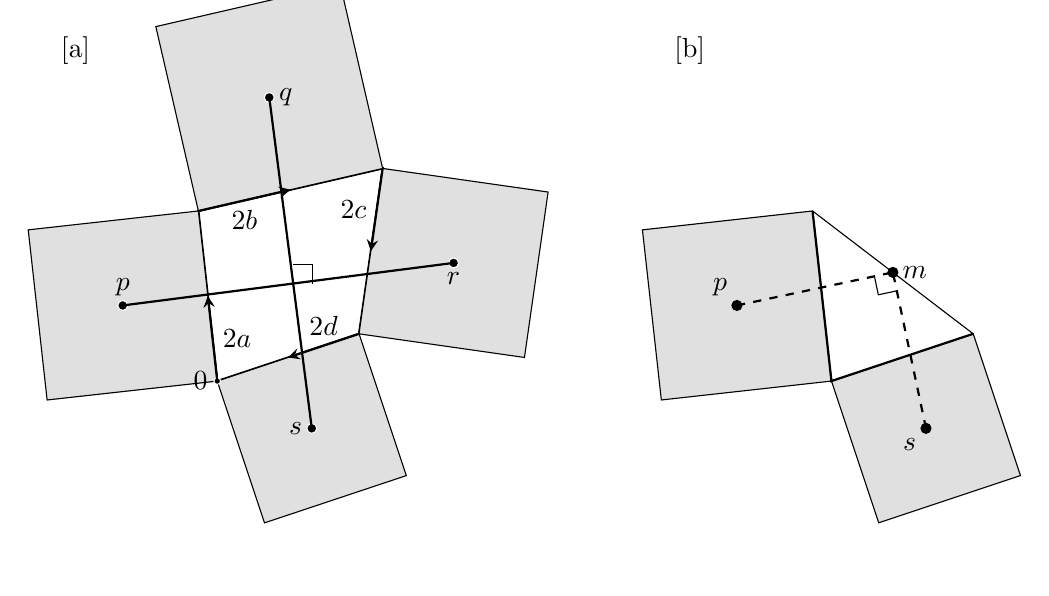
\begin{tikzpicture}[scale=1.2]
    % [a] Version
    \begin{scope}
      \node at (-1.5, 3.5) {[a]};
      % Define the quadrilateral vertices
      \coordinate (O) at (0, 0);
      \coordinate (B) at (1.5, 0.5);
      \coordinate (C) at (1.75, 2.25);
      \coordinate (D) at (-0.2, 1.8);

      % Draw the main quadrilateral (filled)
      \filldraw[fill=white!80, draw=black, thick] (O) -- (B) -- (C)
      -- (D) -- cycle;

      % Define helper for drawing squares and finding center
      % Side OA (here O to D)
      \coordinate (S1_1) at ($(O)!1!90:(D)$);
      \coordinate (S1_2) at ($(D)!1!-90:(O)$);
      \filldraw[fill=black!20!white!60, draw=black] (O) -- (D) --
      (S1_2) -- (S1_1) -- cycle;
      \coordinate (C1) at ($(O)!0.5!(S1_2)$);

      % Side AB (here D to C)
      \coordinate (S2_1) at ($(D)!1!90:(C)$);
      \coordinate (S2_2) at ($(C)!1!-90:(D)$);
      \filldraw[fill=black!20!white!60, draw=black] (D) -- (C) --
      (S2_2) -- (S2_1) -- cycle;
      \coordinate (C2) at ($(D)!0.5!(S2_2)$);

      % Side BC (here C to B)
      \coordinate (S3_1) at ($(C)!1!90:(B)$);
      \coordinate (S3_2) at ($(B)!1!-90:(C)$);
      \filldraw[fill=black!20!white!60, draw=black] (C) -- (B) --
      (S3_2) -- (S3_1) -- cycle;
      \coordinate (C3) at ($(C)!0.5!(S3_2)$);

      % Side CO (here B to O)
      \coordinate (S4_1) at ($(B)!1!90:(O)$);
      \coordinate (S4_2) at ($(O)!1!-90:(B)$);
      \filldraw[fill=black!20!white!60, draw=black] (B) -- (O) --
      (S4_2) -- (S4_1) -- cycle;
      \coordinate (C4) at ($(B)!0.5!(S4_2)$);

      % Dots for vertices and labels
      \filldraw[fill=black, draw=white] (O) circle (1pt) node[left,
      black] {$0$};
      \filldraw[fill=black, draw=white] (C1) circle (1.5pt)
      node[above, black] {$p$};
      \filldraw[fill=black, draw=white] (C2) circle (1.5pt)
      node[right, black] {$q$};
      \filldraw[fill=black, draw=white] (C3) circle (1.5pt)
      node[below, black] {$r$};
      \filldraw[fill=black, draw=white] (C4) circle (1.5pt)
      node[left, black] {$s$};

      % Lines and labels from image
      \draw[black, thick] (C1) -- (C3);
      \draw[black, thick] (C2) -- (C4);

      % Right angle marker
      \begin{scope}[shift={($(intersection of C1--C3 and C2--C4)$)}]
        \draw[black] (0, 0.2) -- (0.2, 0.2) -- (0.2, 0);
      \end{scope}

      % Vectors/labels
      \draw[->, >=stealth, black, thick] (O) -- ($(O)!0.5!(D)$)
      node[midway, right] {$2a$};
      \draw[->, >=stealth, black, thick] (D) -- ($(D)!0.5!(C)$)
      node[midway, below] {$2b$};
      \draw[->, >=stealth, black, thick] (C) -- ($(C)!0.5!(B)$)
      node[midway, left] {$2c$};
      \draw[->, >=stealth, black, thick] (B) -- ($(B)!0.5!(O)$)
      node[midway, above] {$2d$};
    \end{scope}

    % [b] Version
    \begin{scope}[xshift=6.5cm]
      \node at (-1.5, 3.5) {[b]};
      % Define the same vertices as [a]
      \coordinate (O) at (0, 0);
      \coordinate (B) at (1.5, 0.5);
      \coordinate (C) at (1.75, 2.25);
      \coordinate (D) at (-0.2, 1.8);

      % Draw the two squares involved: square on OD and square on OB
      % (or equivalent from [a])
      \filldraw[fill=black!20!white!60, draw=black] (O) -- (D) --
      ($(D)!1!-90:(O)$)-- ($(O)!1!90:(D)$) -- cycle;
      \filldraw[fill=black!20!white!60, draw=black] (B) -- (O) --
      ($(O)!1!-90:(B)$) -- ($(B)!1!90:(O)$) -- cycle;

      % Get centers p and s
      \coordinate (p) at ($(O)!0.5!($(D)!1!-90:(O)$)$);
      \coordinate (s) at ($(B)!0.5!($(O)!1!-90:(B)$)$);

      % Draw the relevant part of the quadrilateral
      \draw[black, thick] (D) -- (O) -- (B);
      \draw[black, thin] (D) -- (B);

      % Midpoint m of DB (This is the pivot in the visual proof)
      \coordinate (m) at ($(D)!0.5!(B)$);

      % Draw dashed lines connecting centers to m
      \draw[black, dashed, thick] (p) -- (m);
      \draw[black, dashed, thick] (s) -- (m);

      % Dots and labels
      \filldraw[fill=black, draw=black] (p) circle (1.5pt) node[above
      left, black] {$p$};
      \filldraw[fill=black, draw=black] (s) circle (1.5pt) node[below
      left, black] {$s$};
      \filldraw[fill=black, draw=black] (m) circle (1.5pt)
      node[right, black] {$m$};

      % Right angle marker at m
      \begin{scope}[shift={(m)}]
        \path let \p1=($(p)-(m)$), \n1={atan2(\y1,\x1)} in
        \pgfextra{\xdef\mAngle{\n1}};
        \begin{scope}[rotate=\mAngle]
          \draw[black] (0.2, 0) -- (0.2, 0.2) -- (0, 0.2);
        \end{scope}
      \end{scope}
    \end{scope}
  \end{tikzpicture}
\end{figure}

\begin{solution}
  Let the four edges of the quadrilateral be $2a, 2b, 2c, 2d$ as
  shown in the figure, and the four vertices be $O, D, C, B$ in
  counterclockwise order. For convenience, we set $O = 0$.
  Then we have:
  \[
    \begin{aligned}
      p &= a + ia \\
      q &= 2a + b + ib \\
      r &= 2a + 2b + c + ic \\
      s &= 2a + 2b + 2c + d + id \\
      0 &= a+b+c+d
    \end{aligned}
  \]
  Let $X = p - r$ and $Y = s - q$. Then we want to show that $X$ and
  $Y$ are perpendicular and of equal length, i.e., $Y = iX$.
  \[
    \begin{aligned}
      X &= p-r = -a - 2b - c + i(a - c) = -b+d+i(a-c) \\
      Y &= s-q = b + 2c + d + i (d - b) = c-a+i(d-b)
    \end{aligned}
  \]
  Thus \[
    iX = i(-b+d+i(a-c)) = c-a + i(d-b) = Y.
  \]
  So $X$ and $Y$ are perpendicular and of equal length.

\end{solution}

\subsection{Exercise 1.91}

\begin{lemma}[Lemma 1.90: Properties of the Exponential Function]
  The exponential function satisfies:
  \begin{itemize}
    \item \textbf{(EXP-1):} Its restriction to $\mathbb{R}$ is
      monotonically increasing and positive.
    \item \textbf{(EXP-2):} There exists a positive number $\pi$ such
      that $e^{\frac{\pi}{2} i} = i$ and $e^z = 1$ iff $z \in 2\pi i
      \mathbb{Z}$.
    \item \textbf{(EXP-3):} $\exp$ is periodic with period $2\pi i$.
    \item \textbf{(EXP-4):} $\theta \mapsto e^{i\theta}$ maps
      $\mathbb{R}$ onto the unit circle.
    \item \textbf{(EXP-5):} $w \in \mathbb{C} \setminus \{0\}$
      implies $w = e^z$ for some $z \in \mathbb{C}$.
  \end{itemize}
\end{lemma}

Prove Lemma 1.90 using the power series definition
$e^z = \sum_{n=0}^{\infty} \frac{z^n}{n!}$. \\
\textit{Hint: define $\cos(\theta) := \text{Re}(e^{i\theta})$,
  $\sin(\theta) := \text{Im}(e^{i\theta})$, and look for the zeros of
these functions.}

\begin{proof}
  \textbf{(EXP-1):} For real $x \in \R$, all terms in the series are
  positive for $x > 0$, so $e^x > 0$. For $x_1 < x_2$, we have
  $e^{x_1} < e^{x_2}$ since each term in $e^{x_2} - e^{x_1}$ is positive.

  \textbf{(EXP-2):} Define $\cos(\theta) = \Re(e^{i\theta})$ and
  $\sin(\theta) = \Im(e^{i\theta})$. Substituting $z = i\theta$ into the
  power series:
  \[
    e^{i\theta} = \sum_{n=0}^{\infty} \frac{(i\theta)^n}{n!}
    = \sum_{k=0}^{\infty} \frac{(-1)^k \theta^{2k}}{(2k)!}
    + i \sum_{k=0}^{\infty} \frac{(-1)^k \theta^{2k+1}}{(2k+1)!}
    = \cos\theta + i\sin\theta.
    \tag{1}
  \]
  From (1), we have $\cos^2\theta + \sin^2\theta = |e^{i\theta}|^2
  = e^{i\theta}e^{-i\theta} = 1$. Using $e^{i(\theta+\phi)} =
  e^{i\theta}e^{i\phi}$ and comparing real and imaginary parts yields
  the addition formulas for cosine and sine.

  To define $\pi$, we show that $\cos\theta$ has a unique positive zero.
  From the power series, $\cos\theta = 1 - \frac{\theta^2}{2!} +
  \frac{\theta^4}{4!} - \cdots$.
  For $0 < \theta \le 1$, we have $\cos\theta \ge 1 -
  \frac{\theta^2}{2} \ge \frac{1}{2}$.
  For $\theta = 2$, the series alternates with decreasing terms starting
  from $1 - 2^2/2! = -1$, so by the alternating series test, $\cos 2 < 0$.
  Since $\cos$ is continuous on $[1, 2]$, there exists
  $\pi_0 \in (2, 4)$ such that $\cos(\pi_0/2) = 0$. We define $\pi = \pi_0$.
  Then $\sin(\pi/2) = \sqrt{1 - \cos^2(\pi/2)} = 1$, so $e^{i\pi/2} = i$.

  Now we show $e^z = 1$ iff $z \in 2\pi i\mathbb{Z}$. First, from
  $e^{i\pi/2} = i$
  and $e^{z+w} = e^z e^w$, we have:
  \[
    e^{i\pi} = (e^{i\pi/2})^2 = i^2 = -1, \quad
    e^{i2\pi} = (e^{i\pi})^2 = (-1)^2 = 1.
  \]
  Hence $e^{2k\pi i} = 1$ for all $k \in \mathbb{Z}$.

  Conversely, suppose $e^z = 1$. Write $z = x + iy$ with $x, y \in \R$.
  Then $e^z = e^x e^{iy} = 1$ implies $e^x = 1$, so $x = 0$. Thus $e^{iy} = 1$.
  Let $y = 2k\pi + r$ with $k \in \mathbb{Z}$ and $r \in [0, 2\pi)$. Then
  $e^{iy} = e^{i2k\pi} e^{ir} = e^{ir} = 1$. So it suffices to show that
  the only solution to $e^{ir} = 1$ in $[0, 2\pi)$ is $r = 0$.

  From the power series, $e^{i\theta}$ traces a continuous path on the
  unit circle. We have shown $e^{i0} = 1$, $e^{i\pi/2} = i$, $e^{i\pi} = -1$,
  $e^{i3\pi/2} = -i$, and $e^{i2\pi} = 1$. By continuity, the equation
  $e^{ir} = 1$ can only hold at $r = 0$ within $[0, 2\pi)$. Thus $y = 2k\pi$.

  \textbf{(EXP-3):} Since $e^{2\pi i} = 1$ from (EXP-2), we have
  $e^{z + 2\pi i} = e^z e^{2\pi i} = e^z$. Conversely, if $e^{z_1} = e^{z_2}$,
  then $e^{z_1 - z_2} = 1$, so $z_1 - z_2 = 2\pi i k$ for some $k \in \Z$.

  \textbf{(EXP-4):} For any $\theta \in \R$, $|e^{i\theta}|^2 = 1$, so
  $e^{i\theta}$ lies on the unit circle. Conversely, any $w$ on the unit
  circle can be written as $w = e^{i\theta}$ for some $\theta \in \R$.

  \textbf{(EXP-5):} For $w \in \C \setminus \{0\}$, write $w = re^{i\theta}$
  with $r = |w| > 0$. Then $w = e^{\ln r + i\theta}$, where $\ln r$ is
  the real logarithm of $r$.
\end{proof}

\subsection{Exercise 1.99}
Prove $\tan(3\theta) = \frac{3T - T^3}{1 - 3T^2}$ where $T = \tan \theta$.

\begin{proof}
  First, we prove the addition formula for tangent. For any
  $\alpha, \beta \in \R$ with $\cos\alpha\cos\beta \neq 0$, we have
  \[
    \tan(\alpha + \beta)
    = \frac{\sin(\alpha + \beta)}{\cos(\alpha + \beta)}
    = \frac{\sin\alpha\cos\beta + \cos\alpha\sin\beta}
    {\cos\alpha\cos\beta - \sin\alpha\sin\beta}
    = \frac{\tan\alpha + \tan\beta}{1 - \tan\alpha\tan\beta}.
    \tag{1}
  \]

  Now compute $\tan(2\theta)$ using (1) with $\alpha = \beta = \theta$:
  \[
    \tan(2\theta) = \frac{2\tan\theta}{1 - \tan^2\theta}.
    \tag{2}
  \]

  Next, compute $\tan(3\theta) = \tan(2\theta + \theta)$ using (1) again:
  \[
    \tan(3\theta)
    = \frac{\tan(2\theta) + \tan\theta}{1 - \tan(2\theta)\tan\theta}.
  \]

  Substituting (2) into the above and letting $T = \tan\theta$:
  \[
    \begin{aligned}
      \tan(3\theta)
      &= \frac{\dfrac{2T}{1 - T^2} + T}{1 - \dfrac{2T}{1 - T^2} \cdot T} \\
      &= \frac{\dfrac{2T + T(1 - T^2)}{1 - T^2}}
      {\dfrac{1 - T^2 - 2T^2}{1 - T^2}} \\
      &= \frac{2T + T - T^3}{1 - T^2 - 2T^2} \\
      &= \frac{3T - T^3}{1 - 3T^2}.
    \end{aligned}
  \]
  This completes the proof.
\end{proof}

\subsection{Exercise 1.105}

\begin{corollary}[Corollary 1.101: Relations between Trigonometric
  and Hyperbolic Functions]
  Hyperbolic functions have period $2\pi i$ and satisfy:
  \begin{align*}
    \cosh(z+w)       & = \cosh z \cosh w + \sinh z \sinh w \\
    \sinh(z+w)       & = \sinh z \cosh w + \cosh z \sinh w \\
    \cosh z          & = \cos(iz), \quad \sinh z = -i \sin(iz) \\
    \cos z           & = \cosh(iz), \quad \sin z = -i \sinh(iz) \\
    \cosh^2 z - \sinh^2 z & = 1
  \end{align*}
\end{corollary}

What are the shapes of images of straight lines $x = \text{const}$
and $y = \text{const}$ under $z = x + iy \mapsto \cos(z)$? Draw a
dual-plane plot similar to that in Example 1.85 to answer this
question. (Hint: use Corollary 1.101)

\begin{solution}
  Using Corollary 1.101, we have
  \[
    \cos(z) = \cos(x + iy) = \cos x \cos(iy) - \sin x \sin(iy) = \cos x \cosh y - i \sin x \sinh y.
  \]
  Let $w = u + iv = \cos(z)$. Then:
  \[
    u = \cos x \cosh y, \quad v = -\sin x \sinh y.
  \]
  
  \begin{enumerate}
    \item \textbf{Vertical lines ($x = c$)}:
    If $c \neq n\pi/2$, we have $\frac{u^2}{\cos^2 c} - \frac{v^2}{\sin^2 c} = \cosh^2 y - \sinh^2 y = 1$, which represents a family of \textbf{hyperbolas}.
    \item \textbf{Horizontal lines ($y = d$)}:
    If $d > 0$, we have $\frac{u^2}{\cosh^2 d} + \frac{v^2}{\sinh^2 d} = \cos^2 x + \sin^2 x = 1$, which represents a family of \textbf{ellipses}.
  \end{enumerate}

  The dual-plane plot below (Figure \ref{fig:mapping_cos}) visualizes these conformal mappings.

  \begin{figure}[htbp]
    \centering
    \resizebox{0.9\textwidth}{!}{%% Creator: Matplotlib, PGF backend
%%
%% To include the figure in your LaTeX document, write
%%   \input{<filename>.pgf}
%%
%% Make sure the required packages are loaded in your preamble
%%   \usepackage{pgf}
%%
%% Also ensure that all the required font packages are loaded; for instance,
%% the lmodern package is sometimes necessary when using math font.
%%   \usepackage{lmodern}
%%
%% Figures using additional raster images can only be included by \input if
%% they are in the same directory as the main LaTeX file. For loading figures
%% from other directories you can use the `import` package
%%   \usepackage{import}
%%
%% and then include the figures with
%%   \import{<path to file>}{<filename>.pgf}
%%
%% Matplotlib used the following preamble
%%   \def\mathdefault#1{#1}
%%   \everymath=\expandafter{\the\everymath\displaystyle}
%%   \IfFileExists{scrextend.sty}{
%%     \usepackage[fontsize=10.000000pt]{scrextend}
%%   }{
%%     \renewcommand{\normalsize}{\fontsize{10.000000}{12.000000}\selectfont}
%%     \normalsize
%%   }
%%   \usepackage{amsmath}
%%   \usepackage{amssymb}
%%   \def\mathdefault#1{#1}
%%   \makeatletter\@ifpackageloaded{underscore}{}{\usepackage[strings]{underscore}}\makeatother
%%
\begingroup%
\makeatletter%
\begin{pgfpicture}%
\pgfpathrectangle{\pgfpointorigin}{\pgfqpoint{10.000000in}{4.500000in}}%
\pgfusepath{use as bounding box, clip}%
\begin{pgfscope}%
\pgfsetbuttcap%
\pgfsetmiterjoin%
\definecolor{currentfill}{rgb}{1.000000,1.000000,1.000000}%
\pgfsetfillcolor{currentfill}%
\pgfsetlinewidth{0.000000pt}%
\definecolor{currentstroke}{rgb}{1.000000,1.000000,1.000000}%
\pgfsetstrokecolor{currentstroke}%
\pgfsetdash{}{0pt}%
\pgfpathmoveto{\pgfqpoint{0.000000in}{0.000000in}}%
\pgfpathlineto{\pgfqpoint{10.000000in}{0.000000in}}%
\pgfpathlineto{\pgfqpoint{10.000000in}{4.500000in}}%
\pgfpathlineto{\pgfqpoint{0.000000in}{4.500000in}}%
\pgfpathlineto{\pgfqpoint{0.000000in}{0.000000in}}%
\pgfpathclose%
\pgfusepath{fill}%
\end{pgfscope}%
\begin{pgfscope}%
\pgfsetbuttcap%
\pgfsetmiterjoin%
\definecolor{currentfill}{rgb}{1.000000,1.000000,1.000000}%
\pgfsetfillcolor{currentfill}%
\pgfsetlinewidth{0.000000pt}%
\definecolor{currentstroke}{rgb}{0.000000,0.000000,0.000000}%
\pgfsetstrokecolor{currentstroke}%
\pgfsetstrokeopacity{0.000000}%
\pgfsetdash{}{0pt}%
\pgfpathmoveto{\pgfqpoint{0.495251in}{1.287254in}}%
\pgfpathlineto{\pgfqpoint{4.932639in}{1.287254in}}%
\pgfpathlineto{\pgfqpoint{4.932639in}{3.212746in}}%
\pgfpathlineto{\pgfqpoint{0.495251in}{3.212746in}}%
\pgfpathlineto{\pgfqpoint{0.495251in}{1.287254in}}%
\pgfpathclose%
\pgfusepath{fill}%
\end{pgfscope}%
\begin{pgfscope}%
\pgfpathrectangle{\pgfqpoint{0.495251in}{1.287254in}}{\pgfqpoint{4.437388in}{1.925493in}}%
\pgfusepath{clip}%
\pgfsetrectcap%
\pgfsetroundjoin%
\pgfsetlinewidth{0.803000pt}%
\definecolor{currentstroke}{rgb}{0.690196,0.690196,0.690196}%
\pgfsetstrokecolor{currentstroke}%
\pgfsetstrokeopacity{0.300000}%
\pgfsetdash{}{0pt}%
\pgfpathmoveto{\pgfqpoint{0.628043in}{1.287254in}}%
\pgfpathlineto{\pgfqpoint{0.628043in}{3.212746in}}%
\pgfusepath{stroke}%
\end{pgfscope}%
\begin{pgfscope}%
\pgfsetbuttcap%
\pgfsetroundjoin%
\definecolor{currentfill}{rgb}{0.000000,0.000000,0.000000}%
\pgfsetfillcolor{currentfill}%
\pgfsetlinewidth{0.803000pt}%
\definecolor{currentstroke}{rgb}{0.000000,0.000000,0.000000}%
\pgfsetstrokecolor{currentstroke}%
\pgfsetdash{}{0pt}%
\pgfsys@defobject{currentmarker}{\pgfqpoint{0.000000in}{-0.048611in}}{\pgfqpoint{0.000000in}{0.000000in}}{%
\pgfpathmoveto{\pgfqpoint{0.000000in}{0.000000in}}%
\pgfpathlineto{\pgfqpoint{0.000000in}{-0.048611in}}%
\pgfusepath{stroke,fill}%
}%
\begin{pgfscope}%
\pgfsys@transformshift{0.628043in}{1.287254in}%
\pgfsys@useobject{currentmarker}{}%
\end{pgfscope}%
\end{pgfscope}%
\begin{pgfscope}%
\definecolor{textcolor}{rgb}{0.000000,0.000000,0.000000}%
\pgfsetstrokecolor{textcolor}%
\pgfsetfillcolor{textcolor}%
\pgftext[x=0.628043in,y=1.190031in,,top]{\color{textcolor}{\rmfamily\fontsize{10.000000}{12.000000}\selectfont\catcode`\^=\active\def^{\ifmmode\sp\else\^{}\fi}\catcode`\%=\active\def%{\%}$-\pi$}}%
\end{pgfscope}%
\begin{pgfscope}%
\pgfpathrectangle{\pgfqpoint{0.495251in}{1.287254in}}{\pgfqpoint{4.437388in}{1.925493in}}%
\pgfusepath{clip}%
\pgfsetrectcap%
\pgfsetroundjoin%
\pgfsetlinewidth{0.803000pt}%
\definecolor{currentstroke}{rgb}{0.690196,0.690196,0.690196}%
\pgfsetstrokecolor{currentstroke}%
\pgfsetstrokeopacity{0.300000}%
\pgfsetdash{}{0pt}%
\pgfpathmoveto{\pgfqpoint{1.670994in}{1.287254in}}%
\pgfpathlineto{\pgfqpoint{1.670994in}{3.212746in}}%
\pgfusepath{stroke}%
\end{pgfscope}%
\begin{pgfscope}%
\pgfsetbuttcap%
\pgfsetroundjoin%
\definecolor{currentfill}{rgb}{0.000000,0.000000,0.000000}%
\pgfsetfillcolor{currentfill}%
\pgfsetlinewidth{0.803000pt}%
\definecolor{currentstroke}{rgb}{0.000000,0.000000,0.000000}%
\pgfsetstrokecolor{currentstroke}%
\pgfsetdash{}{0pt}%
\pgfsys@defobject{currentmarker}{\pgfqpoint{0.000000in}{-0.048611in}}{\pgfqpoint{0.000000in}{0.000000in}}{%
\pgfpathmoveto{\pgfqpoint{0.000000in}{0.000000in}}%
\pgfpathlineto{\pgfqpoint{0.000000in}{-0.048611in}}%
\pgfusepath{stroke,fill}%
}%
\begin{pgfscope}%
\pgfsys@transformshift{1.670994in}{1.287254in}%
\pgfsys@useobject{currentmarker}{}%
\end{pgfscope}%
\end{pgfscope}%
\begin{pgfscope}%
\definecolor{textcolor}{rgb}{0.000000,0.000000,0.000000}%
\pgfsetstrokecolor{textcolor}%
\pgfsetfillcolor{textcolor}%
\pgftext[x=1.670994in,y=1.190031in,,top]{\color{textcolor}{\rmfamily\fontsize{10.000000}{12.000000}\selectfont\catcode`\^=\active\def^{\ifmmode\sp\else\^{}\fi}\catcode`\%=\active\def%{\%}$-\pi/2$}}%
\end{pgfscope}%
\begin{pgfscope}%
\pgfpathrectangle{\pgfqpoint{0.495251in}{1.287254in}}{\pgfqpoint{4.437388in}{1.925493in}}%
\pgfusepath{clip}%
\pgfsetrectcap%
\pgfsetroundjoin%
\pgfsetlinewidth{0.803000pt}%
\definecolor{currentstroke}{rgb}{0.690196,0.690196,0.690196}%
\pgfsetstrokecolor{currentstroke}%
\pgfsetstrokeopacity{0.300000}%
\pgfsetdash{}{0pt}%
\pgfpathmoveto{\pgfqpoint{2.713945in}{1.287254in}}%
\pgfpathlineto{\pgfqpoint{2.713945in}{3.212746in}}%
\pgfusepath{stroke}%
\end{pgfscope}%
\begin{pgfscope}%
\pgfsetbuttcap%
\pgfsetroundjoin%
\definecolor{currentfill}{rgb}{0.000000,0.000000,0.000000}%
\pgfsetfillcolor{currentfill}%
\pgfsetlinewidth{0.803000pt}%
\definecolor{currentstroke}{rgb}{0.000000,0.000000,0.000000}%
\pgfsetstrokecolor{currentstroke}%
\pgfsetdash{}{0pt}%
\pgfsys@defobject{currentmarker}{\pgfqpoint{0.000000in}{-0.048611in}}{\pgfqpoint{0.000000in}{0.000000in}}{%
\pgfpathmoveto{\pgfqpoint{0.000000in}{0.000000in}}%
\pgfpathlineto{\pgfqpoint{0.000000in}{-0.048611in}}%
\pgfusepath{stroke,fill}%
}%
\begin{pgfscope}%
\pgfsys@transformshift{2.713945in}{1.287254in}%
\pgfsys@useobject{currentmarker}{}%
\end{pgfscope}%
\end{pgfscope}%
\begin{pgfscope}%
\definecolor{textcolor}{rgb}{0.000000,0.000000,0.000000}%
\pgfsetstrokecolor{textcolor}%
\pgfsetfillcolor{textcolor}%
\pgftext[x=2.713945in,y=1.190031in,,top]{\color{textcolor}{\rmfamily\fontsize{10.000000}{12.000000}\selectfont\catcode`\^=\active\def^{\ifmmode\sp\else\^{}\fi}\catcode`\%=\active\def%{\%}$0$}}%
\end{pgfscope}%
\begin{pgfscope}%
\pgfpathrectangle{\pgfqpoint{0.495251in}{1.287254in}}{\pgfqpoint{4.437388in}{1.925493in}}%
\pgfusepath{clip}%
\pgfsetrectcap%
\pgfsetroundjoin%
\pgfsetlinewidth{0.803000pt}%
\definecolor{currentstroke}{rgb}{0.690196,0.690196,0.690196}%
\pgfsetstrokecolor{currentstroke}%
\pgfsetstrokeopacity{0.300000}%
\pgfsetdash{}{0pt}%
\pgfpathmoveto{\pgfqpoint{3.756896in}{1.287254in}}%
\pgfpathlineto{\pgfqpoint{3.756896in}{3.212746in}}%
\pgfusepath{stroke}%
\end{pgfscope}%
\begin{pgfscope}%
\pgfsetbuttcap%
\pgfsetroundjoin%
\definecolor{currentfill}{rgb}{0.000000,0.000000,0.000000}%
\pgfsetfillcolor{currentfill}%
\pgfsetlinewidth{0.803000pt}%
\definecolor{currentstroke}{rgb}{0.000000,0.000000,0.000000}%
\pgfsetstrokecolor{currentstroke}%
\pgfsetdash{}{0pt}%
\pgfsys@defobject{currentmarker}{\pgfqpoint{0.000000in}{-0.048611in}}{\pgfqpoint{0.000000in}{0.000000in}}{%
\pgfpathmoveto{\pgfqpoint{0.000000in}{0.000000in}}%
\pgfpathlineto{\pgfqpoint{0.000000in}{-0.048611in}}%
\pgfusepath{stroke,fill}%
}%
\begin{pgfscope}%
\pgfsys@transformshift{3.756896in}{1.287254in}%
\pgfsys@useobject{currentmarker}{}%
\end{pgfscope}%
\end{pgfscope}%
\begin{pgfscope}%
\definecolor{textcolor}{rgb}{0.000000,0.000000,0.000000}%
\pgfsetstrokecolor{textcolor}%
\pgfsetfillcolor{textcolor}%
\pgftext[x=3.756896in,y=1.190031in,,top]{\color{textcolor}{\rmfamily\fontsize{10.000000}{12.000000}\selectfont\catcode`\^=\active\def^{\ifmmode\sp\else\^{}\fi}\catcode`\%=\active\def%{\%}$\pi/2$}}%
\end{pgfscope}%
\begin{pgfscope}%
\pgfpathrectangle{\pgfqpoint{0.495251in}{1.287254in}}{\pgfqpoint{4.437388in}{1.925493in}}%
\pgfusepath{clip}%
\pgfsetrectcap%
\pgfsetroundjoin%
\pgfsetlinewidth{0.803000pt}%
\definecolor{currentstroke}{rgb}{0.690196,0.690196,0.690196}%
\pgfsetstrokecolor{currentstroke}%
\pgfsetstrokeopacity{0.300000}%
\pgfsetdash{}{0pt}%
\pgfpathmoveto{\pgfqpoint{4.799846in}{1.287254in}}%
\pgfpathlineto{\pgfqpoint{4.799846in}{3.212746in}}%
\pgfusepath{stroke}%
\end{pgfscope}%
\begin{pgfscope}%
\pgfsetbuttcap%
\pgfsetroundjoin%
\definecolor{currentfill}{rgb}{0.000000,0.000000,0.000000}%
\pgfsetfillcolor{currentfill}%
\pgfsetlinewidth{0.803000pt}%
\definecolor{currentstroke}{rgb}{0.000000,0.000000,0.000000}%
\pgfsetstrokecolor{currentstroke}%
\pgfsetdash{}{0pt}%
\pgfsys@defobject{currentmarker}{\pgfqpoint{0.000000in}{-0.048611in}}{\pgfqpoint{0.000000in}{0.000000in}}{%
\pgfpathmoveto{\pgfqpoint{0.000000in}{0.000000in}}%
\pgfpathlineto{\pgfqpoint{0.000000in}{-0.048611in}}%
\pgfusepath{stroke,fill}%
}%
\begin{pgfscope}%
\pgfsys@transformshift{4.799846in}{1.287254in}%
\pgfsys@useobject{currentmarker}{}%
\end{pgfscope}%
\end{pgfscope}%
\begin{pgfscope}%
\definecolor{textcolor}{rgb}{0.000000,0.000000,0.000000}%
\pgfsetstrokecolor{textcolor}%
\pgfsetfillcolor{textcolor}%
\pgftext[x=4.799846in,y=1.190031in,,top]{\color{textcolor}{\rmfamily\fontsize{10.000000}{12.000000}\selectfont\catcode`\^=\active\def^{\ifmmode\sp\else\^{}\fi}\catcode`\%=\active\def%{\%}$\pi$}}%
\end{pgfscope}%
\begin{pgfscope}%
\definecolor{textcolor}{rgb}{0.000000,0.000000,0.000000}%
\pgfsetstrokecolor{textcolor}%
\pgfsetfillcolor{textcolor}%
\pgftext[x=2.713945in,y=0.995587in,,top]{\color{textcolor}{\rmfamily\fontsize{10.000000}{12.000000}\selectfont\catcode`\^=\active\def^{\ifmmode\sp\else\^{}\fi}\catcode`\%=\active\def%{\%}$x$}}%
\end{pgfscope}%
\begin{pgfscope}%
\pgfpathrectangle{\pgfqpoint{0.495251in}{1.287254in}}{\pgfqpoint{4.437388in}{1.925493in}}%
\pgfusepath{clip}%
\pgfsetrectcap%
\pgfsetroundjoin%
\pgfsetlinewidth{0.803000pt}%
\definecolor{currentstroke}{rgb}{0.690196,0.690196,0.690196}%
\pgfsetstrokecolor{currentstroke}%
\pgfsetstrokeopacity{0.300000}%
\pgfsetdash{}{0pt}%
\pgfpathmoveto{\pgfqpoint{0.495251in}{1.420046in}}%
\pgfpathlineto{\pgfqpoint{4.932639in}{1.420046in}}%
\pgfusepath{stroke}%
\end{pgfscope}%
\begin{pgfscope}%
\pgfsetbuttcap%
\pgfsetroundjoin%
\definecolor{currentfill}{rgb}{0.000000,0.000000,0.000000}%
\pgfsetfillcolor{currentfill}%
\pgfsetlinewidth{0.803000pt}%
\definecolor{currentstroke}{rgb}{0.000000,0.000000,0.000000}%
\pgfsetstrokecolor{currentstroke}%
\pgfsetdash{}{0pt}%
\pgfsys@defobject{currentmarker}{\pgfqpoint{-0.048611in}{0.000000in}}{\pgfqpoint{-0.000000in}{0.000000in}}{%
\pgfpathmoveto{\pgfqpoint{-0.000000in}{0.000000in}}%
\pgfpathlineto{\pgfqpoint{-0.048611in}{0.000000in}}%
\pgfusepath{stroke,fill}%
}%
\begin{pgfscope}%
\pgfsys@transformshift{0.495251in}{1.420046in}%
\pgfsys@useobject{currentmarker}{}%
\end{pgfscope}%
\end{pgfscope}%
\begin{pgfscope}%
\definecolor{textcolor}{rgb}{0.000000,0.000000,0.000000}%
\pgfsetstrokecolor{textcolor}%
\pgfsetfillcolor{textcolor}%
\pgftext[x=0.220559in, y=1.371852in, left, base]{\color{textcolor}{\rmfamily\fontsize{10.000000}{12.000000}\selectfont\catcode`\^=\active\def^{\ifmmode\sp\else\^{}\fi}\catcode`\%=\active\def%{\%}$\mathdefault{0.0}$}}%
\end{pgfscope}%
\begin{pgfscope}%
\pgfpathrectangle{\pgfqpoint{0.495251in}{1.287254in}}{\pgfqpoint{4.437388in}{1.925493in}}%
\pgfusepath{clip}%
\pgfsetrectcap%
\pgfsetroundjoin%
\pgfsetlinewidth{0.803000pt}%
\definecolor{currentstroke}{rgb}{0.690196,0.690196,0.690196}%
\pgfsetstrokecolor{currentstroke}%
\pgfsetstrokeopacity{0.300000}%
\pgfsetdash{}{0pt}%
\pgfpathmoveto{\pgfqpoint{0.495251in}{1.752028in}}%
\pgfpathlineto{\pgfqpoint{4.932639in}{1.752028in}}%
\pgfusepath{stroke}%
\end{pgfscope}%
\begin{pgfscope}%
\pgfsetbuttcap%
\pgfsetroundjoin%
\definecolor{currentfill}{rgb}{0.000000,0.000000,0.000000}%
\pgfsetfillcolor{currentfill}%
\pgfsetlinewidth{0.803000pt}%
\definecolor{currentstroke}{rgb}{0.000000,0.000000,0.000000}%
\pgfsetstrokecolor{currentstroke}%
\pgfsetdash{}{0pt}%
\pgfsys@defobject{currentmarker}{\pgfqpoint{-0.048611in}{0.000000in}}{\pgfqpoint{-0.000000in}{0.000000in}}{%
\pgfpathmoveto{\pgfqpoint{-0.000000in}{0.000000in}}%
\pgfpathlineto{\pgfqpoint{-0.048611in}{0.000000in}}%
\pgfusepath{stroke,fill}%
}%
\begin{pgfscope}%
\pgfsys@transformshift{0.495251in}{1.752028in}%
\pgfsys@useobject{currentmarker}{}%
\end{pgfscope}%
\end{pgfscope}%
\begin{pgfscope}%
\definecolor{textcolor}{rgb}{0.000000,0.000000,0.000000}%
\pgfsetstrokecolor{textcolor}%
\pgfsetfillcolor{textcolor}%
\pgftext[x=0.220559in, y=1.703833in, left, base]{\color{textcolor}{\rmfamily\fontsize{10.000000}{12.000000}\selectfont\catcode`\^=\active\def^{\ifmmode\sp\else\^{}\fi}\catcode`\%=\active\def%{\%}$\mathdefault{0.5}$}}%
\end{pgfscope}%
\begin{pgfscope}%
\pgfpathrectangle{\pgfqpoint{0.495251in}{1.287254in}}{\pgfqpoint{4.437388in}{1.925493in}}%
\pgfusepath{clip}%
\pgfsetrectcap%
\pgfsetroundjoin%
\pgfsetlinewidth{0.803000pt}%
\definecolor{currentstroke}{rgb}{0.690196,0.690196,0.690196}%
\pgfsetstrokecolor{currentstroke}%
\pgfsetstrokeopacity{0.300000}%
\pgfsetdash{}{0pt}%
\pgfpathmoveto{\pgfqpoint{0.495251in}{2.084009in}}%
\pgfpathlineto{\pgfqpoint{4.932639in}{2.084009in}}%
\pgfusepath{stroke}%
\end{pgfscope}%
\begin{pgfscope}%
\pgfsetbuttcap%
\pgfsetroundjoin%
\definecolor{currentfill}{rgb}{0.000000,0.000000,0.000000}%
\pgfsetfillcolor{currentfill}%
\pgfsetlinewidth{0.803000pt}%
\definecolor{currentstroke}{rgb}{0.000000,0.000000,0.000000}%
\pgfsetstrokecolor{currentstroke}%
\pgfsetdash{}{0pt}%
\pgfsys@defobject{currentmarker}{\pgfqpoint{-0.048611in}{0.000000in}}{\pgfqpoint{-0.000000in}{0.000000in}}{%
\pgfpathmoveto{\pgfqpoint{-0.000000in}{0.000000in}}%
\pgfpathlineto{\pgfqpoint{-0.048611in}{0.000000in}}%
\pgfusepath{stroke,fill}%
}%
\begin{pgfscope}%
\pgfsys@transformshift{0.495251in}{2.084009in}%
\pgfsys@useobject{currentmarker}{}%
\end{pgfscope}%
\end{pgfscope}%
\begin{pgfscope}%
\definecolor{textcolor}{rgb}{0.000000,0.000000,0.000000}%
\pgfsetstrokecolor{textcolor}%
\pgfsetfillcolor{textcolor}%
\pgftext[x=0.220559in, y=2.035815in, left, base]{\color{textcolor}{\rmfamily\fontsize{10.000000}{12.000000}\selectfont\catcode`\^=\active\def^{\ifmmode\sp\else\^{}\fi}\catcode`\%=\active\def%{\%}$\mathdefault{1.0}$}}%
\end{pgfscope}%
\begin{pgfscope}%
\pgfpathrectangle{\pgfqpoint{0.495251in}{1.287254in}}{\pgfqpoint{4.437388in}{1.925493in}}%
\pgfusepath{clip}%
\pgfsetrectcap%
\pgfsetroundjoin%
\pgfsetlinewidth{0.803000pt}%
\definecolor{currentstroke}{rgb}{0.690196,0.690196,0.690196}%
\pgfsetstrokecolor{currentstroke}%
\pgfsetstrokeopacity{0.300000}%
\pgfsetdash{}{0pt}%
\pgfpathmoveto{\pgfqpoint{0.495251in}{2.415991in}}%
\pgfpathlineto{\pgfqpoint{4.932639in}{2.415991in}}%
\pgfusepath{stroke}%
\end{pgfscope}%
\begin{pgfscope}%
\pgfsetbuttcap%
\pgfsetroundjoin%
\definecolor{currentfill}{rgb}{0.000000,0.000000,0.000000}%
\pgfsetfillcolor{currentfill}%
\pgfsetlinewidth{0.803000pt}%
\definecolor{currentstroke}{rgb}{0.000000,0.000000,0.000000}%
\pgfsetstrokecolor{currentstroke}%
\pgfsetdash{}{0pt}%
\pgfsys@defobject{currentmarker}{\pgfqpoint{-0.048611in}{0.000000in}}{\pgfqpoint{-0.000000in}{0.000000in}}{%
\pgfpathmoveto{\pgfqpoint{-0.000000in}{0.000000in}}%
\pgfpathlineto{\pgfqpoint{-0.048611in}{0.000000in}}%
\pgfusepath{stroke,fill}%
}%
\begin{pgfscope}%
\pgfsys@transformshift{0.495251in}{2.415991in}%
\pgfsys@useobject{currentmarker}{}%
\end{pgfscope}%
\end{pgfscope}%
\begin{pgfscope}%
\definecolor{textcolor}{rgb}{0.000000,0.000000,0.000000}%
\pgfsetstrokecolor{textcolor}%
\pgfsetfillcolor{textcolor}%
\pgftext[x=0.220559in, y=2.367796in, left, base]{\color{textcolor}{\rmfamily\fontsize{10.000000}{12.000000}\selectfont\catcode`\^=\active\def^{\ifmmode\sp\else\^{}\fi}\catcode`\%=\active\def%{\%}$\mathdefault{1.5}$}}%
\end{pgfscope}%
\begin{pgfscope}%
\pgfpathrectangle{\pgfqpoint{0.495251in}{1.287254in}}{\pgfqpoint{4.437388in}{1.925493in}}%
\pgfusepath{clip}%
\pgfsetrectcap%
\pgfsetroundjoin%
\pgfsetlinewidth{0.803000pt}%
\definecolor{currentstroke}{rgb}{0.690196,0.690196,0.690196}%
\pgfsetstrokecolor{currentstroke}%
\pgfsetstrokeopacity{0.300000}%
\pgfsetdash{}{0pt}%
\pgfpathmoveto{\pgfqpoint{0.495251in}{2.747972in}}%
\pgfpathlineto{\pgfqpoint{4.932639in}{2.747972in}}%
\pgfusepath{stroke}%
\end{pgfscope}%
\begin{pgfscope}%
\pgfsetbuttcap%
\pgfsetroundjoin%
\definecolor{currentfill}{rgb}{0.000000,0.000000,0.000000}%
\pgfsetfillcolor{currentfill}%
\pgfsetlinewidth{0.803000pt}%
\definecolor{currentstroke}{rgb}{0.000000,0.000000,0.000000}%
\pgfsetstrokecolor{currentstroke}%
\pgfsetdash{}{0pt}%
\pgfsys@defobject{currentmarker}{\pgfqpoint{-0.048611in}{0.000000in}}{\pgfqpoint{-0.000000in}{0.000000in}}{%
\pgfpathmoveto{\pgfqpoint{-0.000000in}{0.000000in}}%
\pgfpathlineto{\pgfqpoint{-0.048611in}{0.000000in}}%
\pgfusepath{stroke,fill}%
}%
\begin{pgfscope}%
\pgfsys@transformshift{0.495251in}{2.747972in}%
\pgfsys@useobject{currentmarker}{}%
\end{pgfscope}%
\end{pgfscope}%
\begin{pgfscope}%
\definecolor{textcolor}{rgb}{0.000000,0.000000,0.000000}%
\pgfsetstrokecolor{textcolor}%
\pgfsetfillcolor{textcolor}%
\pgftext[x=0.220559in, y=2.699778in, left, base]{\color{textcolor}{\rmfamily\fontsize{10.000000}{12.000000}\selectfont\catcode`\^=\active\def^{\ifmmode\sp\else\^{}\fi}\catcode`\%=\active\def%{\%}$\mathdefault{2.0}$}}%
\end{pgfscope}%
\begin{pgfscope}%
\pgfpathrectangle{\pgfqpoint{0.495251in}{1.287254in}}{\pgfqpoint{4.437388in}{1.925493in}}%
\pgfusepath{clip}%
\pgfsetrectcap%
\pgfsetroundjoin%
\pgfsetlinewidth{0.803000pt}%
\definecolor{currentstroke}{rgb}{0.690196,0.690196,0.690196}%
\pgfsetstrokecolor{currentstroke}%
\pgfsetstrokeopacity{0.300000}%
\pgfsetdash{}{0pt}%
\pgfpathmoveto{\pgfqpoint{0.495251in}{3.079954in}}%
\pgfpathlineto{\pgfqpoint{4.932639in}{3.079954in}}%
\pgfusepath{stroke}%
\end{pgfscope}%
\begin{pgfscope}%
\pgfsetbuttcap%
\pgfsetroundjoin%
\definecolor{currentfill}{rgb}{0.000000,0.000000,0.000000}%
\pgfsetfillcolor{currentfill}%
\pgfsetlinewidth{0.803000pt}%
\definecolor{currentstroke}{rgb}{0.000000,0.000000,0.000000}%
\pgfsetstrokecolor{currentstroke}%
\pgfsetdash{}{0pt}%
\pgfsys@defobject{currentmarker}{\pgfqpoint{-0.048611in}{0.000000in}}{\pgfqpoint{-0.000000in}{0.000000in}}{%
\pgfpathmoveto{\pgfqpoint{-0.000000in}{0.000000in}}%
\pgfpathlineto{\pgfqpoint{-0.048611in}{0.000000in}}%
\pgfusepath{stroke,fill}%
}%
\begin{pgfscope}%
\pgfsys@transformshift{0.495251in}{3.079954in}%
\pgfsys@useobject{currentmarker}{}%
\end{pgfscope}%
\end{pgfscope}%
\begin{pgfscope}%
\definecolor{textcolor}{rgb}{0.000000,0.000000,0.000000}%
\pgfsetstrokecolor{textcolor}%
\pgfsetfillcolor{textcolor}%
\pgftext[x=0.220559in, y=3.031759in, left, base]{\color{textcolor}{\rmfamily\fontsize{10.000000}{12.000000}\selectfont\catcode`\^=\active\def^{\ifmmode\sp\else\^{}\fi}\catcode`\%=\active\def%{\%}$\mathdefault{2.5}$}}%
\end{pgfscope}%
\begin{pgfscope}%
\definecolor{textcolor}{rgb}{0.000000,0.000000,0.000000}%
\pgfsetstrokecolor{textcolor}%
\pgfsetfillcolor{textcolor}%
\pgftext[x=0.165003in,y=2.250000in,,bottom,rotate=90.000000]{\color{textcolor}{\rmfamily\fontsize{10.000000}{12.000000}\selectfont\catcode`\^=\active\def^{\ifmmode\sp\else\^{}\fi}\catcode`\%=\active\def%{\%}$y$}}%
\end{pgfscope}%
\begin{pgfscope}%
\pgfpathrectangle{\pgfqpoint{0.495251in}{1.287254in}}{\pgfqpoint{4.437388in}{1.925493in}}%
\pgfusepath{clip}%
\pgfsetrectcap%
\pgfsetroundjoin%
\pgfsetlinewidth{1.505625pt}%
\definecolor{currentstroke}{rgb}{0.267004,0.004874,0.329415}%
\pgfsetstrokecolor{currentstroke}%
\pgfsetstrokeopacity{0.800000}%
\pgfsetdash{}{0pt}%
\pgfpathmoveto{\pgfqpoint{0.628043in}{1.420046in}}%
\pgfpathlineto{\pgfqpoint{0.628043in}{3.079954in}}%
\pgfpathlineto{\pgfqpoint{0.628043in}{3.079954in}}%
\pgfusepath{stroke}%
\end{pgfscope}%
\begin{pgfscope}%
\pgfpathrectangle{\pgfqpoint{0.495251in}{1.287254in}}{\pgfqpoint{4.437388in}{1.925493in}}%
\pgfusepath{clip}%
\pgfsetrectcap%
\pgfsetroundjoin%
\pgfsetlinewidth{1.505625pt}%
\definecolor{currentstroke}{rgb}{0.283229,0.120777,0.440584}%
\pgfsetstrokecolor{currentstroke}%
\pgfsetstrokeopacity{0.800000}%
\pgfsetdash{}{0pt}%
\pgfpathmoveto{\pgfqpoint{0.975694in}{1.420046in}}%
\pgfpathlineto{\pgfqpoint{0.975694in}{3.079954in}}%
\pgfpathlineto{\pgfqpoint{0.975694in}{3.079954in}}%
\pgfusepath{stroke}%
\end{pgfscope}%
\begin{pgfscope}%
\pgfpathrectangle{\pgfqpoint{0.495251in}{1.287254in}}{\pgfqpoint{4.437388in}{1.925493in}}%
\pgfusepath{clip}%
\pgfsetrectcap%
\pgfsetroundjoin%
\pgfsetlinewidth{1.505625pt}%
\definecolor{currentstroke}{rgb}{0.267968,0.223549,0.512008}%
\pgfsetstrokecolor{currentstroke}%
\pgfsetstrokeopacity{0.800000}%
\pgfsetdash{}{0pt}%
\pgfpathmoveto{\pgfqpoint{1.323344in}{1.420046in}}%
\pgfpathlineto{\pgfqpoint{1.323344in}{3.079954in}}%
\pgfpathlineto{\pgfqpoint{1.323344in}{3.079954in}}%
\pgfusepath{stroke}%
\end{pgfscope}%
\begin{pgfscope}%
\pgfpathrectangle{\pgfqpoint{0.495251in}{1.287254in}}{\pgfqpoint{4.437388in}{1.925493in}}%
\pgfusepath{clip}%
\pgfsetrectcap%
\pgfsetroundjoin%
\pgfsetlinewidth{1.505625pt}%
\definecolor{currentstroke}{rgb}{0.229739,0.322361,0.545706}%
\pgfsetstrokecolor{currentstroke}%
\pgfsetstrokeopacity{0.800000}%
\pgfsetdash{}{0pt}%
\pgfpathmoveto{\pgfqpoint{1.670994in}{1.420046in}}%
\pgfpathlineto{\pgfqpoint{1.670994in}{3.079954in}}%
\pgfpathlineto{\pgfqpoint{1.670994in}{3.079954in}}%
\pgfusepath{stroke}%
\end{pgfscope}%
\begin{pgfscope}%
\pgfpathrectangle{\pgfqpoint{0.495251in}{1.287254in}}{\pgfqpoint{4.437388in}{1.925493in}}%
\pgfusepath{clip}%
\pgfsetrectcap%
\pgfsetroundjoin%
\pgfsetlinewidth{1.505625pt}%
\definecolor{currentstroke}{rgb}{0.190631,0.407061,0.556089}%
\pgfsetstrokecolor{currentstroke}%
\pgfsetstrokeopacity{0.800000}%
\pgfsetdash{}{0pt}%
\pgfpathmoveto{\pgfqpoint{2.018644in}{1.420046in}}%
\pgfpathlineto{\pgfqpoint{2.018644in}{3.079954in}}%
\pgfpathlineto{\pgfqpoint{2.018644in}{3.079954in}}%
\pgfusepath{stroke}%
\end{pgfscope}%
\begin{pgfscope}%
\pgfpathrectangle{\pgfqpoint{0.495251in}{1.287254in}}{\pgfqpoint{4.437388in}{1.925493in}}%
\pgfusepath{clip}%
\pgfsetrectcap%
\pgfsetroundjoin%
\pgfsetlinewidth{1.505625pt}%
\definecolor{currentstroke}{rgb}{0.157729,0.485932,0.558013}%
\pgfsetstrokecolor{currentstroke}%
\pgfsetstrokeopacity{0.800000}%
\pgfsetdash{}{0pt}%
\pgfpathmoveto{\pgfqpoint{2.366295in}{1.420046in}}%
\pgfpathlineto{\pgfqpoint{2.366295in}{3.079954in}}%
\pgfpathlineto{\pgfqpoint{2.366295in}{3.079954in}}%
\pgfusepath{stroke}%
\end{pgfscope}%
\begin{pgfscope}%
\pgfpathrectangle{\pgfqpoint{0.495251in}{1.287254in}}{\pgfqpoint{4.437388in}{1.925493in}}%
\pgfusepath{clip}%
\pgfsetrectcap%
\pgfsetroundjoin%
\pgfsetlinewidth{1.505625pt}%
\definecolor{currentstroke}{rgb}{0.127568,0.566949,0.550556}%
\pgfsetstrokecolor{currentstroke}%
\pgfsetstrokeopacity{0.800000}%
\pgfsetdash{}{0pt}%
\pgfpathmoveto{\pgfqpoint{2.713945in}{1.420046in}}%
\pgfpathlineto{\pgfqpoint{2.713945in}{3.079954in}}%
\pgfpathlineto{\pgfqpoint{2.713945in}{3.079954in}}%
\pgfusepath{stroke}%
\end{pgfscope}%
\begin{pgfscope}%
\pgfpathrectangle{\pgfqpoint{0.495251in}{1.287254in}}{\pgfqpoint{4.437388in}{1.925493in}}%
\pgfusepath{clip}%
\pgfsetrectcap%
\pgfsetroundjoin%
\pgfsetlinewidth{1.505625pt}%
\definecolor{currentstroke}{rgb}{0.126326,0.644107,0.525311}%
\pgfsetstrokecolor{currentstroke}%
\pgfsetstrokeopacity{0.800000}%
\pgfsetdash{}{0pt}%
\pgfpathmoveto{\pgfqpoint{3.061595in}{1.420046in}}%
\pgfpathlineto{\pgfqpoint{3.061595in}{3.079954in}}%
\pgfpathlineto{\pgfqpoint{3.061595in}{3.079954in}}%
\pgfusepath{stroke}%
\end{pgfscope}%
\begin{pgfscope}%
\pgfpathrectangle{\pgfqpoint{0.495251in}{1.287254in}}{\pgfqpoint{4.437388in}{1.925493in}}%
\pgfusepath{clip}%
\pgfsetrectcap%
\pgfsetroundjoin%
\pgfsetlinewidth{1.505625pt}%
\definecolor{currentstroke}{rgb}{0.208030,0.718701,0.472873}%
\pgfsetstrokecolor{currentstroke}%
\pgfsetstrokeopacity{0.800000}%
\pgfsetdash{}{0pt}%
\pgfpathmoveto{\pgfqpoint{3.409245in}{1.420046in}}%
\pgfpathlineto{\pgfqpoint{3.409245in}{3.079954in}}%
\pgfpathlineto{\pgfqpoint{3.409245in}{3.079954in}}%
\pgfusepath{stroke}%
\end{pgfscope}%
\begin{pgfscope}%
\pgfpathrectangle{\pgfqpoint{0.495251in}{1.287254in}}{\pgfqpoint{4.437388in}{1.925493in}}%
\pgfusepath{clip}%
\pgfsetrectcap%
\pgfsetroundjoin%
\pgfsetlinewidth{1.505625pt}%
\definecolor{currentstroke}{rgb}{0.369214,0.788888,0.382914}%
\pgfsetstrokecolor{currentstroke}%
\pgfsetstrokeopacity{0.800000}%
\pgfsetdash{}{0pt}%
\pgfpathmoveto{\pgfqpoint{3.756896in}{1.420046in}}%
\pgfpathlineto{\pgfqpoint{3.756896in}{3.079954in}}%
\pgfpathlineto{\pgfqpoint{3.756896in}{3.079954in}}%
\pgfusepath{stroke}%
\end{pgfscope}%
\begin{pgfscope}%
\pgfpathrectangle{\pgfqpoint{0.495251in}{1.287254in}}{\pgfqpoint{4.437388in}{1.925493in}}%
\pgfusepath{clip}%
\pgfsetrectcap%
\pgfsetroundjoin%
\pgfsetlinewidth{1.505625pt}%
\definecolor{currentstroke}{rgb}{0.565498,0.842430,0.262877}%
\pgfsetstrokecolor{currentstroke}%
\pgfsetstrokeopacity{0.800000}%
\pgfsetdash{}{0pt}%
\pgfpathmoveto{\pgfqpoint{4.104546in}{1.420046in}}%
\pgfpathlineto{\pgfqpoint{4.104546in}{3.079954in}}%
\pgfpathlineto{\pgfqpoint{4.104546in}{3.079954in}}%
\pgfusepath{stroke}%
\end{pgfscope}%
\begin{pgfscope}%
\pgfpathrectangle{\pgfqpoint{0.495251in}{1.287254in}}{\pgfqpoint{4.437388in}{1.925493in}}%
\pgfusepath{clip}%
\pgfsetrectcap%
\pgfsetroundjoin%
\pgfsetlinewidth{1.505625pt}%
\definecolor{currentstroke}{rgb}{0.783315,0.879285,0.125405}%
\pgfsetstrokecolor{currentstroke}%
\pgfsetstrokeopacity{0.800000}%
\pgfsetdash{}{0pt}%
\pgfpathmoveto{\pgfqpoint{4.452196in}{1.420046in}}%
\pgfpathlineto{\pgfqpoint{4.452196in}{3.079954in}}%
\pgfpathlineto{\pgfqpoint{4.452196in}{3.079954in}}%
\pgfusepath{stroke}%
\end{pgfscope}%
\begin{pgfscope}%
\pgfpathrectangle{\pgfqpoint{0.495251in}{1.287254in}}{\pgfqpoint{4.437388in}{1.925493in}}%
\pgfusepath{clip}%
\pgfsetrectcap%
\pgfsetroundjoin%
\pgfsetlinewidth{1.505625pt}%
\definecolor{currentstroke}{rgb}{0.993248,0.906157,0.143936}%
\pgfsetstrokecolor{currentstroke}%
\pgfsetstrokeopacity{0.800000}%
\pgfsetdash{}{0pt}%
\pgfpathmoveto{\pgfqpoint{4.799846in}{1.420046in}}%
\pgfpathlineto{\pgfqpoint{4.799846in}{3.079954in}}%
\pgfpathlineto{\pgfqpoint{4.799846in}{3.079954in}}%
\pgfusepath{stroke}%
\end{pgfscope}%
\begin{pgfscope}%
\pgfpathrectangle{\pgfqpoint{0.495251in}{1.287254in}}{\pgfqpoint{4.437388in}{1.925493in}}%
\pgfusepath{clip}%
\pgfsetbuttcap%
\pgfsetroundjoin%
\pgfsetlinewidth{1.505625pt}%
\definecolor{currentstroke}{rgb}{0.050383,0.029803,0.527975}%
\pgfsetstrokecolor{currentstroke}%
\pgfsetstrokeopacity{0.800000}%
\pgfsetdash{{5.550000pt}{2.400000pt}}{0.000000pt}%
\pgfpathmoveto{\pgfqpoint{0.628043in}{1.420046in}}%
\pgfpathlineto{\pgfqpoint{4.799846in}{1.420046in}}%
\pgfpathlineto{\pgfqpoint{4.799846in}{1.420046in}}%
\pgfusepath{stroke}%
\end{pgfscope}%
\begin{pgfscope}%
\pgfpathrectangle{\pgfqpoint{0.495251in}{1.287254in}}{\pgfqpoint{4.437388in}{1.925493in}}%
\pgfusepath{clip}%
\pgfsetbuttcap%
\pgfsetroundjoin%
\pgfsetlinewidth{1.505625pt}%
\definecolor{currentstroke}{rgb}{0.299855,0.009561,0.631624}%
\pgfsetstrokecolor{currentstroke}%
\pgfsetstrokeopacity{0.800000}%
\pgfsetdash{{5.550000pt}{2.400000pt}}{0.000000pt}%
\pgfpathmoveto{\pgfqpoint{0.628043in}{1.627535in}}%
\pgfpathlineto{\pgfqpoint{4.799846in}{1.627535in}}%
\pgfpathlineto{\pgfqpoint{4.799846in}{1.627535in}}%
\pgfusepath{stroke}%
\end{pgfscope}%
\begin{pgfscope}%
\pgfpathrectangle{\pgfqpoint{0.495251in}{1.287254in}}{\pgfqpoint{4.437388in}{1.925493in}}%
\pgfusepath{clip}%
\pgfsetbuttcap%
\pgfsetroundjoin%
\pgfsetlinewidth{1.505625pt}%
\definecolor{currentstroke}{rgb}{0.494877,0.011990,0.657865}%
\pgfsetstrokecolor{currentstroke}%
\pgfsetstrokeopacity{0.800000}%
\pgfsetdash{{5.550000pt}{2.400000pt}}{0.000000pt}%
\pgfpathmoveto{\pgfqpoint{0.628043in}{1.835023in}}%
\pgfpathlineto{\pgfqpoint{4.799846in}{1.835023in}}%
\pgfpathlineto{\pgfqpoint{4.799846in}{1.835023in}}%
\pgfusepath{stroke}%
\end{pgfscope}%
\begin{pgfscope}%
\pgfpathrectangle{\pgfqpoint{0.495251in}{1.287254in}}{\pgfqpoint{4.437388in}{1.925493in}}%
\pgfusepath{clip}%
\pgfsetbuttcap%
\pgfsetroundjoin%
\pgfsetlinewidth{1.505625pt}%
\definecolor{currentstroke}{rgb}{0.665129,0.138566,0.585582}%
\pgfsetstrokecolor{currentstroke}%
\pgfsetstrokeopacity{0.800000}%
\pgfsetdash{{5.550000pt}{2.400000pt}}{0.000000pt}%
\pgfpathmoveto{\pgfqpoint{0.628043in}{2.042512in}}%
\pgfpathlineto{\pgfqpoint{4.799846in}{2.042512in}}%
\pgfpathlineto{\pgfqpoint{4.799846in}{2.042512in}}%
\pgfusepath{stroke}%
\end{pgfscope}%
\begin{pgfscope}%
\pgfpathrectangle{\pgfqpoint{0.495251in}{1.287254in}}{\pgfqpoint{4.437388in}{1.925493in}}%
\pgfusepath{clip}%
\pgfsetbuttcap%
\pgfsetroundjoin%
\pgfsetlinewidth{1.505625pt}%
\definecolor{currentstroke}{rgb}{0.798216,0.280197,0.469538}%
\pgfsetstrokecolor{currentstroke}%
\pgfsetstrokeopacity{0.800000}%
\pgfsetdash{{5.550000pt}{2.400000pt}}{0.000000pt}%
\pgfpathmoveto{\pgfqpoint{0.628043in}{2.250000in}}%
\pgfpathlineto{\pgfqpoint{4.799846in}{2.250000in}}%
\pgfpathlineto{\pgfqpoint{4.799846in}{2.250000in}}%
\pgfusepath{stroke}%
\end{pgfscope}%
\begin{pgfscope}%
\pgfpathrectangle{\pgfqpoint{0.495251in}{1.287254in}}{\pgfqpoint{4.437388in}{1.925493in}}%
\pgfusepath{clip}%
\pgfsetbuttcap%
\pgfsetroundjoin%
\pgfsetlinewidth{1.505625pt}%
\definecolor{currentstroke}{rgb}{0.901807,0.425087,0.359688}%
\pgfsetstrokecolor{currentstroke}%
\pgfsetstrokeopacity{0.800000}%
\pgfsetdash{{5.550000pt}{2.400000pt}}{0.000000pt}%
\pgfpathmoveto{\pgfqpoint{0.628043in}{2.457488in}}%
\pgfpathlineto{\pgfqpoint{4.799846in}{2.457488in}}%
\pgfpathlineto{\pgfqpoint{4.799846in}{2.457488in}}%
\pgfusepath{stroke}%
\end{pgfscope}%
\begin{pgfscope}%
\pgfpathrectangle{\pgfqpoint{0.495251in}{1.287254in}}{\pgfqpoint{4.437388in}{1.925493in}}%
\pgfusepath{clip}%
\pgfsetbuttcap%
\pgfsetroundjoin%
\pgfsetlinewidth{1.505625pt}%
\definecolor{currentstroke}{rgb}{0.973416,0.585761,0.251540}%
\pgfsetstrokecolor{currentstroke}%
\pgfsetstrokeopacity{0.800000}%
\pgfsetdash{{5.550000pt}{2.400000pt}}{0.000000pt}%
\pgfpathmoveto{\pgfqpoint{0.628043in}{2.664977in}}%
\pgfpathlineto{\pgfqpoint{4.799846in}{2.664977in}}%
\pgfpathlineto{\pgfqpoint{4.799846in}{2.664977in}}%
\pgfusepath{stroke}%
\end{pgfscope}%
\begin{pgfscope}%
\pgfpathrectangle{\pgfqpoint{0.495251in}{1.287254in}}{\pgfqpoint{4.437388in}{1.925493in}}%
\pgfusepath{clip}%
\pgfsetbuttcap%
\pgfsetroundjoin%
\pgfsetlinewidth{1.505625pt}%
\definecolor{currentstroke}{rgb}{0.993033,0.771720,0.154808}%
\pgfsetstrokecolor{currentstroke}%
\pgfsetstrokeopacity{0.800000}%
\pgfsetdash{{5.550000pt}{2.400000pt}}{0.000000pt}%
\pgfpathmoveto{\pgfqpoint{0.628043in}{2.872465in}}%
\pgfpathlineto{\pgfqpoint{4.799846in}{2.872465in}}%
\pgfpathlineto{\pgfqpoint{4.799846in}{2.872465in}}%
\pgfusepath{stroke}%
\end{pgfscope}%
\begin{pgfscope}%
\pgfpathrectangle{\pgfqpoint{0.495251in}{1.287254in}}{\pgfqpoint{4.437388in}{1.925493in}}%
\pgfusepath{clip}%
\pgfsetbuttcap%
\pgfsetroundjoin%
\pgfsetlinewidth{1.505625pt}%
\definecolor{currentstroke}{rgb}{0.940015,0.975158,0.131326}%
\pgfsetstrokecolor{currentstroke}%
\pgfsetstrokeopacity{0.800000}%
\pgfsetdash{{5.550000pt}{2.400000pt}}{0.000000pt}%
\pgfpathmoveto{\pgfqpoint{0.628043in}{3.079954in}}%
\pgfpathlineto{\pgfqpoint{4.799846in}{3.079954in}}%
\pgfpathlineto{\pgfqpoint{4.799846in}{3.079954in}}%
\pgfusepath{stroke}%
\end{pgfscope}%
\begin{pgfscope}%
\pgfpathrectangle{\pgfqpoint{0.495251in}{1.287254in}}{\pgfqpoint{4.437388in}{1.925493in}}%
\pgfusepath{clip}%
\pgfsetbuttcap%
\pgfsetroundjoin%
\definecolor{currentfill}{rgb}{0.000000,0.000000,0.000000}%
\pgfsetfillcolor{currentfill}%
\pgfsetfillopacity{0.900000}%
\pgfsetlinewidth{1.003750pt}%
\definecolor{currentstroke}{rgb}{0.000000,0.000000,0.000000}%
\pgfsetstrokecolor{currentstroke}%
\pgfsetstrokeopacity{0.900000}%
\pgfsetdash{}{0pt}%
\pgfsys@defobject{currentmarker}{\pgfqpoint{-0.001736in}{-0.001736in}}{\pgfqpoint{0.001736in}{0.001736in}}{%
\pgfpathmoveto{\pgfqpoint{0.000000in}{-0.001736in}}%
\pgfpathcurveto{\pgfqpoint{0.000460in}{-0.001736in}}{\pgfqpoint{0.000902in}{-0.001553in}}{\pgfqpoint{0.001228in}{-0.001228in}}%
\pgfpathcurveto{\pgfqpoint{0.001553in}{-0.000902in}}{\pgfqpoint{0.001736in}{-0.000460in}}{\pgfqpoint{0.001736in}{0.000000in}}%
\pgfpathcurveto{\pgfqpoint{0.001736in}{0.000460in}}{\pgfqpoint{0.001553in}{0.000902in}}{\pgfqpoint{0.001228in}{0.001228in}}%
\pgfpathcurveto{\pgfqpoint{0.000902in}{0.001553in}}{\pgfqpoint{0.000460in}{0.001736in}}{\pgfqpoint{0.000000in}{0.001736in}}%
\pgfpathcurveto{\pgfqpoint{-0.000460in}{0.001736in}}{\pgfqpoint{-0.000902in}{0.001553in}}{\pgfqpoint{-0.001228in}{0.001228in}}%
\pgfpathcurveto{\pgfqpoint{-0.001553in}{0.000902in}}{\pgfqpoint{-0.001736in}{0.000460in}}{\pgfqpoint{-0.001736in}{0.000000in}}%
\pgfpathcurveto{\pgfqpoint{-0.001736in}{-0.000460in}}{\pgfqpoint{-0.001553in}{-0.000902in}}{\pgfqpoint{-0.001228in}{-0.001228in}}%
\pgfpathcurveto{\pgfqpoint{-0.000902in}{-0.001553in}}{\pgfqpoint{-0.000460in}{-0.001736in}}{\pgfqpoint{0.000000in}{-0.001736in}}%
\pgfpathlineto{\pgfqpoint{0.000000in}{-0.001736in}}%
\pgfpathclose%
\pgfusepath{stroke,fill}%
}%
\begin{pgfscope}%
\pgfsys@transformshift{2.850210in}{1.753696in}%
\pgfsys@useobject{currentmarker}{}%
\end{pgfscope}%
\begin{pgfscope}%
\pgfsys@transformshift{2.871174in}{1.753696in}%
\pgfsys@useobject{currentmarker}{}%
\end{pgfscope}%
\begin{pgfscope}%
\pgfsys@transformshift{2.892137in}{1.753696in}%
\pgfsys@useobject{currentmarker}{}%
\end{pgfscope}%
\begin{pgfscope}%
\pgfsys@transformshift{2.913101in}{1.753696in}%
\pgfsys@useobject{currentmarker}{}%
\end{pgfscope}%
\begin{pgfscope}%
\pgfsys@transformshift{2.934065in}{1.753696in}%
\pgfsys@useobject{currentmarker}{}%
\end{pgfscope}%
\begin{pgfscope}%
\pgfsys@transformshift{2.955029in}{1.753696in}%
\pgfsys@useobject{currentmarker}{}%
\end{pgfscope}%
\begin{pgfscope}%
\pgfsys@transformshift{2.975993in}{1.753696in}%
\pgfsys@useobject{currentmarker}{}%
\end{pgfscope}%
\begin{pgfscope}%
\pgfsys@transformshift{2.996957in}{1.753696in}%
\pgfsys@useobject{currentmarker}{}%
\end{pgfscope}%
\begin{pgfscope}%
\pgfsys@transformshift{3.017920in}{1.753696in}%
\pgfsys@useobject{currentmarker}{}%
\end{pgfscope}%
\begin{pgfscope}%
\pgfsys@transformshift{3.038884in}{1.753696in}%
\pgfsys@useobject{currentmarker}{}%
\end{pgfscope}%
\begin{pgfscope}%
\pgfsys@transformshift{3.059848in}{1.753696in}%
\pgfsys@useobject{currentmarker}{}%
\end{pgfscope}%
\begin{pgfscope}%
\pgfsys@transformshift{3.080812in}{1.753696in}%
\pgfsys@useobject{currentmarker}{}%
\end{pgfscope}%
\begin{pgfscope}%
\pgfsys@transformshift{3.101776in}{1.753696in}%
\pgfsys@useobject{currentmarker}{}%
\end{pgfscope}%
\begin{pgfscope}%
\pgfsys@transformshift{3.122740in}{1.753696in}%
\pgfsys@useobject{currentmarker}{}%
\end{pgfscope}%
\begin{pgfscope}%
\pgfsys@transformshift{3.143703in}{1.753696in}%
\pgfsys@useobject{currentmarker}{}%
\end{pgfscope}%
\begin{pgfscope}%
\pgfsys@transformshift{3.164667in}{1.753696in}%
\pgfsys@useobject{currentmarker}{}%
\end{pgfscope}%
\begin{pgfscope}%
\pgfsys@transformshift{3.185631in}{1.753696in}%
\pgfsys@useobject{currentmarker}{}%
\end{pgfscope}%
\begin{pgfscope}%
\pgfsys@transformshift{3.206595in}{1.753696in}%
\pgfsys@useobject{currentmarker}{}%
\end{pgfscope}%
\begin{pgfscope}%
\pgfsys@transformshift{3.227559in}{1.753696in}%
\pgfsys@useobject{currentmarker}{}%
\end{pgfscope}%
\begin{pgfscope}%
\pgfsys@transformshift{2.850210in}{1.762037in}%
\pgfsys@useobject{currentmarker}{}%
\end{pgfscope}%
\begin{pgfscope}%
\pgfsys@transformshift{2.871174in}{1.762037in}%
\pgfsys@useobject{currentmarker}{}%
\end{pgfscope}%
\begin{pgfscope}%
\pgfsys@transformshift{2.892137in}{1.762037in}%
\pgfsys@useobject{currentmarker}{}%
\end{pgfscope}%
\begin{pgfscope}%
\pgfsys@transformshift{2.913101in}{1.762037in}%
\pgfsys@useobject{currentmarker}{}%
\end{pgfscope}%
\begin{pgfscope}%
\pgfsys@transformshift{2.934065in}{1.762037in}%
\pgfsys@useobject{currentmarker}{}%
\end{pgfscope}%
\begin{pgfscope}%
\pgfsys@transformshift{2.955029in}{1.762037in}%
\pgfsys@useobject{currentmarker}{}%
\end{pgfscope}%
\begin{pgfscope}%
\pgfsys@transformshift{2.975993in}{1.762037in}%
\pgfsys@useobject{currentmarker}{}%
\end{pgfscope}%
\begin{pgfscope}%
\pgfsys@transformshift{2.996957in}{1.762037in}%
\pgfsys@useobject{currentmarker}{}%
\end{pgfscope}%
\begin{pgfscope}%
\pgfsys@transformshift{3.017920in}{1.762037in}%
\pgfsys@useobject{currentmarker}{}%
\end{pgfscope}%
\begin{pgfscope}%
\pgfsys@transformshift{3.038884in}{1.762037in}%
\pgfsys@useobject{currentmarker}{}%
\end{pgfscope}%
\begin{pgfscope}%
\pgfsys@transformshift{3.059848in}{1.762037in}%
\pgfsys@useobject{currentmarker}{}%
\end{pgfscope}%
\begin{pgfscope}%
\pgfsys@transformshift{3.080812in}{1.762037in}%
\pgfsys@useobject{currentmarker}{}%
\end{pgfscope}%
\begin{pgfscope}%
\pgfsys@transformshift{3.101776in}{1.762037in}%
\pgfsys@useobject{currentmarker}{}%
\end{pgfscope}%
\begin{pgfscope}%
\pgfsys@transformshift{3.122740in}{1.762037in}%
\pgfsys@useobject{currentmarker}{}%
\end{pgfscope}%
\begin{pgfscope}%
\pgfsys@transformshift{3.143703in}{1.762037in}%
\pgfsys@useobject{currentmarker}{}%
\end{pgfscope}%
\begin{pgfscope}%
\pgfsys@transformshift{3.164667in}{1.762037in}%
\pgfsys@useobject{currentmarker}{}%
\end{pgfscope}%
\begin{pgfscope}%
\pgfsys@transformshift{3.185631in}{1.762037in}%
\pgfsys@useobject{currentmarker}{}%
\end{pgfscope}%
\begin{pgfscope}%
\pgfsys@transformshift{3.206595in}{1.762037in}%
\pgfsys@useobject{currentmarker}{}%
\end{pgfscope}%
\begin{pgfscope}%
\pgfsys@transformshift{3.227559in}{1.762037in}%
\pgfsys@useobject{currentmarker}{}%
\end{pgfscope}%
\begin{pgfscope}%
\pgfsys@transformshift{2.850210in}{1.770378in}%
\pgfsys@useobject{currentmarker}{}%
\end{pgfscope}%
\begin{pgfscope}%
\pgfsys@transformshift{2.871174in}{1.770378in}%
\pgfsys@useobject{currentmarker}{}%
\end{pgfscope}%
\begin{pgfscope}%
\pgfsys@transformshift{2.892137in}{1.770378in}%
\pgfsys@useobject{currentmarker}{}%
\end{pgfscope}%
\begin{pgfscope}%
\pgfsys@transformshift{2.913101in}{1.770378in}%
\pgfsys@useobject{currentmarker}{}%
\end{pgfscope}%
\begin{pgfscope}%
\pgfsys@transformshift{2.934065in}{1.770378in}%
\pgfsys@useobject{currentmarker}{}%
\end{pgfscope}%
\begin{pgfscope}%
\pgfsys@transformshift{2.955029in}{1.770378in}%
\pgfsys@useobject{currentmarker}{}%
\end{pgfscope}%
\begin{pgfscope}%
\pgfsys@transformshift{2.975993in}{1.770378in}%
\pgfsys@useobject{currentmarker}{}%
\end{pgfscope}%
\begin{pgfscope}%
\pgfsys@transformshift{2.996957in}{1.770378in}%
\pgfsys@useobject{currentmarker}{}%
\end{pgfscope}%
\begin{pgfscope}%
\pgfsys@transformshift{3.017920in}{1.770378in}%
\pgfsys@useobject{currentmarker}{}%
\end{pgfscope}%
\begin{pgfscope}%
\pgfsys@transformshift{3.038884in}{1.770378in}%
\pgfsys@useobject{currentmarker}{}%
\end{pgfscope}%
\begin{pgfscope}%
\pgfsys@transformshift{3.059848in}{1.770378in}%
\pgfsys@useobject{currentmarker}{}%
\end{pgfscope}%
\begin{pgfscope}%
\pgfsys@transformshift{3.080812in}{1.770378in}%
\pgfsys@useobject{currentmarker}{}%
\end{pgfscope}%
\begin{pgfscope}%
\pgfsys@transformshift{3.101776in}{1.770378in}%
\pgfsys@useobject{currentmarker}{}%
\end{pgfscope}%
\begin{pgfscope}%
\pgfsys@transformshift{3.122740in}{1.770378in}%
\pgfsys@useobject{currentmarker}{}%
\end{pgfscope}%
\begin{pgfscope}%
\pgfsys@transformshift{3.143703in}{1.770378in}%
\pgfsys@useobject{currentmarker}{}%
\end{pgfscope}%
\begin{pgfscope}%
\pgfsys@transformshift{3.164667in}{1.770378in}%
\pgfsys@useobject{currentmarker}{}%
\end{pgfscope}%
\begin{pgfscope}%
\pgfsys@transformshift{3.185631in}{1.770378in}%
\pgfsys@useobject{currentmarker}{}%
\end{pgfscope}%
\begin{pgfscope}%
\pgfsys@transformshift{3.206595in}{1.770378in}%
\pgfsys@useobject{currentmarker}{}%
\end{pgfscope}%
\begin{pgfscope}%
\pgfsys@transformshift{3.227559in}{1.770378in}%
\pgfsys@useobject{currentmarker}{}%
\end{pgfscope}%
\begin{pgfscope}%
\pgfsys@transformshift{2.850210in}{1.778720in}%
\pgfsys@useobject{currentmarker}{}%
\end{pgfscope}%
\begin{pgfscope}%
\pgfsys@transformshift{2.871174in}{1.778720in}%
\pgfsys@useobject{currentmarker}{}%
\end{pgfscope}%
\begin{pgfscope}%
\pgfsys@transformshift{2.892137in}{1.778720in}%
\pgfsys@useobject{currentmarker}{}%
\end{pgfscope}%
\begin{pgfscope}%
\pgfsys@transformshift{2.913101in}{1.778720in}%
\pgfsys@useobject{currentmarker}{}%
\end{pgfscope}%
\begin{pgfscope}%
\pgfsys@transformshift{2.934065in}{1.778720in}%
\pgfsys@useobject{currentmarker}{}%
\end{pgfscope}%
\begin{pgfscope}%
\pgfsys@transformshift{2.955029in}{1.778720in}%
\pgfsys@useobject{currentmarker}{}%
\end{pgfscope}%
\begin{pgfscope}%
\pgfsys@transformshift{2.975993in}{1.778720in}%
\pgfsys@useobject{currentmarker}{}%
\end{pgfscope}%
\begin{pgfscope}%
\pgfsys@transformshift{2.996957in}{1.778720in}%
\pgfsys@useobject{currentmarker}{}%
\end{pgfscope}%
\begin{pgfscope}%
\pgfsys@transformshift{3.017920in}{1.778720in}%
\pgfsys@useobject{currentmarker}{}%
\end{pgfscope}%
\begin{pgfscope}%
\pgfsys@transformshift{3.038884in}{1.778720in}%
\pgfsys@useobject{currentmarker}{}%
\end{pgfscope}%
\begin{pgfscope}%
\pgfsys@transformshift{3.059848in}{1.778720in}%
\pgfsys@useobject{currentmarker}{}%
\end{pgfscope}%
\begin{pgfscope}%
\pgfsys@transformshift{3.080812in}{1.778720in}%
\pgfsys@useobject{currentmarker}{}%
\end{pgfscope}%
\begin{pgfscope}%
\pgfsys@transformshift{3.101776in}{1.778720in}%
\pgfsys@useobject{currentmarker}{}%
\end{pgfscope}%
\begin{pgfscope}%
\pgfsys@transformshift{3.122740in}{1.778720in}%
\pgfsys@useobject{currentmarker}{}%
\end{pgfscope}%
\begin{pgfscope}%
\pgfsys@transformshift{3.143703in}{1.778720in}%
\pgfsys@useobject{currentmarker}{}%
\end{pgfscope}%
\begin{pgfscope}%
\pgfsys@transformshift{3.164667in}{1.778720in}%
\pgfsys@useobject{currentmarker}{}%
\end{pgfscope}%
\begin{pgfscope}%
\pgfsys@transformshift{3.185631in}{1.778720in}%
\pgfsys@useobject{currentmarker}{}%
\end{pgfscope}%
\begin{pgfscope}%
\pgfsys@transformshift{3.206595in}{1.778720in}%
\pgfsys@useobject{currentmarker}{}%
\end{pgfscope}%
\begin{pgfscope}%
\pgfsys@transformshift{3.227559in}{1.778720in}%
\pgfsys@useobject{currentmarker}{}%
\end{pgfscope}%
\begin{pgfscope}%
\pgfsys@transformshift{2.850210in}{1.787061in}%
\pgfsys@useobject{currentmarker}{}%
\end{pgfscope}%
\begin{pgfscope}%
\pgfsys@transformshift{2.871174in}{1.787061in}%
\pgfsys@useobject{currentmarker}{}%
\end{pgfscope}%
\begin{pgfscope}%
\pgfsys@transformshift{2.892137in}{1.787061in}%
\pgfsys@useobject{currentmarker}{}%
\end{pgfscope}%
\begin{pgfscope}%
\pgfsys@transformshift{2.913101in}{1.787061in}%
\pgfsys@useobject{currentmarker}{}%
\end{pgfscope}%
\begin{pgfscope}%
\pgfsys@transformshift{2.934065in}{1.787061in}%
\pgfsys@useobject{currentmarker}{}%
\end{pgfscope}%
\begin{pgfscope}%
\pgfsys@transformshift{2.955029in}{1.787061in}%
\pgfsys@useobject{currentmarker}{}%
\end{pgfscope}%
\begin{pgfscope}%
\pgfsys@transformshift{2.975993in}{1.787061in}%
\pgfsys@useobject{currentmarker}{}%
\end{pgfscope}%
\begin{pgfscope}%
\pgfsys@transformshift{2.996957in}{1.787061in}%
\pgfsys@useobject{currentmarker}{}%
\end{pgfscope}%
\begin{pgfscope}%
\pgfsys@transformshift{3.017920in}{1.787061in}%
\pgfsys@useobject{currentmarker}{}%
\end{pgfscope}%
\begin{pgfscope}%
\pgfsys@transformshift{3.038884in}{1.787061in}%
\pgfsys@useobject{currentmarker}{}%
\end{pgfscope}%
\begin{pgfscope}%
\pgfsys@transformshift{3.059848in}{1.787061in}%
\pgfsys@useobject{currentmarker}{}%
\end{pgfscope}%
\begin{pgfscope}%
\pgfsys@transformshift{3.080812in}{1.787061in}%
\pgfsys@useobject{currentmarker}{}%
\end{pgfscope}%
\begin{pgfscope}%
\pgfsys@transformshift{3.101776in}{1.787061in}%
\pgfsys@useobject{currentmarker}{}%
\end{pgfscope}%
\begin{pgfscope}%
\pgfsys@transformshift{3.122740in}{1.787061in}%
\pgfsys@useobject{currentmarker}{}%
\end{pgfscope}%
\begin{pgfscope}%
\pgfsys@transformshift{3.143703in}{1.787061in}%
\pgfsys@useobject{currentmarker}{}%
\end{pgfscope}%
\begin{pgfscope}%
\pgfsys@transformshift{3.164667in}{1.787061in}%
\pgfsys@useobject{currentmarker}{}%
\end{pgfscope}%
\begin{pgfscope}%
\pgfsys@transformshift{3.185631in}{1.787061in}%
\pgfsys@useobject{currentmarker}{}%
\end{pgfscope}%
\begin{pgfscope}%
\pgfsys@transformshift{3.206595in}{1.787061in}%
\pgfsys@useobject{currentmarker}{}%
\end{pgfscope}%
\begin{pgfscope}%
\pgfsys@transformshift{3.227559in}{1.787061in}%
\pgfsys@useobject{currentmarker}{}%
\end{pgfscope}%
\begin{pgfscope}%
\pgfsys@transformshift{2.850210in}{1.795402in}%
\pgfsys@useobject{currentmarker}{}%
\end{pgfscope}%
\begin{pgfscope}%
\pgfsys@transformshift{2.871174in}{1.795402in}%
\pgfsys@useobject{currentmarker}{}%
\end{pgfscope}%
\begin{pgfscope}%
\pgfsys@transformshift{2.892137in}{1.795402in}%
\pgfsys@useobject{currentmarker}{}%
\end{pgfscope}%
\begin{pgfscope}%
\pgfsys@transformshift{2.913101in}{1.795402in}%
\pgfsys@useobject{currentmarker}{}%
\end{pgfscope}%
\begin{pgfscope}%
\pgfsys@transformshift{2.934065in}{1.795402in}%
\pgfsys@useobject{currentmarker}{}%
\end{pgfscope}%
\begin{pgfscope}%
\pgfsys@transformshift{2.955029in}{1.795402in}%
\pgfsys@useobject{currentmarker}{}%
\end{pgfscope}%
\begin{pgfscope}%
\pgfsys@transformshift{2.975993in}{1.795402in}%
\pgfsys@useobject{currentmarker}{}%
\end{pgfscope}%
\begin{pgfscope}%
\pgfsys@transformshift{2.996957in}{1.795402in}%
\pgfsys@useobject{currentmarker}{}%
\end{pgfscope}%
\begin{pgfscope}%
\pgfsys@transformshift{3.017920in}{1.795402in}%
\pgfsys@useobject{currentmarker}{}%
\end{pgfscope}%
\begin{pgfscope}%
\pgfsys@transformshift{3.038884in}{1.795402in}%
\pgfsys@useobject{currentmarker}{}%
\end{pgfscope}%
\begin{pgfscope}%
\pgfsys@transformshift{3.059848in}{1.795402in}%
\pgfsys@useobject{currentmarker}{}%
\end{pgfscope}%
\begin{pgfscope}%
\pgfsys@transformshift{3.080812in}{1.795402in}%
\pgfsys@useobject{currentmarker}{}%
\end{pgfscope}%
\begin{pgfscope}%
\pgfsys@transformshift{3.101776in}{1.795402in}%
\pgfsys@useobject{currentmarker}{}%
\end{pgfscope}%
\begin{pgfscope}%
\pgfsys@transformshift{3.122740in}{1.795402in}%
\pgfsys@useobject{currentmarker}{}%
\end{pgfscope}%
\begin{pgfscope}%
\pgfsys@transformshift{3.143703in}{1.795402in}%
\pgfsys@useobject{currentmarker}{}%
\end{pgfscope}%
\begin{pgfscope}%
\pgfsys@transformshift{3.164667in}{1.795402in}%
\pgfsys@useobject{currentmarker}{}%
\end{pgfscope}%
\begin{pgfscope}%
\pgfsys@transformshift{3.185631in}{1.795402in}%
\pgfsys@useobject{currentmarker}{}%
\end{pgfscope}%
\begin{pgfscope}%
\pgfsys@transformshift{3.206595in}{1.795402in}%
\pgfsys@useobject{currentmarker}{}%
\end{pgfscope}%
\begin{pgfscope}%
\pgfsys@transformshift{3.227559in}{1.795402in}%
\pgfsys@useobject{currentmarker}{}%
\end{pgfscope}%
\begin{pgfscope}%
\pgfsys@transformshift{2.850210in}{1.803743in}%
\pgfsys@useobject{currentmarker}{}%
\end{pgfscope}%
\begin{pgfscope}%
\pgfsys@transformshift{2.871174in}{1.803743in}%
\pgfsys@useobject{currentmarker}{}%
\end{pgfscope}%
\begin{pgfscope}%
\pgfsys@transformshift{2.892137in}{1.803743in}%
\pgfsys@useobject{currentmarker}{}%
\end{pgfscope}%
\begin{pgfscope}%
\pgfsys@transformshift{2.913101in}{1.803743in}%
\pgfsys@useobject{currentmarker}{}%
\end{pgfscope}%
\begin{pgfscope}%
\pgfsys@transformshift{2.934065in}{1.803743in}%
\pgfsys@useobject{currentmarker}{}%
\end{pgfscope}%
\begin{pgfscope}%
\pgfsys@transformshift{2.955029in}{1.803743in}%
\pgfsys@useobject{currentmarker}{}%
\end{pgfscope}%
\begin{pgfscope}%
\pgfsys@transformshift{2.975993in}{1.803743in}%
\pgfsys@useobject{currentmarker}{}%
\end{pgfscope}%
\begin{pgfscope}%
\pgfsys@transformshift{2.996957in}{1.803743in}%
\pgfsys@useobject{currentmarker}{}%
\end{pgfscope}%
\begin{pgfscope}%
\pgfsys@transformshift{3.017920in}{1.803743in}%
\pgfsys@useobject{currentmarker}{}%
\end{pgfscope}%
\begin{pgfscope}%
\pgfsys@transformshift{3.038884in}{1.803743in}%
\pgfsys@useobject{currentmarker}{}%
\end{pgfscope}%
\begin{pgfscope}%
\pgfsys@transformshift{3.059848in}{1.803743in}%
\pgfsys@useobject{currentmarker}{}%
\end{pgfscope}%
\begin{pgfscope}%
\pgfsys@transformshift{3.080812in}{1.803743in}%
\pgfsys@useobject{currentmarker}{}%
\end{pgfscope}%
\begin{pgfscope}%
\pgfsys@transformshift{3.101776in}{1.803743in}%
\pgfsys@useobject{currentmarker}{}%
\end{pgfscope}%
\begin{pgfscope}%
\pgfsys@transformshift{3.122740in}{1.803743in}%
\pgfsys@useobject{currentmarker}{}%
\end{pgfscope}%
\begin{pgfscope}%
\pgfsys@transformshift{3.143703in}{1.803743in}%
\pgfsys@useobject{currentmarker}{}%
\end{pgfscope}%
\begin{pgfscope}%
\pgfsys@transformshift{3.164667in}{1.803743in}%
\pgfsys@useobject{currentmarker}{}%
\end{pgfscope}%
\begin{pgfscope}%
\pgfsys@transformshift{3.185631in}{1.803743in}%
\pgfsys@useobject{currentmarker}{}%
\end{pgfscope}%
\begin{pgfscope}%
\pgfsys@transformshift{3.206595in}{1.803743in}%
\pgfsys@useobject{currentmarker}{}%
\end{pgfscope}%
\begin{pgfscope}%
\pgfsys@transformshift{3.227559in}{1.803743in}%
\pgfsys@useobject{currentmarker}{}%
\end{pgfscope}%
\begin{pgfscope}%
\pgfsys@transformshift{2.850210in}{1.812085in}%
\pgfsys@useobject{currentmarker}{}%
\end{pgfscope}%
\begin{pgfscope}%
\pgfsys@transformshift{2.871174in}{1.812085in}%
\pgfsys@useobject{currentmarker}{}%
\end{pgfscope}%
\begin{pgfscope}%
\pgfsys@transformshift{2.892137in}{1.812085in}%
\pgfsys@useobject{currentmarker}{}%
\end{pgfscope}%
\begin{pgfscope}%
\pgfsys@transformshift{2.913101in}{1.812085in}%
\pgfsys@useobject{currentmarker}{}%
\end{pgfscope}%
\begin{pgfscope}%
\pgfsys@transformshift{2.934065in}{1.812085in}%
\pgfsys@useobject{currentmarker}{}%
\end{pgfscope}%
\begin{pgfscope}%
\pgfsys@transformshift{2.955029in}{1.812085in}%
\pgfsys@useobject{currentmarker}{}%
\end{pgfscope}%
\begin{pgfscope}%
\pgfsys@transformshift{2.975993in}{1.812085in}%
\pgfsys@useobject{currentmarker}{}%
\end{pgfscope}%
\begin{pgfscope}%
\pgfsys@transformshift{2.996957in}{1.812085in}%
\pgfsys@useobject{currentmarker}{}%
\end{pgfscope}%
\begin{pgfscope}%
\pgfsys@transformshift{3.017920in}{1.812085in}%
\pgfsys@useobject{currentmarker}{}%
\end{pgfscope}%
\begin{pgfscope}%
\pgfsys@transformshift{3.038884in}{1.812085in}%
\pgfsys@useobject{currentmarker}{}%
\end{pgfscope}%
\begin{pgfscope}%
\pgfsys@transformshift{3.059848in}{1.812085in}%
\pgfsys@useobject{currentmarker}{}%
\end{pgfscope}%
\begin{pgfscope}%
\pgfsys@transformshift{3.080812in}{1.812085in}%
\pgfsys@useobject{currentmarker}{}%
\end{pgfscope}%
\begin{pgfscope}%
\pgfsys@transformshift{3.101776in}{1.812085in}%
\pgfsys@useobject{currentmarker}{}%
\end{pgfscope}%
\begin{pgfscope}%
\pgfsys@transformshift{3.122740in}{1.812085in}%
\pgfsys@useobject{currentmarker}{}%
\end{pgfscope}%
\begin{pgfscope}%
\pgfsys@transformshift{3.143703in}{1.812085in}%
\pgfsys@useobject{currentmarker}{}%
\end{pgfscope}%
\begin{pgfscope}%
\pgfsys@transformshift{3.164667in}{1.812085in}%
\pgfsys@useobject{currentmarker}{}%
\end{pgfscope}%
\begin{pgfscope}%
\pgfsys@transformshift{3.185631in}{1.812085in}%
\pgfsys@useobject{currentmarker}{}%
\end{pgfscope}%
\begin{pgfscope}%
\pgfsys@transformshift{3.206595in}{1.812085in}%
\pgfsys@useobject{currentmarker}{}%
\end{pgfscope}%
\begin{pgfscope}%
\pgfsys@transformshift{3.227559in}{1.812085in}%
\pgfsys@useobject{currentmarker}{}%
\end{pgfscope}%
\begin{pgfscope}%
\pgfsys@transformshift{2.850210in}{1.820426in}%
\pgfsys@useobject{currentmarker}{}%
\end{pgfscope}%
\begin{pgfscope}%
\pgfsys@transformshift{2.871174in}{1.820426in}%
\pgfsys@useobject{currentmarker}{}%
\end{pgfscope}%
\begin{pgfscope}%
\pgfsys@transformshift{2.892137in}{1.820426in}%
\pgfsys@useobject{currentmarker}{}%
\end{pgfscope}%
\begin{pgfscope}%
\pgfsys@transformshift{2.913101in}{1.820426in}%
\pgfsys@useobject{currentmarker}{}%
\end{pgfscope}%
\begin{pgfscope}%
\pgfsys@transformshift{2.934065in}{1.820426in}%
\pgfsys@useobject{currentmarker}{}%
\end{pgfscope}%
\begin{pgfscope}%
\pgfsys@transformshift{2.955029in}{1.820426in}%
\pgfsys@useobject{currentmarker}{}%
\end{pgfscope}%
\begin{pgfscope}%
\pgfsys@transformshift{2.975993in}{1.820426in}%
\pgfsys@useobject{currentmarker}{}%
\end{pgfscope}%
\begin{pgfscope}%
\pgfsys@transformshift{2.996957in}{1.820426in}%
\pgfsys@useobject{currentmarker}{}%
\end{pgfscope}%
\begin{pgfscope}%
\pgfsys@transformshift{3.017920in}{1.820426in}%
\pgfsys@useobject{currentmarker}{}%
\end{pgfscope}%
\begin{pgfscope}%
\pgfsys@transformshift{3.038884in}{1.820426in}%
\pgfsys@useobject{currentmarker}{}%
\end{pgfscope}%
\begin{pgfscope}%
\pgfsys@transformshift{3.059848in}{1.820426in}%
\pgfsys@useobject{currentmarker}{}%
\end{pgfscope}%
\begin{pgfscope}%
\pgfsys@transformshift{3.080812in}{1.820426in}%
\pgfsys@useobject{currentmarker}{}%
\end{pgfscope}%
\begin{pgfscope}%
\pgfsys@transformshift{3.101776in}{1.820426in}%
\pgfsys@useobject{currentmarker}{}%
\end{pgfscope}%
\begin{pgfscope}%
\pgfsys@transformshift{3.122740in}{1.820426in}%
\pgfsys@useobject{currentmarker}{}%
\end{pgfscope}%
\begin{pgfscope}%
\pgfsys@transformshift{3.143703in}{1.820426in}%
\pgfsys@useobject{currentmarker}{}%
\end{pgfscope}%
\begin{pgfscope}%
\pgfsys@transformshift{3.164667in}{1.820426in}%
\pgfsys@useobject{currentmarker}{}%
\end{pgfscope}%
\begin{pgfscope}%
\pgfsys@transformshift{3.185631in}{1.820426in}%
\pgfsys@useobject{currentmarker}{}%
\end{pgfscope}%
\begin{pgfscope}%
\pgfsys@transformshift{3.206595in}{1.820426in}%
\pgfsys@useobject{currentmarker}{}%
\end{pgfscope}%
\begin{pgfscope}%
\pgfsys@transformshift{3.227559in}{1.820426in}%
\pgfsys@useobject{currentmarker}{}%
\end{pgfscope}%
\begin{pgfscope}%
\pgfsys@transformshift{2.850210in}{1.828767in}%
\pgfsys@useobject{currentmarker}{}%
\end{pgfscope}%
\begin{pgfscope}%
\pgfsys@transformshift{2.871174in}{1.828767in}%
\pgfsys@useobject{currentmarker}{}%
\end{pgfscope}%
\begin{pgfscope}%
\pgfsys@transformshift{2.892137in}{1.828767in}%
\pgfsys@useobject{currentmarker}{}%
\end{pgfscope}%
\begin{pgfscope}%
\pgfsys@transformshift{2.913101in}{1.828767in}%
\pgfsys@useobject{currentmarker}{}%
\end{pgfscope}%
\begin{pgfscope}%
\pgfsys@transformshift{2.934065in}{1.828767in}%
\pgfsys@useobject{currentmarker}{}%
\end{pgfscope}%
\begin{pgfscope}%
\pgfsys@transformshift{2.955029in}{1.828767in}%
\pgfsys@useobject{currentmarker}{}%
\end{pgfscope}%
\begin{pgfscope}%
\pgfsys@transformshift{2.975993in}{1.828767in}%
\pgfsys@useobject{currentmarker}{}%
\end{pgfscope}%
\begin{pgfscope}%
\pgfsys@transformshift{2.996957in}{1.828767in}%
\pgfsys@useobject{currentmarker}{}%
\end{pgfscope}%
\begin{pgfscope}%
\pgfsys@transformshift{3.017920in}{1.828767in}%
\pgfsys@useobject{currentmarker}{}%
\end{pgfscope}%
\begin{pgfscope}%
\pgfsys@transformshift{3.038884in}{1.828767in}%
\pgfsys@useobject{currentmarker}{}%
\end{pgfscope}%
\begin{pgfscope}%
\pgfsys@transformshift{3.059848in}{1.828767in}%
\pgfsys@useobject{currentmarker}{}%
\end{pgfscope}%
\begin{pgfscope}%
\pgfsys@transformshift{3.080812in}{1.828767in}%
\pgfsys@useobject{currentmarker}{}%
\end{pgfscope}%
\begin{pgfscope}%
\pgfsys@transformshift{3.101776in}{1.828767in}%
\pgfsys@useobject{currentmarker}{}%
\end{pgfscope}%
\begin{pgfscope}%
\pgfsys@transformshift{3.122740in}{1.828767in}%
\pgfsys@useobject{currentmarker}{}%
\end{pgfscope}%
\begin{pgfscope}%
\pgfsys@transformshift{3.143703in}{1.828767in}%
\pgfsys@useobject{currentmarker}{}%
\end{pgfscope}%
\begin{pgfscope}%
\pgfsys@transformshift{3.164667in}{1.828767in}%
\pgfsys@useobject{currentmarker}{}%
\end{pgfscope}%
\begin{pgfscope}%
\pgfsys@transformshift{3.185631in}{1.828767in}%
\pgfsys@useobject{currentmarker}{}%
\end{pgfscope}%
\begin{pgfscope}%
\pgfsys@transformshift{3.206595in}{1.828767in}%
\pgfsys@useobject{currentmarker}{}%
\end{pgfscope}%
\begin{pgfscope}%
\pgfsys@transformshift{3.227559in}{1.828767in}%
\pgfsys@useobject{currentmarker}{}%
\end{pgfscope}%
\begin{pgfscope}%
\pgfsys@transformshift{2.850210in}{1.837108in}%
\pgfsys@useobject{currentmarker}{}%
\end{pgfscope}%
\begin{pgfscope}%
\pgfsys@transformshift{2.871174in}{1.837108in}%
\pgfsys@useobject{currentmarker}{}%
\end{pgfscope}%
\begin{pgfscope}%
\pgfsys@transformshift{2.892137in}{1.837108in}%
\pgfsys@useobject{currentmarker}{}%
\end{pgfscope}%
\begin{pgfscope}%
\pgfsys@transformshift{2.913101in}{1.837108in}%
\pgfsys@useobject{currentmarker}{}%
\end{pgfscope}%
\begin{pgfscope}%
\pgfsys@transformshift{2.934065in}{1.837108in}%
\pgfsys@useobject{currentmarker}{}%
\end{pgfscope}%
\begin{pgfscope}%
\pgfsys@transformshift{2.955029in}{1.837108in}%
\pgfsys@useobject{currentmarker}{}%
\end{pgfscope}%
\begin{pgfscope}%
\pgfsys@transformshift{2.975993in}{1.837108in}%
\pgfsys@useobject{currentmarker}{}%
\end{pgfscope}%
\begin{pgfscope}%
\pgfsys@transformshift{2.996957in}{1.837108in}%
\pgfsys@useobject{currentmarker}{}%
\end{pgfscope}%
\begin{pgfscope}%
\pgfsys@transformshift{3.017920in}{1.837108in}%
\pgfsys@useobject{currentmarker}{}%
\end{pgfscope}%
\begin{pgfscope}%
\pgfsys@transformshift{3.038884in}{1.837108in}%
\pgfsys@useobject{currentmarker}{}%
\end{pgfscope}%
\begin{pgfscope}%
\pgfsys@transformshift{3.059848in}{1.837108in}%
\pgfsys@useobject{currentmarker}{}%
\end{pgfscope}%
\begin{pgfscope}%
\pgfsys@transformshift{3.080812in}{1.837108in}%
\pgfsys@useobject{currentmarker}{}%
\end{pgfscope}%
\begin{pgfscope}%
\pgfsys@transformshift{3.101776in}{1.837108in}%
\pgfsys@useobject{currentmarker}{}%
\end{pgfscope}%
\begin{pgfscope}%
\pgfsys@transformshift{3.122740in}{1.837108in}%
\pgfsys@useobject{currentmarker}{}%
\end{pgfscope}%
\begin{pgfscope}%
\pgfsys@transformshift{3.143703in}{1.837108in}%
\pgfsys@useobject{currentmarker}{}%
\end{pgfscope}%
\begin{pgfscope}%
\pgfsys@transformshift{3.164667in}{1.837108in}%
\pgfsys@useobject{currentmarker}{}%
\end{pgfscope}%
\begin{pgfscope}%
\pgfsys@transformshift{3.185631in}{1.837108in}%
\pgfsys@useobject{currentmarker}{}%
\end{pgfscope}%
\begin{pgfscope}%
\pgfsys@transformshift{3.206595in}{1.837108in}%
\pgfsys@useobject{currentmarker}{}%
\end{pgfscope}%
\begin{pgfscope}%
\pgfsys@transformshift{3.227559in}{1.837108in}%
\pgfsys@useobject{currentmarker}{}%
\end{pgfscope}%
\begin{pgfscope}%
\pgfsys@transformshift{2.850210in}{1.845450in}%
\pgfsys@useobject{currentmarker}{}%
\end{pgfscope}%
\begin{pgfscope}%
\pgfsys@transformshift{2.871174in}{1.845450in}%
\pgfsys@useobject{currentmarker}{}%
\end{pgfscope}%
\begin{pgfscope}%
\pgfsys@transformshift{2.892137in}{1.845450in}%
\pgfsys@useobject{currentmarker}{}%
\end{pgfscope}%
\begin{pgfscope}%
\pgfsys@transformshift{2.913101in}{1.845450in}%
\pgfsys@useobject{currentmarker}{}%
\end{pgfscope}%
\begin{pgfscope}%
\pgfsys@transformshift{2.934065in}{1.845450in}%
\pgfsys@useobject{currentmarker}{}%
\end{pgfscope}%
\begin{pgfscope}%
\pgfsys@transformshift{2.955029in}{1.845450in}%
\pgfsys@useobject{currentmarker}{}%
\end{pgfscope}%
\begin{pgfscope}%
\pgfsys@transformshift{2.975993in}{1.845450in}%
\pgfsys@useobject{currentmarker}{}%
\end{pgfscope}%
\begin{pgfscope}%
\pgfsys@transformshift{2.996957in}{1.845450in}%
\pgfsys@useobject{currentmarker}{}%
\end{pgfscope}%
\begin{pgfscope}%
\pgfsys@transformshift{3.017920in}{1.845450in}%
\pgfsys@useobject{currentmarker}{}%
\end{pgfscope}%
\begin{pgfscope}%
\pgfsys@transformshift{3.038884in}{1.845450in}%
\pgfsys@useobject{currentmarker}{}%
\end{pgfscope}%
\begin{pgfscope}%
\pgfsys@transformshift{3.059848in}{1.845450in}%
\pgfsys@useobject{currentmarker}{}%
\end{pgfscope}%
\begin{pgfscope}%
\pgfsys@transformshift{3.080812in}{1.845450in}%
\pgfsys@useobject{currentmarker}{}%
\end{pgfscope}%
\begin{pgfscope}%
\pgfsys@transformshift{3.101776in}{1.845450in}%
\pgfsys@useobject{currentmarker}{}%
\end{pgfscope}%
\begin{pgfscope}%
\pgfsys@transformshift{3.122740in}{1.845450in}%
\pgfsys@useobject{currentmarker}{}%
\end{pgfscope}%
\begin{pgfscope}%
\pgfsys@transformshift{3.143703in}{1.845450in}%
\pgfsys@useobject{currentmarker}{}%
\end{pgfscope}%
\begin{pgfscope}%
\pgfsys@transformshift{3.164667in}{1.845450in}%
\pgfsys@useobject{currentmarker}{}%
\end{pgfscope}%
\begin{pgfscope}%
\pgfsys@transformshift{3.185631in}{1.845450in}%
\pgfsys@useobject{currentmarker}{}%
\end{pgfscope}%
\begin{pgfscope}%
\pgfsys@transformshift{3.206595in}{1.845450in}%
\pgfsys@useobject{currentmarker}{}%
\end{pgfscope}%
\begin{pgfscope}%
\pgfsys@transformshift{3.227559in}{1.845450in}%
\pgfsys@useobject{currentmarker}{}%
\end{pgfscope}%
\begin{pgfscope}%
\pgfsys@transformshift{2.850210in}{1.853791in}%
\pgfsys@useobject{currentmarker}{}%
\end{pgfscope}%
\begin{pgfscope}%
\pgfsys@transformshift{2.871174in}{1.853791in}%
\pgfsys@useobject{currentmarker}{}%
\end{pgfscope}%
\begin{pgfscope}%
\pgfsys@transformshift{2.892137in}{1.853791in}%
\pgfsys@useobject{currentmarker}{}%
\end{pgfscope}%
\begin{pgfscope}%
\pgfsys@transformshift{2.913101in}{1.853791in}%
\pgfsys@useobject{currentmarker}{}%
\end{pgfscope}%
\begin{pgfscope}%
\pgfsys@transformshift{2.934065in}{1.853791in}%
\pgfsys@useobject{currentmarker}{}%
\end{pgfscope}%
\begin{pgfscope}%
\pgfsys@transformshift{2.955029in}{1.853791in}%
\pgfsys@useobject{currentmarker}{}%
\end{pgfscope}%
\begin{pgfscope}%
\pgfsys@transformshift{2.975993in}{1.853791in}%
\pgfsys@useobject{currentmarker}{}%
\end{pgfscope}%
\begin{pgfscope}%
\pgfsys@transformshift{2.996957in}{1.853791in}%
\pgfsys@useobject{currentmarker}{}%
\end{pgfscope}%
\begin{pgfscope}%
\pgfsys@transformshift{3.017920in}{1.853791in}%
\pgfsys@useobject{currentmarker}{}%
\end{pgfscope}%
\begin{pgfscope}%
\pgfsys@transformshift{3.038884in}{1.853791in}%
\pgfsys@useobject{currentmarker}{}%
\end{pgfscope}%
\begin{pgfscope}%
\pgfsys@transformshift{3.059848in}{1.853791in}%
\pgfsys@useobject{currentmarker}{}%
\end{pgfscope}%
\begin{pgfscope}%
\pgfsys@transformshift{3.080812in}{1.853791in}%
\pgfsys@useobject{currentmarker}{}%
\end{pgfscope}%
\begin{pgfscope}%
\pgfsys@transformshift{3.101776in}{1.853791in}%
\pgfsys@useobject{currentmarker}{}%
\end{pgfscope}%
\begin{pgfscope}%
\pgfsys@transformshift{3.122740in}{1.853791in}%
\pgfsys@useobject{currentmarker}{}%
\end{pgfscope}%
\begin{pgfscope}%
\pgfsys@transformshift{3.143703in}{1.853791in}%
\pgfsys@useobject{currentmarker}{}%
\end{pgfscope}%
\begin{pgfscope}%
\pgfsys@transformshift{3.164667in}{1.853791in}%
\pgfsys@useobject{currentmarker}{}%
\end{pgfscope}%
\begin{pgfscope}%
\pgfsys@transformshift{3.185631in}{1.853791in}%
\pgfsys@useobject{currentmarker}{}%
\end{pgfscope}%
\begin{pgfscope}%
\pgfsys@transformshift{3.206595in}{1.853791in}%
\pgfsys@useobject{currentmarker}{}%
\end{pgfscope}%
\begin{pgfscope}%
\pgfsys@transformshift{3.227559in}{1.853791in}%
\pgfsys@useobject{currentmarker}{}%
\end{pgfscope}%
\begin{pgfscope}%
\pgfsys@transformshift{2.850210in}{1.862132in}%
\pgfsys@useobject{currentmarker}{}%
\end{pgfscope}%
\begin{pgfscope}%
\pgfsys@transformshift{2.871174in}{1.862132in}%
\pgfsys@useobject{currentmarker}{}%
\end{pgfscope}%
\begin{pgfscope}%
\pgfsys@transformshift{2.892137in}{1.862132in}%
\pgfsys@useobject{currentmarker}{}%
\end{pgfscope}%
\begin{pgfscope}%
\pgfsys@transformshift{2.913101in}{1.862132in}%
\pgfsys@useobject{currentmarker}{}%
\end{pgfscope}%
\begin{pgfscope}%
\pgfsys@transformshift{2.934065in}{1.862132in}%
\pgfsys@useobject{currentmarker}{}%
\end{pgfscope}%
\begin{pgfscope}%
\pgfsys@transformshift{2.955029in}{1.862132in}%
\pgfsys@useobject{currentmarker}{}%
\end{pgfscope}%
\begin{pgfscope}%
\pgfsys@transformshift{2.975993in}{1.862132in}%
\pgfsys@useobject{currentmarker}{}%
\end{pgfscope}%
\begin{pgfscope}%
\pgfsys@transformshift{2.996957in}{1.862132in}%
\pgfsys@useobject{currentmarker}{}%
\end{pgfscope}%
\begin{pgfscope}%
\pgfsys@transformshift{3.017920in}{1.862132in}%
\pgfsys@useobject{currentmarker}{}%
\end{pgfscope}%
\begin{pgfscope}%
\pgfsys@transformshift{3.038884in}{1.862132in}%
\pgfsys@useobject{currentmarker}{}%
\end{pgfscope}%
\begin{pgfscope}%
\pgfsys@transformshift{3.059848in}{1.862132in}%
\pgfsys@useobject{currentmarker}{}%
\end{pgfscope}%
\begin{pgfscope}%
\pgfsys@transformshift{3.080812in}{1.862132in}%
\pgfsys@useobject{currentmarker}{}%
\end{pgfscope}%
\begin{pgfscope}%
\pgfsys@transformshift{3.101776in}{1.862132in}%
\pgfsys@useobject{currentmarker}{}%
\end{pgfscope}%
\begin{pgfscope}%
\pgfsys@transformshift{3.122740in}{1.862132in}%
\pgfsys@useobject{currentmarker}{}%
\end{pgfscope}%
\begin{pgfscope}%
\pgfsys@transformshift{3.143703in}{1.862132in}%
\pgfsys@useobject{currentmarker}{}%
\end{pgfscope}%
\begin{pgfscope}%
\pgfsys@transformshift{3.164667in}{1.862132in}%
\pgfsys@useobject{currentmarker}{}%
\end{pgfscope}%
\begin{pgfscope}%
\pgfsys@transformshift{3.185631in}{1.862132in}%
\pgfsys@useobject{currentmarker}{}%
\end{pgfscope}%
\begin{pgfscope}%
\pgfsys@transformshift{3.206595in}{1.862132in}%
\pgfsys@useobject{currentmarker}{}%
\end{pgfscope}%
\begin{pgfscope}%
\pgfsys@transformshift{3.227559in}{1.862132in}%
\pgfsys@useobject{currentmarker}{}%
\end{pgfscope}%
\begin{pgfscope}%
\pgfsys@transformshift{2.850210in}{1.870473in}%
\pgfsys@useobject{currentmarker}{}%
\end{pgfscope}%
\begin{pgfscope}%
\pgfsys@transformshift{2.871174in}{1.870473in}%
\pgfsys@useobject{currentmarker}{}%
\end{pgfscope}%
\begin{pgfscope}%
\pgfsys@transformshift{2.892137in}{1.870473in}%
\pgfsys@useobject{currentmarker}{}%
\end{pgfscope}%
\begin{pgfscope}%
\pgfsys@transformshift{2.913101in}{1.870473in}%
\pgfsys@useobject{currentmarker}{}%
\end{pgfscope}%
\begin{pgfscope}%
\pgfsys@transformshift{2.934065in}{1.870473in}%
\pgfsys@useobject{currentmarker}{}%
\end{pgfscope}%
\begin{pgfscope}%
\pgfsys@transformshift{2.955029in}{1.870473in}%
\pgfsys@useobject{currentmarker}{}%
\end{pgfscope}%
\begin{pgfscope}%
\pgfsys@transformshift{2.975993in}{1.870473in}%
\pgfsys@useobject{currentmarker}{}%
\end{pgfscope}%
\begin{pgfscope}%
\pgfsys@transformshift{2.996957in}{1.870473in}%
\pgfsys@useobject{currentmarker}{}%
\end{pgfscope}%
\begin{pgfscope}%
\pgfsys@transformshift{3.017920in}{1.870473in}%
\pgfsys@useobject{currentmarker}{}%
\end{pgfscope}%
\begin{pgfscope}%
\pgfsys@transformshift{3.038884in}{1.870473in}%
\pgfsys@useobject{currentmarker}{}%
\end{pgfscope}%
\begin{pgfscope}%
\pgfsys@transformshift{3.059848in}{1.870473in}%
\pgfsys@useobject{currentmarker}{}%
\end{pgfscope}%
\begin{pgfscope}%
\pgfsys@transformshift{3.080812in}{1.870473in}%
\pgfsys@useobject{currentmarker}{}%
\end{pgfscope}%
\begin{pgfscope}%
\pgfsys@transformshift{3.101776in}{1.870473in}%
\pgfsys@useobject{currentmarker}{}%
\end{pgfscope}%
\begin{pgfscope}%
\pgfsys@transformshift{3.122740in}{1.870473in}%
\pgfsys@useobject{currentmarker}{}%
\end{pgfscope}%
\begin{pgfscope}%
\pgfsys@transformshift{3.143703in}{1.870473in}%
\pgfsys@useobject{currentmarker}{}%
\end{pgfscope}%
\begin{pgfscope}%
\pgfsys@transformshift{3.164667in}{1.870473in}%
\pgfsys@useobject{currentmarker}{}%
\end{pgfscope}%
\begin{pgfscope}%
\pgfsys@transformshift{3.185631in}{1.870473in}%
\pgfsys@useobject{currentmarker}{}%
\end{pgfscope}%
\begin{pgfscope}%
\pgfsys@transformshift{3.206595in}{1.870473in}%
\pgfsys@useobject{currentmarker}{}%
\end{pgfscope}%
\begin{pgfscope}%
\pgfsys@transformshift{3.227559in}{1.870473in}%
\pgfsys@useobject{currentmarker}{}%
\end{pgfscope}%
\begin{pgfscope}%
\pgfsys@transformshift{2.850210in}{1.878815in}%
\pgfsys@useobject{currentmarker}{}%
\end{pgfscope}%
\begin{pgfscope}%
\pgfsys@transformshift{2.871174in}{1.878815in}%
\pgfsys@useobject{currentmarker}{}%
\end{pgfscope}%
\begin{pgfscope}%
\pgfsys@transformshift{2.892137in}{1.878815in}%
\pgfsys@useobject{currentmarker}{}%
\end{pgfscope}%
\begin{pgfscope}%
\pgfsys@transformshift{2.913101in}{1.878815in}%
\pgfsys@useobject{currentmarker}{}%
\end{pgfscope}%
\begin{pgfscope}%
\pgfsys@transformshift{2.934065in}{1.878815in}%
\pgfsys@useobject{currentmarker}{}%
\end{pgfscope}%
\begin{pgfscope}%
\pgfsys@transformshift{2.955029in}{1.878815in}%
\pgfsys@useobject{currentmarker}{}%
\end{pgfscope}%
\begin{pgfscope}%
\pgfsys@transformshift{2.975993in}{1.878815in}%
\pgfsys@useobject{currentmarker}{}%
\end{pgfscope}%
\begin{pgfscope}%
\pgfsys@transformshift{2.996957in}{1.878815in}%
\pgfsys@useobject{currentmarker}{}%
\end{pgfscope}%
\begin{pgfscope}%
\pgfsys@transformshift{3.017920in}{1.878815in}%
\pgfsys@useobject{currentmarker}{}%
\end{pgfscope}%
\begin{pgfscope}%
\pgfsys@transformshift{3.038884in}{1.878815in}%
\pgfsys@useobject{currentmarker}{}%
\end{pgfscope}%
\begin{pgfscope}%
\pgfsys@transformshift{3.059848in}{1.878815in}%
\pgfsys@useobject{currentmarker}{}%
\end{pgfscope}%
\begin{pgfscope}%
\pgfsys@transformshift{3.080812in}{1.878815in}%
\pgfsys@useobject{currentmarker}{}%
\end{pgfscope}%
\begin{pgfscope}%
\pgfsys@transformshift{3.101776in}{1.878815in}%
\pgfsys@useobject{currentmarker}{}%
\end{pgfscope}%
\begin{pgfscope}%
\pgfsys@transformshift{3.122740in}{1.878815in}%
\pgfsys@useobject{currentmarker}{}%
\end{pgfscope}%
\begin{pgfscope}%
\pgfsys@transformshift{3.143703in}{1.878815in}%
\pgfsys@useobject{currentmarker}{}%
\end{pgfscope}%
\begin{pgfscope}%
\pgfsys@transformshift{3.164667in}{1.878815in}%
\pgfsys@useobject{currentmarker}{}%
\end{pgfscope}%
\begin{pgfscope}%
\pgfsys@transformshift{3.185631in}{1.878815in}%
\pgfsys@useobject{currentmarker}{}%
\end{pgfscope}%
\begin{pgfscope}%
\pgfsys@transformshift{3.206595in}{1.878815in}%
\pgfsys@useobject{currentmarker}{}%
\end{pgfscope}%
\begin{pgfscope}%
\pgfsys@transformshift{3.227559in}{1.878815in}%
\pgfsys@useobject{currentmarker}{}%
\end{pgfscope}%
\begin{pgfscope}%
\pgfsys@transformshift{2.850210in}{1.887156in}%
\pgfsys@useobject{currentmarker}{}%
\end{pgfscope}%
\begin{pgfscope}%
\pgfsys@transformshift{2.871174in}{1.887156in}%
\pgfsys@useobject{currentmarker}{}%
\end{pgfscope}%
\begin{pgfscope}%
\pgfsys@transformshift{2.892137in}{1.887156in}%
\pgfsys@useobject{currentmarker}{}%
\end{pgfscope}%
\begin{pgfscope}%
\pgfsys@transformshift{2.913101in}{1.887156in}%
\pgfsys@useobject{currentmarker}{}%
\end{pgfscope}%
\begin{pgfscope}%
\pgfsys@transformshift{2.934065in}{1.887156in}%
\pgfsys@useobject{currentmarker}{}%
\end{pgfscope}%
\begin{pgfscope}%
\pgfsys@transformshift{2.955029in}{1.887156in}%
\pgfsys@useobject{currentmarker}{}%
\end{pgfscope}%
\begin{pgfscope}%
\pgfsys@transformshift{2.975993in}{1.887156in}%
\pgfsys@useobject{currentmarker}{}%
\end{pgfscope}%
\begin{pgfscope}%
\pgfsys@transformshift{2.996957in}{1.887156in}%
\pgfsys@useobject{currentmarker}{}%
\end{pgfscope}%
\begin{pgfscope}%
\pgfsys@transformshift{3.017920in}{1.887156in}%
\pgfsys@useobject{currentmarker}{}%
\end{pgfscope}%
\begin{pgfscope}%
\pgfsys@transformshift{3.038884in}{1.887156in}%
\pgfsys@useobject{currentmarker}{}%
\end{pgfscope}%
\begin{pgfscope}%
\pgfsys@transformshift{3.059848in}{1.887156in}%
\pgfsys@useobject{currentmarker}{}%
\end{pgfscope}%
\begin{pgfscope}%
\pgfsys@transformshift{3.080812in}{1.887156in}%
\pgfsys@useobject{currentmarker}{}%
\end{pgfscope}%
\begin{pgfscope}%
\pgfsys@transformshift{3.101776in}{1.887156in}%
\pgfsys@useobject{currentmarker}{}%
\end{pgfscope}%
\begin{pgfscope}%
\pgfsys@transformshift{3.122740in}{1.887156in}%
\pgfsys@useobject{currentmarker}{}%
\end{pgfscope}%
\begin{pgfscope}%
\pgfsys@transformshift{3.143703in}{1.887156in}%
\pgfsys@useobject{currentmarker}{}%
\end{pgfscope}%
\begin{pgfscope}%
\pgfsys@transformshift{3.164667in}{1.887156in}%
\pgfsys@useobject{currentmarker}{}%
\end{pgfscope}%
\begin{pgfscope}%
\pgfsys@transformshift{3.185631in}{1.887156in}%
\pgfsys@useobject{currentmarker}{}%
\end{pgfscope}%
\begin{pgfscope}%
\pgfsys@transformshift{3.206595in}{1.887156in}%
\pgfsys@useobject{currentmarker}{}%
\end{pgfscope}%
\begin{pgfscope}%
\pgfsys@transformshift{3.227559in}{1.887156in}%
\pgfsys@useobject{currentmarker}{}%
\end{pgfscope}%
\begin{pgfscope}%
\pgfsys@transformshift{2.850210in}{1.895497in}%
\pgfsys@useobject{currentmarker}{}%
\end{pgfscope}%
\begin{pgfscope}%
\pgfsys@transformshift{2.871174in}{1.895497in}%
\pgfsys@useobject{currentmarker}{}%
\end{pgfscope}%
\begin{pgfscope}%
\pgfsys@transformshift{2.892137in}{1.895497in}%
\pgfsys@useobject{currentmarker}{}%
\end{pgfscope}%
\begin{pgfscope}%
\pgfsys@transformshift{2.913101in}{1.895497in}%
\pgfsys@useobject{currentmarker}{}%
\end{pgfscope}%
\begin{pgfscope}%
\pgfsys@transformshift{2.934065in}{1.895497in}%
\pgfsys@useobject{currentmarker}{}%
\end{pgfscope}%
\begin{pgfscope}%
\pgfsys@transformshift{2.955029in}{1.895497in}%
\pgfsys@useobject{currentmarker}{}%
\end{pgfscope}%
\begin{pgfscope}%
\pgfsys@transformshift{2.975993in}{1.895497in}%
\pgfsys@useobject{currentmarker}{}%
\end{pgfscope}%
\begin{pgfscope}%
\pgfsys@transformshift{2.996957in}{1.895497in}%
\pgfsys@useobject{currentmarker}{}%
\end{pgfscope}%
\begin{pgfscope}%
\pgfsys@transformshift{3.017920in}{1.895497in}%
\pgfsys@useobject{currentmarker}{}%
\end{pgfscope}%
\begin{pgfscope}%
\pgfsys@transformshift{3.038884in}{1.895497in}%
\pgfsys@useobject{currentmarker}{}%
\end{pgfscope}%
\begin{pgfscope}%
\pgfsys@transformshift{3.059848in}{1.895497in}%
\pgfsys@useobject{currentmarker}{}%
\end{pgfscope}%
\begin{pgfscope}%
\pgfsys@transformshift{3.080812in}{1.895497in}%
\pgfsys@useobject{currentmarker}{}%
\end{pgfscope}%
\begin{pgfscope}%
\pgfsys@transformshift{3.101776in}{1.895497in}%
\pgfsys@useobject{currentmarker}{}%
\end{pgfscope}%
\begin{pgfscope}%
\pgfsys@transformshift{3.122740in}{1.895497in}%
\pgfsys@useobject{currentmarker}{}%
\end{pgfscope}%
\begin{pgfscope}%
\pgfsys@transformshift{3.143703in}{1.895497in}%
\pgfsys@useobject{currentmarker}{}%
\end{pgfscope}%
\begin{pgfscope}%
\pgfsys@transformshift{3.164667in}{1.895497in}%
\pgfsys@useobject{currentmarker}{}%
\end{pgfscope}%
\begin{pgfscope}%
\pgfsys@transformshift{3.185631in}{1.895497in}%
\pgfsys@useobject{currentmarker}{}%
\end{pgfscope}%
\begin{pgfscope}%
\pgfsys@transformshift{3.206595in}{1.895497in}%
\pgfsys@useobject{currentmarker}{}%
\end{pgfscope}%
\begin{pgfscope}%
\pgfsys@transformshift{3.227559in}{1.895497in}%
\pgfsys@useobject{currentmarker}{}%
\end{pgfscope}%
\begin{pgfscope}%
\pgfsys@transformshift{2.850210in}{1.903838in}%
\pgfsys@useobject{currentmarker}{}%
\end{pgfscope}%
\begin{pgfscope}%
\pgfsys@transformshift{2.871174in}{1.903838in}%
\pgfsys@useobject{currentmarker}{}%
\end{pgfscope}%
\begin{pgfscope}%
\pgfsys@transformshift{2.892137in}{1.903838in}%
\pgfsys@useobject{currentmarker}{}%
\end{pgfscope}%
\begin{pgfscope}%
\pgfsys@transformshift{2.913101in}{1.903838in}%
\pgfsys@useobject{currentmarker}{}%
\end{pgfscope}%
\begin{pgfscope}%
\pgfsys@transformshift{2.934065in}{1.903838in}%
\pgfsys@useobject{currentmarker}{}%
\end{pgfscope}%
\begin{pgfscope}%
\pgfsys@transformshift{2.955029in}{1.903838in}%
\pgfsys@useobject{currentmarker}{}%
\end{pgfscope}%
\begin{pgfscope}%
\pgfsys@transformshift{2.975993in}{1.903838in}%
\pgfsys@useobject{currentmarker}{}%
\end{pgfscope}%
\begin{pgfscope}%
\pgfsys@transformshift{2.996957in}{1.903838in}%
\pgfsys@useobject{currentmarker}{}%
\end{pgfscope}%
\begin{pgfscope}%
\pgfsys@transformshift{3.017920in}{1.903838in}%
\pgfsys@useobject{currentmarker}{}%
\end{pgfscope}%
\begin{pgfscope}%
\pgfsys@transformshift{3.038884in}{1.903838in}%
\pgfsys@useobject{currentmarker}{}%
\end{pgfscope}%
\begin{pgfscope}%
\pgfsys@transformshift{3.059848in}{1.903838in}%
\pgfsys@useobject{currentmarker}{}%
\end{pgfscope}%
\begin{pgfscope}%
\pgfsys@transformshift{3.080812in}{1.903838in}%
\pgfsys@useobject{currentmarker}{}%
\end{pgfscope}%
\begin{pgfscope}%
\pgfsys@transformshift{3.101776in}{1.903838in}%
\pgfsys@useobject{currentmarker}{}%
\end{pgfscope}%
\begin{pgfscope}%
\pgfsys@transformshift{3.122740in}{1.903838in}%
\pgfsys@useobject{currentmarker}{}%
\end{pgfscope}%
\begin{pgfscope}%
\pgfsys@transformshift{3.143703in}{1.903838in}%
\pgfsys@useobject{currentmarker}{}%
\end{pgfscope}%
\begin{pgfscope}%
\pgfsys@transformshift{3.164667in}{1.903838in}%
\pgfsys@useobject{currentmarker}{}%
\end{pgfscope}%
\begin{pgfscope}%
\pgfsys@transformshift{3.185631in}{1.903838in}%
\pgfsys@useobject{currentmarker}{}%
\end{pgfscope}%
\begin{pgfscope}%
\pgfsys@transformshift{3.206595in}{1.903838in}%
\pgfsys@useobject{currentmarker}{}%
\end{pgfscope}%
\begin{pgfscope}%
\pgfsys@transformshift{3.227559in}{1.903838in}%
\pgfsys@useobject{currentmarker}{}%
\end{pgfscope}%
\begin{pgfscope}%
\pgfsys@transformshift{2.850210in}{1.912180in}%
\pgfsys@useobject{currentmarker}{}%
\end{pgfscope}%
\begin{pgfscope}%
\pgfsys@transformshift{2.871174in}{1.912180in}%
\pgfsys@useobject{currentmarker}{}%
\end{pgfscope}%
\begin{pgfscope}%
\pgfsys@transformshift{2.892137in}{1.912180in}%
\pgfsys@useobject{currentmarker}{}%
\end{pgfscope}%
\begin{pgfscope}%
\pgfsys@transformshift{2.913101in}{1.912180in}%
\pgfsys@useobject{currentmarker}{}%
\end{pgfscope}%
\begin{pgfscope}%
\pgfsys@transformshift{2.934065in}{1.912180in}%
\pgfsys@useobject{currentmarker}{}%
\end{pgfscope}%
\begin{pgfscope}%
\pgfsys@transformshift{2.955029in}{1.912180in}%
\pgfsys@useobject{currentmarker}{}%
\end{pgfscope}%
\begin{pgfscope}%
\pgfsys@transformshift{2.975993in}{1.912180in}%
\pgfsys@useobject{currentmarker}{}%
\end{pgfscope}%
\begin{pgfscope}%
\pgfsys@transformshift{2.996957in}{1.912180in}%
\pgfsys@useobject{currentmarker}{}%
\end{pgfscope}%
\begin{pgfscope}%
\pgfsys@transformshift{3.017920in}{1.912180in}%
\pgfsys@useobject{currentmarker}{}%
\end{pgfscope}%
\begin{pgfscope}%
\pgfsys@transformshift{3.038884in}{1.912180in}%
\pgfsys@useobject{currentmarker}{}%
\end{pgfscope}%
\begin{pgfscope}%
\pgfsys@transformshift{3.059848in}{1.912180in}%
\pgfsys@useobject{currentmarker}{}%
\end{pgfscope}%
\begin{pgfscope}%
\pgfsys@transformshift{3.080812in}{1.912180in}%
\pgfsys@useobject{currentmarker}{}%
\end{pgfscope}%
\begin{pgfscope}%
\pgfsys@transformshift{3.101776in}{1.912180in}%
\pgfsys@useobject{currentmarker}{}%
\end{pgfscope}%
\begin{pgfscope}%
\pgfsys@transformshift{3.122740in}{1.912180in}%
\pgfsys@useobject{currentmarker}{}%
\end{pgfscope}%
\begin{pgfscope}%
\pgfsys@transformshift{3.143703in}{1.912180in}%
\pgfsys@useobject{currentmarker}{}%
\end{pgfscope}%
\begin{pgfscope}%
\pgfsys@transformshift{3.164667in}{1.912180in}%
\pgfsys@useobject{currentmarker}{}%
\end{pgfscope}%
\begin{pgfscope}%
\pgfsys@transformshift{3.185631in}{1.912180in}%
\pgfsys@useobject{currentmarker}{}%
\end{pgfscope}%
\begin{pgfscope}%
\pgfsys@transformshift{3.206595in}{1.912180in}%
\pgfsys@useobject{currentmarker}{}%
\end{pgfscope}%
\begin{pgfscope}%
\pgfsys@transformshift{3.227559in}{1.912180in}%
\pgfsys@useobject{currentmarker}{}%
\end{pgfscope}%
\begin{pgfscope}%
\pgfsys@transformshift{2.850210in}{1.920521in}%
\pgfsys@useobject{currentmarker}{}%
\end{pgfscope}%
\begin{pgfscope}%
\pgfsys@transformshift{2.871174in}{1.920521in}%
\pgfsys@useobject{currentmarker}{}%
\end{pgfscope}%
\begin{pgfscope}%
\pgfsys@transformshift{2.892137in}{1.920521in}%
\pgfsys@useobject{currentmarker}{}%
\end{pgfscope}%
\begin{pgfscope}%
\pgfsys@transformshift{2.913101in}{1.920521in}%
\pgfsys@useobject{currentmarker}{}%
\end{pgfscope}%
\begin{pgfscope}%
\pgfsys@transformshift{2.934065in}{1.920521in}%
\pgfsys@useobject{currentmarker}{}%
\end{pgfscope}%
\begin{pgfscope}%
\pgfsys@transformshift{2.955029in}{1.920521in}%
\pgfsys@useobject{currentmarker}{}%
\end{pgfscope}%
\begin{pgfscope}%
\pgfsys@transformshift{2.975993in}{1.920521in}%
\pgfsys@useobject{currentmarker}{}%
\end{pgfscope}%
\begin{pgfscope}%
\pgfsys@transformshift{2.996957in}{1.920521in}%
\pgfsys@useobject{currentmarker}{}%
\end{pgfscope}%
\begin{pgfscope}%
\pgfsys@transformshift{3.017920in}{1.920521in}%
\pgfsys@useobject{currentmarker}{}%
\end{pgfscope}%
\begin{pgfscope}%
\pgfsys@transformshift{3.038884in}{1.920521in}%
\pgfsys@useobject{currentmarker}{}%
\end{pgfscope}%
\begin{pgfscope}%
\pgfsys@transformshift{3.059848in}{1.920521in}%
\pgfsys@useobject{currentmarker}{}%
\end{pgfscope}%
\begin{pgfscope}%
\pgfsys@transformshift{3.080812in}{1.920521in}%
\pgfsys@useobject{currentmarker}{}%
\end{pgfscope}%
\begin{pgfscope}%
\pgfsys@transformshift{3.101776in}{1.920521in}%
\pgfsys@useobject{currentmarker}{}%
\end{pgfscope}%
\begin{pgfscope}%
\pgfsys@transformshift{3.122740in}{1.920521in}%
\pgfsys@useobject{currentmarker}{}%
\end{pgfscope}%
\begin{pgfscope}%
\pgfsys@transformshift{3.143703in}{1.920521in}%
\pgfsys@useobject{currentmarker}{}%
\end{pgfscope}%
\begin{pgfscope}%
\pgfsys@transformshift{3.164667in}{1.920521in}%
\pgfsys@useobject{currentmarker}{}%
\end{pgfscope}%
\begin{pgfscope}%
\pgfsys@transformshift{3.185631in}{1.920521in}%
\pgfsys@useobject{currentmarker}{}%
\end{pgfscope}%
\begin{pgfscope}%
\pgfsys@transformshift{3.206595in}{1.920521in}%
\pgfsys@useobject{currentmarker}{}%
\end{pgfscope}%
\begin{pgfscope}%
\pgfsys@transformshift{3.227559in}{1.920521in}%
\pgfsys@useobject{currentmarker}{}%
\end{pgfscope}%
\begin{pgfscope}%
\pgfsys@transformshift{2.850210in}{1.928862in}%
\pgfsys@useobject{currentmarker}{}%
\end{pgfscope}%
\begin{pgfscope}%
\pgfsys@transformshift{2.871174in}{1.928862in}%
\pgfsys@useobject{currentmarker}{}%
\end{pgfscope}%
\begin{pgfscope}%
\pgfsys@transformshift{2.892137in}{1.928862in}%
\pgfsys@useobject{currentmarker}{}%
\end{pgfscope}%
\begin{pgfscope}%
\pgfsys@transformshift{2.913101in}{1.928862in}%
\pgfsys@useobject{currentmarker}{}%
\end{pgfscope}%
\begin{pgfscope}%
\pgfsys@transformshift{2.934065in}{1.928862in}%
\pgfsys@useobject{currentmarker}{}%
\end{pgfscope}%
\begin{pgfscope}%
\pgfsys@transformshift{2.955029in}{1.928862in}%
\pgfsys@useobject{currentmarker}{}%
\end{pgfscope}%
\begin{pgfscope}%
\pgfsys@transformshift{2.975993in}{1.928862in}%
\pgfsys@useobject{currentmarker}{}%
\end{pgfscope}%
\begin{pgfscope}%
\pgfsys@transformshift{2.996957in}{1.928862in}%
\pgfsys@useobject{currentmarker}{}%
\end{pgfscope}%
\begin{pgfscope}%
\pgfsys@transformshift{3.017920in}{1.928862in}%
\pgfsys@useobject{currentmarker}{}%
\end{pgfscope}%
\begin{pgfscope}%
\pgfsys@transformshift{3.038884in}{1.928862in}%
\pgfsys@useobject{currentmarker}{}%
\end{pgfscope}%
\begin{pgfscope}%
\pgfsys@transformshift{3.059848in}{1.928862in}%
\pgfsys@useobject{currentmarker}{}%
\end{pgfscope}%
\begin{pgfscope}%
\pgfsys@transformshift{3.080812in}{1.928862in}%
\pgfsys@useobject{currentmarker}{}%
\end{pgfscope}%
\begin{pgfscope}%
\pgfsys@transformshift{3.101776in}{1.928862in}%
\pgfsys@useobject{currentmarker}{}%
\end{pgfscope}%
\begin{pgfscope}%
\pgfsys@transformshift{3.122740in}{1.928862in}%
\pgfsys@useobject{currentmarker}{}%
\end{pgfscope}%
\begin{pgfscope}%
\pgfsys@transformshift{3.143703in}{1.928862in}%
\pgfsys@useobject{currentmarker}{}%
\end{pgfscope}%
\begin{pgfscope}%
\pgfsys@transformshift{3.164667in}{1.928862in}%
\pgfsys@useobject{currentmarker}{}%
\end{pgfscope}%
\begin{pgfscope}%
\pgfsys@transformshift{3.185631in}{1.928862in}%
\pgfsys@useobject{currentmarker}{}%
\end{pgfscope}%
\begin{pgfscope}%
\pgfsys@transformshift{3.206595in}{1.928862in}%
\pgfsys@useobject{currentmarker}{}%
\end{pgfscope}%
\begin{pgfscope}%
\pgfsys@transformshift{3.227559in}{1.928862in}%
\pgfsys@useobject{currentmarker}{}%
\end{pgfscope}%
\begin{pgfscope}%
\pgfsys@transformshift{2.850210in}{1.937203in}%
\pgfsys@useobject{currentmarker}{}%
\end{pgfscope}%
\begin{pgfscope}%
\pgfsys@transformshift{2.871174in}{1.937203in}%
\pgfsys@useobject{currentmarker}{}%
\end{pgfscope}%
\begin{pgfscope}%
\pgfsys@transformshift{2.892137in}{1.937203in}%
\pgfsys@useobject{currentmarker}{}%
\end{pgfscope}%
\begin{pgfscope}%
\pgfsys@transformshift{2.913101in}{1.937203in}%
\pgfsys@useobject{currentmarker}{}%
\end{pgfscope}%
\begin{pgfscope}%
\pgfsys@transformshift{2.934065in}{1.937203in}%
\pgfsys@useobject{currentmarker}{}%
\end{pgfscope}%
\begin{pgfscope}%
\pgfsys@transformshift{2.955029in}{1.937203in}%
\pgfsys@useobject{currentmarker}{}%
\end{pgfscope}%
\begin{pgfscope}%
\pgfsys@transformshift{2.975993in}{1.937203in}%
\pgfsys@useobject{currentmarker}{}%
\end{pgfscope}%
\begin{pgfscope}%
\pgfsys@transformshift{2.996957in}{1.937203in}%
\pgfsys@useobject{currentmarker}{}%
\end{pgfscope}%
\begin{pgfscope}%
\pgfsys@transformshift{3.017920in}{1.937203in}%
\pgfsys@useobject{currentmarker}{}%
\end{pgfscope}%
\begin{pgfscope}%
\pgfsys@transformshift{3.038884in}{1.937203in}%
\pgfsys@useobject{currentmarker}{}%
\end{pgfscope}%
\begin{pgfscope}%
\pgfsys@transformshift{3.059848in}{1.937203in}%
\pgfsys@useobject{currentmarker}{}%
\end{pgfscope}%
\begin{pgfscope}%
\pgfsys@transformshift{3.080812in}{1.937203in}%
\pgfsys@useobject{currentmarker}{}%
\end{pgfscope}%
\begin{pgfscope}%
\pgfsys@transformshift{3.101776in}{1.937203in}%
\pgfsys@useobject{currentmarker}{}%
\end{pgfscope}%
\begin{pgfscope}%
\pgfsys@transformshift{3.122740in}{1.937203in}%
\pgfsys@useobject{currentmarker}{}%
\end{pgfscope}%
\begin{pgfscope}%
\pgfsys@transformshift{3.143703in}{1.937203in}%
\pgfsys@useobject{currentmarker}{}%
\end{pgfscope}%
\begin{pgfscope}%
\pgfsys@transformshift{3.164667in}{1.937203in}%
\pgfsys@useobject{currentmarker}{}%
\end{pgfscope}%
\begin{pgfscope}%
\pgfsys@transformshift{3.185631in}{1.937203in}%
\pgfsys@useobject{currentmarker}{}%
\end{pgfscope}%
\begin{pgfscope}%
\pgfsys@transformshift{3.206595in}{1.937203in}%
\pgfsys@useobject{currentmarker}{}%
\end{pgfscope}%
\begin{pgfscope}%
\pgfsys@transformshift{3.227559in}{1.937203in}%
\pgfsys@useobject{currentmarker}{}%
\end{pgfscope}%
\begin{pgfscope}%
\pgfsys@transformshift{2.850210in}{1.945545in}%
\pgfsys@useobject{currentmarker}{}%
\end{pgfscope}%
\begin{pgfscope}%
\pgfsys@transformshift{2.871174in}{1.945545in}%
\pgfsys@useobject{currentmarker}{}%
\end{pgfscope}%
\begin{pgfscope}%
\pgfsys@transformshift{2.892137in}{1.945545in}%
\pgfsys@useobject{currentmarker}{}%
\end{pgfscope}%
\begin{pgfscope}%
\pgfsys@transformshift{2.913101in}{1.945545in}%
\pgfsys@useobject{currentmarker}{}%
\end{pgfscope}%
\begin{pgfscope}%
\pgfsys@transformshift{2.934065in}{1.945545in}%
\pgfsys@useobject{currentmarker}{}%
\end{pgfscope}%
\begin{pgfscope}%
\pgfsys@transformshift{2.955029in}{1.945545in}%
\pgfsys@useobject{currentmarker}{}%
\end{pgfscope}%
\begin{pgfscope}%
\pgfsys@transformshift{2.975993in}{1.945545in}%
\pgfsys@useobject{currentmarker}{}%
\end{pgfscope}%
\begin{pgfscope}%
\pgfsys@transformshift{2.996957in}{1.945545in}%
\pgfsys@useobject{currentmarker}{}%
\end{pgfscope}%
\begin{pgfscope}%
\pgfsys@transformshift{3.017920in}{1.945545in}%
\pgfsys@useobject{currentmarker}{}%
\end{pgfscope}%
\begin{pgfscope}%
\pgfsys@transformshift{3.038884in}{1.945545in}%
\pgfsys@useobject{currentmarker}{}%
\end{pgfscope}%
\begin{pgfscope}%
\pgfsys@transformshift{3.059848in}{1.945545in}%
\pgfsys@useobject{currentmarker}{}%
\end{pgfscope}%
\begin{pgfscope}%
\pgfsys@transformshift{3.080812in}{1.945545in}%
\pgfsys@useobject{currentmarker}{}%
\end{pgfscope}%
\begin{pgfscope}%
\pgfsys@transformshift{3.101776in}{1.945545in}%
\pgfsys@useobject{currentmarker}{}%
\end{pgfscope}%
\begin{pgfscope}%
\pgfsys@transformshift{3.122740in}{1.945545in}%
\pgfsys@useobject{currentmarker}{}%
\end{pgfscope}%
\begin{pgfscope}%
\pgfsys@transformshift{3.143703in}{1.945545in}%
\pgfsys@useobject{currentmarker}{}%
\end{pgfscope}%
\begin{pgfscope}%
\pgfsys@transformshift{3.164667in}{1.945545in}%
\pgfsys@useobject{currentmarker}{}%
\end{pgfscope}%
\begin{pgfscope}%
\pgfsys@transformshift{3.185631in}{1.945545in}%
\pgfsys@useobject{currentmarker}{}%
\end{pgfscope}%
\begin{pgfscope}%
\pgfsys@transformshift{3.206595in}{1.945545in}%
\pgfsys@useobject{currentmarker}{}%
\end{pgfscope}%
\begin{pgfscope}%
\pgfsys@transformshift{3.227559in}{1.945545in}%
\pgfsys@useobject{currentmarker}{}%
\end{pgfscope}%
\begin{pgfscope}%
\pgfsys@transformshift{2.850210in}{1.953886in}%
\pgfsys@useobject{currentmarker}{}%
\end{pgfscope}%
\begin{pgfscope}%
\pgfsys@transformshift{2.871174in}{1.953886in}%
\pgfsys@useobject{currentmarker}{}%
\end{pgfscope}%
\begin{pgfscope}%
\pgfsys@transformshift{2.892137in}{1.953886in}%
\pgfsys@useobject{currentmarker}{}%
\end{pgfscope}%
\begin{pgfscope}%
\pgfsys@transformshift{2.913101in}{1.953886in}%
\pgfsys@useobject{currentmarker}{}%
\end{pgfscope}%
\begin{pgfscope}%
\pgfsys@transformshift{2.934065in}{1.953886in}%
\pgfsys@useobject{currentmarker}{}%
\end{pgfscope}%
\begin{pgfscope}%
\pgfsys@transformshift{2.955029in}{1.953886in}%
\pgfsys@useobject{currentmarker}{}%
\end{pgfscope}%
\begin{pgfscope}%
\pgfsys@transformshift{2.975993in}{1.953886in}%
\pgfsys@useobject{currentmarker}{}%
\end{pgfscope}%
\begin{pgfscope}%
\pgfsys@transformshift{2.850210in}{1.962227in}%
\pgfsys@useobject{currentmarker}{}%
\end{pgfscope}%
\begin{pgfscope}%
\pgfsys@transformshift{2.871174in}{1.962227in}%
\pgfsys@useobject{currentmarker}{}%
\end{pgfscope}%
\begin{pgfscope}%
\pgfsys@transformshift{2.892137in}{1.962227in}%
\pgfsys@useobject{currentmarker}{}%
\end{pgfscope}%
\begin{pgfscope}%
\pgfsys@transformshift{2.913101in}{1.962227in}%
\pgfsys@useobject{currentmarker}{}%
\end{pgfscope}%
\begin{pgfscope}%
\pgfsys@transformshift{2.934065in}{1.962227in}%
\pgfsys@useobject{currentmarker}{}%
\end{pgfscope}%
\begin{pgfscope}%
\pgfsys@transformshift{2.955029in}{1.962227in}%
\pgfsys@useobject{currentmarker}{}%
\end{pgfscope}%
\begin{pgfscope}%
\pgfsys@transformshift{2.975993in}{1.962227in}%
\pgfsys@useobject{currentmarker}{}%
\end{pgfscope}%
\begin{pgfscope}%
\pgfsys@transformshift{2.850210in}{1.970568in}%
\pgfsys@useobject{currentmarker}{}%
\end{pgfscope}%
\begin{pgfscope}%
\pgfsys@transformshift{2.871174in}{1.970568in}%
\pgfsys@useobject{currentmarker}{}%
\end{pgfscope}%
\begin{pgfscope}%
\pgfsys@transformshift{2.892137in}{1.970568in}%
\pgfsys@useobject{currentmarker}{}%
\end{pgfscope}%
\begin{pgfscope}%
\pgfsys@transformshift{2.913101in}{1.970568in}%
\pgfsys@useobject{currentmarker}{}%
\end{pgfscope}%
\begin{pgfscope}%
\pgfsys@transformshift{2.934065in}{1.970568in}%
\pgfsys@useobject{currentmarker}{}%
\end{pgfscope}%
\begin{pgfscope}%
\pgfsys@transformshift{2.955029in}{1.970568in}%
\pgfsys@useobject{currentmarker}{}%
\end{pgfscope}%
\begin{pgfscope}%
\pgfsys@transformshift{2.975993in}{1.970568in}%
\pgfsys@useobject{currentmarker}{}%
\end{pgfscope}%
\begin{pgfscope}%
\pgfsys@transformshift{2.850210in}{1.978910in}%
\pgfsys@useobject{currentmarker}{}%
\end{pgfscope}%
\begin{pgfscope}%
\pgfsys@transformshift{2.871174in}{1.978910in}%
\pgfsys@useobject{currentmarker}{}%
\end{pgfscope}%
\begin{pgfscope}%
\pgfsys@transformshift{2.892137in}{1.978910in}%
\pgfsys@useobject{currentmarker}{}%
\end{pgfscope}%
\begin{pgfscope}%
\pgfsys@transformshift{2.913101in}{1.978910in}%
\pgfsys@useobject{currentmarker}{}%
\end{pgfscope}%
\begin{pgfscope}%
\pgfsys@transformshift{2.934065in}{1.978910in}%
\pgfsys@useobject{currentmarker}{}%
\end{pgfscope}%
\begin{pgfscope}%
\pgfsys@transformshift{2.955029in}{1.978910in}%
\pgfsys@useobject{currentmarker}{}%
\end{pgfscope}%
\begin{pgfscope}%
\pgfsys@transformshift{2.975993in}{1.978910in}%
\pgfsys@useobject{currentmarker}{}%
\end{pgfscope}%
\begin{pgfscope}%
\pgfsys@transformshift{2.850210in}{1.987251in}%
\pgfsys@useobject{currentmarker}{}%
\end{pgfscope}%
\begin{pgfscope}%
\pgfsys@transformshift{2.871174in}{1.987251in}%
\pgfsys@useobject{currentmarker}{}%
\end{pgfscope}%
\begin{pgfscope}%
\pgfsys@transformshift{2.892137in}{1.987251in}%
\pgfsys@useobject{currentmarker}{}%
\end{pgfscope}%
\begin{pgfscope}%
\pgfsys@transformshift{2.913101in}{1.987251in}%
\pgfsys@useobject{currentmarker}{}%
\end{pgfscope}%
\begin{pgfscope}%
\pgfsys@transformshift{2.934065in}{1.987251in}%
\pgfsys@useobject{currentmarker}{}%
\end{pgfscope}%
\begin{pgfscope}%
\pgfsys@transformshift{2.955029in}{1.987251in}%
\pgfsys@useobject{currentmarker}{}%
\end{pgfscope}%
\begin{pgfscope}%
\pgfsys@transformshift{2.975993in}{1.987251in}%
\pgfsys@useobject{currentmarker}{}%
\end{pgfscope}%
\begin{pgfscope}%
\pgfsys@transformshift{2.850210in}{1.995592in}%
\pgfsys@useobject{currentmarker}{}%
\end{pgfscope}%
\begin{pgfscope}%
\pgfsys@transformshift{2.871174in}{1.995592in}%
\pgfsys@useobject{currentmarker}{}%
\end{pgfscope}%
\begin{pgfscope}%
\pgfsys@transformshift{2.892137in}{1.995592in}%
\pgfsys@useobject{currentmarker}{}%
\end{pgfscope}%
\begin{pgfscope}%
\pgfsys@transformshift{2.913101in}{1.995592in}%
\pgfsys@useobject{currentmarker}{}%
\end{pgfscope}%
\begin{pgfscope}%
\pgfsys@transformshift{2.934065in}{1.995592in}%
\pgfsys@useobject{currentmarker}{}%
\end{pgfscope}%
\begin{pgfscope}%
\pgfsys@transformshift{2.955029in}{1.995592in}%
\pgfsys@useobject{currentmarker}{}%
\end{pgfscope}%
\begin{pgfscope}%
\pgfsys@transformshift{2.975993in}{1.995592in}%
\pgfsys@useobject{currentmarker}{}%
\end{pgfscope}%
\begin{pgfscope}%
\pgfsys@transformshift{2.850210in}{2.003933in}%
\pgfsys@useobject{currentmarker}{}%
\end{pgfscope}%
\begin{pgfscope}%
\pgfsys@transformshift{2.871174in}{2.003933in}%
\pgfsys@useobject{currentmarker}{}%
\end{pgfscope}%
\begin{pgfscope}%
\pgfsys@transformshift{2.892137in}{2.003933in}%
\pgfsys@useobject{currentmarker}{}%
\end{pgfscope}%
\begin{pgfscope}%
\pgfsys@transformshift{2.913101in}{2.003933in}%
\pgfsys@useobject{currentmarker}{}%
\end{pgfscope}%
\begin{pgfscope}%
\pgfsys@transformshift{2.934065in}{2.003933in}%
\pgfsys@useobject{currentmarker}{}%
\end{pgfscope}%
\begin{pgfscope}%
\pgfsys@transformshift{2.955029in}{2.003933in}%
\pgfsys@useobject{currentmarker}{}%
\end{pgfscope}%
\begin{pgfscope}%
\pgfsys@transformshift{2.975993in}{2.003933in}%
\pgfsys@useobject{currentmarker}{}%
\end{pgfscope}%
\begin{pgfscope}%
\pgfsys@transformshift{2.850210in}{2.012275in}%
\pgfsys@useobject{currentmarker}{}%
\end{pgfscope}%
\begin{pgfscope}%
\pgfsys@transformshift{2.871174in}{2.012275in}%
\pgfsys@useobject{currentmarker}{}%
\end{pgfscope}%
\begin{pgfscope}%
\pgfsys@transformshift{2.892137in}{2.012275in}%
\pgfsys@useobject{currentmarker}{}%
\end{pgfscope}%
\begin{pgfscope}%
\pgfsys@transformshift{2.913101in}{2.012275in}%
\pgfsys@useobject{currentmarker}{}%
\end{pgfscope}%
\begin{pgfscope}%
\pgfsys@transformshift{2.934065in}{2.012275in}%
\pgfsys@useobject{currentmarker}{}%
\end{pgfscope}%
\begin{pgfscope}%
\pgfsys@transformshift{2.955029in}{2.012275in}%
\pgfsys@useobject{currentmarker}{}%
\end{pgfscope}%
\begin{pgfscope}%
\pgfsys@transformshift{2.975993in}{2.012275in}%
\pgfsys@useobject{currentmarker}{}%
\end{pgfscope}%
\begin{pgfscope}%
\pgfsys@transformshift{2.850210in}{2.020616in}%
\pgfsys@useobject{currentmarker}{}%
\end{pgfscope}%
\begin{pgfscope}%
\pgfsys@transformshift{2.871174in}{2.020616in}%
\pgfsys@useobject{currentmarker}{}%
\end{pgfscope}%
\begin{pgfscope}%
\pgfsys@transformshift{2.892137in}{2.020616in}%
\pgfsys@useobject{currentmarker}{}%
\end{pgfscope}%
\begin{pgfscope}%
\pgfsys@transformshift{2.913101in}{2.020616in}%
\pgfsys@useobject{currentmarker}{}%
\end{pgfscope}%
\begin{pgfscope}%
\pgfsys@transformshift{2.934065in}{2.020616in}%
\pgfsys@useobject{currentmarker}{}%
\end{pgfscope}%
\begin{pgfscope}%
\pgfsys@transformshift{2.955029in}{2.020616in}%
\pgfsys@useobject{currentmarker}{}%
\end{pgfscope}%
\begin{pgfscope}%
\pgfsys@transformshift{2.975993in}{2.020616in}%
\pgfsys@useobject{currentmarker}{}%
\end{pgfscope}%
\begin{pgfscope}%
\pgfsys@transformshift{2.850210in}{2.028957in}%
\pgfsys@useobject{currentmarker}{}%
\end{pgfscope}%
\begin{pgfscope}%
\pgfsys@transformshift{2.871174in}{2.028957in}%
\pgfsys@useobject{currentmarker}{}%
\end{pgfscope}%
\begin{pgfscope}%
\pgfsys@transformshift{2.892137in}{2.028957in}%
\pgfsys@useobject{currentmarker}{}%
\end{pgfscope}%
\begin{pgfscope}%
\pgfsys@transformshift{2.913101in}{2.028957in}%
\pgfsys@useobject{currentmarker}{}%
\end{pgfscope}%
\begin{pgfscope}%
\pgfsys@transformshift{2.934065in}{2.028957in}%
\pgfsys@useobject{currentmarker}{}%
\end{pgfscope}%
\begin{pgfscope}%
\pgfsys@transformshift{2.955029in}{2.028957in}%
\pgfsys@useobject{currentmarker}{}%
\end{pgfscope}%
\begin{pgfscope}%
\pgfsys@transformshift{2.975993in}{2.028957in}%
\pgfsys@useobject{currentmarker}{}%
\end{pgfscope}%
\begin{pgfscope}%
\pgfsys@transformshift{2.850210in}{2.037298in}%
\pgfsys@useobject{currentmarker}{}%
\end{pgfscope}%
\begin{pgfscope}%
\pgfsys@transformshift{2.871174in}{2.037298in}%
\pgfsys@useobject{currentmarker}{}%
\end{pgfscope}%
\begin{pgfscope}%
\pgfsys@transformshift{2.892137in}{2.037298in}%
\pgfsys@useobject{currentmarker}{}%
\end{pgfscope}%
\begin{pgfscope}%
\pgfsys@transformshift{2.913101in}{2.037298in}%
\pgfsys@useobject{currentmarker}{}%
\end{pgfscope}%
\begin{pgfscope}%
\pgfsys@transformshift{2.934065in}{2.037298in}%
\pgfsys@useobject{currentmarker}{}%
\end{pgfscope}%
\begin{pgfscope}%
\pgfsys@transformshift{2.955029in}{2.037298in}%
\pgfsys@useobject{currentmarker}{}%
\end{pgfscope}%
\begin{pgfscope}%
\pgfsys@transformshift{2.975993in}{2.037298in}%
\pgfsys@useobject{currentmarker}{}%
\end{pgfscope}%
\begin{pgfscope}%
\pgfsys@transformshift{2.850210in}{2.045640in}%
\pgfsys@useobject{currentmarker}{}%
\end{pgfscope}%
\begin{pgfscope}%
\pgfsys@transformshift{2.871174in}{2.045640in}%
\pgfsys@useobject{currentmarker}{}%
\end{pgfscope}%
\begin{pgfscope}%
\pgfsys@transformshift{2.892137in}{2.045640in}%
\pgfsys@useobject{currentmarker}{}%
\end{pgfscope}%
\begin{pgfscope}%
\pgfsys@transformshift{2.913101in}{2.045640in}%
\pgfsys@useobject{currentmarker}{}%
\end{pgfscope}%
\begin{pgfscope}%
\pgfsys@transformshift{2.934065in}{2.045640in}%
\pgfsys@useobject{currentmarker}{}%
\end{pgfscope}%
\begin{pgfscope}%
\pgfsys@transformshift{2.955029in}{2.045640in}%
\pgfsys@useobject{currentmarker}{}%
\end{pgfscope}%
\begin{pgfscope}%
\pgfsys@transformshift{2.975993in}{2.045640in}%
\pgfsys@useobject{currentmarker}{}%
\end{pgfscope}%
\begin{pgfscope}%
\pgfsys@transformshift{2.850210in}{2.053981in}%
\pgfsys@useobject{currentmarker}{}%
\end{pgfscope}%
\begin{pgfscope}%
\pgfsys@transformshift{2.871174in}{2.053981in}%
\pgfsys@useobject{currentmarker}{}%
\end{pgfscope}%
\begin{pgfscope}%
\pgfsys@transformshift{2.892137in}{2.053981in}%
\pgfsys@useobject{currentmarker}{}%
\end{pgfscope}%
\begin{pgfscope}%
\pgfsys@transformshift{2.913101in}{2.053981in}%
\pgfsys@useobject{currentmarker}{}%
\end{pgfscope}%
\begin{pgfscope}%
\pgfsys@transformshift{2.934065in}{2.053981in}%
\pgfsys@useobject{currentmarker}{}%
\end{pgfscope}%
\begin{pgfscope}%
\pgfsys@transformshift{2.955029in}{2.053981in}%
\pgfsys@useobject{currentmarker}{}%
\end{pgfscope}%
\begin{pgfscope}%
\pgfsys@transformshift{2.975993in}{2.053981in}%
\pgfsys@useobject{currentmarker}{}%
\end{pgfscope}%
\begin{pgfscope}%
\pgfsys@transformshift{2.850210in}{2.062322in}%
\pgfsys@useobject{currentmarker}{}%
\end{pgfscope}%
\begin{pgfscope}%
\pgfsys@transformshift{2.871174in}{2.062322in}%
\pgfsys@useobject{currentmarker}{}%
\end{pgfscope}%
\begin{pgfscope}%
\pgfsys@transformshift{2.892137in}{2.062322in}%
\pgfsys@useobject{currentmarker}{}%
\end{pgfscope}%
\begin{pgfscope}%
\pgfsys@transformshift{2.913101in}{2.062322in}%
\pgfsys@useobject{currentmarker}{}%
\end{pgfscope}%
\begin{pgfscope}%
\pgfsys@transformshift{2.934065in}{2.062322in}%
\pgfsys@useobject{currentmarker}{}%
\end{pgfscope}%
\begin{pgfscope}%
\pgfsys@transformshift{2.955029in}{2.062322in}%
\pgfsys@useobject{currentmarker}{}%
\end{pgfscope}%
\begin{pgfscope}%
\pgfsys@transformshift{2.975993in}{2.062322in}%
\pgfsys@useobject{currentmarker}{}%
\end{pgfscope}%
\begin{pgfscope}%
\pgfsys@transformshift{2.850210in}{2.070663in}%
\pgfsys@useobject{currentmarker}{}%
\end{pgfscope}%
\begin{pgfscope}%
\pgfsys@transformshift{2.871174in}{2.070663in}%
\pgfsys@useobject{currentmarker}{}%
\end{pgfscope}%
\begin{pgfscope}%
\pgfsys@transformshift{2.892137in}{2.070663in}%
\pgfsys@useobject{currentmarker}{}%
\end{pgfscope}%
\begin{pgfscope}%
\pgfsys@transformshift{2.913101in}{2.070663in}%
\pgfsys@useobject{currentmarker}{}%
\end{pgfscope}%
\begin{pgfscope}%
\pgfsys@transformshift{2.934065in}{2.070663in}%
\pgfsys@useobject{currentmarker}{}%
\end{pgfscope}%
\begin{pgfscope}%
\pgfsys@transformshift{2.955029in}{2.070663in}%
\pgfsys@useobject{currentmarker}{}%
\end{pgfscope}%
\begin{pgfscope}%
\pgfsys@transformshift{2.975993in}{2.070663in}%
\pgfsys@useobject{currentmarker}{}%
\end{pgfscope}%
\begin{pgfscope}%
\pgfsys@transformshift{2.850210in}{2.079004in}%
\pgfsys@useobject{currentmarker}{}%
\end{pgfscope}%
\begin{pgfscope}%
\pgfsys@transformshift{2.871174in}{2.079004in}%
\pgfsys@useobject{currentmarker}{}%
\end{pgfscope}%
\begin{pgfscope}%
\pgfsys@transformshift{2.892137in}{2.079004in}%
\pgfsys@useobject{currentmarker}{}%
\end{pgfscope}%
\begin{pgfscope}%
\pgfsys@transformshift{2.913101in}{2.079004in}%
\pgfsys@useobject{currentmarker}{}%
\end{pgfscope}%
\begin{pgfscope}%
\pgfsys@transformshift{2.934065in}{2.079004in}%
\pgfsys@useobject{currentmarker}{}%
\end{pgfscope}%
\begin{pgfscope}%
\pgfsys@transformshift{2.955029in}{2.079004in}%
\pgfsys@useobject{currentmarker}{}%
\end{pgfscope}%
\begin{pgfscope}%
\pgfsys@transformshift{2.975993in}{2.079004in}%
\pgfsys@useobject{currentmarker}{}%
\end{pgfscope}%
\begin{pgfscope}%
\pgfsys@transformshift{2.850210in}{2.087346in}%
\pgfsys@useobject{currentmarker}{}%
\end{pgfscope}%
\begin{pgfscope}%
\pgfsys@transformshift{2.871174in}{2.087346in}%
\pgfsys@useobject{currentmarker}{}%
\end{pgfscope}%
\begin{pgfscope}%
\pgfsys@transformshift{2.892137in}{2.087346in}%
\pgfsys@useobject{currentmarker}{}%
\end{pgfscope}%
\begin{pgfscope}%
\pgfsys@transformshift{2.913101in}{2.087346in}%
\pgfsys@useobject{currentmarker}{}%
\end{pgfscope}%
\begin{pgfscope}%
\pgfsys@transformshift{2.934065in}{2.087346in}%
\pgfsys@useobject{currentmarker}{}%
\end{pgfscope}%
\begin{pgfscope}%
\pgfsys@transformshift{2.955029in}{2.087346in}%
\pgfsys@useobject{currentmarker}{}%
\end{pgfscope}%
\begin{pgfscope}%
\pgfsys@transformshift{2.975993in}{2.087346in}%
\pgfsys@useobject{currentmarker}{}%
\end{pgfscope}%
\begin{pgfscope}%
\pgfsys@transformshift{2.850210in}{2.095687in}%
\pgfsys@useobject{currentmarker}{}%
\end{pgfscope}%
\begin{pgfscope}%
\pgfsys@transformshift{2.871174in}{2.095687in}%
\pgfsys@useobject{currentmarker}{}%
\end{pgfscope}%
\begin{pgfscope}%
\pgfsys@transformshift{2.892137in}{2.095687in}%
\pgfsys@useobject{currentmarker}{}%
\end{pgfscope}%
\begin{pgfscope}%
\pgfsys@transformshift{2.913101in}{2.095687in}%
\pgfsys@useobject{currentmarker}{}%
\end{pgfscope}%
\begin{pgfscope}%
\pgfsys@transformshift{2.934065in}{2.095687in}%
\pgfsys@useobject{currentmarker}{}%
\end{pgfscope}%
\begin{pgfscope}%
\pgfsys@transformshift{2.955029in}{2.095687in}%
\pgfsys@useobject{currentmarker}{}%
\end{pgfscope}%
\begin{pgfscope}%
\pgfsys@transformshift{2.975993in}{2.095687in}%
\pgfsys@useobject{currentmarker}{}%
\end{pgfscope}%
\begin{pgfscope}%
\pgfsys@transformshift{2.850210in}{2.104028in}%
\pgfsys@useobject{currentmarker}{}%
\end{pgfscope}%
\begin{pgfscope}%
\pgfsys@transformshift{2.871174in}{2.104028in}%
\pgfsys@useobject{currentmarker}{}%
\end{pgfscope}%
\begin{pgfscope}%
\pgfsys@transformshift{2.892137in}{2.104028in}%
\pgfsys@useobject{currentmarker}{}%
\end{pgfscope}%
\begin{pgfscope}%
\pgfsys@transformshift{2.913101in}{2.104028in}%
\pgfsys@useobject{currentmarker}{}%
\end{pgfscope}%
\begin{pgfscope}%
\pgfsys@transformshift{2.934065in}{2.104028in}%
\pgfsys@useobject{currentmarker}{}%
\end{pgfscope}%
\begin{pgfscope}%
\pgfsys@transformshift{2.955029in}{2.104028in}%
\pgfsys@useobject{currentmarker}{}%
\end{pgfscope}%
\begin{pgfscope}%
\pgfsys@transformshift{2.975993in}{2.104028in}%
\pgfsys@useobject{currentmarker}{}%
\end{pgfscope}%
\begin{pgfscope}%
\pgfsys@transformshift{2.850210in}{2.112369in}%
\pgfsys@useobject{currentmarker}{}%
\end{pgfscope}%
\begin{pgfscope}%
\pgfsys@transformshift{2.871174in}{2.112369in}%
\pgfsys@useobject{currentmarker}{}%
\end{pgfscope}%
\begin{pgfscope}%
\pgfsys@transformshift{2.892137in}{2.112369in}%
\pgfsys@useobject{currentmarker}{}%
\end{pgfscope}%
\begin{pgfscope}%
\pgfsys@transformshift{2.913101in}{2.112369in}%
\pgfsys@useobject{currentmarker}{}%
\end{pgfscope}%
\begin{pgfscope}%
\pgfsys@transformshift{2.934065in}{2.112369in}%
\pgfsys@useobject{currentmarker}{}%
\end{pgfscope}%
\begin{pgfscope}%
\pgfsys@transformshift{2.955029in}{2.112369in}%
\pgfsys@useobject{currentmarker}{}%
\end{pgfscope}%
\begin{pgfscope}%
\pgfsys@transformshift{2.975993in}{2.112369in}%
\pgfsys@useobject{currentmarker}{}%
\end{pgfscope}%
\begin{pgfscope}%
\pgfsys@transformshift{2.850210in}{2.120711in}%
\pgfsys@useobject{currentmarker}{}%
\end{pgfscope}%
\begin{pgfscope}%
\pgfsys@transformshift{2.871174in}{2.120711in}%
\pgfsys@useobject{currentmarker}{}%
\end{pgfscope}%
\begin{pgfscope}%
\pgfsys@transformshift{2.892137in}{2.120711in}%
\pgfsys@useobject{currentmarker}{}%
\end{pgfscope}%
\begin{pgfscope}%
\pgfsys@transformshift{2.913101in}{2.120711in}%
\pgfsys@useobject{currentmarker}{}%
\end{pgfscope}%
\begin{pgfscope}%
\pgfsys@transformshift{2.934065in}{2.120711in}%
\pgfsys@useobject{currentmarker}{}%
\end{pgfscope}%
\begin{pgfscope}%
\pgfsys@transformshift{2.955029in}{2.120711in}%
\pgfsys@useobject{currentmarker}{}%
\end{pgfscope}%
\begin{pgfscope}%
\pgfsys@transformshift{2.975993in}{2.120711in}%
\pgfsys@useobject{currentmarker}{}%
\end{pgfscope}%
\begin{pgfscope}%
\pgfsys@transformshift{2.850210in}{2.129052in}%
\pgfsys@useobject{currentmarker}{}%
\end{pgfscope}%
\begin{pgfscope}%
\pgfsys@transformshift{2.871174in}{2.129052in}%
\pgfsys@useobject{currentmarker}{}%
\end{pgfscope}%
\begin{pgfscope}%
\pgfsys@transformshift{2.892137in}{2.129052in}%
\pgfsys@useobject{currentmarker}{}%
\end{pgfscope}%
\begin{pgfscope}%
\pgfsys@transformshift{2.913101in}{2.129052in}%
\pgfsys@useobject{currentmarker}{}%
\end{pgfscope}%
\begin{pgfscope}%
\pgfsys@transformshift{2.934065in}{2.129052in}%
\pgfsys@useobject{currentmarker}{}%
\end{pgfscope}%
\begin{pgfscope}%
\pgfsys@transformshift{2.955029in}{2.129052in}%
\pgfsys@useobject{currentmarker}{}%
\end{pgfscope}%
\begin{pgfscope}%
\pgfsys@transformshift{2.975993in}{2.129052in}%
\pgfsys@useobject{currentmarker}{}%
\end{pgfscope}%
\begin{pgfscope}%
\pgfsys@transformshift{2.850210in}{2.137393in}%
\pgfsys@useobject{currentmarker}{}%
\end{pgfscope}%
\begin{pgfscope}%
\pgfsys@transformshift{2.871174in}{2.137393in}%
\pgfsys@useobject{currentmarker}{}%
\end{pgfscope}%
\begin{pgfscope}%
\pgfsys@transformshift{2.892137in}{2.137393in}%
\pgfsys@useobject{currentmarker}{}%
\end{pgfscope}%
\begin{pgfscope}%
\pgfsys@transformshift{2.913101in}{2.137393in}%
\pgfsys@useobject{currentmarker}{}%
\end{pgfscope}%
\begin{pgfscope}%
\pgfsys@transformshift{2.934065in}{2.137393in}%
\pgfsys@useobject{currentmarker}{}%
\end{pgfscope}%
\begin{pgfscope}%
\pgfsys@transformshift{2.955029in}{2.137393in}%
\pgfsys@useobject{currentmarker}{}%
\end{pgfscope}%
\begin{pgfscope}%
\pgfsys@transformshift{2.975993in}{2.137393in}%
\pgfsys@useobject{currentmarker}{}%
\end{pgfscope}%
\begin{pgfscope}%
\pgfsys@transformshift{2.850210in}{2.145734in}%
\pgfsys@useobject{currentmarker}{}%
\end{pgfscope}%
\begin{pgfscope}%
\pgfsys@transformshift{2.871174in}{2.145734in}%
\pgfsys@useobject{currentmarker}{}%
\end{pgfscope}%
\begin{pgfscope}%
\pgfsys@transformshift{2.892137in}{2.145734in}%
\pgfsys@useobject{currentmarker}{}%
\end{pgfscope}%
\begin{pgfscope}%
\pgfsys@transformshift{2.913101in}{2.145734in}%
\pgfsys@useobject{currentmarker}{}%
\end{pgfscope}%
\begin{pgfscope}%
\pgfsys@transformshift{2.934065in}{2.145734in}%
\pgfsys@useobject{currentmarker}{}%
\end{pgfscope}%
\begin{pgfscope}%
\pgfsys@transformshift{2.955029in}{2.145734in}%
\pgfsys@useobject{currentmarker}{}%
\end{pgfscope}%
\begin{pgfscope}%
\pgfsys@transformshift{2.975993in}{2.145734in}%
\pgfsys@useobject{currentmarker}{}%
\end{pgfscope}%
\begin{pgfscope}%
\pgfsys@transformshift{2.850210in}{2.154076in}%
\pgfsys@useobject{currentmarker}{}%
\end{pgfscope}%
\begin{pgfscope}%
\pgfsys@transformshift{2.871174in}{2.154076in}%
\pgfsys@useobject{currentmarker}{}%
\end{pgfscope}%
\begin{pgfscope}%
\pgfsys@transformshift{2.892137in}{2.154076in}%
\pgfsys@useobject{currentmarker}{}%
\end{pgfscope}%
\begin{pgfscope}%
\pgfsys@transformshift{2.913101in}{2.154076in}%
\pgfsys@useobject{currentmarker}{}%
\end{pgfscope}%
\begin{pgfscope}%
\pgfsys@transformshift{2.934065in}{2.154076in}%
\pgfsys@useobject{currentmarker}{}%
\end{pgfscope}%
\begin{pgfscope}%
\pgfsys@transformshift{2.955029in}{2.154076in}%
\pgfsys@useobject{currentmarker}{}%
\end{pgfscope}%
\begin{pgfscope}%
\pgfsys@transformshift{2.975993in}{2.154076in}%
\pgfsys@useobject{currentmarker}{}%
\end{pgfscope}%
\begin{pgfscope}%
\pgfsys@transformshift{2.850210in}{2.162417in}%
\pgfsys@useobject{currentmarker}{}%
\end{pgfscope}%
\begin{pgfscope}%
\pgfsys@transformshift{2.871174in}{2.162417in}%
\pgfsys@useobject{currentmarker}{}%
\end{pgfscope}%
\begin{pgfscope}%
\pgfsys@transformshift{2.892137in}{2.162417in}%
\pgfsys@useobject{currentmarker}{}%
\end{pgfscope}%
\begin{pgfscope}%
\pgfsys@transformshift{2.913101in}{2.162417in}%
\pgfsys@useobject{currentmarker}{}%
\end{pgfscope}%
\begin{pgfscope}%
\pgfsys@transformshift{2.934065in}{2.162417in}%
\pgfsys@useobject{currentmarker}{}%
\end{pgfscope}%
\begin{pgfscope}%
\pgfsys@transformshift{2.955029in}{2.162417in}%
\pgfsys@useobject{currentmarker}{}%
\end{pgfscope}%
\begin{pgfscope}%
\pgfsys@transformshift{2.975993in}{2.162417in}%
\pgfsys@useobject{currentmarker}{}%
\end{pgfscope}%
\begin{pgfscope}%
\pgfsys@transformshift{2.850210in}{2.170758in}%
\pgfsys@useobject{currentmarker}{}%
\end{pgfscope}%
\begin{pgfscope}%
\pgfsys@transformshift{2.871174in}{2.170758in}%
\pgfsys@useobject{currentmarker}{}%
\end{pgfscope}%
\begin{pgfscope}%
\pgfsys@transformshift{2.892137in}{2.170758in}%
\pgfsys@useobject{currentmarker}{}%
\end{pgfscope}%
\begin{pgfscope}%
\pgfsys@transformshift{2.913101in}{2.170758in}%
\pgfsys@useobject{currentmarker}{}%
\end{pgfscope}%
\begin{pgfscope}%
\pgfsys@transformshift{2.934065in}{2.170758in}%
\pgfsys@useobject{currentmarker}{}%
\end{pgfscope}%
\begin{pgfscope}%
\pgfsys@transformshift{2.955029in}{2.170758in}%
\pgfsys@useobject{currentmarker}{}%
\end{pgfscope}%
\begin{pgfscope}%
\pgfsys@transformshift{2.975993in}{2.170758in}%
\pgfsys@useobject{currentmarker}{}%
\end{pgfscope}%
\begin{pgfscope}%
\pgfsys@transformshift{2.850210in}{2.179099in}%
\pgfsys@useobject{currentmarker}{}%
\end{pgfscope}%
\begin{pgfscope}%
\pgfsys@transformshift{2.871174in}{2.179099in}%
\pgfsys@useobject{currentmarker}{}%
\end{pgfscope}%
\begin{pgfscope}%
\pgfsys@transformshift{2.892137in}{2.179099in}%
\pgfsys@useobject{currentmarker}{}%
\end{pgfscope}%
\begin{pgfscope}%
\pgfsys@transformshift{2.913101in}{2.179099in}%
\pgfsys@useobject{currentmarker}{}%
\end{pgfscope}%
\begin{pgfscope}%
\pgfsys@transformshift{2.934065in}{2.179099in}%
\pgfsys@useobject{currentmarker}{}%
\end{pgfscope}%
\begin{pgfscope}%
\pgfsys@transformshift{2.955029in}{2.179099in}%
\pgfsys@useobject{currentmarker}{}%
\end{pgfscope}%
\begin{pgfscope}%
\pgfsys@transformshift{2.975993in}{2.179099in}%
\pgfsys@useobject{currentmarker}{}%
\end{pgfscope}%
\begin{pgfscope}%
\pgfsys@transformshift{2.850210in}{2.187441in}%
\pgfsys@useobject{currentmarker}{}%
\end{pgfscope}%
\begin{pgfscope}%
\pgfsys@transformshift{2.871174in}{2.187441in}%
\pgfsys@useobject{currentmarker}{}%
\end{pgfscope}%
\begin{pgfscope}%
\pgfsys@transformshift{2.892137in}{2.187441in}%
\pgfsys@useobject{currentmarker}{}%
\end{pgfscope}%
\begin{pgfscope}%
\pgfsys@transformshift{2.913101in}{2.187441in}%
\pgfsys@useobject{currentmarker}{}%
\end{pgfscope}%
\begin{pgfscope}%
\pgfsys@transformshift{2.934065in}{2.187441in}%
\pgfsys@useobject{currentmarker}{}%
\end{pgfscope}%
\begin{pgfscope}%
\pgfsys@transformshift{2.955029in}{2.187441in}%
\pgfsys@useobject{currentmarker}{}%
\end{pgfscope}%
\begin{pgfscope}%
\pgfsys@transformshift{2.975993in}{2.187441in}%
\pgfsys@useobject{currentmarker}{}%
\end{pgfscope}%
\begin{pgfscope}%
\pgfsys@transformshift{2.850210in}{2.195782in}%
\pgfsys@useobject{currentmarker}{}%
\end{pgfscope}%
\begin{pgfscope}%
\pgfsys@transformshift{2.871174in}{2.195782in}%
\pgfsys@useobject{currentmarker}{}%
\end{pgfscope}%
\begin{pgfscope}%
\pgfsys@transformshift{2.892137in}{2.195782in}%
\pgfsys@useobject{currentmarker}{}%
\end{pgfscope}%
\begin{pgfscope}%
\pgfsys@transformshift{2.913101in}{2.195782in}%
\pgfsys@useobject{currentmarker}{}%
\end{pgfscope}%
\begin{pgfscope}%
\pgfsys@transformshift{2.934065in}{2.195782in}%
\pgfsys@useobject{currentmarker}{}%
\end{pgfscope}%
\begin{pgfscope}%
\pgfsys@transformshift{2.955029in}{2.195782in}%
\pgfsys@useobject{currentmarker}{}%
\end{pgfscope}%
\begin{pgfscope}%
\pgfsys@transformshift{2.975993in}{2.195782in}%
\pgfsys@useobject{currentmarker}{}%
\end{pgfscope}%
\begin{pgfscope}%
\pgfsys@transformshift{2.850210in}{2.204123in}%
\pgfsys@useobject{currentmarker}{}%
\end{pgfscope}%
\begin{pgfscope}%
\pgfsys@transformshift{2.871174in}{2.204123in}%
\pgfsys@useobject{currentmarker}{}%
\end{pgfscope}%
\begin{pgfscope}%
\pgfsys@transformshift{2.892137in}{2.204123in}%
\pgfsys@useobject{currentmarker}{}%
\end{pgfscope}%
\begin{pgfscope}%
\pgfsys@transformshift{2.913101in}{2.204123in}%
\pgfsys@useobject{currentmarker}{}%
\end{pgfscope}%
\begin{pgfscope}%
\pgfsys@transformshift{2.934065in}{2.204123in}%
\pgfsys@useobject{currentmarker}{}%
\end{pgfscope}%
\begin{pgfscope}%
\pgfsys@transformshift{2.955029in}{2.204123in}%
\pgfsys@useobject{currentmarker}{}%
\end{pgfscope}%
\begin{pgfscope}%
\pgfsys@transformshift{2.975993in}{2.204123in}%
\pgfsys@useobject{currentmarker}{}%
\end{pgfscope}%
\begin{pgfscope}%
\pgfsys@transformshift{2.850210in}{2.212464in}%
\pgfsys@useobject{currentmarker}{}%
\end{pgfscope}%
\begin{pgfscope}%
\pgfsys@transformshift{2.871174in}{2.212464in}%
\pgfsys@useobject{currentmarker}{}%
\end{pgfscope}%
\begin{pgfscope}%
\pgfsys@transformshift{2.892137in}{2.212464in}%
\pgfsys@useobject{currentmarker}{}%
\end{pgfscope}%
\begin{pgfscope}%
\pgfsys@transformshift{2.913101in}{2.212464in}%
\pgfsys@useobject{currentmarker}{}%
\end{pgfscope}%
\begin{pgfscope}%
\pgfsys@transformshift{2.934065in}{2.212464in}%
\pgfsys@useobject{currentmarker}{}%
\end{pgfscope}%
\begin{pgfscope}%
\pgfsys@transformshift{2.955029in}{2.212464in}%
\pgfsys@useobject{currentmarker}{}%
\end{pgfscope}%
\begin{pgfscope}%
\pgfsys@transformshift{2.975993in}{2.212464in}%
\pgfsys@useobject{currentmarker}{}%
\end{pgfscope}%
\begin{pgfscope}%
\pgfsys@transformshift{2.850210in}{2.220806in}%
\pgfsys@useobject{currentmarker}{}%
\end{pgfscope}%
\begin{pgfscope}%
\pgfsys@transformshift{2.871174in}{2.220806in}%
\pgfsys@useobject{currentmarker}{}%
\end{pgfscope}%
\begin{pgfscope}%
\pgfsys@transformshift{2.892137in}{2.220806in}%
\pgfsys@useobject{currentmarker}{}%
\end{pgfscope}%
\begin{pgfscope}%
\pgfsys@transformshift{2.913101in}{2.220806in}%
\pgfsys@useobject{currentmarker}{}%
\end{pgfscope}%
\begin{pgfscope}%
\pgfsys@transformshift{2.934065in}{2.220806in}%
\pgfsys@useobject{currentmarker}{}%
\end{pgfscope}%
\begin{pgfscope}%
\pgfsys@transformshift{2.955029in}{2.220806in}%
\pgfsys@useobject{currentmarker}{}%
\end{pgfscope}%
\begin{pgfscope}%
\pgfsys@transformshift{2.975993in}{2.220806in}%
\pgfsys@useobject{currentmarker}{}%
\end{pgfscope}%
\begin{pgfscope}%
\pgfsys@transformshift{2.850210in}{2.229147in}%
\pgfsys@useobject{currentmarker}{}%
\end{pgfscope}%
\begin{pgfscope}%
\pgfsys@transformshift{2.871174in}{2.229147in}%
\pgfsys@useobject{currentmarker}{}%
\end{pgfscope}%
\begin{pgfscope}%
\pgfsys@transformshift{2.892137in}{2.229147in}%
\pgfsys@useobject{currentmarker}{}%
\end{pgfscope}%
\begin{pgfscope}%
\pgfsys@transformshift{2.913101in}{2.229147in}%
\pgfsys@useobject{currentmarker}{}%
\end{pgfscope}%
\begin{pgfscope}%
\pgfsys@transformshift{2.934065in}{2.229147in}%
\pgfsys@useobject{currentmarker}{}%
\end{pgfscope}%
\begin{pgfscope}%
\pgfsys@transformshift{2.955029in}{2.229147in}%
\pgfsys@useobject{currentmarker}{}%
\end{pgfscope}%
\begin{pgfscope}%
\pgfsys@transformshift{2.975993in}{2.229147in}%
\pgfsys@useobject{currentmarker}{}%
\end{pgfscope}%
\begin{pgfscope}%
\pgfsys@transformshift{2.850210in}{2.237488in}%
\pgfsys@useobject{currentmarker}{}%
\end{pgfscope}%
\begin{pgfscope}%
\pgfsys@transformshift{2.871174in}{2.237488in}%
\pgfsys@useobject{currentmarker}{}%
\end{pgfscope}%
\begin{pgfscope}%
\pgfsys@transformshift{2.892137in}{2.237488in}%
\pgfsys@useobject{currentmarker}{}%
\end{pgfscope}%
\begin{pgfscope}%
\pgfsys@transformshift{2.913101in}{2.237488in}%
\pgfsys@useobject{currentmarker}{}%
\end{pgfscope}%
\begin{pgfscope}%
\pgfsys@transformshift{2.934065in}{2.237488in}%
\pgfsys@useobject{currentmarker}{}%
\end{pgfscope}%
\begin{pgfscope}%
\pgfsys@transformshift{2.955029in}{2.237488in}%
\pgfsys@useobject{currentmarker}{}%
\end{pgfscope}%
\begin{pgfscope}%
\pgfsys@transformshift{2.975993in}{2.237488in}%
\pgfsys@useobject{currentmarker}{}%
\end{pgfscope}%
\begin{pgfscope}%
\pgfsys@transformshift{2.850210in}{2.245829in}%
\pgfsys@useobject{currentmarker}{}%
\end{pgfscope}%
\begin{pgfscope}%
\pgfsys@transformshift{2.871174in}{2.245829in}%
\pgfsys@useobject{currentmarker}{}%
\end{pgfscope}%
\begin{pgfscope}%
\pgfsys@transformshift{2.892137in}{2.245829in}%
\pgfsys@useobject{currentmarker}{}%
\end{pgfscope}%
\begin{pgfscope}%
\pgfsys@transformshift{2.913101in}{2.245829in}%
\pgfsys@useobject{currentmarker}{}%
\end{pgfscope}%
\begin{pgfscope}%
\pgfsys@transformshift{2.934065in}{2.245829in}%
\pgfsys@useobject{currentmarker}{}%
\end{pgfscope}%
\begin{pgfscope}%
\pgfsys@transformshift{2.955029in}{2.245829in}%
\pgfsys@useobject{currentmarker}{}%
\end{pgfscope}%
\begin{pgfscope}%
\pgfsys@transformshift{2.975993in}{2.245829in}%
\pgfsys@useobject{currentmarker}{}%
\end{pgfscope}%
\begin{pgfscope}%
\pgfsys@transformshift{2.850210in}{2.254171in}%
\pgfsys@useobject{currentmarker}{}%
\end{pgfscope}%
\begin{pgfscope}%
\pgfsys@transformshift{2.871174in}{2.254171in}%
\pgfsys@useobject{currentmarker}{}%
\end{pgfscope}%
\begin{pgfscope}%
\pgfsys@transformshift{2.892137in}{2.254171in}%
\pgfsys@useobject{currentmarker}{}%
\end{pgfscope}%
\begin{pgfscope}%
\pgfsys@transformshift{2.913101in}{2.254171in}%
\pgfsys@useobject{currentmarker}{}%
\end{pgfscope}%
\begin{pgfscope}%
\pgfsys@transformshift{2.934065in}{2.254171in}%
\pgfsys@useobject{currentmarker}{}%
\end{pgfscope}%
\begin{pgfscope}%
\pgfsys@transformshift{2.955029in}{2.254171in}%
\pgfsys@useobject{currentmarker}{}%
\end{pgfscope}%
\begin{pgfscope}%
\pgfsys@transformshift{2.975993in}{2.254171in}%
\pgfsys@useobject{currentmarker}{}%
\end{pgfscope}%
\begin{pgfscope}%
\pgfsys@transformshift{2.850210in}{2.262512in}%
\pgfsys@useobject{currentmarker}{}%
\end{pgfscope}%
\begin{pgfscope}%
\pgfsys@transformshift{2.871174in}{2.262512in}%
\pgfsys@useobject{currentmarker}{}%
\end{pgfscope}%
\begin{pgfscope}%
\pgfsys@transformshift{2.892137in}{2.262512in}%
\pgfsys@useobject{currentmarker}{}%
\end{pgfscope}%
\begin{pgfscope}%
\pgfsys@transformshift{2.913101in}{2.262512in}%
\pgfsys@useobject{currentmarker}{}%
\end{pgfscope}%
\begin{pgfscope}%
\pgfsys@transformshift{2.934065in}{2.262512in}%
\pgfsys@useobject{currentmarker}{}%
\end{pgfscope}%
\begin{pgfscope}%
\pgfsys@transformshift{2.955029in}{2.262512in}%
\pgfsys@useobject{currentmarker}{}%
\end{pgfscope}%
\begin{pgfscope}%
\pgfsys@transformshift{2.975993in}{2.262512in}%
\pgfsys@useobject{currentmarker}{}%
\end{pgfscope}%
\begin{pgfscope}%
\pgfsys@transformshift{2.850210in}{2.270853in}%
\pgfsys@useobject{currentmarker}{}%
\end{pgfscope}%
\begin{pgfscope}%
\pgfsys@transformshift{2.871174in}{2.270853in}%
\pgfsys@useobject{currentmarker}{}%
\end{pgfscope}%
\begin{pgfscope}%
\pgfsys@transformshift{2.892137in}{2.270853in}%
\pgfsys@useobject{currentmarker}{}%
\end{pgfscope}%
\begin{pgfscope}%
\pgfsys@transformshift{2.913101in}{2.270853in}%
\pgfsys@useobject{currentmarker}{}%
\end{pgfscope}%
\begin{pgfscope}%
\pgfsys@transformshift{2.934065in}{2.270853in}%
\pgfsys@useobject{currentmarker}{}%
\end{pgfscope}%
\begin{pgfscope}%
\pgfsys@transformshift{2.955029in}{2.270853in}%
\pgfsys@useobject{currentmarker}{}%
\end{pgfscope}%
\begin{pgfscope}%
\pgfsys@transformshift{2.975993in}{2.270853in}%
\pgfsys@useobject{currentmarker}{}%
\end{pgfscope}%
\begin{pgfscope}%
\pgfsys@transformshift{2.850210in}{2.279194in}%
\pgfsys@useobject{currentmarker}{}%
\end{pgfscope}%
\begin{pgfscope}%
\pgfsys@transformshift{2.871174in}{2.279194in}%
\pgfsys@useobject{currentmarker}{}%
\end{pgfscope}%
\begin{pgfscope}%
\pgfsys@transformshift{2.892137in}{2.279194in}%
\pgfsys@useobject{currentmarker}{}%
\end{pgfscope}%
\begin{pgfscope}%
\pgfsys@transformshift{2.913101in}{2.279194in}%
\pgfsys@useobject{currentmarker}{}%
\end{pgfscope}%
\begin{pgfscope}%
\pgfsys@transformshift{2.934065in}{2.279194in}%
\pgfsys@useobject{currentmarker}{}%
\end{pgfscope}%
\begin{pgfscope}%
\pgfsys@transformshift{2.955029in}{2.279194in}%
\pgfsys@useobject{currentmarker}{}%
\end{pgfscope}%
\begin{pgfscope}%
\pgfsys@transformshift{2.975993in}{2.279194in}%
\pgfsys@useobject{currentmarker}{}%
\end{pgfscope}%
\begin{pgfscope}%
\pgfsys@transformshift{2.850210in}{2.287536in}%
\pgfsys@useobject{currentmarker}{}%
\end{pgfscope}%
\begin{pgfscope}%
\pgfsys@transformshift{2.871174in}{2.287536in}%
\pgfsys@useobject{currentmarker}{}%
\end{pgfscope}%
\begin{pgfscope}%
\pgfsys@transformshift{2.892137in}{2.287536in}%
\pgfsys@useobject{currentmarker}{}%
\end{pgfscope}%
\begin{pgfscope}%
\pgfsys@transformshift{2.913101in}{2.287536in}%
\pgfsys@useobject{currentmarker}{}%
\end{pgfscope}%
\begin{pgfscope}%
\pgfsys@transformshift{2.934065in}{2.287536in}%
\pgfsys@useobject{currentmarker}{}%
\end{pgfscope}%
\begin{pgfscope}%
\pgfsys@transformshift{2.955029in}{2.287536in}%
\pgfsys@useobject{currentmarker}{}%
\end{pgfscope}%
\begin{pgfscope}%
\pgfsys@transformshift{2.975993in}{2.287536in}%
\pgfsys@useobject{currentmarker}{}%
\end{pgfscope}%
\begin{pgfscope}%
\pgfsys@transformshift{2.850210in}{2.295877in}%
\pgfsys@useobject{currentmarker}{}%
\end{pgfscope}%
\begin{pgfscope}%
\pgfsys@transformshift{2.871174in}{2.295877in}%
\pgfsys@useobject{currentmarker}{}%
\end{pgfscope}%
\begin{pgfscope}%
\pgfsys@transformshift{2.892137in}{2.295877in}%
\pgfsys@useobject{currentmarker}{}%
\end{pgfscope}%
\begin{pgfscope}%
\pgfsys@transformshift{2.913101in}{2.295877in}%
\pgfsys@useobject{currentmarker}{}%
\end{pgfscope}%
\begin{pgfscope}%
\pgfsys@transformshift{2.934065in}{2.295877in}%
\pgfsys@useobject{currentmarker}{}%
\end{pgfscope}%
\begin{pgfscope}%
\pgfsys@transformshift{2.955029in}{2.295877in}%
\pgfsys@useobject{currentmarker}{}%
\end{pgfscope}%
\begin{pgfscope}%
\pgfsys@transformshift{2.975993in}{2.295877in}%
\pgfsys@useobject{currentmarker}{}%
\end{pgfscope}%
\begin{pgfscope}%
\pgfsys@transformshift{2.850210in}{2.304218in}%
\pgfsys@useobject{currentmarker}{}%
\end{pgfscope}%
\begin{pgfscope}%
\pgfsys@transformshift{2.871174in}{2.304218in}%
\pgfsys@useobject{currentmarker}{}%
\end{pgfscope}%
\begin{pgfscope}%
\pgfsys@transformshift{2.892137in}{2.304218in}%
\pgfsys@useobject{currentmarker}{}%
\end{pgfscope}%
\begin{pgfscope}%
\pgfsys@transformshift{2.913101in}{2.304218in}%
\pgfsys@useobject{currentmarker}{}%
\end{pgfscope}%
\begin{pgfscope}%
\pgfsys@transformshift{2.934065in}{2.304218in}%
\pgfsys@useobject{currentmarker}{}%
\end{pgfscope}%
\begin{pgfscope}%
\pgfsys@transformshift{2.955029in}{2.304218in}%
\pgfsys@useobject{currentmarker}{}%
\end{pgfscope}%
\begin{pgfscope}%
\pgfsys@transformshift{2.975993in}{2.304218in}%
\pgfsys@useobject{currentmarker}{}%
\end{pgfscope}%
\begin{pgfscope}%
\pgfsys@transformshift{2.850210in}{2.312559in}%
\pgfsys@useobject{currentmarker}{}%
\end{pgfscope}%
\begin{pgfscope}%
\pgfsys@transformshift{2.871174in}{2.312559in}%
\pgfsys@useobject{currentmarker}{}%
\end{pgfscope}%
\begin{pgfscope}%
\pgfsys@transformshift{2.892137in}{2.312559in}%
\pgfsys@useobject{currentmarker}{}%
\end{pgfscope}%
\begin{pgfscope}%
\pgfsys@transformshift{2.913101in}{2.312559in}%
\pgfsys@useobject{currentmarker}{}%
\end{pgfscope}%
\begin{pgfscope}%
\pgfsys@transformshift{2.934065in}{2.312559in}%
\pgfsys@useobject{currentmarker}{}%
\end{pgfscope}%
\begin{pgfscope}%
\pgfsys@transformshift{2.955029in}{2.312559in}%
\pgfsys@useobject{currentmarker}{}%
\end{pgfscope}%
\begin{pgfscope}%
\pgfsys@transformshift{2.975993in}{2.312559in}%
\pgfsys@useobject{currentmarker}{}%
\end{pgfscope}%
\begin{pgfscope}%
\pgfsys@transformshift{2.850210in}{2.320901in}%
\pgfsys@useobject{currentmarker}{}%
\end{pgfscope}%
\begin{pgfscope}%
\pgfsys@transformshift{2.871174in}{2.320901in}%
\pgfsys@useobject{currentmarker}{}%
\end{pgfscope}%
\begin{pgfscope}%
\pgfsys@transformshift{2.892137in}{2.320901in}%
\pgfsys@useobject{currentmarker}{}%
\end{pgfscope}%
\begin{pgfscope}%
\pgfsys@transformshift{2.913101in}{2.320901in}%
\pgfsys@useobject{currentmarker}{}%
\end{pgfscope}%
\begin{pgfscope}%
\pgfsys@transformshift{2.934065in}{2.320901in}%
\pgfsys@useobject{currentmarker}{}%
\end{pgfscope}%
\begin{pgfscope}%
\pgfsys@transformshift{2.955029in}{2.320901in}%
\pgfsys@useobject{currentmarker}{}%
\end{pgfscope}%
\begin{pgfscope}%
\pgfsys@transformshift{2.975993in}{2.320901in}%
\pgfsys@useobject{currentmarker}{}%
\end{pgfscope}%
\begin{pgfscope}%
\pgfsys@transformshift{2.850210in}{2.329242in}%
\pgfsys@useobject{currentmarker}{}%
\end{pgfscope}%
\begin{pgfscope}%
\pgfsys@transformshift{2.871174in}{2.329242in}%
\pgfsys@useobject{currentmarker}{}%
\end{pgfscope}%
\begin{pgfscope}%
\pgfsys@transformshift{2.892137in}{2.329242in}%
\pgfsys@useobject{currentmarker}{}%
\end{pgfscope}%
\begin{pgfscope}%
\pgfsys@transformshift{2.913101in}{2.329242in}%
\pgfsys@useobject{currentmarker}{}%
\end{pgfscope}%
\begin{pgfscope}%
\pgfsys@transformshift{2.934065in}{2.329242in}%
\pgfsys@useobject{currentmarker}{}%
\end{pgfscope}%
\begin{pgfscope}%
\pgfsys@transformshift{2.955029in}{2.329242in}%
\pgfsys@useobject{currentmarker}{}%
\end{pgfscope}%
\begin{pgfscope}%
\pgfsys@transformshift{2.975993in}{2.329242in}%
\pgfsys@useobject{currentmarker}{}%
\end{pgfscope}%
\begin{pgfscope}%
\pgfsys@transformshift{2.850210in}{2.337583in}%
\pgfsys@useobject{currentmarker}{}%
\end{pgfscope}%
\begin{pgfscope}%
\pgfsys@transformshift{2.871174in}{2.337583in}%
\pgfsys@useobject{currentmarker}{}%
\end{pgfscope}%
\begin{pgfscope}%
\pgfsys@transformshift{2.892137in}{2.337583in}%
\pgfsys@useobject{currentmarker}{}%
\end{pgfscope}%
\begin{pgfscope}%
\pgfsys@transformshift{2.913101in}{2.337583in}%
\pgfsys@useobject{currentmarker}{}%
\end{pgfscope}%
\begin{pgfscope}%
\pgfsys@transformshift{2.934065in}{2.337583in}%
\pgfsys@useobject{currentmarker}{}%
\end{pgfscope}%
\begin{pgfscope}%
\pgfsys@transformshift{2.955029in}{2.337583in}%
\pgfsys@useobject{currentmarker}{}%
\end{pgfscope}%
\begin{pgfscope}%
\pgfsys@transformshift{2.975993in}{2.337583in}%
\pgfsys@useobject{currentmarker}{}%
\end{pgfscope}%
\begin{pgfscope}%
\pgfsys@transformshift{2.850210in}{2.345924in}%
\pgfsys@useobject{currentmarker}{}%
\end{pgfscope}%
\begin{pgfscope}%
\pgfsys@transformshift{2.871174in}{2.345924in}%
\pgfsys@useobject{currentmarker}{}%
\end{pgfscope}%
\begin{pgfscope}%
\pgfsys@transformshift{2.892137in}{2.345924in}%
\pgfsys@useobject{currentmarker}{}%
\end{pgfscope}%
\begin{pgfscope}%
\pgfsys@transformshift{2.913101in}{2.345924in}%
\pgfsys@useobject{currentmarker}{}%
\end{pgfscope}%
\begin{pgfscope}%
\pgfsys@transformshift{2.934065in}{2.345924in}%
\pgfsys@useobject{currentmarker}{}%
\end{pgfscope}%
\begin{pgfscope}%
\pgfsys@transformshift{2.955029in}{2.345924in}%
\pgfsys@useobject{currentmarker}{}%
\end{pgfscope}%
\begin{pgfscope}%
\pgfsys@transformshift{2.975993in}{2.345924in}%
\pgfsys@useobject{currentmarker}{}%
\end{pgfscope}%
\begin{pgfscope}%
\pgfsys@transformshift{2.850210in}{2.354266in}%
\pgfsys@useobject{currentmarker}{}%
\end{pgfscope}%
\begin{pgfscope}%
\pgfsys@transformshift{2.871174in}{2.354266in}%
\pgfsys@useobject{currentmarker}{}%
\end{pgfscope}%
\begin{pgfscope}%
\pgfsys@transformshift{2.892137in}{2.354266in}%
\pgfsys@useobject{currentmarker}{}%
\end{pgfscope}%
\begin{pgfscope}%
\pgfsys@transformshift{2.913101in}{2.354266in}%
\pgfsys@useobject{currentmarker}{}%
\end{pgfscope}%
\begin{pgfscope}%
\pgfsys@transformshift{2.934065in}{2.354266in}%
\pgfsys@useobject{currentmarker}{}%
\end{pgfscope}%
\begin{pgfscope}%
\pgfsys@transformshift{2.955029in}{2.354266in}%
\pgfsys@useobject{currentmarker}{}%
\end{pgfscope}%
\begin{pgfscope}%
\pgfsys@transformshift{2.975993in}{2.354266in}%
\pgfsys@useobject{currentmarker}{}%
\end{pgfscope}%
\begin{pgfscope}%
\pgfsys@transformshift{2.850210in}{2.362607in}%
\pgfsys@useobject{currentmarker}{}%
\end{pgfscope}%
\begin{pgfscope}%
\pgfsys@transformshift{2.871174in}{2.362607in}%
\pgfsys@useobject{currentmarker}{}%
\end{pgfscope}%
\begin{pgfscope}%
\pgfsys@transformshift{2.892137in}{2.362607in}%
\pgfsys@useobject{currentmarker}{}%
\end{pgfscope}%
\begin{pgfscope}%
\pgfsys@transformshift{2.913101in}{2.362607in}%
\pgfsys@useobject{currentmarker}{}%
\end{pgfscope}%
\begin{pgfscope}%
\pgfsys@transformshift{2.934065in}{2.362607in}%
\pgfsys@useobject{currentmarker}{}%
\end{pgfscope}%
\begin{pgfscope}%
\pgfsys@transformshift{2.955029in}{2.362607in}%
\pgfsys@useobject{currentmarker}{}%
\end{pgfscope}%
\begin{pgfscope}%
\pgfsys@transformshift{2.975993in}{2.362607in}%
\pgfsys@useobject{currentmarker}{}%
\end{pgfscope}%
\begin{pgfscope}%
\pgfsys@transformshift{2.850210in}{2.370948in}%
\pgfsys@useobject{currentmarker}{}%
\end{pgfscope}%
\begin{pgfscope}%
\pgfsys@transformshift{2.871174in}{2.370948in}%
\pgfsys@useobject{currentmarker}{}%
\end{pgfscope}%
\begin{pgfscope}%
\pgfsys@transformshift{2.892137in}{2.370948in}%
\pgfsys@useobject{currentmarker}{}%
\end{pgfscope}%
\begin{pgfscope}%
\pgfsys@transformshift{2.913101in}{2.370948in}%
\pgfsys@useobject{currentmarker}{}%
\end{pgfscope}%
\begin{pgfscope}%
\pgfsys@transformshift{2.934065in}{2.370948in}%
\pgfsys@useobject{currentmarker}{}%
\end{pgfscope}%
\begin{pgfscope}%
\pgfsys@transformshift{2.955029in}{2.370948in}%
\pgfsys@useobject{currentmarker}{}%
\end{pgfscope}%
\begin{pgfscope}%
\pgfsys@transformshift{2.975993in}{2.370948in}%
\pgfsys@useobject{currentmarker}{}%
\end{pgfscope}%
\begin{pgfscope}%
\pgfsys@transformshift{2.850210in}{2.379289in}%
\pgfsys@useobject{currentmarker}{}%
\end{pgfscope}%
\begin{pgfscope}%
\pgfsys@transformshift{2.871174in}{2.379289in}%
\pgfsys@useobject{currentmarker}{}%
\end{pgfscope}%
\begin{pgfscope}%
\pgfsys@transformshift{2.892137in}{2.379289in}%
\pgfsys@useobject{currentmarker}{}%
\end{pgfscope}%
\begin{pgfscope}%
\pgfsys@transformshift{2.913101in}{2.379289in}%
\pgfsys@useobject{currentmarker}{}%
\end{pgfscope}%
\begin{pgfscope}%
\pgfsys@transformshift{2.934065in}{2.379289in}%
\pgfsys@useobject{currentmarker}{}%
\end{pgfscope}%
\begin{pgfscope}%
\pgfsys@transformshift{2.955029in}{2.379289in}%
\pgfsys@useobject{currentmarker}{}%
\end{pgfscope}%
\begin{pgfscope}%
\pgfsys@transformshift{2.975993in}{2.379289in}%
\pgfsys@useobject{currentmarker}{}%
\end{pgfscope}%
\begin{pgfscope}%
\pgfsys@transformshift{2.850210in}{2.387631in}%
\pgfsys@useobject{currentmarker}{}%
\end{pgfscope}%
\begin{pgfscope}%
\pgfsys@transformshift{2.871174in}{2.387631in}%
\pgfsys@useobject{currentmarker}{}%
\end{pgfscope}%
\begin{pgfscope}%
\pgfsys@transformshift{2.892137in}{2.387631in}%
\pgfsys@useobject{currentmarker}{}%
\end{pgfscope}%
\begin{pgfscope}%
\pgfsys@transformshift{2.913101in}{2.387631in}%
\pgfsys@useobject{currentmarker}{}%
\end{pgfscope}%
\begin{pgfscope}%
\pgfsys@transformshift{2.934065in}{2.387631in}%
\pgfsys@useobject{currentmarker}{}%
\end{pgfscope}%
\begin{pgfscope}%
\pgfsys@transformshift{2.955029in}{2.387631in}%
\pgfsys@useobject{currentmarker}{}%
\end{pgfscope}%
\begin{pgfscope}%
\pgfsys@transformshift{2.975993in}{2.387631in}%
\pgfsys@useobject{currentmarker}{}%
\end{pgfscope}%
\begin{pgfscope}%
\pgfsys@transformshift{2.850210in}{2.395972in}%
\pgfsys@useobject{currentmarker}{}%
\end{pgfscope}%
\begin{pgfscope}%
\pgfsys@transformshift{2.871174in}{2.395972in}%
\pgfsys@useobject{currentmarker}{}%
\end{pgfscope}%
\begin{pgfscope}%
\pgfsys@transformshift{2.892137in}{2.395972in}%
\pgfsys@useobject{currentmarker}{}%
\end{pgfscope}%
\begin{pgfscope}%
\pgfsys@transformshift{2.913101in}{2.395972in}%
\pgfsys@useobject{currentmarker}{}%
\end{pgfscope}%
\begin{pgfscope}%
\pgfsys@transformshift{2.934065in}{2.395972in}%
\pgfsys@useobject{currentmarker}{}%
\end{pgfscope}%
\begin{pgfscope}%
\pgfsys@transformshift{2.955029in}{2.395972in}%
\pgfsys@useobject{currentmarker}{}%
\end{pgfscope}%
\begin{pgfscope}%
\pgfsys@transformshift{2.975993in}{2.395972in}%
\pgfsys@useobject{currentmarker}{}%
\end{pgfscope}%
\begin{pgfscope}%
\pgfsys@transformshift{2.850210in}{2.404313in}%
\pgfsys@useobject{currentmarker}{}%
\end{pgfscope}%
\begin{pgfscope}%
\pgfsys@transformshift{2.871174in}{2.404313in}%
\pgfsys@useobject{currentmarker}{}%
\end{pgfscope}%
\begin{pgfscope}%
\pgfsys@transformshift{2.892137in}{2.404313in}%
\pgfsys@useobject{currentmarker}{}%
\end{pgfscope}%
\begin{pgfscope}%
\pgfsys@transformshift{2.913101in}{2.404313in}%
\pgfsys@useobject{currentmarker}{}%
\end{pgfscope}%
\begin{pgfscope}%
\pgfsys@transformshift{2.934065in}{2.404313in}%
\pgfsys@useobject{currentmarker}{}%
\end{pgfscope}%
\begin{pgfscope}%
\pgfsys@transformshift{2.955029in}{2.404313in}%
\pgfsys@useobject{currentmarker}{}%
\end{pgfscope}%
\begin{pgfscope}%
\pgfsys@transformshift{2.975993in}{2.404313in}%
\pgfsys@useobject{currentmarker}{}%
\end{pgfscope}%
\begin{pgfscope}%
\pgfsys@transformshift{2.850210in}{2.412654in}%
\pgfsys@useobject{currentmarker}{}%
\end{pgfscope}%
\begin{pgfscope}%
\pgfsys@transformshift{2.871174in}{2.412654in}%
\pgfsys@useobject{currentmarker}{}%
\end{pgfscope}%
\begin{pgfscope}%
\pgfsys@transformshift{2.892137in}{2.412654in}%
\pgfsys@useobject{currentmarker}{}%
\end{pgfscope}%
\begin{pgfscope}%
\pgfsys@transformshift{2.913101in}{2.412654in}%
\pgfsys@useobject{currentmarker}{}%
\end{pgfscope}%
\begin{pgfscope}%
\pgfsys@transformshift{2.934065in}{2.412654in}%
\pgfsys@useobject{currentmarker}{}%
\end{pgfscope}%
\begin{pgfscope}%
\pgfsys@transformshift{2.955029in}{2.412654in}%
\pgfsys@useobject{currentmarker}{}%
\end{pgfscope}%
\begin{pgfscope}%
\pgfsys@transformshift{2.975993in}{2.412654in}%
\pgfsys@useobject{currentmarker}{}%
\end{pgfscope}%
\end{pgfscope}%
\begin{pgfscope}%
\pgfsetrectcap%
\pgfsetmiterjoin%
\pgfsetlinewidth{0.803000pt}%
\definecolor{currentstroke}{rgb}{0.000000,0.000000,0.000000}%
\pgfsetstrokecolor{currentstroke}%
\pgfsetdash{}{0pt}%
\pgfpathmoveto{\pgfqpoint{0.495251in}{1.287254in}}%
\pgfpathlineto{\pgfqpoint{0.495251in}{3.212746in}}%
\pgfusepath{stroke}%
\end{pgfscope}%
\begin{pgfscope}%
\pgfsetrectcap%
\pgfsetmiterjoin%
\pgfsetlinewidth{0.803000pt}%
\definecolor{currentstroke}{rgb}{0.000000,0.000000,0.000000}%
\pgfsetstrokecolor{currentstroke}%
\pgfsetdash{}{0pt}%
\pgfpathmoveto{\pgfqpoint{4.932639in}{1.287254in}}%
\pgfpathlineto{\pgfqpoint{4.932639in}{3.212746in}}%
\pgfusepath{stroke}%
\end{pgfscope}%
\begin{pgfscope}%
\pgfsetrectcap%
\pgfsetmiterjoin%
\pgfsetlinewidth{0.803000pt}%
\definecolor{currentstroke}{rgb}{0.000000,0.000000,0.000000}%
\pgfsetstrokecolor{currentstroke}%
\pgfsetdash{}{0pt}%
\pgfpathmoveto{\pgfqpoint{0.495251in}{1.287254in}}%
\pgfpathlineto{\pgfqpoint{4.932639in}{1.287254in}}%
\pgfusepath{stroke}%
\end{pgfscope}%
\begin{pgfscope}%
\pgfsetrectcap%
\pgfsetmiterjoin%
\pgfsetlinewidth{0.803000pt}%
\definecolor{currentstroke}{rgb}{0.000000,0.000000,0.000000}%
\pgfsetstrokecolor{currentstroke}%
\pgfsetdash{}{0pt}%
\pgfpathmoveto{\pgfqpoint{0.495251in}{3.212746in}}%
\pgfpathlineto{\pgfqpoint{4.932639in}{3.212746in}}%
\pgfusepath{stroke}%
\end{pgfscope}%
\begin{pgfscope}%
\definecolor{textcolor}{rgb}{0.000000,0.000000,0.000000}%
\pgfsetstrokecolor{textcolor}%
\pgfsetfillcolor{textcolor}%
\pgftext[x=2.713945in,y=3.296080in,,base]{\color{textcolor}{\rmfamily\fontsize{12.000000}{14.400000}\selectfont\catcode`\^=\active\def^{\ifmmode\sp\else\^{}\fi}\catcode`\%=\active\def%{\%}z-plane: $z = x + iy$}}%
\end{pgfscope}%
\begin{pgfscope}%
\pgfsetbuttcap%
\pgfsetmiterjoin%
\definecolor{currentfill}{rgb}{1.000000,1.000000,1.000000}%
\pgfsetfillcolor{currentfill}%
\pgfsetlinewidth{0.000000pt}%
\definecolor{currentstroke}{rgb}{0.000000,0.000000,0.000000}%
\pgfsetstrokecolor{currentstroke}%
\pgfsetstrokeopacity{0.000000}%
\pgfsetdash{}{0pt}%
\pgfpathmoveto{\pgfqpoint{5.486220in}{0.585980in}}%
\pgfpathlineto{\pgfqpoint{9.923608in}{0.585980in}}%
\pgfpathlineto{\pgfqpoint{9.923608in}{3.914020in}}%
\pgfpathlineto{\pgfqpoint{5.486220in}{3.914020in}}%
\pgfpathlineto{\pgfqpoint{5.486220in}{0.585980in}}%
\pgfpathclose%
\pgfusepath{fill}%
\end{pgfscope}%
\begin{pgfscope}%
\pgfpathrectangle{\pgfqpoint{5.486220in}{0.585980in}}{\pgfqpoint{4.437388in}{3.328041in}}%
\pgfusepath{clip}%
\pgfsetrectcap%
\pgfsetroundjoin%
\pgfsetlinewidth{0.803000pt}%
\definecolor{currentstroke}{rgb}{0.690196,0.690196,0.690196}%
\pgfsetstrokecolor{currentstroke}%
\pgfsetstrokeopacity{0.300000}%
\pgfsetdash{}{0pt}%
\pgfpathmoveto{\pgfqpoint{5.486220in}{0.585980in}}%
\pgfpathlineto{\pgfqpoint{5.486220in}{3.914020in}}%
\pgfusepath{stroke}%
\end{pgfscope}%
\begin{pgfscope}%
\pgfsetbuttcap%
\pgfsetroundjoin%
\definecolor{currentfill}{rgb}{0.000000,0.000000,0.000000}%
\pgfsetfillcolor{currentfill}%
\pgfsetlinewidth{0.803000pt}%
\definecolor{currentstroke}{rgb}{0.000000,0.000000,0.000000}%
\pgfsetstrokecolor{currentstroke}%
\pgfsetdash{}{0pt}%
\pgfsys@defobject{currentmarker}{\pgfqpoint{0.000000in}{-0.048611in}}{\pgfqpoint{0.000000in}{0.000000in}}{%
\pgfpathmoveto{\pgfqpoint{0.000000in}{0.000000in}}%
\pgfpathlineto{\pgfqpoint{0.000000in}{-0.048611in}}%
\pgfusepath{stroke,fill}%
}%
\begin{pgfscope}%
\pgfsys@transformshift{5.486220in}{0.585980in}%
\pgfsys@useobject{currentmarker}{}%
\end{pgfscope}%
\end{pgfscope}%
\begin{pgfscope}%
\definecolor{textcolor}{rgb}{0.000000,0.000000,0.000000}%
\pgfsetstrokecolor{textcolor}%
\pgfsetfillcolor{textcolor}%
\pgftext[x=5.486220in,y=0.488757in,,top]{\color{textcolor}{\rmfamily\fontsize{10.000000}{12.000000}\selectfont\catcode`\^=\active\def^{\ifmmode\sp\else\^{}\fi}\catcode`\%=\active\def%{\%}$\mathdefault{\ensuremath{-}4}$}}%
\end{pgfscope}%
\begin{pgfscope}%
\pgfpathrectangle{\pgfqpoint{5.486220in}{0.585980in}}{\pgfqpoint{4.437388in}{3.328041in}}%
\pgfusepath{clip}%
\pgfsetrectcap%
\pgfsetroundjoin%
\pgfsetlinewidth{0.803000pt}%
\definecolor{currentstroke}{rgb}{0.690196,0.690196,0.690196}%
\pgfsetstrokecolor{currentstroke}%
\pgfsetstrokeopacity{0.300000}%
\pgfsetdash{}{0pt}%
\pgfpathmoveto{\pgfqpoint{6.040893in}{0.585980in}}%
\pgfpathlineto{\pgfqpoint{6.040893in}{3.914020in}}%
\pgfusepath{stroke}%
\end{pgfscope}%
\begin{pgfscope}%
\pgfsetbuttcap%
\pgfsetroundjoin%
\definecolor{currentfill}{rgb}{0.000000,0.000000,0.000000}%
\pgfsetfillcolor{currentfill}%
\pgfsetlinewidth{0.803000pt}%
\definecolor{currentstroke}{rgb}{0.000000,0.000000,0.000000}%
\pgfsetstrokecolor{currentstroke}%
\pgfsetdash{}{0pt}%
\pgfsys@defobject{currentmarker}{\pgfqpoint{0.000000in}{-0.048611in}}{\pgfqpoint{0.000000in}{0.000000in}}{%
\pgfpathmoveto{\pgfqpoint{0.000000in}{0.000000in}}%
\pgfpathlineto{\pgfqpoint{0.000000in}{-0.048611in}}%
\pgfusepath{stroke,fill}%
}%
\begin{pgfscope}%
\pgfsys@transformshift{6.040893in}{0.585980in}%
\pgfsys@useobject{currentmarker}{}%
\end{pgfscope}%
\end{pgfscope}%
\begin{pgfscope}%
\definecolor{textcolor}{rgb}{0.000000,0.000000,0.000000}%
\pgfsetstrokecolor{textcolor}%
\pgfsetfillcolor{textcolor}%
\pgftext[x=6.040893in,y=0.488757in,,top]{\color{textcolor}{\rmfamily\fontsize{10.000000}{12.000000}\selectfont\catcode`\^=\active\def^{\ifmmode\sp\else\^{}\fi}\catcode`\%=\active\def%{\%}$\mathdefault{\ensuremath{-}3}$}}%
\end{pgfscope}%
\begin{pgfscope}%
\pgfpathrectangle{\pgfqpoint{5.486220in}{0.585980in}}{\pgfqpoint{4.437388in}{3.328041in}}%
\pgfusepath{clip}%
\pgfsetrectcap%
\pgfsetroundjoin%
\pgfsetlinewidth{0.803000pt}%
\definecolor{currentstroke}{rgb}{0.690196,0.690196,0.690196}%
\pgfsetstrokecolor{currentstroke}%
\pgfsetstrokeopacity{0.300000}%
\pgfsetdash{}{0pt}%
\pgfpathmoveto{\pgfqpoint{6.595567in}{0.585980in}}%
\pgfpathlineto{\pgfqpoint{6.595567in}{3.914020in}}%
\pgfusepath{stroke}%
\end{pgfscope}%
\begin{pgfscope}%
\pgfsetbuttcap%
\pgfsetroundjoin%
\definecolor{currentfill}{rgb}{0.000000,0.000000,0.000000}%
\pgfsetfillcolor{currentfill}%
\pgfsetlinewidth{0.803000pt}%
\definecolor{currentstroke}{rgb}{0.000000,0.000000,0.000000}%
\pgfsetstrokecolor{currentstroke}%
\pgfsetdash{}{0pt}%
\pgfsys@defobject{currentmarker}{\pgfqpoint{0.000000in}{-0.048611in}}{\pgfqpoint{0.000000in}{0.000000in}}{%
\pgfpathmoveto{\pgfqpoint{0.000000in}{0.000000in}}%
\pgfpathlineto{\pgfqpoint{0.000000in}{-0.048611in}}%
\pgfusepath{stroke,fill}%
}%
\begin{pgfscope}%
\pgfsys@transformshift{6.595567in}{0.585980in}%
\pgfsys@useobject{currentmarker}{}%
\end{pgfscope}%
\end{pgfscope}%
\begin{pgfscope}%
\definecolor{textcolor}{rgb}{0.000000,0.000000,0.000000}%
\pgfsetstrokecolor{textcolor}%
\pgfsetfillcolor{textcolor}%
\pgftext[x=6.595567in,y=0.488757in,,top]{\color{textcolor}{\rmfamily\fontsize{10.000000}{12.000000}\selectfont\catcode`\^=\active\def^{\ifmmode\sp\else\^{}\fi}\catcode`\%=\active\def%{\%}$\mathdefault{\ensuremath{-}2}$}}%
\end{pgfscope}%
\begin{pgfscope}%
\pgfpathrectangle{\pgfqpoint{5.486220in}{0.585980in}}{\pgfqpoint{4.437388in}{3.328041in}}%
\pgfusepath{clip}%
\pgfsetrectcap%
\pgfsetroundjoin%
\pgfsetlinewidth{0.803000pt}%
\definecolor{currentstroke}{rgb}{0.690196,0.690196,0.690196}%
\pgfsetstrokecolor{currentstroke}%
\pgfsetstrokeopacity{0.300000}%
\pgfsetdash{}{0pt}%
\pgfpathmoveto{\pgfqpoint{7.150240in}{0.585980in}}%
\pgfpathlineto{\pgfqpoint{7.150240in}{3.914020in}}%
\pgfusepath{stroke}%
\end{pgfscope}%
\begin{pgfscope}%
\pgfsetbuttcap%
\pgfsetroundjoin%
\definecolor{currentfill}{rgb}{0.000000,0.000000,0.000000}%
\pgfsetfillcolor{currentfill}%
\pgfsetlinewidth{0.803000pt}%
\definecolor{currentstroke}{rgb}{0.000000,0.000000,0.000000}%
\pgfsetstrokecolor{currentstroke}%
\pgfsetdash{}{0pt}%
\pgfsys@defobject{currentmarker}{\pgfqpoint{0.000000in}{-0.048611in}}{\pgfqpoint{0.000000in}{0.000000in}}{%
\pgfpathmoveto{\pgfqpoint{0.000000in}{0.000000in}}%
\pgfpathlineto{\pgfqpoint{0.000000in}{-0.048611in}}%
\pgfusepath{stroke,fill}%
}%
\begin{pgfscope}%
\pgfsys@transformshift{7.150240in}{0.585980in}%
\pgfsys@useobject{currentmarker}{}%
\end{pgfscope}%
\end{pgfscope}%
\begin{pgfscope}%
\definecolor{textcolor}{rgb}{0.000000,0.000000,0.000000}%
\pgfsetstrokecolor{textcolor}%
\pgfsetfillcolor{textcolor}%
\pgftext[x=7.150240in,y=0.488757in,,top]{\color{textcolor}{\rmfamily\fontsize{10.000000}{12.000000}\selectfont\catcode`\^=\active\def^{\ifmmode\sp\else\^{}\fi}\catcode`\%=\active\def%{\%}$\mathdefault{\ensuremath{-}1}$}}%
\end{pgfscope}%
\begin{pgfscope}%
\pgfpathrectangle{\pgfqpoint{5.486220in}{0.585980in}}{\pgfqpoint{4.437388in}{3.328041in}}%
\pgfusepath{clip}%
\pgfsetrectcap%
\pgfsetroundjoin%
\pgfsetlinewidth{0.803000pt}%
\definecolor{currentstroke}{rgb}{0.690196,0.690196,0.690196}%
\pgfsetstrokecolor{currentstroke}%
\pgfsetstrokeopacity{0.300000}%
\pgfsetdash{}{0pt}%
\pgfpathmoveto{\pgfqpoint{7.704914in}{0.585980in}}%
\pgfpathlineto{\pgfqpoint{7.704914in}{3.914020in}}%
\pgfusepath{stroke}%
\end{pgfscope}%
\begin{pgfscope}%
\pgfsetbuttcap%
\pgfsetroundjoin%
\definecolor{currentfill}{rgb}{0.000000,0.000000,0.000000}%
\pgfsetfillcolor{currentfill}%
\pgfsetlinewidth{0.803000pt}%
\definecolor{currentstroke}{rgb}{0.000000,0.000000,0.000000}%
\pgfsetstrokecolor{currentstroke}%
\pgfsetdash{}{0pt}%
\pgfsys@defobject{currentmarker}{\pgfqpoint{0.000000in}{-0.048611in}}{\pgfqpoint{0.000000in}{0.000000in}}{%
\pgfpathmoveto{\pgfqpoint{0.000000in}{0.000000in}}%
\pgfpathlineto{\pgfqpoint{0.000000in}{-0.048611in}}%
\pgfusepath{stroke,fill}%
}%
\begin{pgfscope}%
\pgfsys@transformshift{7.704914in}{0.585980in}%
\pgfsys@useobject{currentmarker}{}%
\end{pgfscope}%
\end{pgfscope}%
\begin{pgfscope}%
\definecolor{textcolor}{rgb}{0.000000,0.000000,0.000000}%
\pgfsetstrokecolor{textcolor}%
\pgfsetfillcolor{textcolor}%
\pgftext[x=7.704914in,y=0.488757in,,top]{\color{textcolor}{\rmfamily\fontsize{10.000000}{12.000000}\selectfont\catcode`\^=\active\def^{\ifmmode\sp\else\^{}\fi}\catcode`\%=\active\def%{\%}$\mathdefault{0}$}}%
\end{pgfscope}%
\begin{pgfscope}%
\pgfpathrectangle{\pgfqpoint{5.486220in}{0.585980in}}{\pgfqpoint{4.437388in}{3.328041in}}%
\pgfusepath{clip}%
\pgfsetrectcap%
\pgfsetroundjoin%
\pgfsetlinewidth{0.803000pt}%
\definecolor{currentstroke}{rgb}{0.690196,0.690196,0.690196}%
\pgfsetstrokecolor{currentstroke}%
\pgfsetstrokeopacity{0.300000}%
\pgfsetdash{}{0pt}%
\pgfpathmoveto{\pgfqpoint{8.259587in}{0.585980in}}%
\pgfpathlineto{\pgfqpoint{8.259587in}{3.914020in}}%
\pgfusepath{stroke}%
\end{pgfscope}%
\begin{pgfscope}%
\pgfsetbuttcap%
\pgfsetroundjoin%
\definecolor{currentfill}{rgb}{0.000000,0.000000,0.000000}%
\pgfsetfillcolor{currentfill}%
\pgfsetlinewidth{0.803000pt}%
\definecolor{currentstroke}{rgb}{0.000000,0.000000,0.000000}%
\pgfsetstrokecolor{currentstroke}%
\pgfsetdash{}{0pt}%
\pgfsys@defobject{currentmarker}{\pgfqpoint{0.000000in}{-0.048611in}}{\pgfqpoint{0.000000in}{0.000000in}}{%
\pgfpathmoveto{\pgfqpoint{0.000000in}{0.000000in}}%
\pgfpathlineto{\pgfqpoint{0.000000in}{-0.048611in}}%
\pgfusepath{stroke,fill}%
}%
\begin{pgfscope}%
\pgfsys@transformshift{8.259587in}{0.585980in}%
\pgfsys@useobject{currentmarker}{}%
\end{pgfscope}%
\end{pgfscope}%
\begin{pgfscope}%
\definecolor{textcolor}{rgb}{0.000000,0.000000,0.000000}%
\pgfsetstrokecolor{textcolor}%
\pgfsetfillcolor{textcolor}%
\pgftext[x=8.259587in,y=0.488757in,,top]{\color{textcolor}{\rmfamily\fontsize{10.000000}{12.000000}\selectfont\catcode`\^=\active\def^{\ifmmode\sp\else\^{}\fi}\catcode`\%=\active\def%{\%}$\mathdefault{1}$}}%
\end{pgfscope}%
\begin{pgfscope}%
\pgfpathrectangle{\pgfqpoint{5.486220in}{0.585980in}}{\pgfqpoint{4.437388in}{3.328041in}}%
\pgfusepath{clip}%
\pgfsetrectcap%
\pgfsetroundjoin%
\pgfsetlinewidth{0.803000pt}%
\definecolor{currentstroke}{rgb}{0.690196,0.690196,0.690196}%
\pgfsetstrokecolor{currentstroke}%
\pgfsetstrokeopacity{0.300000}%
\pgfsetdash{}{0pt}%
\pgfpathmoveto{\pgfqpoint{8.814261in}{0.585980in}}%
\pgfpathlineto{\pgfqpoint{8.814261in}{3.914020in}}%
\pgfusepath{stroke}%
\end{pgfscope}%
\begin{pgfscope}%
\pgfsetbuttcap%
\pgfsetroundjoin%
\definecolor{currentfill}{rgb}{0.000000,0.000000,0.000000}%
\pgfsetfillcolor{currentfill}%
\pgfsetlinewidth{0.803000pt}%
\definecolor{currentstroke}{rgb}{0.000000,0.000000,0.000000}%
\pgfsetstrokecolor{currentstroke}%
\pgfsetdash{}{0pt}%
\pgfsys@defobject{currentmarker}{\pgfqpoint{0.000000in}{-0.048611in}}{\pgfqpoint{0.000000in}{0.000000in}}{%
\pgfpathmoveto{\pgfqpoint{0.000000in}{0.000000in}}%
\pgfpathlineto{\pgfqpoint{0.000000in}{-0.048611in}}%
\pgfusepath{stroke,fill}%
}%
\begin{pgfscope}%
\pgfsys@transformshift{8.814261in}{0.585980in}%
\pgfsys@useobject{currentmarker}{}%
\end{pgfscope}%
\end{pgfscope}%
\begin{pgfscope}%
\definecolor{textcolor}{rgb}{0.000000,0.000000,0.000000}%
\pgfsetstrokecolor{textcolor}%
\pgfsetfillcolor{textcolor}%
\pgftext[x=8.814261in,y=0.488757in,,top]{\color{textcolor}{\rmfamily\fontsize{10.000000}{12.000000}\selectfont\catcode`\^=\active\def^{\ifmmode\sp\else\^{}\fi}\catcode`\%=\active\def%{\%}$\mathdefault{2}$}}%
\end{pgfscope}%
\begin{pgfscope}%
\pgfpathrectangle{\pgfqpoint{5.486220in}{0.585980in}}{\pgfqpoint{4.437388in}{3.328041in}}%
\pgfusepath{clip}%
\pgfsetrectcap%
\pgfsetroundjoin%
\pgfsetlinewidth{0.803000pt}%
\definecolor{currentstroke}{rgb}{0.690196,0.690196,0.690196}%
\pgfsetstrokecolor{currentstroke}%
\pgfsetstrokeopacity{0.300000}%
\pgfsetdash{}{0pt}%
\pgfpathmoveto{\pgfqpoint{9.368934in}{0.585980in}}%
\pgfpathlineto{\pgfqpoint{9.368934in}{3.914020in}}%
\pgfusepath{stroke}%
\end{pgfscope}%
\begin{pgfscope}%
\pgfsetbuttcap%
\pgfsetroundjoin%
\definecolor{currentfill}{rgb}{0.000000,0.000000,0.000000}%
\pgfsetfillcolor{currentfill}%
\pgfsetlinewidth{0.803000pt}%
\definecolor{currentstroke}{rgb}{0.000000,0.000000,0.000000}%
\pgfsetstrokecolor{currentstroke}%
\pgfsetdash{}{0pt}%
\pgfsys@defobject{currentmarker}{\pgfqpoint{0.000000in}{-0.048611in}}{\pgfqpoint{0.000000in}{0.000000in}}{%
\pgfpathmoveto{\pgfqpoint{0.000000in}{0.000000in}}%
\pgfpathlineto{\pgfqpoint{0.000000in}{-0.048611in}}%
\pgfusepath{stroke,fill}%
}%
\begin{pgfscope}%
\pgfsys@transformshift{9.368934in}{0.585980in}%
\pgfsys@useobject{currentmarker}{}%
\end{pgfscope}%
\end{pgfscope}%
\begin{pgfscope}%
\definecolor{textcolor}{rgb}{0.000000,0.000000,0.000000}%
\pgfsetstrokecolor{textcolor}%
\pgfsetfillcolor{textcolor}%
\pgftext[x=9.368934in,y=0.488757in,,top]{\color{textcolor}{\rmfamily\fontsize{10.000000}{12.000000}\selectfont\catcode`\^=\active\def^{\ifmmode\sp\else\^{}\fi}\catcode`\%=\active\def%{\%}$\mathdefault{3}$}}%
\end{pgfscope}%
\begin{pgfscope}%
\pgfpathrectangle{\pgfqpoint{5.486220in}{0.585980in}}{\pgfqpoint{4.437388in}{3.328041in}}%
\pgfusepath{clip}%
\pgfsetrectcap%
\pgfsetroundjoin%
\pgfsetlinewidth{0.803000pt}%
\definecolor{currentstroke}{rgb}{0.690196,0.690196,0.690196}%
\pgfsetstrokecolor{currentstroke}%
\pgfsetstrokeopacity{0.300000}%
\pgfsetdash{}{0pt}%
\pgfpathmoveto{\pgfqpoint{9.923608in}{0.585980in}}%
\pgfpathlineto{\pgfqpoint{9.923608in}{3.914020in}}%
\pgfusepath{stroke}%
\end{pgfscope}%
\begin{pgfscope}%
\pgfsetbuttcap%
\pgfsetroundjoin%
\definecolor{currentfill}{rgb}{0.000000,0.000000,0.000000}%
\pgfsetfillcolor{currentfill}%
\pgfsetlinewidth{0.803000pt}%
\definecolor{currentstroke}{rgb}{0.000000,0.000000,0.000000}%
\pgfsetstrokecolor{currentstroke}%
\pgfsetdash{}{0pt}%
\pgfsys@defobject{currentmarker}{\pgfqpoint{0.000000in}{-0.048611in}}{\pgfqpoint{0.000000in}{0.000000in}}{%
\pgfpathmoveto{\pgfqpoint{0.000000in}{0.000000in}}%
\pgfpathlineto{\pgfqpoint{0.000000in}{-0.048611in}}%
\pgfusepath{stroke,fill}%
}%
\begin{pgfscope}%
\pgfsys@transformshift{9.923608in}{0.585980in}%
\pgfsys@useobject{currentmarker}{}%
\end{pgfscope}%
\end{pgfscope}%
\begin{pgfscope}%
\definecolor{textcolor}{rgb}{0.000000,0.000000,0.000000}%
\pgfsetstrokecolor{textcolor}%
\pgfsetfillcolor{textcolor}%
\pgftext[x=9.923608in,y=0.488757in,,top]{\color{textcolor}{\rmfamily\fontsize{10.000000}{12.000000}\selectfont\catcode`\^=\active\def^{\ifmmode\sp\else\^{}\fi}\catcode`\%=\active\def%{\%}$\mathdefault{4}$}}%
\end{pgfscope}%
\begin{pgfscope}%
\definecolor{textcolor}{rgb}{0.000000,0.000000,0.000000}%
\pgfsetstrokecolor{textcolor}%
\pgfsetfillcolor{textcolor}%
\pgftext[x=7.704914in,y=0.309868in,,top]{\color{textcolor}{\rmfamily\fontsize{10.000000}{12.000000}\selectfont\catcode`\^=\active\def^{\ifmmode\sp\else\^{}\fi}\catcode`\%=\active\def%{\%}$u$}}%
\end{pgfscope}%
\begin{pgfscope}%
\pgfpathrectangle{\pgfqpoint{5.486220in}{0.585980in}}{\pgfqpoint{4.437388in}{3.328041in}}%
\pgfusepath{clip}%
\pgfsetrectcap%
\pgfsetroundjoin%
\pgfsetlinewidth{0.803000pt}%
\definecolor{currentstroke}{rgb}{0.690196,0.690196,0.690196}%
\pgfsetstrokecolor{currentstroke}%
\pgfsetstrokeopacity{0.300000}%
\pgfsetdash{}{0pt}%
\pgfpathmoveto{\pgfqpoint{5.486220in}{0.585980in}}%
\pgfpathlineto{\pgfqpoint{9.923608in}{0.585980in}}%
\pgfusepath{stroke}%
\end{pgfscope}%
\begin{pgfscope}%
\pgfsetbuttcap%
\pgfsetroundjoin%
\definecolor{currentfill}{rgb}{0.000000,0.000000,0.000000}%
\pgfsetfillcolor{currentfill}%
\pgfsetlinewidth{0.803000pt}%
\definecolor{currentstroke}{rgb}{0.000000,0.000000,0.000000}%
\pgfsetstrokecolor{currentstroke}%
\pgfsetdash{}{0pt}%
\pgfsys@defobject{currentmarker}{\pgfqpoint{-0.048611in}{0.000000in}}{\pgfqpoint{-0.000000in}{0.000000in}}{%
\pgfpathmoveto{\pgfqpoint{-0.000000in}{0.000000in}}%
\pgfpathlineto{\pgfqpoint{-0.048611in}{0.000000in}}%
\pgfusepath{stroke,fill}%
}%
\begin{pgfscope}%
\pgfsys@transformshift{5.486220in}{0.585980in}%
\pgfsys@useobject{currentmarker}{}%
\end{pgfscope}%
\end{pgfscope}%
\begin{pgfscope}%
\definecolor{textcolor}{rgb}{0.000000,0.000000,0.000000}%
\pgfsetstrokecolor{textcolor}%
\pgfsetfillcolor{textcolor}%
\pgftext[x=5.211528in, y=0.537785in, left, base]{\color{textcolor}{\rmfamily\fontsize{10.000000}{12.000000}\selectfont\catcode`\^=\active\def^{\ifmmode\sp\else\^{}\fi}\catcode`\%=\active\def%{\%}$\mathdefault{\ensuremath{-}3}$}}%
\end{pgfscope}%
\begin{pgfscope}%
\pgfpathrectangle{\pgfqpoint{5.486220in}{0.585980in}}{\pgfqpoint{4.437388in}{3.328041in}}%
\pgfusepath{clip}%
\pgfsetrectcap%
\pgfsetroundjoin%
\pgfsetlinewidth{0.803000pt}%
\definecolor{currentstroke}{rgb}{0.690196,0.690196,0.690196}%
\pgfsetstrokecolor{currentstroke}%
\pgfsetstrokeopacity{0.300000}%
\pgfsetdash{}{0pt}%
\pgfpathmoveto{\pgfqpoint{5.486220in}{1.140653in}}%
\pgfpathlineto{\pgfqpoint{9.923608in}{1.140653in}}%
\pgfusepath{stroke}%
\end{pgfscope}%
\begin{pgfscope}%
\pgfsetbuttcap%
\pgfsetroundjoin%
\definecolor{currentfill}{rgb}{0.000000,0.000000,0.000000}%
\pgfsetfillcolor{currentfill}%
\pgfsetlinewidth{0.803000pt}%
\definecolor{currentstroke}{rgb}{0.000000,0.000000,0.000000}%
\pgfsetstrokecolor{currentstroke}%
\pgfsetdash{}{0pt}%
\pgfsys@defobject{currentmarker}{\pgfqpoint{-0.048611in}{0.000000in}}{\pgfqpoint{-0.000000in}{0.000000in}}{%
\pgfpathmoveto{\pgfqpoint{-0.000000in}{0.000000in}}%
\pgfpathlineto{\pgfqpoint{-0.048611in}{0.000000in}}%
\pgfusepath{stroke,fill}%
}%
\begin{pgfscope}%
\pgfsys@transformshift{5.486220in}{1.140653in}%
\pgfsys@useobject{currentmarker}{}%
\end{pgfscope}%
\end{pgfscope}%
\begin{pgfscope}%
\definecolor{textcolor}{rgb}{0.000000,0.000000,0.000000}%
\pgfsetstrokecolor{textcolor}%
\pgfsetfillcolor{textcolor}%
\pgftext[x=5.211528in, y=1.092459in, left, base]{\color{textcolor}{\rmfamily\fontsize{10.000000}{12.000000}\selectfont\catcode`\^=\active\def^{\ifmmode\sp\else\^{}\fi}\catcode`\%=\active\def%{\%}$\mathdefault{\ensuremath{-}2}$}}%
\end{pgfscope}%
\begin{pgfscope}%
\pgfpathrectangle{\pgfqpoint{5.486220in}{0.585980in}}{\pgfqpoint{4.437388in}{3.328041in}}%
\pgfusepath{clip}%
\pgfsetrectcap%
\pgfsetroundjoin%
\pgfsetlinewidth{0.803000pt}%
\definecolor{currentstroke}{rgb}{0.690196,0.690196,0.690196}%
\pgfsetstrokecolor{currentstroke}%
\pgfsetstrokeopacity{0.300000}%
\pgfsetdash{}{0pt}%
\pgfpathmoveto{\pgfqpoint{5.486220in}{1.695327in}}%
\pgfpathlineto{\pgfqpoint{9.923608in}{1.695327in}}%
\pgfusepath{stroke}%
\end{pgfscope}%
\begin{pgfscope}%
\pgfsetbuttcap%
\pgfsetroundjoin%
\definecolor{currentfill}{rgb}{0.000000,0.000000,0.000000}%
\pgfsetfillcolor{currentfill}%
\pgfsetlinewidth{0.803000pt}%
\definecolor{currentstroke}{rgb}{0.000000,0.000000,0.000000}%
\pgfsetstrokecolor{currentstroke}%
\pgfsetdash{}{0pt}%
\pgfsys@defobject{currentmarker}{\pgfqpoint{-0.048611in}{0.000000in}}{\pgfqpoint{-0.000000in}{0.000000in}}{%
\pgfpathmoveto{\pgfqpoint{-0.000000in}{0.000000in}}%
\pgfpathlineto{\pgfqpoint{-0.048611in}{0.000000in}}%
\pgfusepath{stroke,fill}%
}%
\begin{pgfscope}%
\pgfsys@transformshift{5.486220in}{1.695327in}%
\pgfsys@useobject{currentmarker}{}%
\end{pgfscope}%
\end{pgfscope}%
\begin{pgfscope}%
\definecolor{textcolor}{rgb}{0.000000,0.000000,0.000000}%
\pgfsetstrokecolor{textcolor}%
\pgfsetfillcolor{textcolor}%
\pgftext[x=5.211528in, y=1.647132in, left, base]{\color{textcolor}{\rmfamily\fontsize{10.000000}{12.000000}\selectfont\catcode`\^=\active\def^{\ifmmode\sp\else\^{}\fi}\catcode`\%=\active\def%{\%}$\mathdefault{\ensuremath{-}1}$}}%
\end{pgfscope}%
\begin{pgfscope}%
\pgfpathrectangle{\pgfqpoint{5.486220in}{0.585980in}}{\pgfqpoint{4.437388in}{3.328041in}}%
\pgfusepath{clip}%
\pgfsetrectcap%
\pgfsetroundjoin%
\pgfsetlinewidth{0.803000pt}%
\definecolor{currentstroke}{rgb}{0.690196,0.690196,0.690196}%
\pgfsetstrokecolor{currentstroke}%
\pgfsetstrokeopacity{0.300000}%
\pgfsetdash{}{0pt}%
\pgfpathmoveto{\pgfqpoint{5.486220in}{2.250000in}}%
\pgfpathlineto{\pgfqpoint{9.923608in}{2.250000in}}%
\pgfusepath{stroke}%
\end{pgfscope}%
\begin{pgfscope}%
\pgfsetbuttcap%
\pgfsetroundjoin%
\definecolor{currentfill}{rgb}{0.000000,0.000000,0.000000}%
\pgfsetfillcolor{currentfill}%
\pgfsetlinewidth{0.803000pt}%
\definecolor{currentstroke}{rgb}{0.000000,0.000000,0.000000}%
\pgfsetstrokecolor{currentstroke}%
\pgfsetdash{}{0pt}%
\pgfsys@defobject{currentmarker}{\pgfqpoint{-0.048611in}{0.000000in}}{\pgfqpoint{-0.000000in}{0.000000in}}{%
\pgfpathmoveto{\pgfqpoint{-0.000000in}{0.000000in}}%
\pgfpathlineto{\pgfqpoint{-0.048611in}{0.000000in}}%
\pgfusepath{stroke,fill}%
}%
\begin{pgfscope}%
\pgfsys@transformshift{5.486220in}{2.250000in}%
\pgfsys@useobject{currentmarker}{}%
\end{pgfscope}%
\end{pgfscope}%
\begin{pgfscope}%
\definecolor{textcolor}{rgb}{0.000000,0.000000,0.000000}%
\pgfsetstrokecolor{textcolor}%
\pgfsetfillcolor{textcolor}%
\pgftext[x=5.319553in, y=2.201806in, left, base]{\color{textcolor}{\rmfamily\fontsize{10.000000}{12.000000}\selectfont\catcode`\^=\active\def^{\ifmmode\sp\else\^{}\fi}\catcode`\%=\active\def%{\%}$\mathdefault{0}$}}%
\end{pgfscope}%
\begin{pgfscope}%
\pgfpathrectangle{\pgfqpoint{5.486220in}{0.585980in}}{\pgfqpoint{4.437388in}{3.328041in}}%
\pgfusepath{clip}%
\pgfsetrectcap%
\pgfsetroundjoin%
\pgfsetlinewidth{0.803000pt}%
\definecolor{currentstroke}{rgb}{0.690196,0.690196,0.690196}%
\pgfsetstrokecolor{currentstroke}%
\pgfsetstrokeopacity{0.300000}%
\pgfsetdash{}{0pt}%
\pgfpathmoveto{\pgfqpoint{5.486220in}{2.804673in}}%
\pgfpathlineto{\pgfqpoint{9.923608in}{2.804673in}}%
\pgfusepath{stroke}%
\end{pgfscope}%
\begin{pgfscope}%
\pgfsetbuttcap%
\pgfsetroundjoin%
\definecolor{currentfill}{rgb}{0.000000,0.000000,0.000000}%
\pgfsetfillcolor{currentfill}%
\pgfsetlinewidth{0.803000pt}%
\definecolor{currentstroke}{rgb}{0.000000,0.000000,0.000000}%
\pgfsetstrokecolor{currentstroke}%
\pgfsetdash{}{0pt}%
\pgfsys@defobject{currentmarker}{\pgfqpoint{-0.048611in}{0.000000in}}{\pgfqpoint{-0.000000in}{0.000000in}}{%
\pgfpathmoveto{\pgfqpoint{-0.000000in}{0.000000in}}%
\pgfpathlineto{\pgfqpoint{-0.048611in}{0.000000in}}%
\pgfusepath{stroke,fill}%
}%
\begin{pgfscope}%
\pgfsys@transformshift{5.486220in}{2.804673in}%
\pgfsys@useobject{currentmarker}{}%
\end{pgfscope}%
\end{pgfscope}%
\begin{pgfscope}%
\definecolor{textcolor}{rgb}{0.000000,0.000000,0.000000}%
\pgfsetstrokecolor{textcolor}%
\pgfsetfillcolor{textcolor}%
\pgftext[x=5.319553in, y=2.756479in, left, base]{\color{textcolor}{\rmfamily\fontsize{10.000000}{12.000000}\selectfont\catcode`\^=\active\def^{\ifmmode\sp\else\^{}\fi}\catcode`\%=\active\def%{\%}$\mathdefault{1}$}}%
\end{pgfscope}%
\begin{pgfscope}%
\pgfpathrectangle{\pgfqpoint{5.486220in}{0.585980in}}{\pgfqpoint{4.437388in}{3.328041in}}%
\pgfusepath{clip}%
\pgfsetrectcap%
\pgfsetroundjoin%
\pgfsetlinewidth{0.803000pt}%
\definecolor{currentstroke}{rgb}{0.690196,0.690196,0.690196}%
\pgfsetstrokecolor{currentstroke}%
\pgfsetstrokeopacity{0.300000}%
\pgfsetdash{}{0pt}%
\pgfpathmoveto{\pgfqpoint{5.486220in}{3.359347in}}%
\pgfpathlineto{\pgfqpoint{9.923608in}{3.359347in}}%
\pgfusepath{stroke}%
\end{pgfscope}%
\begin{pgfscope}%
\pgfsetbuttcap%
\pgfsetroundjoin%
\definecolor{currentfill}{rgb}{0.000000,0.000000,0.000000}%
\pgfsetfillcolor{currentfill}%
\pgfsetlinewidth{0.803000pt}%
\definecolor{currentstroke}{rgb}{0.000000,0.000000,0.000000}%
\pgfsetstrokecolor{currentstroke}%
\pgfsetdash{}{0pt}%
\pgfsys@defobject{currentmarker}{\pgfqpoint{-0.048611in}{0.000000in}}{\pgfqpoint{-0.000000in}{0.000000in}}{%
\pgfpathmoveto{\pgfqpoint{-0.000000in}{0.000000in}}%
\pgfpathlineto{\pgfqpoint{-0.048611in}{0.000000in}}%
\pgfusepath{stroke,fill}%
}%
\begin{pgfscope}%
\pgfsys@transformshift{5.486220in}{3.359347in}%
\pgfsys@useobject{currentmarker}{}%
\end{pgfscope}%
\end{pgfscope}%
\begin{pgfscope}%
\definecolor{textcolor}{rgb}{0.000000,0.000000,0.000000}%
\pgfsetstrokecolor{textcolor}%
\pgfsetfillcolor{textcolor}%
\pgftext[x=5.319553in, y=3.311153in, left, base]{\color{textcolor}{\rmfamily\fontsize{10.000000}{12.000000}\selectfont\catcode`\^=\active\def^{\ifmmode\sp\else\^{}\fi}\catcode`\%=\active\def%{\%}$\mathdefault{2}$}}%
\end{pgfscope}%
\begin{pgfscope}%
\pgfpathrectangle{\pgfqpoint{5.486220in}{0.585980in}}{\pgfqpoint{4.437388in}{3.328041in}}%
\pgfusepath{clip}%
\pgfsetrectcap%
\pgfsetroundjoin%
\pgfsetlinewidth{0.803000pt}%
\definecolor{currentstroke}{rgb}{0.690196,0.690196,0.690196}%
\pgfsetstrokecolor{currentstroke}%
\pgfsetstrokeopacity{0.300000}%
\pgfsetdash{}{0pt}%
\pgfpathmoveto{\pgfqpoint{5.486220in}{3.914020in}}%
\pgfpathlineto{\pgfqpoint{9.923608in}{3.914020in}}%
\pgfusepath{stroke}%
\end{pgfscope}%
\begin{pgfscope}%
\pgfsetbuttcap%
\pgfsetroundjoin%
\definecolor{currentfill}{rgb}{0.000000,0.000000,0.000000}%
\pgfsetfillcolor{currentfill}%
\pgfsetlinewidth{0.803000pt}%
\definecolor{currentstroke}{rgb}{0.000000,0.000000,0.000000}%
\pgfsetstrokecolor{currentstroke}%
\pgfsetdash{}{0pt}%
\pgfsys@defobject{currentmarker}{\pgfqpoint{-0.048611in}{0.000000in}}{\pgfqpoint{-0.000000in}{0.000000in}}{%
\pgfpathmoveto{\pgfqpoint{-0.000000in}{0.000000in}}%
\pgfpathlineto{\pgfqpoint{-0.048611in}{0.000000in}}%
\pgfusepath{stroke,fill}%
}%
\begin{pgfscope}%
\pgfsys@transformshift{5.486220in}{3.914020in}%
\pgfsys@useobject{currentmarker}{}%
\end{pgfscope}%
\end{pgfscope}%
\begin{pgfscope}%
\definecolor{textcolor}{rgb}{0.000000,0.000000,0.000000}%
\pgfsetstrokecolor{textcolor}%
\pgfsetfillcolor{textcolor}%
\pgftext[x=5.319553in, y=3.865826in, left, base]{\color{textcolor}{\rmfamily\fontsize{10.000000}{12.000000}\selectfont\catcode`\^=\active\def^{\ifmmode\sp\else\^{}\fi}\catcode`\%=\active\def%{\%}$\mathdefault{3}$}}%
\end{pgfscope}%
\begin{pgfscope}%
\definecolor{textcolor}{rgb}{0.000000,0.000000,0.000000}%
\pgfsetstrokecolor{textcolor}%
\pgfsetfillcolor{textcolor}%
\pgftext[x=5.155972in,y=2.250000in,,bottom,rotate=90.000000]{\color{textcolor}{\rmfamily\fontsize{10.000000}{12.000000}\selectfont\catcode`\^=\active\def^{\ifmmode\sp\else\^{}\fi}\catcode`\%=\active\def%{\%}$v$}}%
\end{pgfscope}%
\begin{pgfscope}%
\pgfpathrectangle{\pgfqpoint{5.486220in}{0.585980in}}{\pgfqpoint{4.437388in}{3.328041in}}%
\pgfusepath{clip}%
\pgfsetrectcap%
\pgfsetroundjoin%
\pgfsetlinewidth{1.505625pt}%
\definecolor{currentstroke}{rgb}{0.267004,0.004874,0.329415}%
\pgfsetstrokecolor{currentstroke}%
\pgfsetstrokeopacity{0.800000}%
\pgfsetdash{}{0pt}%
\pgfpathmoveto{\pgfqpoint{7.150240in}{2.250000in}}%
\pgfpathlineto{\pgfqpoint{5.476220in}{2.250000in}}%
\pgfpathlineto{\pgfqpoint{5.476220in}{2.250000in}}%
\pgfusepath{stroke}%
\end{pgfscope}%
\begin{pgfscope}%
\pgfpathrectangle{\pgfqpoint{5.486220in}{0.585980in}}{\pgfqpoint{4.437388in}{3.328041in}}%
\pgfusepath{clip}%
\pgfsetrectcap%
\pgfsetroundjoin%
\pgfsetlinewidth{1.505625pt}%
\definecolor{currentstroke}{rgb}{0.283229,0.120777,0.440584}%
\pgfsetstrokecolor{currentstroke}%
\pgfsetstrokeopacity{0.800000}%
\pgfsetdash{}{0pt}%
\pgfpathmoveto{\pgfqpoint{7.224552in}{2.250000in}}%
\pgfpathlineto{\pgfqpoint{7.223604in}{2.267432in}}%
\pgfpathlineto{\pgfqpoint{7.220757in}{2.284933in}}%
\pgfpathlineto{\pgfqpoint{7.214816in}{2.306122in}}%
\pgfpathlineto{\pgfqpoint{7.206089in}{2.327630in}}%
\pgfpathlineto{\pgfqpoint{7.194526in}{2.349580in}}%
\pgfpathlineto{\pgfqpoint{7.180062in}{2.372096in}}%
\pgfpathlineto{\pgfqpoint{7.162615in}{2.395305in}}%
\pgfpathlineto{\pgfqpoint{7.138356in}{2.423436in}}%
\pgfpathlineto{\pgfqpoint{7.109713in}{2.452910in}}%
\pgfpathlineto{\pgfqpoint{7.076463in}{2.483953in}}%
\pgfpathlineto{\pgfqpoint{7.032493in}{2.521663in}}%
\pgfpathlineto{\pgfqpoint{6.981724in}{2.562120in}}%
\pgfpathlineto{\pgfqpoint{6.915843in}{2.611426in}}%
\pgfpathlineto{\pgfqpoint{6.839863in}{2.665358in}}%
\pgfpathlineto{\pgfqpoint{6.742410in}{2.731548in}}%
\pgfpathlineto{\pgfqpoint{6.629747in}{2.805349in}}%
\pgfpathlineto{\pgfqpoint{6.486116in}{2.896715in}}%
\pgfpathlineto{\pgfqpoint{6.302734in}{3.010561in}}%
\pgfpathlineto{\pgfqpoint{6.067893in}{3.153528in}}%
\pgfpathlineto{\pgfqpoint{5.765844in}{3.334627in}}%
\pgfpathlineto{\pgfqpoint{5.476220in}{3.506493in}}%
\pgfpathlineto{\pgfqpoint{5.476220in}{3.506493in}}%
\pgfusepath{stroke}%
\end{pgfscope}%
\begin{pgfscope}%
\pgfpathrectangle{\pgfqpoint{5.486220in}{0.585980in}}{\pgfqpoint{4.437388in}{3.328041in}}%
\pgfusepath{clip}%
\pgfsetrectcap%
\pgfsetroundjoin%
\pgfsetlinewidth{1.505625pt}%
\definecolor{currentstroke}{rgb}{0.267968,0.223549,0.512008}%
\pgfsetstrokecolor{currentstroke}%
\pgfsetstrokeopacity{0.800000}%
\pgfsetdash{}{0pt}%
\pgfpathmoveto{\pgfqpoint{7.427577in}{2.250000in}}%
\pgfpathlineto{\pgfqpoint{7.426504in}{2.292297in}}%
\pgfpathlineto{\pgfqpoint{7.423276in}{2.334922in}}%
\pgfpathlineto{\pgfqpoint{7.417869in}{2.378204in}}%
\pgfpathlineto{\pgfqpoint{7.410241in}{2.422478in}}%
\pgfpathlineto{\pgfqpoint{7.400333in}{2.468086in}}%
\pgfpathlineto{\pgfqpoint{7.386117in}{2.522298in}}%
\pgfpathlineto{\pgfqpoint{7.368679in}{2.579262in}}%
\pgfpathlineto{\pgfqpoint{7.347842in}{2.639555in}}%
\pgfpathlineto{\pgfqpoint{7.323395in}{2.703786in}}%
\pgfpathlineto{\pgfqpoint{7.291268in}{2.781564in}}%
\pgfpathlineto{\pgfqpoint{7.253848in}{2.866144in}}%
\pgfpathlineto{\pgfqpoint{7.205476in}{2.969420in}}%
\pgfpathlineto{\pgfqpoint{7.149212in}{3.084066in}}%
\pgfpathlineto{\pgfqpoint{7.077140in}{3.225475in}}%
\pgfpathlineto{\pgfqpoint{6.993060in}{3.385543in}}%
\pgfpathlineto{\pgfqpoint{6.885746in}{3.585050in}}%
\pgfpathlineto{\pgfqpoint{6.748354in}{3.835646in}}%
\pgfpathlineto{\pgfqpoint{6.699413in}{3.924020in}}%
\pgfpathlineto{\pgfqpoint{6.699413in}{3.924020in}}%
\pgfusepath{stroke}%
\end{pgfscope}%
\begin{pgfscope}%
\pgfpathrectangle{\pgfqpoint{5.486220in}{0.585980in}}{\pgfqpoint{4.437388in}{3.328041in}}%
\pgfusepath{clip}%
\pgfsetrectcap%
\pgfsetroundjoin%
\pgfsetlinewidth{1.505625pt}%
\definecolor{currentstroke}{rgb}{0.229739,0.322361,0.545706}%
\pgfsetstrokecolor{currentstroke}%
\pgfsetstrokeopacity{0.800000}%
\pgfsetdash{}{0pt}%
\pgfpathmoveto{\pgfqpoint{7.704914in}{2.250000in}}%
\pgfpathlineto{\pgfqpoint{7.704914in}{3.924020in}}%
\pgfpathlineto{\pgfqpoint{7.704914in}{3.924020in}}%
\pgfusepath{stroke}%
\end{pgfscope}%
\begin{pgfscope}%
\pgfpathrectangle{\pgfqpoint{5.486220in}{0.585980in}}{\pgfqpoint{4.437388in}{3.328041in}}%
\pgfusepath{clip}%
\pgfsetrectcap%
\pgfsetroundjoin%
\pgfsetlinewidth{1.505625pt}%
\definecolor{currentstroke}{rgb}{0.190631,0.407061,0.556089}%
\pgfsetstrokecolor{currentstroke}%
\pgfsetstrokeopacity{0.800000}%
\pgfsetdash{}{0pt}%
\pgfpathmoveto{\pgfqpoint{7.982250in}{2.250000in}}%
\pgfpathlineto{\pgfqpoint{7.983323in}{2.292297in}}%
\pgfpathlineto{\pgfqpoint{7.986551in}{2.334922in}}%
\pgfpathlineto{\pgfqpoint{7.991958in}{2.378204in}}%
\pgfpathlineto{\pgfqpoint{7.999586in}{2.422478in}}%
\pgfpathlineto{\pgfqpoint{8.009495in}{2.468086in}}%
\pgfpathlineto{\pgfqpoint{8.023710in}{2.522298in}}%
\pgfpathlineto{\pgfqpoint{8.041148in}{2.579262in}}%
\pgfpathlineto{\pgfqpoint{8.061985in}{2.639555in}}%
\pgfpathlineto{\pgfqpoint{8.086432in}{2.703786in}}%
\pgfpathlineto{\pgfqpoint{8.118559in}{2.781564in}}%
\pgfpathlineto{\pgfqpoint{8.155979in}{2.866144in}}%
\pgfpathlineto{\pgfqpoint{8.204351in}{2.969420in}}%
\pgfpathlineto{\pgfqpoint{8.260615in}{3.084066in}}%
\pgfpathlineto{\pgfqpoint{8.332687in}{3.225475in}}%
\pgfpathlineto{\pgfqpoint{8.416767in}{3.385543in}}%
\pgfpathlineto{\pgfqpoint{8.524081in}{3.585050in}}%
\pgfpathlineto{\pgfqpoint{8.661473in}{3.835646in}}%
\pgfpathlineto{\pgfqpoint{8.710415in}{3.924020in}}%
\pgfpathlineto{\pgfqpoint{8.710415in}{3.924020in}}%
\pgfusepath{stroke}%
\end{pgfscope}%
\begin{pgfscope}%
\pgfpathrectangle{\pgfqpoint{5.486220in}{0.585980in}}{\pgfqpoint{4.437388in}{3.328041in}}%
\pgfusepath{clip}%
\pgfsetrectcap%
\pgfsetroundjoin%
\pgfsetlinewidth{1.505625pt}%
\definecolor{currentstroke}{rgb}{0.157729,0.485932,0.558013}%
\pgfsetstrokecolor{currentstroke}%
\pgfsetstrokeopacity{0.800000}%
\pgfsetdash{}{0pt}%
\pgfpathmoveto{\pgfqpoint{8.185275in}{2.250000in}}%
\pgfpathlineto{\pgfqpoint{8.186223in}{2.267432in}}%
\pgfpathlineto{\pgfqpoint{8.189071in}{2.284933in}}%
\pgfpathlineto{\pgfqpoint{8.195012in}{2.306122in}}%
\pgfpathlineto{\pgfqpoint{8.203739in}{2.327630in}}%
\pgfpathlineto{\pgfqpoint{8.215301in}{2.349580in}}%
\pgfpathlineto{\pgfqpoint{8.229765in}{2.372096in}}%
\pgfpathlineto{\pgfqpoint{8.247212in}{2.395305in}}%
\pgfpathlineto{\pgfqpoint{8.271471in}{2.423436in}}%
\pgfpathlineto{\pgfqpoint{8.300115in}{2.452910in}}%
\pgfpathlineto{\pgfqpoint{8.333364in}{2.483953in}}%
\pgfpathlineto{\pgfqpoint{8.377335in}{2.521663in}}%
\pgfpathlineto{\pgfqpoint{8.428103in}{2.562120in}}%
\pgfpathlineto{\pgfqpoint{8.493985in}{2.611426in}}%
\pgfpathlineto{\pgfqpoint{8.569964in}{2.665358in}}%
\pgfpathlineto{\pgfqpoint{8.667417in}{2.731548in}}%
\pgfpathlineto{\pgfqpoint{8.780080in}{2.805349in}}%
\pgfpathlineto{\pgfqpoint{8.923711in}{2.896715in}}%
\pgfpathlineto{\pgfqpoint{9.107093in}{3.010561in}}%
\pgfpathlineto{\pgfqpoint{9.341934in}{3.153528in}}%
\pgfpathlineto{\pgfqpoint{9.643983in}{3.334627in}}%
\pgfpathlineto{\pgfqpoint{9.933608in}{3.506493in}}%
\pgfpathlineto{\pgfqpoint{9.933608in}{3.506493in}}%
\pgfusepath{stroke}%
\end{pgfscope}%
\begin{pgfscope}%
\pgfpathrectangle{\pgfqpoint{5.486220in}{0.585980in}}{\pgfqpoint{4.437388in}{3.328041in}}%
\pgfusepath{clip}%
\pgfsetrectcap%
\pgfsetroundjoin%
\pgfsetlinewidth{1.505625pt}%
\definecolor{currentstroke}{rgb}{0.127568,0.566949,0.550556}%
\pgfsetstrokecolor{currentstroke}%
\pgfsetstrokeopacity{0.800000}%
\pgfsetdash{}{0pt}%
\pgfpathmoveto{\pgfqpoint{8.259587in}{2.250000in}}%
\pgfpathlineto{\pgfqpoint{9.933608in}{2.250000in}}%
\pgfpathlineto{\pgfqpoint{9.933608in}{2.250000in}}%
\pgfusepath{stroke}%
\end{pgfscope}%
\begin{pgfscope}%
\pgfpathrectangle{\pgfqpoint{5.486220in}{0.585980in}}{\pgfqpoint{4.437388in}{3.328041in}}%
\pgfusepath{clip}%
\pgfsetrectcap%
\pgfsetroundjoin%
\pgfsetlinewidth{1.505625pt}%
\definecolor{currentstroke}{rgb}{0.126326,0.644107,0.525311}%
\pgfsetstrokecolor{currentstroke}%
\pgfsetstrokeopacity{0.800000}%
\pgfsetdash{}{0pt}%
\pgfpathmoveto{\pgfqpoint{8.185275in}{2.250000in}}%
\pgfpathlineto{\pgfqpoint{8.186223in}{2.232568in}}%
\pgfpathlineto{\pgfqpoint{8.189071in}{2.215067in}}%
\pgfpathlineto{\pgfqpoint{8.195012in}{2.193878in}}%
\pgfpathlineto{\pgfqpoint{8.203739in}{2.172370in}}%
\pgfpathlineto{\pgfqpoint{8.215301in}{2.150420in}}%
\pgfpathlineto{\pgfqpoint{8.229765in}{2.127904in}}%
\pgfpathlineto{\pgfqpoint{8.247212in}{2.104695in}}%
\pgfpathlineto{\pgfqpoint{8.271471in}{2.076564in}}%
\pgfpathlineto{\pgfqpoint{8.300115in}{2.047090in}}%
\pgfpathlineto{\pgfqpoint{8.333364in}{2.016047in}}%
\pgfpathlineto{\pgfqpoint{8.377335in}{1.978337in}}%
\pgfpathlineto{\pgfqpoint{8.428103in}{1.937880in}}%
\pgfpathlineto{\pgfqpoint{8.493985in}{1.888574in}}%
\pgfpathlineto{\pgfqpoint{8.569964in}{1.834642in}}%
\pgfpathlineto{\pgfqpoint{8.667417in}{1.768452in}}%
\pgfpathlineto{\pgfqpoint{8.780080in}{1.694651in}}%
\pgfpathlineto{\pgfqpoint{8.923711in}{1.603285in}}%
\pgfpathlineto{\pgfqpoint{9.107093in}{1.489439in}}%
\pgfpathlineto{\pgfqpoint{9.341934in}{1.346472in}}%
\pgfpathlineto{\pgfqpoint{9.643983in}{1.165373in}}%
\pgfpathlineto{\pgfqpoint{9.933608in}{0.993507in}}%
\pgfpathlineto{\pgfqpoint{9.933608in}{0.993507in}}%
\pgfusepath{stroke}%
\end{pgfscope}%
\begin{pgfscope}%
\pgfpathrectangle{\pgfqpoint{5.486220in}{0.585980in}}{\pgfqpoint{4.437388in}{3.328041in}}%
\pgfusepath{clip}%
\pgfsetrectcap%
\pgfsetroundjoin%
\pgfsetlinewidth{1.505625pt}%
\definecolor{currentstroke}{rgb}{0.208030,0.718701,0.472873}%
\pgfsetstrokecolor{currentstroke}%
\pgfsetstrokeopacity{0.800000}%
\pgfsetdash{}{0pt}%
\pgfpathmoveto{\pgfqpoint{7.982250in}{2.250000in}}%
\pgfpathlineto{\pgfqpoint{7.983323in}{2.207703in}}%
\pgfpathlineto{\pgfqpoint{7.986551in}{2.165078in}}%
\pgfpathlineto{\pgfqpoint{7.991958in}{2.121796in}}%
\pgfpathlineto{\pgfqpoint{7.999586in}{2.077522in}}%
\pgfpathlineto{\pgfqpoint{8.009495in}{2.031914in}}%
\pgfpathlineto{\pgfqpoint{8.023710in}{1.977702in}}%
\pgfpathlineto{\pgfqpoint{8.041148in}{1.920738in}}%
\pgfpathlineto{\pgfqpoint{8.061985in}{1.860445in}}%
\pgfpathlineto{\pgfqpoint{8.086432in}{1.796214in}}%
\pgfpathlineto{\pgfqpoint{8.118559in}{1.718436in}}%
\pgfpathlineto{\pgfqpoint{8.155979in}{1.633856in}}%
\pgfpathlineto{\pgfqpoint{8.204351in}{1.530580in}}%
\pgfpathlineto{\pgfqpoint{8.260615in}{1.415934in}}%
\pgfpathlineto{\pgfqpoint{8.332687in}{1.274525in}}%
\pgfpathlineto{\pgfqpoint{8.416767in}{1.114457in}}%
\pgfpathlineto{\pgfqpoint{8.524081in}{0.914950in}}%
\pgfpathlineto{\pgfqpoint{8.661473in}{0.664354in}}%
\pgfpathlineto{\pgfqpoint{8.710415in}{0.575980in}}%
\pgfpathlineto{\pgfqpoint{8.710415in}{0.575980in}}%
\pgfusepath{stroke}%
\end{pgfscope}%
\begin{pgfscope}%
\pgfpathrectangle{\pgfqpoint{5.486220in}{0.585980in}}{\pgfqpoint{4.437388in}{3.328041in}}%
\pgfusepath{clip}%
\pgfsetrectcap%
\pgfsetroundjoin%
\pgfsetlinewidth{1.505625pt}%
\definecolor{currentstroke}{rgb}{0.369214,0.788888,0.382914}%
\pgfsetstrokecolor{currentstroke}%
\pgfsetstrokeopacity{0.800000}%
\pgfsetdash{}{0pt}%
\pgfpathmoveto{\pgfqpoint{7.704914in}{2.250000in}}%
\pgfpathlineto{\pgfqpoint{7.704914in}{0.575980in}}%
\pgfpathlineto{\pgfqpoint{7.704914in}{0.575980in}}%
\pgfusepath{stroke}%
\end{pgfscope}%
\begin{pgfscope}%
\pgfpathrectangle{\pgfqpoint{5.486220in}{0.585980in}}{\pgfqpoint{4.437388in}{3.328041in}}%
\pgfusepath{clip}%
\pgfsetrectcap%
\pgfsetroundjoin%
\pgfsetlinewidth{1.505625pt}%
\definecolor{currentstroke}{rgb}{0.565498,0.842430,0.262877}%
\pgfsetstrokecolor{currentstroke}%
\pgfsetstrokeopacity{0.800000}%
\pgfsetdash{}{0pt}%
\pgfpathmoveto{\pgfqpoint{7.427577in}{2.250000in}}%
\pgfpathlineto{\pgfqpoint{7.426504in}{2.207703in}}%
\pgfpathlineto{\pgfqpoint{7.423276in}{2.165078in}}%
\pgfpathlineto{\pgfqpoint{7.417869in}{2.121796in}}%
\pgfpathlineto{\pgfqpoint{7.410241in}{2.077522in}}%
\pgfpathlineto{\pgfqpoint{7.400333in}{2.031914in}}%
\pgfpathlineto{\pgfqpoint{7.386117in}{1.977702in}}%
\pgfpathlineto{\pgfqpoint{7.368679in}{1.920738in}}%
\pgfpathlineto{\pgfqpoint{7.347842in}{1.860445in}}%
\pgfpathlineto{\pgfqpoint{7.323395in}{1.796214in}}%
\pgfpathlineto{\pgfqpoint{7.291268in}{1.718436in}}%
\pgfpathlineto{\pgfqpoint{7.253848in}{1.633856in}}%
\pgfpathlineto{\pgfqpoint{7.205476in}{1.530580in}}%
\pgfpathlineto{\pgfqpoint{7.149212in}{1.415934in}}%
\pgfpathlineto{\pgfqpoint{7.077140in}{1.274525in}}%
\pgfpathlineto{\pgfqpoint{6.993060in}{1.114457in}}%
\pgfpathlineto{\pgfqpoint{6.885746in}{0.914950in}}%
\pgfpathlineto{\pgfqpoint{6.748354in}{0.664354in}}%
\pgfpathlineto{\pgfqpoint{6.699413in}{0.575980in}}%
\pgfpathlineto{\pgfqpoint{6.699413in}{0.575980in}}%
\pgfusepath{stroke}%
\end{pgfscope}%
\begin{pgfscope}%
\pgfpathrectangle{\pgfqpoint{5.486220in}{0.585980in}}{\pgfqpoint{4.437388in}{3.328041in}}%
\pgfusepath{clip}%
\pgfsetrectcap%
\pgfsetroundjoin%
\pgfsetlinewidth{1.505625pt}%
\definecolor{currentstroke}{rgb}{0.783315,0.879285,0.125405}%
\pgfsetstrokecolor{currentstroke}%
\pgfsetstrokeopacity{0.800000}%
\pgfsetdash{}{0pt}%
\pgfpathmoveto{\pgfqpoint{7.224552in}{2.250000in}}%
\pgfpathlineto{\pgfqpoint{7.223604in}{2.232568in}}%
\pgfpathlineto{\pgfqpoint{7.220757in}{2.215067in}}%
\pgfpathlineto{\pgfqpoint{7.214816in}{2.193878in}}%
\pgfpathlineto{\pgfqpoint{7.206089in}{2.172370in}}%
\pgfpathlineto{\pgfqpoint{7.194526in}{2.150420in}}%
\pgfpathlineto{\pgfqpoint{7.180062in}{2.127904in}}%
\pgfpathlineto{\pgfqpoint{7.162615in}{2.104695in}}%
\pgfpathlineto{\pgfqpoint{7.138356in}{2.076564in}}%
\pgfpathlineto{\pgfqpoint{7.109713in}{2.047090in}}%
\pgfpathlineto{\pgfqpoint{7.076463in}{2.016047in}}%
\pgfpathlineto{\pgfqpoint{7.032493in}{1.978337in}}%
\pgfpathlineto{\pgfqpoint{6.981724in}{1.937880in}}%
\pgfpathlineto{\pgfqpoint{6.915843in}{1.888574in}}%
\pgfpathlineto{\pgfqpoint{6.839863in}{1.834642in}}%
\pgfpathlineto{\pgfqpoint{6.742410in}{1.768452in}}%
\pgfpathlineto{\pgfqpoint{6.629747in}{1.694651in}}%
\pgfpathlineto{\pgfqpoint{6.486116in}{1.603285in}}%
\pgfpathlineto{\pgfqpoint{6.302734in}{1.489439in}}%
\pgfpathlineto{\pgfqpoint{6.067893in}{1.346472in}}%
\pgfpathlineto{\pgfqpoint{5.765844in}{1.165373in}}%
\pgfpathlineto{\pgfqpoint{5.476220in}{0.993507in}}%
\pgfpathlineto{\pgfqpoint{5.476220in}{0.993507in}}%
\pgfusepath{stroke}%
\end{pgfscope}%
\begin{pgfscope}%
\pgfpathrectangle{\pgfqpoint{5.486220in}{0.585980in}}{\pgfqpoint{4.437388in}{3.328041in}}%
\pgfusepath{clip}%
\pgfsetrectcap%
\pgfsetroundjoin%
\pgfsetlinewidth{1.505625pt}%
\definecolor{currentstroke}{rgb}{0.993248,0.906157,0.143936}%
\pgfsetstrokecolor{currentstroke}%
\pgfsetstrokeopacity{0.800000}%
\pgfsetdash{}{0pt}%
\pgfpathmoveto{\pgfqpoint{7.150240in}{2.250000in}}%
\pgfpathlineto{\pgfqpoint{5.476220in}{2.250000in}}%
\pgfpathlineto{\pgfqpoint{5.476220in}{2.250000in}}%
\pgfusepath{stroke}%
\end{pgfscope}%
\begin{pgfscope}%
\pgfpathrectangle{\pgfqpoint{5.486220in}{0.585980in}}{\pgfqpoint{4.437388in}{3.328041in}}%
\pgfusepath{clip}%
\pgfsetbuttcap%
\pgfsetroundjoin%
\pgfsetlinewidth{1.505625pt}%
\definecolor{currentstroke}{rgb}{0.050383,0.029803,0.527975}%
\pgfsetstrokecolor{currentstroke}%
\pgfsetstrokeopacity{0.800000}%
\pgfsetdash{{5.550000pt}{2.400000pt}}{0.000000pt}%
\pgfpathmoveto{\pgfqpoint{7.150240in}{2.250000in}}%
\pgfpathlineto{\pgfqpoint{8.259518in}{2.250000in}}%
\pgfpathlineto{\pgfqpoint{7.150240in}{2.250000in}}%
\pgfusepath{stroke}%
\end{pgfscope}%
\begin{pgfscope}%
\pgfpathrectangle{\pgfqpoint{5.486220in}{0.585980in}}{\pgfqpoint{4.437388in}{3.328041in}}%
\pgfusepath{clip}%
\pgfsetbuttcap%
\pgfsetroundjoin%
\pgfsetlinewidth{1.505625pt}%
\definecolor{currentstroke}{rgb}{0.299855,0.009561,0.631624}%
\pgfsetstrokecolor{currentstroke}%
\pgfsetstrokeopacity{0.800000}%
\pgfsetdash{{5.550000pt}{2.400000pt}}{0.000000pt}%
\pgfpathmoveto{\pgfqpoint{7.122935in}{2.250000in}}%
\pgfpathlineto{\pgfqpoint{7.124095in}{2.261117in}}%
\pgfpathlineto{\pgfqpoint{7.127571in}{2.272190in}}%
\pgfpathlineto{\pgfqpoint{7.133347in}{2.283175in}}%
\pgfpathlineto{\pgfqpoint{7.141403in}{2.294027in}}%
\pgfpathlineto{\pgfqpoint{7.151704in}{2.304704in}}%
\pgfpathlineto{\pgfqpoint{7.164211in}{2.315163in}}%
\pgfpathlineto{\pgfqpoint{7.186994in}{2.330351in}}%
\pgfpathlineto{\pgfqpoint{7.214421in}{2.344819in}}%
\pgfpathlineto{\pgfqpoint{7.246246in}{2.358437in}}%
\pgfpathlineto{\pgfqpoint{7.282182in}{2.371083in}}%
\pgfpathlineto{\pgfqpoint{7.321909in}{2.382643in}}%
\pgfpathlineto{\pgfqpoint{7.365069in}{2.393014in}}%
\pgfpathlineto{\pgfqpoint{7.411276in}{2.402102in}}%
\pgfpathlineto{\pgfqpoint{7.460116in}{2.409828in}}%
\pgfpathlineto{\pgfqpoint{7.511151in}{2.416120in}}%
\pgfpathlineto{\pgfqpoint{7.581817in}{2.422185in}}%
\pgfpathlineto{\pgfqpoint{7.654445in}{2.425507in}}%
\pgfpathlineto{\pgfqpoint{7.727877in}{2.426033in}}%
\pgfpathlineto{\pgfqpoint{7.800943in}{2.423756in}}%
\pgfpathlineto{\pgfqpoint{7.872479in}{2.418710in}}%
\pgfpathlineto{\pgfqpoint{7.941346in}{2.410977in}}%
\pgfpathlineto{\pgfqpoint{7.990582in}{2.403487in}}%
\pgfpathlineto{\pgfqpoint{8.037258in}{2.394620in}}%
\pgfpathlineto{\pgfqpoint{8.080954in}{2.384457in}}%
\pgfpathlineto{\pgfqpoint{8.121278in}{2.373088in}}%
\pgfpathlineto{\pgfqpoint{8.157870in}{2.360615in}}%
\pgfpathlineto{\pgfqpoint{8.190400in}{2.347151in}}%
\pgfpathlineto{\pgfqpoint{8.218578in}{2.332816in}}%
\pgfpathlineto{\pgfqpoint{8.242151in}{2.317739in}}%
\pgfpathlineto{\pgfqpoint{8.255202in}{2.307341in}}%
\pgfpathlineto{\pgfqpoint{8.266059in}{2.296715in}}%
\pgfpathlineto{\pgfqpoint{8.274679in}{2.285902in}}%
\pgfpathlineto{\pgfqpoint{8.281028in}{2.274947in}}%
\pgfpathlineto{\pgfqpoint{8.285080in}{2.263891in}}%
\pgfpathlineto{\pgfqpoint{8.286819in}{2.252781in}}%
\pgfpathlineto{\pgfqpoint{8.286239in}{2.241660in}}%
\pgfpathlineto{\pgfqpoint{8.283342in}{2.230571in}}%
\pgfpathlineto{\pgfqpoint{8.278139in}{2.219560in}}%
\pgfpathlineto{\pgfqpoint{8.270651in}{2.208671in}}%
\pgfpathlineto{\pgfqpoint{8.260907in}{2.197946in}}%
\pgfpathlineto{\pgfqpoint{8.248947in}{2.187429in}}%
\pgfpathlineto{\pgfqpoint{8.234819in}{2.177161in}}%
\pgfpathlineto{\pgfqpoint{8.209686in}{2.162316in}}%
\pgfpathlineto{\pgfqpoint{8.180027in}{2.148258in}}%
\pgfpathlineto{\pgfqpoint{8.146108in}{2.135111in}}%
\pgfpathlineto{\pgfqpoint{8.108234in}{2.122995in}}%
\pgfpathlineto{\pgfqpoint{8.066744in}{2.112017in}}%
\pgfpathlineto{\pgfqpoint{8.022010in}{2.102276in}}%
\pgfpathlineto{\pgfqpoint{7.974433in}{2.093860in}}%
\pgfpathlineto{\pgfqpoint{7.924440in}{2.086843in}}%
\pgfpathlineto{\pgfqpoint{7.872479in}{2.081290in}}%
\pgfpathlineto{\pgfqpoint{7.800943in}{2.076244in}}%
\pgfpathlineto{\pgfqpoint{7.727877in}{2.073967in}}%
\pgfpathlineto{\pgfqpoint{7.654445in}{2.074493in}}%
\pgfpathlineto{\pgfqpoint{7.581817in}{2.077815in}}%
\pgfpathlineto{\pgfqpoint{7.511151in}{2.083880in}}%
\pgfpathlineto{\pgfqpoint{7.460116in}{2.090172in}}%
\pgfpathlineto{\pgfqpoint{7.411276in}{2.097898in}}%
\pgfpathlineto{\pgfqpoint{7.365069in}{2.106986in}}%
\pgfpathlineto{\pgfqpoint{7.321909in}{2.117357in}}%
\pgfpathlineto{\pgfqpoint{7.282182in}{2.128917in}}%
\pgfpathlineto{\pgfqpoint{7.246246in}{2.141563in}}%
\pgfpathlineto{\pgfqpoint{7.214421in}{2.155181in}}%
\pgfpathlineto{\pgfqpoint{7.186994in}{2.169649in}}%
\pgfpathlineto{\pgfqpoint{7.164211in}{2.184837in}}%
\pgfpathlineto{\pgfqpoint{7.151704in}{2.195296in}}%
\pgfpathlineto{\pgfqpoint{7.141403in}{2.205973in}}%
\pgfpathlineto{\pgfqpoint{7.133347in}{2.216825in}}%
\pgfpathlineto{\pgfqpoint{7.127571in}{2.227810in}}%
\pgfpathlineto{\pgfqpoint{7.124095in}{2.238883in}}%
\pgfpathlineto{\pgfqpoint{7.122935in}{2.250000in}}%
\pgfpathlineto{\pgfqpoint{7.122935in}{2.250000in}}%
\pgfusepath{stroke}%
\end{pgfscope}%
\begin{pgfscope}%
\pgfpathrectangle{\pgfqpoint{5.486220in}{0.585980in}}{\pgfqpoint{4.437388in}{3.328041in}}%
\pgfusepath{clip}%
\pgfsetbuttcap%
\pgfsetroundjoin%
\pgfsetlinewidth{1.505625pt}%
\definecolor{currentstroke}{rgb}{0.494877,0.011990,0.657865}%
\pgfsetstrokecolor{currentstroke}%
\pgfsetstrokeopacity{0.800000}%
\pgfsetdash{{5.550000pt}{2.400000pt}}{0.000000pt}%
\pgfpathmoveto{\pgfqpoint{7.038333in}{2.250000in}}%
\pgfpathlineto{\pgfqpoint{7.039661in}{2.273329in}}%
\pgfpathlineto{\pgfqpoint{7.043642in}{2.296565in}}%
\pgfpathlineto{\pgfqpoint{7.050258in}{2.319616in}}%
\pgfpathlineto{\pgfqpoint{7.059484in}{2.342389in}}%
\pgfpathlineto{\pgfqpoint{7.071283in}{2.364794in}}%
\pgfpathlineto{\pgfqpoint{7.085608in}{2.386741in}}%
\pgfpathlineto{\pgfqpoint{7.102402in}{2.408143in}}%
\pgfpathlineto{\pgfqpoint{7.121597in}{2.428915in}}%
\pgfpathlineto{\pgfqpoint{7.143118in}{2.448974in}}%
\pgfpathlineto{\pgfqpoint{7.166878in}{2.468239in}}%
\pgfpathlineto{\pgfqpoint{7.192783in}{2.486634in}}%
\pgfpathlineto{\pgfqpoint{7.220729in}{2.504086in}}%
\pgfpathlineto{\pgfqpoint{7.250606in}{2.520526in}}%
\pgfpathlineto{\pgfqpoint{7.282293in}{2.535886in}}%
\pgfpathlineto{\pgfqpoint{7.315666in}{2.550108in}}%
\pgfpathlineto{\pgfqpoint{7.350589in}{2.563133in}}%
\pgfpathlineto{\pgfqpoint{7.386926in}{2.574909in}}%
\pgfpathlineto{\pgfqpoint{7.424530in}{2.585391in}}%
\pgfpathlineto{\pgfqpoint{7.463251in}{2.594535in}}%
\pgfpathlineto{\pgfqpoint{7.502936in}{2.602306in}}%
\pgfpathlineto{\pgfqpoint{7.543426in}{2.608673in}}%
\pgfpathlineto{\pgfqpoint{7.584560in}{2.613610in}}%
\pgfpathlineto{\pgfqpoint{7.626174in}{2.617097in}}%
\pgfpathlineto{\pgfqpoint{7.689130in}{2.619582in}}%
\pgfpathlineto{\pgfqpoint{7.752228in}{2.618753in}}%
\pgfpathlineto{\pgfqpoint{7.814902in}{2.614618in}}%
\pgfpathlineto{\pgfqpoint{7.856172in}{2.610042in}}%
\pgfpathlineto{\pgfqpoint{7.896838in}{2.604031in}}%
\pgfpathlineto{\pgfqpoint{7.936739in}{2.596608in}}%
\pgfpathlineto{\pgfqpoint{7.975716in}{2.587804in}}%
\pgfpathlineto{\pgfqpoint{8.013614in}{2.577653in}}%
\pgfpathlineto{\pgfqpoint{8.050281in}{2.566196in}}%
\pgfpathlineto{\pgfqpoint{8.085571in}{2.553478in}}%
\pgfpathlineto{\pgfqpoint{8.119344in}{2.539551in}}%
\pgfpathlineto{\pgfqpoint{8.151464in}{2.524469in}}%
\pgfpathlineto{\pgfqpoint{8.181805in}{2.508294in}}%
\pgfpathlineto{\pgfqpoint{8.210245in}{2.491089in}}%
\pgfpathlineto{\pgfqpoint{8.236670in}{2.472922in}}%
\pgfpathlineto{\pgfqpoint{8.260976in}{2.453867in}}%
\pgfpathlineto{\pgfqpoint{8.283065in}{2.434000in}}%
\pgfpathlineto{\pgfqpoint{8.302849in}{2.413399in}}%
\pgfpathlineto{\pgfqpoint{8.320250in}{2.392146in}}%
\pgfpathlineto{\pgfqpoint{8.335197in}{2.370327in}}%
\pgfpathlineto{\pgfqpoint{8.347633in}{2.348028in}}%
\pgfpathlineto{\pgfqpoint{8.357506in}{2.325339in}}%
\pgfpathlineto{\pgfqpoint{8.364778in}{2.302349in}}%
\pgfpathlineto{\pgfqpoint{8.369419in}{2.279151in}}%
\pgfpathlineto{\pgfqpoint{8.371412in}{2.255836in}}%
\pgfpathlineto{\pgfqpoint{8.370747in}{2.232498in}}%
\pgfpathlineto{\pgfqpoint{8.367429in}{2.209230in}}%
\pgfpathlineto{\pgfqpoint{8.361469in}{2.186124in}}%
\pgfpathlineto{\pgfqpoint{8.352892in}{2.163273in}}%
\pgfpathlineto{\pgfqpoint{8.341732in}{2.140768in}}%
\pgfpathlineto{\pgfqpoint{8.328034in}{2.118698in}}%
\pgfpathlineto{\pgfqpoint{8.311852in}{2.097151in}}%
\pgfpathlineto{\pgfqpoint{8.293250in}{2.076214in}}%
\pgfpathlineto{\pgfqpoint{8.272303in}{2.055970in}}%
\pgfpathlineto{\pgfqpoint{8.249094in}{2.036499in}}%
\pgfpathlineto{\pgfqpoint{8.223716in}{2.017879in}}%
\pgfpathlineto{\pgfqpoint{8.196270in}{2.000184in}}%
\pgfpathlineto{\pgfqpoint{8.166865in}{1.983486in}}%
\pgfpathlineto{\pgfqpoint{8.135619in}{1.967849in}}%
\pgfpathlineto{\pgfqpoint{8.102655in}{1.953338in}}%
\pgfpathlineto{\pgfqpoint{8.068107in}{1.940009in}}%
\pgfpathlineto{\pgfqpoint{8.032110in}{1.927915in}}%
\pgfpathlineto{\pgfqpoint{7.994809in}{1.917106in}}%
\pgfpathlineto{\pgfqpoint{7.956353in}{1.907624in}}%
\pgfpathlineto{\pgfqpoint{7.916894in}{1.899506in}}%
\pgfpathlineto{\pgfqpoint{7.876590in}{1.892786in}}%
\pgfpathlineto{\pgfqpoint{7.835602in}{1.887489in}}%
\pgfpathlineto{\pgfqpoint{7.794093in}{1.883638in}}%
\pgfpathlineto{\pgfqpoint{7.731215in}{1.880602in}}%
\pgfpathlineto{\pgfqpoint{7.668101in}{1.880879in}}%
\pgfpathlineto{\pgfqpoint{7.605317in}{1.884464in}}%
\pgfpathlineto{\pgfqpoint{7.563923in}{1.888679in}}%
\pgfpathlineto{\pgfqpoint{7.523091in}{1.894333in}}%
\pgfpathlineto{\pgfqpoint{7.482983in}{1.901406in}}%
\pgfpathlineto{\pgfqpoint{7.443760in}{1.909868in}}%
\pgfpathlineto{\pgfqpoint{7.405579in}{1.919685in}}%
\pgfpathlineto{\pgfqpoint{7.368590in}{1.930820in}}%
\pgfpathlineto{\pgfqpoint{7.332942in}{1.943227in}}%
\pgfpathlineto{\pgfqpoint{7.298777in}{1.956857in}}%
\pgfpathlineto{\pgfqpoint{7.266231in}{1.971655in}}%
\pgfpathlineto{\pgfqpoint{7.235434in}{1.987563in}}%
\pgfpathlineto{\pgfqpoint{7.206508in}{2.004517in}}%
\pgfpathlineto{\pgfqpoint{7.179569in}{2.022450in}}%
\pgfpathlineto{\pgfqpoint{7.154724in}{2.041290in}}%
\pgfpathlineto{\pgfqpoint{7.132072in}{2.060961in}}%
\pgfpathlineto{\pgfqpoint{7.111704in}{2.081387in}}%
\pgfpathlineto{\pgfqpoint{7.093701in}{2.102484in}}%
\pgfpathlineto{\pgfqpoint{7.078134in}{2.124170in}}%
\pgfpathlineto{\pgfqpoint{7.065065in}{2.146357in}}%
\pgfpathlineto{\pgfqpoint{7.054547in}{2.168957in}}%
\pgfpathlineto{\pgfqpoint{7.046622in}{2.191880in}}%
\pgfpathlineto{\pgfqpoint{7.041321in}{2.215035in}}%
\pgfpathlineto{\pgfqpoint{7.038665in}{2.238330in}}%
\pgfpathlineto{\pgfqpoint{7.038333in}{2.250000in}}%
\pgfpathlineto{\pgfqpoint{7.038333in}{2.250000in}}%
\pgfusepath{stroke}%
\end{pgfscope}%
\begin{pgfscope}%
\pgfpathrectangle{\pgfqpoint{5.486220in}{0.585980in}}{\pgfqpoint{4.437388in}{3.328041in}}%
\pgfusepath{clip}%
\pgfsetbuttcap%
\pgfsetroundjoin%
\pgfsetlinewidth{1.505625pt}%
\definecolor{currentstroke}{rgb}{0.665129,0.138566,0.585582}%
\pgfsetstrokecolor{currentstroke}%
\pgfsetstrokeopacity{0.800000}%
\pgfsetdash{{5.550000pt}{2.400000pt}}{0.000000pt}%
\pgfpathmoveto{\pgfqpoint{6.888103in}{2.250000in}}%
\pgfpathlineto{\pgfqpoint{6.889731in}{2.287838in}}%
\pgfpathlineto{\pgfqpoint{6.894608in}{2.325525in}}%
\pgfpathlineto{\pgfqpoint{6.902716in}{2.362911in}}%
\pgfpathlineto{\pgfqpoint{6.914022in}{2.399847in}}%
\pgfpathlineto{\pgfqpoint{6.928480in}{2.436186in}}%
\pgfpathlineto{\pgfqpoint{6.946033in}{2.471782in}}%
\pgfpathlineto{\pgfqpoint{6.966612in}{2.506495in}}%
\pgfpathlineto{\pgfqpoint{6.990133in}{2.540185in}}%
\pgfpathlineto{\pgfqpoint{7.016504in}{2.572718in}}%
\pgfpathlineto{\pgfqpoint{7.045619in}{2.603964in}}%
\pgfpathlineto{\pgfqpoint{7.077362in}{2.633800in}}%
\pgfpathlineto{\pgfqpoint{7.111607in}{2.662106in}}%
\pgfpathlineto{\pgfqpoint{7.148217in}{2.688769in}}%
\pgfpathlineto{\pgfqpoint{7.187046in}{2.713683in}}%
\pgfpathlineto{\pgfqpoint{7.227939in}{2.736748in}}%
\pgfpathlineto{\pgfqpoint{7.270734in}{2.757874in}}%
\pgfpathlineto{\pgfqpoint{7.315260in}{2.776974in}}%
\pgfpathlineto{\pgfqpoint{7.361338in}{2.793974in}}%
\pgfpathlineto{\pgfqpoint{7.408787in}{2.808806in}}%
\pgfpathlineto{\pgfqpoint{7.457416in}{2.821410in}}%
\pgfpathlineto{\pgfqpoint{7.507031in}{2.831736in}}%
\pgfpathlineto{\pgfqpoint{7.557435in}{2.839743in}}%
\pgfpathlineto{\pgfqpoint{7.608428in}{2.845400in}}%
\pgfpathlineto{\pgfqpoint{7.659804in}{2.848683in}}%
\pgfpathlineto{\pgfqpoint{7.711361in}{2.849579in}}%
\pgfpathlineto{\pgfqpoint{7.762892in}{2.848085in}}%
\pgfpathlineto{\pgfqpoint{7.814192in}{2.844207in}}%
\pgfpathlineto{\pgfqpoint{7.865056in}{2.837961in}}%
\pgfpathlineto{\pgfqpoint{7.915282in}{2.829370in}}%
\pgfpathlineto{\pgfqpoint{7.964669in}{2.818471in}}%
\pgfpathlineto{\pgfqpoint{8.013021in}{2.805305in}}%
\pgfpathlineto{\pgfqpoint{8.060144in}{2.789925in}}%
\pgfpathlineto{\pgfqpoint{8.105852in}{2.772393in}}%
\pgfpathlineto{\pgfqpoint{8.149961in}{2.752779in}}%
\pgfpathlineto{\pgfqpoint{8.192296in}{2.731160in}}%
\pgfpathlineto{\pgfqpoint{8.232688in}{2.707624in}}%
\pgfpathlineto{\pgfqpoint{8.270977in}{2.682263in}}%
\pgfpathlineto{\pgfqpoint{8.307009in}{2.655179in}}%
\pgfpathlineto{\pgfqpoint{8.340641in}{2.626480in}}%
\pgfpathlineto{\pgfqpoint{8.371738in}{2.596280in}}%
\pgfpathlineto{\pgfqpoint{8.400178in}{2.564700in}}%
\pgfpathlineto{\pgfqpoint{8.425846in}{2.531865in}}%
\pgfpathlineto{\pgfqpoint{8.448640in}{2.497907in}}%
\pgfpathlineto{\pgfqpoint{8.468469in}{2.462961in}}%
\pgfpathlineto{\pgfqpoint{8.485255in}{2.427165in}}%
\pgfpathlineto{\pgfqpoint{8.498930in}{2.390663in}}%
\pgfpathlineto{\pgfqpoint{8.509439in}{2.353601in}}%
\pgfpathlineto{\pgfqpoint{8.516742in}{2.316126in}}%
\pgfpathlineto{\pgfqpoint{8.520809in}{2.278387in}}%
\pgfpathlineto{\pgfqpoint{8.521623in}{2.240535in}}%
\pgfpathlineto{\pgfqpoint{8.519181in}{2.202720in}}%
\pgfpathlineto{\pgfqpoint{8.513494in}{2.165094in}}%
\pgfpathlineto{\pgfqpoint{8.504583in}{2.127807in}}%
\pgfpathlineto{\pgfqpoint{8.492485in}{2.091006in}}%
\pgfpathlineto{\pgfqpoint{8.477247in}{2.054840in}}%
\pgfpathlineto{\pgfqpoint{8.458930in}{2.019451in}}%
\pgfpathlineto{\pgfqpoint{8.437608in}{1.984982in}}%
\pgfpathlineto{\pgfqpoint{8.413365in}{1.951569in}}%
\pgfpathlineto{\pgfqpoint{8.386298in}{1.919345in}}%
\pgfpathlineto{\pgfqpoint{8.356514in}{1.888440in}}%
\pgfpathlineto{\pgfqpoint{8.324133in}{1.858975in}}%
\pgfpathlineto{\pgfqpoint{8.289284in}{1.831070in}}%
\pgfpathlineto{\pgfqpoint{8.252105in}{1.804835in}}%
\pgfpathlineto{\pgfqpoint{8.212745in}{1.780374in}}%
\pgfpathlineto{\pgfqpoint{8.171361in}{1.757785in}}%
\pgfpathlineto{\pgfqpoint{8.128117in}{1.737158in}}%
\pgfpathlineto{\pgfqpoint{8.083186in}{1.718576in}}%
\pgfpathlineto{\pgfqpoint{8.036748in}{1.702112in}}%
\pgfpathlineto{\pgfqpoint{7.988986in}{1.687832in}}%
\pgfpathlineto{\pgfqpoint{7.940093in}{1.675793in}}%
\pgfpathlineto{\pgfqpoint{7.890261in}{1.666043in}}%
\pgfpathlineto{\pgfqpoint{7.839691in}{1.658621in}}%
\pgfpathlineto{\pgfqpoint{7.788584in}{1.653556in}}%
\pgfpathlineto{\pgfqpoint{7.737143in}{1.650869in}}%
\pgfpathlineto{\pgfqpoint{7.685573in}{1.650571in}}%
\pgfpathlineto{\pgfqpoint{7.634081in}{1.652661in}}%
\pgfpathlineto{\pgfqpoint{7.582871in}{1.657133in}}%
\pgfpathlineto{\pgfqpoint{7.532147in}{1.663968in}}%
\pgfpathlineto{\pgfqpoint{7.482112in}{1.673140in}}%
\pgfpathlineto{\pgfqpoint{7.432966in}{1.684610in}}%
\pgfpathlineto{\pgfqpoint{7.384903in}{1.698335in}}%
\pgfpathlineto{\pgfqpoint{7.338116in}{1.714259in}}%
\pgfpathlineto{\pgfqpoint{7.292791in}{1.732318in}}%
\pgfpathlineto{\pgfqpoint{7.249110in}{1.752441in}}%
\pgfpathlineto{\pgfqpoint{7.207245in}{1.774547in}}%
\pgfpathlineto{\pgfqpoint{7.167363in}{1.798549in}}%
\pgfpathlineto{\pgfqpoint{7.129625in}{1.824350in}}%
\pgfpathlineto{\pgfqpoint{7.094180in}{1.851849in}}%
\pgfpathlineto{\pgfqpoint{7.061170in}{1.880934in}}%
\pgfpathlineto{\pgfqpoint{7.030725in}{1.911490in}}%
\pgfpathlineto{\pgfqpoint{7.002969in}{1.943396in}}%
\pgfpathlineto{\pgfqpoint{6.978010in}{1.976524in}}%
\pgfpathlineto{\pgfqpoint{6.955949in}{2.010742in}}%
\pgfpathlineto{\pgfqpoint{6.936874in}{2.045914in}}%
\pgfpathlineto{\pgfqpoint{6.920860in}{2.081900in}}%
\pgfpathlineto{\pgfqpoint{6.907972in}{2.118555in}}%
\pgfpathlineto{\pgfqpoint{6.898260in}{2.155735in}}%
\pgfpathlineto{\pgfqpoint{6.891764in}{2.193290in}}%
\pgfpathlineto{\pgfqpoint{6.888510in}{2.231072in}}%
\pgfpathlineto{\pgfqpoint{6.888103in}{2.250000in}}%
\pgfpathlineto{\pgfqpoint{6.888103in}{2.250000in}}%
\pgfusepath{stroke}%
\end{pgfscope}%
\begin{pgfscope}%
\pgfpathrectangle{\pgfqpoint{5.486220in}{0.585980in}}{\pgfqpoint{4.437388in}{3.328041in}}%
\pgfusepath{clip}%
\pgfsetbuttcap%
\pgfsetroundjoin%
\pgfsetlinewidth{1.505625pt}%
\definecolor{currentstroke}{rgb}{0.798216,0.280197,0.469538}%
\pgfsetstrokecolor{currentstroke}%
\pgfsetstrokeopacity{0.800000}%
\pgfsetdash{{5.550000pt}{2.400000pt}}{0.000000pt}%
\pgfpathmoveto{\pgfqpoint{6.657455in}{2.250000in}}%
\pgfpathlineto{\pgfqpoint{6.659543in}{2.306072in}}%
\pgfpathlineto{\pgfqpoint{6.665798in}{2.361920in}}%
\pgfpathlineto{\pgfqpoint{6.676195in}{2.417323in}}%
\pgfpathlineto{\pgfqpoint{6.690693in}{2.472058in}}%
\pgfpathlineto{\pgfqpoint{6.709233in}{2.525908in}}%
\pgfpathlineto{\pgfqpoint{6.731743in}{2.578659in}}%
\pgfpathlineto{\pgfqpoint{6.758133in}{2.630099in}}%
\pgfpathlineto{\pgfqpoint{6.788296in}{2.680024in}}%
\pgfpathlineto{\pgfqpoint{6.822113in}{2.728235in}}%
\pgfpathlineto{\pgfqpoint{6.859450in}{2.774539in}}%
\pgfpathlineto{\pgfqpoint{6.900157in}{2.818752in}}%
\pgfpathlineto{\pgfqpoint{6.944071in}{2.860699in}}%
\pgfpathlineto{\pgfqpoint{6.991019in}{2.900210in}}%
\pgfpathlineto{\pgfqpoint{7.040812in}{2.937130in}}%
\pgfpathlineto{\pgfqpoint{7.093253in}{2.971311in}}%
\pgfpathlineto{\pgfqpoint{7.148132in}{3.002616in}}%
\pgfpathlineto{\pgfqpoint{7.205231in}{3.030922in}}%
\pgfpathlineto{\pgfqpoint{7.264321in}{3.056114in}}%
\pgfpathlineto{\pgfqpoint{7.325168in}{3.078093in}}%
\pgfpathlineto{\pgfqpoint{7.387528in}{3.096771in}}%
\pgfpathlineto{\pgfqpoint{7.451154in}{3.112073in}}%
\pgfpathlineto{\pgfqpoint{7.515791in}{3.123939in}}%
\pgfpathlineto{\pgfqpoint{7.581182in}{3.132321in}}%
\pgfpathlineto{\pgfqpoint{7.647067in}{3.137186in}}%
\pgfpathlineto{\pgfqpoint{7.713182in}{3.138514in}}%
\pgfpathlineto{\pgfqpoint{7.779264in}{3.136301in}}%
\pgfpathlineto{\pgfqpoint{7.845049in}{3.130554in}}%
\pgfpathlineto{\pgfqpoint{7.910276in}{3.121298in}}%
\pgfpathlineto{\pgfqpoint{7.974685in}{3.108568in}}%
\pgfpathlineto{\pgfqpoint{8.038018in}{3.092415in}}%
\pgfpathlineto{\pgfqpoint{8.100023in}{3.072904in}}%
\pgfpathlineto{\pgfqpoint{8.160453in}{3.050113in}}%
\pgfpathlineto{\pgfqpoint{8.219067in}{3.024133in}}%
\pgfpathlineto{\pgfqpoint{8.275632in}{2.995067in}}%
\pgfpathlineto{\pgfqpoint{8.329921in}{2.963030in}}%
\pgfpathlineto{\pgfqpoint{8.381719in}{2.928152in}}%
\pgfpathlineto{\pgfqpoint{8.430820in}{2.890570in}}%
\pgfpathlineto{\pgfqpoint{8.477026in}{2.850434in}}%
\pgfpathlineto{\pgfqpoint{8.520155in}{2.807905in}}%
\pgfpathlineto{\pgfqpoint{8.560033in}{2.763152in}}%
\pgfpathlineto{\pgfqpoint{8.596504in}{2.716353in}}%
\pgfpathlineto{\pgfqpoint{8.629420in}{2.667696in}}%
\pgfpathlineto{\pgfqpoint{8.658650in}{2.617373in}}%
\pgfpathlineto{\pgfqpoint{8.684079in}{2.565586in}}%
\pgfpathlineto{\pgfqpoint{8.705604in}{2.512541in}}%
\pgfpathlineto{\pgfqpoint{8.723141in}{2.458449in}}%
\pgfpathlineto{\pgfqpoint{8.736618in}{2.403526in}}%
\pgfpathlineto{\pgfqpoint{8.745983in}{2.347992in}}%
\pgfpathlineto{\pgfqpoint{8.751198in}{2.292066in}}%
\pgfpathlineto{\pgfqpoint{8.752242in}{2.235973in}}%
\pgfpathlineto{\pgfqpoint{8.749111in}{2.179936in}}%
\pgfpathlineto{\pgfqpoint{8.741817in}{2.124178in}}%
\pgfpathlineto{\pgfqpoint{8.730391in}{2.068922in}}%
\pgfpathlineto{\pgfqpoint{8.714876in}{2.014388in}}%
\pgfpathlineto{\pgfqpoint{8.695335in}{1.960793in}}%
\pgfpathlineto{\pgfqpoint{8.671846in}{1.908350in}}%
\pgfpathlineto{\pgfqpoint{8.644503in}{1.857270in}}%
\pgfpathlineto{\pgfqpoint{8.613414in}{1.807755in}}%
\pgfpathlineto{\pgfqpoint{8.578704in}{1.760003in}}%
\pgfpathlineto{\pgfqpoint{8.540511in}{1.714205in}}%
\pgfpathlineto{\pgfqpoint{8.498986in}{1.670542in}}%
\pgfpathlineto{\pgfqpoint{8.454296in}{1.629189in}}%
\pgfpathlineto{\pgfqpoint{8.406619in}{1.590311in}}%
\pgfpathlineto{\pgfqpoint{8.356145in}{1.554062in}}%
\pgfpathlineto{\pgfqpoint{8.303075in}{1.520588in}}%
\pgfpathlineto{\pgfqpoint{8.247620in}{1.490021in}}%
\pgfpathlineto{\pgfqpoint{8.190002in}{1.462484in}}%
\pgfpathlineto{\pgfqpoint{8.130450in}{1.438086in}}%
\pgfpathlineto{\pgfqpoint{8.069202in}{1.416925in}}%
\pgfpathlineto{\pgfqpoint{8.006501in}{1.399085in}}%
\pgfpathlineto{\pgfqpoint{7.942599in}{1.384636in}}%
\pgfpathlineto{\pgfqpoint{7.877749in}{1.373637in}}%
\pgfpathlineto{\pgfqpoint{7.812210in}{1.366132in}}%
\pgfpathlineto{\pgfqpoint{7.746243in}{1.362150in}}%
\pgfpathlineto{\pgfqpoint{7.680112in}{1.361707in}}%
\pgfpathlineto{\pgfqpoint{7.614079in}{1.364805in}}%
\pgfpathlineto{\pgfqpoint{7.548409in}{1.371432in}}%
\pgfpathlineto{\pgfqpoint{7.483362in}{1.381561in}}%
\pgfpathlineto{\pgfqpoint{7.419199in}{1.395152in}}%
\pgfpathlineto{\pgfqpoint{7.356174in}{1.412151in}}%
\pgfpathlineto{\pgfqpoint{7.294540in}{1.432489in}}%
\pgfpathlineto{\pgfqpoint{7.234541in}{1.456086in}}%
\pgfpathlineto{\pgfqpoint{7.176418in}{1.482849in}}%
\pgfpathlineto{\pgfqpoint{7.120401in}{1.512669in}}%
\pgfpathlineto{\pgfqpoint{7.066715in}{1.545428in}}%
\pgfpathlineto{\pgfqpoint{7.015572in}{1.580996in}}%
\pgfpathlineto{\pgfqpoint{6.967177in}{1.619231in}}%
\pgfpathlineto{\pgfqpoint{6.921724in}{1.659980in}}%
\pgfpathlineto{\pgfqpoint{6.879392in}{1.703082in}}%
\pgfpathlineto{\pgfqpoint{6.840351in}{1.748363in}}%
\pgfpathlineto{\pgfqpoint{6.804756in}{1.795644in}}%
\pgfpathlineto{\pgfqpoint{6.772750in}{1.844737in}}%
\pgfpathlineto{\pgfqpoint{6.744459in}{1.895445in}}%
\pgfpathlineto{\pgfqpoint{6.719998in}{1.947566in}}%
\pgfpathlineto{\pgfqpoint{6.699462in}{2.000893in}}%
\pgfpathlineto{\pgfqpoint{6.682934in}{2.055212in}}%
\pgfpathlineto{\pgfqpoint{6.670481in}{2.110309in}}%
\pgfpathlineto{\pgfqpoint{6.662150in}{2.165962in}}%
\pgfpathlineto{\pgfqpoint{6.657977in}{2.221950in}}%
\pgfpathlineto{\pgfqpoint{6.657455in}{2.250000in}}%
\pgfpathlineto{\pgfqpoint{6.657455in}{2.250000in}}%
\pgfusepath{stroke}%
\end{pgfscope}%
\begin{pgfscope}%
\pgfpathrectangle{\pgfqpoint{5.486220in}{0.585980in}}{\pgfqpoint{4.437388in}{3.328041in}}%
\pgfusepath{clip}%
\pgfsetbuttcap%
\pgfsetroundjoin%
\pgfsetlinewidth{1.505625pt}%
\definecolor{currentstroke}{rgb}{0.901807,0.425087,0.359688}%
\pgfsetstrokecolor{currentstroke}%
\pgfsetstrokeopacity{0.800000}%
\pgfsetdash{{5.550000pt}{2.400000pt}}{0.000000pt}%
\pgfpathmoveto{\pgfqpoint{6.323681in}{2.250000in}}%
\pgfpathlineto{\pgfqpoint{6.324369in}{2.289933in}}%
\pgfpathlineto{\pgfqpoint{6.326434in}{2.329827in}}%
\pgfpathlineto{\pgfqpoint{6.329873in}{2.369640in}}%
\pgfpathlineto{\pgfqpoint{6.334682in}{2.409335in}}%
\pgfpathlineto{\pgfqpoint{6.340857in}{2.448871in}}%
\pgfpathlineto{\pgfqpoint{6.348392in}{2.488208in}}%
\pgfpathlineto{\pgfqpoint{6.357279in}{2.527308in}}%
\pgfpathlineto{\pgfqpoint{6.367510in}{2.566132in}}%
\pgfpathlineto{\pgfqpoint{6.379074in}{2.604640in}}%
\pgfpathlineto{\pgfqpoint{6.391959in}{2.642795in}}%
\pgfpathlineto{\pgfqpoint{6.406153in}{2.680558in}}%
\pgfpathlineto{\pgfqpoint{6.421642in}{2.717893in}}%
\pgfpathlineto{\pgfqpoint{6.438410in}{2.754760in}}%
\pgfpathlineto{\pgfqpoint{6.456440in}{2.791125in}}%
\pgfpathlineto{\pgfqpoint{6.475715in}{2.826950in}}%
\pgfpathlineto{\pgfqpoint{6.496215in}{2.862200in}}%
\pgfpathlineto{\pgfqpoint{6.517920in}{2.896840in}}%
\pgfpathlineto{\pgfqpoint{6.540808in}{2.930835in}}%
\pgfpathlineto{\pgfqpoint{6.564857in}{2.964152in}}%
\pgfpathlineto{\pgfqpoint{6.590042in}{2.996756in}}%
\pgfpathlineto{\pgfqpoint{6.616338in}{3.028616in}}%
\pgfpathlineto{\pgfqpoint{6.643720in}{3.059700in}}%
\pgfpathlineto{\pgfqpoint{6.672159in}{3.089977in}}%
\pgfpathlineto{\pgfqpoint{6.701628in}{3.119417in}}%
\pgfpathlineto{\pgfqpoint{6.732097in}{3.147990in}}%
\pgfpathlineto{\pgfqpoint{6.763536in}{3.175668in}}%
\pgfpathlineto{\pgfqpoint{6.795913in}{3.202423in}}%
\pgfpathlineto{\pgfqpoint{6.829196in}{3.228228in}}%
\pgfpathlineto{\pgfqpoint{6.863352in}{3.253059in}}%
\pgfpathlineto{\pgfqpoint{6.898347in}{3.276889in}}%
\pgfpathlineto{\pgfqpoint{6.934146in}{3.299697in}}%
\pgfpathlineto{\pgfqpoint{6.970713in}{3.321457in}}%
\pgfpathlineto{\pgfqpoint{7.008012in}{3.342150in}}%
\pgfpathlineto{\pgfqpoint{7.046006in}{3.361754in}}%
\pgfpathlineto{\pgfqpoint{7.084657in}{3.380250in}}%
\pgfpathlineto{\pgfqpoint{7.123926in}{3.397619in}}%
\pgfpathlineto{\pgfqpoint{7.163774in}{3.413844in}}%
\pgfpathlineto{\pgfqpoint{7.204161in}{3.428909in}}%
\pgfpathlineto{\pgfqpoint{7.245048in}{3.442798in}}%
\pgfpathlineto{\pgfqpoint{7.286393in}{3.455499in}}%
\pgfpathlineto{\pgfqpoint{7.328155in}{3.466998in}}%
\pgfpathlineto{\pgfqpoint{7.370293in}{3.477284in}}%
\pgfpathlineto{\pgfqpoint{7.412764in}{3.486347in}}%
\pgfpathlineto{\pgfqpoint{7.455527in}{3.494177in}}%
\pgfpathlineto{\pgfqpoint{7.498538in}{3.500767in}}%
\pgfpathlineto{\pgfqpoint{7.541755in}{3.506110in}}%
\pgfpathlineto{\pgfqpoint{7.585135in}{3.510201in}}%
\pgfpathlineto{\pgfqpoint{7.628634in}{3.513036in}}%
\pgfpathlineto{\pgfqpoint{7.672209in}{3.514612in}}%
\pgfpathlineto{\pgfqpoint{7.715816in}{3.514927in}}%
\pgfpathlineto{\pgfqpoint{7.759413in}{3.513982in}}%
\pgfpathlineto{\pgfqpoint{7.802955in}{3.511776in}}%
\pgfpathlineto{\pgfqpoint{7.846400in}{3.508313in}}%
\pgfpathlineto{\pgfqpoint{7.889704in}{3.503595in}}%
\pgfpathlineto{\pgfqpoint{7.932823in}{3.497628in}}%
\pgfpathlineto{\pgfqpoint{7.975715in}{3.490417in}}%
\pgfpathlineto{\pgfqpoint{8.018338in}{3.481969in}}%
\pgfpathlineto{\pgfqpoint{8.060647in}{3.472294in}}%
\pgfpathlineto{\pgfqpoint{8.102603in}{3.461400in}}%
\pgfpathlineto{\pgfqpoint{8.144162in}{3.449298in}}%
\pgfpathlineto{\pgfqpoint{8.185283in}{3.436001in}}%
\pgfpathlineto{\pgfqpoint{8.225925in}{3.421522in}}%
\pgfpathlineto{\pgfqpoint{8.266047in}{3.405875in}}%
\pgfpathlineto{\pgfqpoint{8.305611in}{3.389076in}}%
\pgfpathlineto{\pgfqpoint{8.344576in}{3.371141in}}%
\pgfpathlineto{\pgfqpoint{8.382903in}{3.352089in}}%
\pgfpathlineto{\pgfqpoint{8.420554in}{3.331938in}}%
\pgfpathlineto{\pgfqpoint{8.457492in}{3.310709in}}%
\pgfpathlineto{\pgfqpoint{8.493679in}{3.288422in}}%
\pgfpathlineto{\pgfqpoint{8.529081in}{3.265101in}}%
\pgfpathlineto{\pgfqpoint{8.563660in}{3.240767in}}%
\pgfpathlineto{\pgfqpoint{8.597384in}{3.215446in}}%
\pgfpathlineto{\pgfqpoint{8.630218in}{3.189162in}}%
\pgfpathlineto{\pgfqpoint{8.662130in}{3.161942in}}%
\pgfpathlineto{\pgfqpoint{8.693088in}{3.133813in}}%
\pgfpathlineto{\pgfqpoint{8.723060in}{3.104804in}}%
\pgfpathlineto{\pgfqpoint{8.752018in}{3.074942in}}%
\pgfpathlineto{\pgfqpoint{8.779932in}{3.044257in}}%
\pgfpathlineto{\pgfqpoint{8.806774in}{3.012781in}}%
\pgfpathlineto{\pgfqpoint{8.832518in}{2.980545in}}%
\pgfpathlineto{\pgfqpoint{8.857138in}{2.947580in}}%
\pgfpathlineto{\pgfqpoint{8.880610in}{2.913921in}}%
\pgfpathlineto{\pgfqpoint{8.902909in}{2.879599in}}%
\pgfpathlineto{\pgfqpoint{8.924014in}{2.844649in}}%
\pgfpathlineto{\pgfqpoint{8.943904in}{2.809107in}}%
\pgfpathlineto{\pgfqpoint{8.962559in}{2.773008in}}%
\pgfpathlineto{\pgfqpoint{8.979961in}{2.736387in}}%
\pgfpathlineto{\pgfqpoint{8.996091in}{2.699281in}}%
\pgfpathlineto{\pgfqpoint{9.010934in}{2.661728in}}%
\pgfpathlineto{\pgfqpoint{9.024475in}{2.623764in}}%
\pgfpathlineto{\pgfqpoint{9.036701in}{2.585428in}}%
\pgfpathlineto{\pgfqpoint{9.047600in}{2.546757in}}%
\pgfpathlineto{\pgfqpoint{9.057160in}{2.507790in}}%
\pgfpathlineto{\pgfqpoint{9.065372in}{2.468566in}}%
\pgfpathlineto{\pgfqpoint{9.072228in}{2.429125in}}%
\pgfpathlineto{\pgfqpoint{9.077721in}{2.389505in}}%
\pgfpathlineto{\pgfqpoint{9.081845in}{2.349746in}}%
\pgfpathlineto{\pgfqpoint{9.084597in}{2.309887in}}%
\pgfpathlineto{\pgfqpoint{9.085974in}{2.269969in}}%
\pgfpathlineto{\pgfqpoint{9.085974in}{2.230031in}}%
\pgfpathlineto{\pgfqpoint{9.084597in}{2.190113in}}%
\pgfpathlineto{\pgfqpoint{9.081845in}{2.150254in}}%
\pgfpathlineto{\pgfqpoint{9.077721in}{2.110495in}}%
\pgfpathlineto{\pgfqpoint{9.072228in}{2.070875in}}%
\pgfpathlineto{\pgfqpoint{9.065372in}{2.031434in}}%
\pgfpathlineto{\pgfqpoint{9.057160in}{1.992210in}}%
\pgfpathlineto{\pgfqpoint{9.047600in}{1.953243in}}%
\pgfpathlineto{\pgfqpoint{9.036701in}{1.914572in}}%
\pgfpathlineto{\pgfqpoint{9.024475in}{1.876236in}}%
\pgfpathlineto{\pgfqpoint{9.010934in}{1.838272in}}%
\pgfpathlineto{\pgfqpoint{8.996091in}{1.800719in}}%
\pgfpathlineto{\pgfqpoint{8.979961in}{1.763613in}}%
\pgfpathlineto{\pgfqpoint{8.962559in}{1.726992in}}%
\pgfpathlineto{\pgfqpoint{8.943904in}{1.690893in}}%
\pgfpathlineto{\pgfqpoint{8.924014in}{1.655351in}}%
\pgfpathlineto{\pgfqpoint{8.902909in}{1.620401in}}%
\pgfpathlineto{\pgfqpoint{8.880610in}{1.586079in}}%
\pgfpathlineto{\pgfqpoint{8.857138in}{1.552420in}}%
\pgfpathlineto{\pgfqpoint{8.832518in}{1.519455in}}%
\pgfpathlineto{\pgfqpoint{8.806774in}{1.487219in}}%
\pgfpathlineto{\pgfqpoint{8.779932in}{1.455743in}}%
\pgfpathlineto{\pgfqpoint{8.752018in}{1.425058in}}%
\pgfpathlineto{\pgfqpoint{8.723060in}{1.395196in}}%
\pgfpathlineto{\pgfqpoint{8.693088in}{1.366187in}}%
\pgfpathlineto{\pgfqpoint{8.662130in}{1.338058in}}%
\pgfpathlineto{\pgfqpoint{8.630218in}{1.310838in}}%
\pgfpathlineto{\pgfqpoint{8.597384in}{1.284554in}}%
\pgfpathlineto{\pgfqpoint{8.563660in}{1.259233in}}%
\pgfpathlineto{\pgfqpoint{8.529081in}{1.234899in}}%
\pgfpathlineto{\pgfqpoint{8.493679in}{1.211578in}}%
\pgfpathlineto{\pgfqpoint{8.457492in}{1.189291in}}%
\pgfpathlineto{\pgfqpoint{8.420554in}{1.168062in}}%
\pgfpathlineto{\pgfqpoint{8.382903in}{1.147911in}}%
\pgfpathlineto{\pgfqpoint{8.344576in}{1.128859in}}%
\pgfpathlineto{\pgfqpoint{8.305611in}{1.110924in}}%
\pgfpathlineto{\pgfqpoint{8.266047in}{1.094125in}}%
\pgfpathlineto{\pgfqpoint{8.225925in}{1.078478in}}%
\pgfpathlineto{\pgfqpoint{8.185283in}{1.063999in}}%
\pgfpathlineto{\pgfqpoint{8.144162in}{1.050702in}}%
\pgfpathlineto{\pgfqpoint{8.102603in}{1.038600in}}%
\pgfpathlineto{\pgfqpoint{8.060647in}{1.027706in}}%
\pgfpathlineto{\pgfqpoint{8.018338in}{1.018031in}}%
\pgfpathlineto{\pgfqpoint{7.975715in}{1.009583in}}%
\pgfpathlineto{\pgfqpoint{7.932823in}{1.002372in}}%
\pgfpathlineto{\pgfqpoint{7.889704in}{0.996405in}}%
\pgfpathlineto{\pgfqpoint{7.846400in}{0.991687in}}%
\pgfpathlineto{\pgfqpoint{7.802955in}{0.988224in}}%
\pgfpathlineto{\pgfqpoint{7.759413in}{0.986018in}}%
\pgfpathlineto{\pgfqpoint{7.715816in}{0.985073in}}%
\pgfpathlineto{\pgfqpoint{7.672209in}{0.985388in}}%
\pgfpathlineto{\pgfqpoint{7.628634in}{0.986964in}}%
\pgfpathlineto{\pgfqpoint{7.585135in}{0.989799in}}%
\pgfpathlineto{\pgfqpoint{7.541755in}{0.993890in}}%
\pgfpathlineto{\pgfqpoint{7.498538in}{0.999233in}}%
\pgfpathlineto{\pgfqpoint{7.455527in}{1.005823in}}%
\pgfpathlineto{\pgfqpoint{7.412764in}{1.013653in}}%
\pgfpathlineto{\pgfqpoint{7.370293in}{1.022716in}}%
\pgfpathlineto{\pgfqpoint{7.328155in}{1.033002in}}%
\pgfpathlineto{\pgfqpoint{7.286393in}{1.044501in}}%
\pgfpathlineto{\pgfqpoint{7.245048in}{1.057202in}}%
\pgfpathlineto{\pgfqpoint{7.204161in}{1.071091in}}%
\pgfpathlineto{\pgfqpoint{7.163774in}{1.086156in}}%
\pgfpathlineto{\pgfqpoint{7.123926in}{1.102381in}}%
\pgfpathlineto{\pgfqpoint{7.084657in}{1.119750in}}%
\pgfpathlineto{\pgfqpoint{7.046006in}{1.138246in}}%
\pgfpathlineto{\pgfqpoint{7.008012in}{1.157850in}}%
\pgfpathlineto{\pgfqpoint{6.970713in}{1.178543in}}%
\pgfpathlineto{\pgfqpoint{6.934146in}{1.200303in}}%
\pgfpathlineto{\pgfqpoint{6.898347in}{1.223111in}}%
\pgfpathlineto{\pgfqpoint{6.863352in}{1.246941in}}%
\pgfpathlineto{\pgfqpoint{6.829196in}{1.271772in}}%
\pgfpathlineto{\pgfqpoint{6.795913in}{1.297577in}}%
\pgfpathlineto{\pgfqpoint{6.763536in}{1.324332in}}%
\pgfpathlineto{\pgfqpoint{6.732097in}{1.352010in}}%
\pgfpathlineto{\pgfqpoint{6.701628in}{1.380583in}}%
\pgfpathlineto{\pgfqpoint{6.672159in}{1.410023in}}%
\pgfpathlineto{\pgfqpoint{6.643720in}{1.440300in}}%
\pgfpathlineto{\pgfqpoint{6.616338in}{1.471384in}}%
\pgfpathlineto{\pgfqpoint{6.590042in}{1.503244in}}%
\pgfpathlineto{\pgfqpoint{6.564857in}{1.535848in}}%
\pgfpathlineto{\pgfqpoint{6.540808in}{1.569165in}}%
\pgfpathlineto{\pgfqpoint{6.517920in}{1.603160in}}%
\pgfpathlineto{\pgfqpoint{6.496215in}{1.637800in}}%
\pgfpathlineto{\pgfqpoint{6.475715in}{1.673050in}}%
\pgfpathlineto{\pgfqpoint{6.456440in}{1.708875in}}%
\pgfpathlineto{\pgfqpoint{6.438410in}{1.745240in}}%
\pgfpathlineto{\pgfqpoint{6.421642in}{1.782107in}}%
\pgfpathlineto{\pgfqpoint{6.406153in}{1.819442in}}%
\pgfpathlineto{\pgfqpoint{6.391959in}{1.857205in}}%
\pgfpathlineto{\pgfqpoint{6.379074in}{1.895360in}}%
\pgfpathlineto{\pgfqpoint{6.367510in}{1.933868in}}%
\pgfpathlineto{\pgfqpoint{6.357279in}{1.972692in}}%
\pgfpathlineto{\pgfqpoint{6.348392in}{2.011792in}}%
\pgfpathlineto{\pgfqpoint{6.340857in}{2.051129in}}%
\pgfpathlineto{\pgfqpoint{6.334682in}{2.090665in}}%
\pgfpathlineto{\pgfqpoint{6.329873in}{2.130360in}}%
\pgfpathlineto{\pgfqpoint{6.326434in}{2.170173in}}%
\pgfpathlineto{\pgfqpoint{6.324369in}{2.210067in}}%
\pgfpathlineto{\pgfqpoint{6.323681in}{2.250000in}}%
\pgfpathlineto{\pgfqpoint{6.323681in}{2.250000in}}%
\pgfusepath{stroke}%
\end{pgfscope}%
\begin{pgfscope}%
\pgfpathrectangle{\pgfqpoint{5.486220in}{0.585980in}}{\pgfqpoint{4.437388in}{3.328041in}}%
\pgfusepath{clip}%
\pgfsetbuttcap%
\pgfsetroundjoin%
\pgfsetlinewidth{1.505625pt}%
\definecolor{currentstroke}{rgb}{0.973416,0.585761,0.251540}%
\pgfsetstrokecolor{currentstroke}%
\pgfsetstrokeopacity{0.800000}%
\pgfsetdash{{5.550000pt}{2.400000pt}}{0.000000pt}%
\pgfpathmoveto{\pgfqpoint{5.853920in}{2.250000in}}%
\pgfpathlineto{\pgfqpoint{5.854842in}{2.305748in}}%
\pgfpathlineto{\pgfqpoint{5.857609in}{2.361440in}}%
\pgfpathlineto{\pgfqpoint{5.862217in}{2.417021in}}%
\pgfpathlineto{\pgfqpoint{5.868662in}{2.472436in}}%
\pgfpathlineto{\pgfqpoint{5.876938in}{2.527629in}}%
\pgfpathlineto{\pgfqpoint{5.887035in}{2.582546in}}%
\pgfpathlineto{\pgfqpoint{5.898945in}{2.637130in}}%
\pgfpathlineto{\pgfqpoint{5.912655in}{2.691329in}}%
\pgfpathlineto{\pgfqpoint{5.928152in}{2.745088in}}%
\pgfpathlineto{\pgfqpoint{5.945419in}{2.798354in}}%
\pgfpathlineto{\pgfqpoint{5.964441in}{2.851073in}}%
\pgfpathlineto{\pgfqpoint{5.985197in}{2.903192in}}%
\pgfpathlineto{\pgfqpoint{6.007668in}{2.954661in}}%
\pgfpathlineto{\pgfqpoint{6.031830in}{3.005427in}}%
\pgfpathlineto{\pgfqpoint{6.057661in}{3.055440in}}%
\pgfpathlineto{\pgfqpoint{6.085133in}{3.104650in}}%
\pgfpathlineto{\pgfqpoint{6.114220in}{3.153009in}}%
\pgfpathlineto{\pgfqpoint{6.144893in}{3.200467in}}%
\pgfpathlineto{\pgfqpoint{6.177120in}{3.246977in}}%
\pgfpathlineto{\pgfqpoint{6.210871in}{3.292494in}}%
\pgfpathlineto{\pgfqpoint{6.246111in}{3.336972in}}%
\pgfpathlineto{\pgfqpoint{6.282805in}{3.380366in}}%
\pgfpathlineto{\pgfqpoint{6.320917in}{3.422634in}}%
\pgfpathlineto{\pgfqpoint{6.360408in}{3.463732in}}%
\pgfpathlineto{\pgfqpoint{6.401239in}{3.503621in}}%
\pgfpathlineto{\pgfqpoint{6.443370in}{3.542260in}}%
\pgfpathlineto{\pgfqpoint{6.486759in}{3.579611in}}%
\pgfpathlineto{\pgfqpoint{6.531362in}{3.615636in}}%
\pgfpathlineto{\pgfqpoint{6.577134in}{3.650300in}}%
\pgfpathlineto{\pgfqpoint{6.624031in}{3.683569in}}%
\pgfpathlineto{\pgfqpoint{6.672005in}{3.715408in}}%
\pgfpathlineto{\pgfqpoint{6.721009in}{3.745787in}}%
\pgfpathlineto{\pgfqpoint{6.770994in}{3.774674in}}%
\pgfpathlineto{\pgfqpoint{6.821910in}{3.802042in}}%
\pgfpathlineto{\pgfqpoint{6.873706in}{3.827863in}}%
\pgfpathlineto{\pgfqpoint{6.926330in}{3.852110in}}%
\pgfpathlineto{\pgfqpoint{6.979731in}{3.874761in}}%
\pgfpathlineto{\pgfqpoint{7.033854in}{3.895792in}}%
\pgfpathlineto{\pgfqpoint{7.116263in}{3.924020in}}%
\pgfpathmoveto{\pgfqpoint{8.294252in}{3.924020in}}%
\pgfpathlineto{\pgfqpoint{8.348657in}{3.905694in}}%
\pgfpathlineto{\pgfqpoint{8.403122in}{3.885480in}}%
\pgfpathlineto{\pgfqpoint{8.456891in}{3.863637in}}%
\pgfpathlineto{\pgfqpoint{8.509910in}{3.840185in}}%
\pgfpathlineto{\pgfqpoint{8.562126in}{3.815147in}}%
\pgfpathlineto{\pgfqpoint{8.613489in}{3.788550in}}%
\pgfpathlineto{\pgfqpoint{8.663945in}{3.760419in}}%
\pgfpathlineto{\pgfqpoint{8.713446in}{3.730782in}}%
\pgfpathlineto{\pgfqpoint{8.761941in}{3.699669in}}%
\pgfpathlineto{\pgfqpoint{8.809382in}{3.667111in}}%
\pgfpathlineto{\pgfqpoint{8.855723in}{3.633141in}}%
\pgfpathlineto{\pgfqpoint{8.900916in}{3.597791in}}%
\pgfpathlineto{\pgfqpoint{8.944917in}{3.561099in}}%
\pgfpathlineto{\pgfqpoint{8.987682in}{3.523099in}}%
\pgfpathlineto{\pgfqpoint{9.029169in}{3.483830in}}%
\pgfpathlineto{\pgfqpoint{9.069335in}{3.443332in}}%
\pgfpathlineto{\pgfqpoint{9.108141in}{3.401644in}}%
\pgfpathlineto{\pgfqpoint{9.145549in}{3.358807in}}%
\pgfpathlineto{\pgfqpoint{9.181520in}{3.314866in}}%
\pgfpathlineto{\pgfqpoint{9.216020in}{3.269863in}}%
\pgfpathlineto{\pgfqpoint{9.249013in}{3.223843in}}%
\pgfpathlineto{\pgfqpoint{9.280467in}{3.176853in}}%
\pgfpathlineto{\pgfqpoint{9.310351in}{3.128939in}}%
\pgfpathlineto{\pgfqpoint{9.338634in}{3.080149in}}%
\pgfpathlineto{\pgfqpoint{9.365289in}{3.030531in}}%
\pgfpathlineto{\pgfqpoint{9.390288in}{2.980135in}}%
\pgfpathlineto{\pgfqpoint{9.413608in}{2.929011in}}%
\pgfpathlineto{\pgfqpoint{9.435224in}{2.877211in}}%
\pgfpathlineto{\pgfqpoint{9.455115in}{2.824785in}}%
\pgfpathlineto{\pgfqpoint{9.473262in}{2.771786in}}%
\pgfpathlineto{\pgfqpoint{9.489646in}{2.718267in}}%
\pgfpathlineto{\pgfqpoint{9.504251in}{2.664281in}}%
\pgfpathlineto{\pgfqpoint{9.517063in}{2.609883in}}%
\pgfpathlineto{\pgfqpoint{9.528068in}{2.555125in}}%
\pgfpathlineto{\pgfqpoint{9.537256in}{2.500064in}}%
\pgfpathlineto{\pgfqpoint{9.544617in}{2.444753in}}%
\pgfpathlineto{\pgfqpoint{9.550144in}{2.389248in}}%
\pgfpathlineto{\pgfqpoint{9.553832in}{2.333604in}}%
\pgfpathlineto{\pgfqpoint{9.555677in}{2.277877in}}%
\pgfpathlineto{\pgfqpoint{9.555677in}{2.222123in}}%
\pgfpathlineto{\pgfqpoint{9.553832in}{2.166396in}}%
\pgfpathlineto{\pgfqpoint{9.550144in}{2.110752in}}%
\pgfpathlineto{\pgfqpoint{9.544617in}{2.055247in}}%
\pgfpathlineto{\pgfqpoint{9.537256in}{1.999936in}}%
\pgfpathlineto{\pgfqpoint{9.528068in}{1.944875in}}%
\pgfpathlineto{\pgfqpoint{9.517063in}{1.890117in}}%
\pgfpathlineto{\pgfqpoint{9.504251in}{1.835719in}}%
\pgfpathlineto{\pgfqpoint{9.489646in}{1.781733in}}%
\pgfpathlineto{\pgfqpoint{9.473262in}{1.728214in}}%
\pgfpathlineto{\pgfqpoint{9.455115in}{1.675215in}}%
\pgfpathlineto{\pgfqpoint{9.435224in}{1.622789in}}%
\pgfpathlineto{\pgfqpoint{9.413608in}{1.570989in}}%
\pgfpathlineto{\pgfqpoint{9.390288in}{1.519865in}}%
\pgfpathlineto{\pgfqpoint{9.365289in}{1.469469in}}%
\pgfpathlineto{\pgfqpoint{9.338634in}{1.419851in}}%
\pgfpathlineto{\pgfqpoint{9.310351in}{1.371061in}}%
\pgfpathlineto{\pgfqpoint{9.280467in}{1.323147in}}%
\pgfpathlineto{\pgfqpoint{9.249013in}{1.276157in}}%
\pgfpathlineto{\pgfqpoint{9.216020in}{1.230137in}}%
\pgfpathlineto{\pgfqpoint{9.181520in}{1.185134in}}%
\pgfpathlineto{\pgfqpoint{9.145549in}{1.141193in}}%
\pgfpathlineto{\pgfqpoint{9.108141in}{1.098356in}}%
\pgfpathlineto{\pgfqpoint{9.069335in}{1.056668in}}%
\pgfpathlineto{\pgfqpoint{9.029169in}{1.016170in}}%
\pgfpathlineto{\pgfqpoint{8.987682in}{0.976901in}}%
\pgfpathlineto{\pgfqpoint{8.944917in}{0.938901in}}%
\pgfpathlineto{\pgfqpoint{8.900916in}{0.902209in}}%
\pgfpathlineto{\pgfqpoint{8.855723in}{0.866859in}}%
\pgfpathlineto{\pgfqpoint{8.809382in}{0.832889in}}%
\pgfpathlineto{\pgfqpoint{8.761941in}{0.800331in}}%
\pgfpathlineto{\pgfqpoint{8.713446in}{0.769218in}}%
\pgfpathlineto{\pgfqpoint{8.663945in}{0.739581in}}%
\pgfpathlineto{\pgfqpoint{8.613489in}{0.711450in}}%
\pgfpathlineto{\pgfqpoint{8.562126in}{0.684853in}}%
\pgfpathlineto{\pgfqpoint{8.509910in}{0.659815in}}%
\pgfpathlineto{\pgfqpoint{8.456891in}{0.636363in}}%
\pgfpathlineto{\pgfqpoint{8.403122in}{0.614520in}}%
\pgfpathlineto{\pgfqpoint{8.348657in}{0.594306in}}%
\pgfpathlineto{\pgfqpoint{8.294252in}{0.575980in}}%
\pgfpathmoveto{\pgfqpoint{7.116263in}{0.575980in}}%
\pgfpathlineto{\pgfqpoint{7.088646in}{0.584817in}}%
\pgfpathlineto{\pgfqpoint{7.033854in}{0.604208in}}%
\pgfpathlineto{\pgfqpoint{6.979731in}{0.625239in}}%
\pgfpathlineto{\pgfqpoint{6.926330in}{0.647890in}}%
\pgfpathlineto{\pgfqpoint{6.873706in}{0.672137in}}%
\pgfpathlineto{\pgfqpoint{6.821910in}{0.697958in}}%
\pgfpathlineto{\pgfqpoint{6.770994in}{0.725326in}}%
\pgfpathlineto{\pgfqpoint{6.721009in}{0.754213in}}%
\pgfpathlineto{\pgfqpoint{6.672005in}{0.784592in}}%
\pgfpathlineto{\pgfqpoint{6.624031in}{0.816431in}}%
\pgfpathlineto{\pgfqpoint{6.577134in}{0.849700in}}%
\pgfpathlineto{\pgfqpoint{6.531362in}{0.884364in}}%
\pgfpathlineto{\pgfqpoint{6.486759in}{0.920389in}}%
\pgfpathlineto{\pgfqpoint{6.443370in}{0.957740in}}%
\pgfpathlineto{\pgfqpoint{6.401239in}{0.996379in}}%
\pgfpathlineto{\pgfqpoint{6.360408in}{1.036268in}}%
\pgfpathlineto{\pgfqpoint{6.320917in}{1.077366in}}%
\pgfpathlineto{\pgfqpoint{6.282805in}{1.119634in}}%
\pgfpathlineto{\pgfqpoint{6.246111in}{1.163028in}}%
\pgfpathlineto{\pgfqpoint{6.210871in}{1.207506in}}%
\pgfpathlineto{\pgfqpoint{6.177120in}{1.253023in}}%
\pgfpathlineto{\pgfqpoint{6.144893in}{1.299533in}}%
\pgfpathlineto{\pgfqpoint{6.114220in}{1.346991in}}%
\pgfpathlineto{\pgfqpoint{6.085133in}{1.395350in}}%
\pgfpathlineto{\pgfqpoint{6.057661in}{1.444560in}}%
\pgfpathlineto{\pgfqpoint{6.031830in}{1.494573in}}%
\pgfpathlineto{\pgfqpoint{6.007668in}{1.545339in}}%
\pgfpathlineto{\pgfqpoint{5.985197in}{1.596808in}}%
\pgfpathlineto{\pgfqpoint{5.964441in}{1.648927in}}%
\pgfpathlineto{\pgfqpoint{5.945419in}{1.701646in}}%
\pgfpathlineto{\pgfqpoint{5.928152in}{1.754912in}}%
\pgfpathlineto{\pgfqpoint{5.912655in}{1.808671in}}%
\pgfpathlineto{\pgfqpoint{5.898945in}{1.862870in}}%
\pgfpathlineto{\pgfqpoint{5.887035in}{1.917454in}}%
\pgfpathlineto{\pgfqpoint{5.876938in}{1.972371in}}%
\pgfpathlineto{\pgfqpoint{5.868662in}{2.027564in}}%
\pgfpathlineto{\pgfqpoint{5.862217in}{2.082979in}}%
\pgfpathlineto{\pgfqpoint{5.857609in}{2.138560in}}%
\pgfpathlineto{\pgfqpoint{5.854842in}{2.194252in}}%
\pgfpathlineto{\pgfqpoint{5.853920in}{2.250000in}}%
\pgfpathlineto{\pgfqpoint{5.853920in}{2.250000in}}%
\pgfusepath{stroke}%
\end{pgfscope}%
\begin{pgfscope}%
\pgfpathrectangle{\pgfqpoint{5.486220in}{0.585980in}}{\pgfqpoint{4.437388in}{3.328041in}}%
\pgfusepath{clip}%
\pgfsetbuttcap%
\pgfsetroundjoin%
\pgfsetlinewidth{1.505625pt}%
\definecolor{currentstroke}{rgb}{0.993033,0.771720,0.154808}%
\pgfsetstrokecolor{currentstroke}%
\pgfsetstrokeopacity{0.800000}%
\pgfsetdash{{5.550000pt}{2.400000pt}}{0.000000pt}%
\pgfpathmoveto{\pgfqpoint{5.476220in}{3.360835in}}%
\pgfpathlineto{\pgfqpoint{5.477429in}{3.363228in}}%
\pgfpathlineto{\pgfqpoint{5.514578in}{3.431244in}}%
\pgfpathlineto{\pgfqpoint{5.553911in}{3.498081in}}%
\pgfpathlineto{\pgfqpoint{5.595387in}{3.563675in}}%
\pgfpathlineto{\pgfqpoint{5.638967in}{3.627959in}}%
\pgfpathlineto{\pgfqpoint{5.684606in}{3.690870in}}%
\pgfpathlineto{\pgfqpoint{5.732259in}{3.752344in}}%
\pgfpathlineto{\pgfqpoint{5.781878in}{3.812321in}}%
\pgfpathlineto{\pgfqpoint{5.833414in}{3.870740in}}%
\pgfpathlineto{\pgfqpoint{5.883504in}{3.924020in}}%
\pgfpathmoveto{\pgfqpoint{9.526001in}{3.924020in}}%
\pgfpathlineto{\pgfqpoint{9.549942in}{3.899348in}}%
\pgfpathlineto{\pgfqpoint{9.602418in}{3.841729in}}%
\pgfpathlineto{\pgfqpoint{9.653002in}{3.782523in}}%
\pgfpathlineto{\pgfqpoint{9.701644in}{3.721790in}}%
\pgfpathlineto{\pgfqpoint{9.748295in}{3.659590in}}%
\pgfpathlineto{\pgfqpoint{9.792910in}{3.595985in}}%
\pgfpathlineto{\pgfqpoint{9.835444in}{3.531038in}}%
\pgfpathlineto{\pgfqpoint{9.875854in}{3.464814in}}%
\pgfpathlineto{\pgfqpoint{9.914099in}{3.397379in}}%
\pgfpathlineto{\pgfqpoint{9.933608in}{3.360261in}}%
\pgfpathmoveto{\pgfqpoint{9.933608in}{1.139739in}}%
\pgfpathlineto{\pgfqpoint{9.914099in}{1.102621in}}%
\pgfpathlineto{\pgfqpoint{9.875854in}{1.035186in}}%
\pgfpathlineto{\pgfqpoint{9.835444in}{0.968962in}}%
\pgfpathlineto{\pgfqpoint{9.792910in}{0.904015in}}%
\pgfpathlineto{\pgfqpoint{9.748295in}{0.840410in}}%
\pgfpathlineto{\pgfqpoint{9.701644in}{0.778210in}}%
\pgfpathlineto{\pgfqpoint{9.653002in}{0.717477in}}%
\pgfpathlineto{\pgfqpoint{9.602418in}{0.658271in}}%
\pgfpathlineto{\pgfqpoint{9.526001in}{0.575980in}}%
\pgfpathmoveto{\pgfqpoint{5.883504in}{0.575980in}}%
\pgfpathlineto{\pgfqpoint{5.833414in}{0.629260in}}%
\pgfpathlineto{\pgfqpoint{5.781878in}{0.687679in}}%
\pgfpathlineto{\pgfqpoint{5.732259in}{0.747656in}}%
\pgfpathlineto{\pgfqpoint{5.684606in}{0.809130in}}%
\pgfpathlineto{\pgfqpoint{5.638967in}{0.872041in}}%
\pgfpathlineto{\pgfqpoint{5.595387in}{0.936325in}}%
\pgfpathlineto{\pgfqpoint{5.553911in}{1.001919in}}%
\pgfpathlineto{\pgfqpoint{5.514578in}{1.068756in}}%
\pgfpathlineto{\pgfqpoint{5.476220in}{1.139165in}}%
\pgfpathlineto{\pgfqpoint{5.476220in}{1.139165in}}%
\pgfusepath{stroke}%
\end{pgfscope}%
\begin{pgfscope}%
\pgfpathrectangle{\pgfqpoint{5.486220in}{0.585980in}}{\pgfqpoint{4.437388in}{3.328041in}}%
\pgfusepath{clip}%
\pgfsetbuttcap%
\pgfsetroundjoin%
\pgfsetlinewidth{1.505625pt}%
\definecolor{currentstroke}{rgb}{0.940015,0.975158,0.131326}%
\pgfsetstrokecolor{currentstroke}%
\pgfsetstrokeopacity{0.800000}%
\pgfsetdash{{5.550000pt}{2.400000pt}}{0.000000pt}%
\pgfpathmoveto{\pgfqpoint{0.000000in}{0.000000in}}%
\pgfusepath{stroke}%
\end{pgfscope}%
\begin{pgfscope}%
\pgfpathrectangle{\pgfqpoint{5.486220in}{0.585980in}}{\pgfqpoint{4.437388in}{3.328041in}}%
\pgfusepath{clip}%
\pgfsetbuttcap%
\pgfsetroundjoin%
\definecolor{currentfill}{rgb}{0.000000,0.000000,0.000000}%
\pgfsetfillcolor{currentfill}%
\pgfsetfillopacity{0.900000}%
\pgfsetlinewidth{1.003750pt}%
\definecolor{currentstroke}{rgb}{0.000000,0.000000,0.000000}%
\pgfsetstrokecolor{currentstroke}%
\pgfsetstrokeopacity{0.900000}%
\pgfsetdash{}{0pt}%
\pgfsys@defobject{currentmarker}{\pgfqpoint{-0.001736in}{-0.001736in}}{\pgfqpoint{0.001736in}{0.001736in}}{%
\pgfpathmoveto{\pgfqpoint{0.000000in}{-0.001736in}}%
\pgfpathcurveto{\pgfqpoint{0.000460in}{-0.001736in}}{\pgfqpoint{0.000902in}{-0.001553in}}{\pgfqpoint{0.001228in}{-0.001228in}}%
\pgfpathcurveto{\pgfqpoint{0.001553in}{-0.000902in}}{\pgfqpoint{0.001736in}{-0.000460in}}{\pgfqpoint{0.001736in}{0.000000in}}%
\pgfpathcurveto{\pgfqpoint{0.001736in}{0.000460in}}{\pgfqpoint{0.001553in}{0.000902in}}{\pgfqpoint{0.001228in}{0.001228in}}%
\pgfpathcurveto{\pgfqpoint{0.000902in}{0.001553in}}{\pgfqpoint{0.000460in}{0.001736in}}{\pgfqpoint{0.000000in}{0.001736in}}%
\pgfpathcurveto{\pgfqpoint{-0.000460in}{0.001736in}}{\pgfqpoint{-0.000902in}{0.001553in}}{\pgfqpoint{-0.001228in}{0.001228in}}%
\pgfpathcurveto{\pgfqpoint{-0.001553in}{0.000902in}}{\pgfqpoint{-0.001736in}{0.000460in}}{\pgfqpoint{-0.001736in}{0.000000in}}%
\pgfpathcurveto{\pgfqpoint{-0.001736in}{-0.000460in}}{\pgfqpoint{-0.001553in}{-0.000902in}}{\pgfqpoint{-0.001228in}{-0.001228in}}%
\pgfpathcurveto{\pgfqpoint{-0.000902in}{-0.001553in}}{\pgfqpoint{-0.000460in}{-0.001736in}}{\pgfqpoint{0.000000in}{-0.001736in}}%
\pgfpathlineto{\pgfqpoint{0.000000in}{-0.001736in}}%
\pgfpathclose%
\pgfusepath{stroke,fill}%
}%
\begin{pgfscope}%
\pgfsys@transformshift{8.317965in}{2.190776in}%
\pgfsys@useobject{currentmarker}{}%
\end{pgfscope}%
\begin{pgfscope}%
\pgfsys@transformshift{8.313631in}{2.181824in}%
\pgfsys@useobject{currentmarker}{}%
\end{pgfscope}%
\begin{pgfscope}%
\pgfsys@transformshift{8.308690in}{2.172940in}%
\pgfsys@useobject{currentmarker}{}%
\end{pgfscope}%
\begin{pgfscope}%
\pgfsys@transformshift{8.303147in}{2.164132in}%
\pgfsys@useobject{currentmarker}{}%
\end{pgfscope}%
\begin{pgfscope}%
\pgfsys@transformshift{8.297008in}{2.155411in}%
\pgfsys@useobject{currentmarker}{}%
\end{pgfscope}%
\begin{pgfscope}%
\pgfsys@transformshift{8.290279in}{2.146783in}%
\pgfsys@useobject{currentmarker}{}%
\end{pgfscope}%
\begin{pgfscope}%
\pgfsys@transformshift{8.282966in}{2.138259in}%
\pgfsys@useobject{currentmarker}{}%
\end{pgfscope}%
\begin{pgfscope}%
\pgfsys@transformshift{8.275077in}{2.129846in}%
\pgfsys@useobject{currentmarker}{}%
\end{pgfscope}%
\begin{pgfscope}%
\pgfsys@transformshift{8.266620in}{2.121552in}%
\pgfsys@useobject{currentmarker}{}%
\end{pgfscope}%
\begin{pgfscope}%
\pgfsys@transformshift{8.257602in}{2.113387in}%
\pgfsys@useobject{currentmarker}{}%
\end{pgfscope}%
\begin{pgfscope}%
\pgfsys@transformshift{8.248034in}{2.105358in}%
\pgfsys@useobject{currentmarker}{}%
\end{pgfscope}%
\begin{pgfscope}%
\pgfsys@transformshift{8.237925in}{2.097473in}%
\pgfsys@useobject{currentmarker}{}%
\end{pgfscope}%
\begin{pgfscope}%
\pgfsys@transformshift{8.227284in}{2.089740in}%
\pgfsys@useobject{currentmarker}{}%
\end{pgfscope}%
\begin{pgfscope}%
\pgfsys@transformshift{8.216122in}{2.082166in}%
\pgfsys@useobject{currentmarker}{}%
\end{pgfscope}%
\begin{pgfscope}%
\pgfsys@transformshift{8.204451in}{2.074761in}%
\pgfsys@useobject{currentmarker}{}%
\end{pgfscope}%
\begin{pgfscope}%
\pgfsys@transformshift{8.192282in}{2.067529in}%
\pgfsys@useobject{currentmarker}{}%
\end{pgfscope}%
\begin{pgfscope}%
\pgfsys@transformshift{8.179627in}{2.060480in}%
\pgfsys@useobject{currentmarker}{}%
\end{pgfscope}%
\begin{pgfscope}%
\pgfsys@transformshift{8.166498in}{2.053620in}%
\pgfsys@useobject{currentmarker}{}%
\end{pgfscope}%
\begin{pgfscope}%
\pgfsys@transformshift{8.152910in}{2.046955in}%
\pgfsys@useobject{currentmarker}{}%
\end{pgfscope}%
\begin{pgfscope}%
\pgfsys@transformshift{8.321588in}{2.189168in}%
\pgfsys@useobject{currentmarker}{}%
\end{pgfscope}%
\begin{pgfscope}%
\pgfsys@transformshift{8.317228in}{2.179973in}%
\pgfsys@useobject{currentmarker}{}%
\end{pgfscope}%
\begin{pgfscope}%
\pgfsys@transformshift{8.312258in}{2.170848in}%
\pgfsys@useobject{currentmarker}{}%
\end{pgfscope}%
\begin{pgfscope}%
\pgfsys@transformshift{8.306682in}{2.161801in}%
\pgfsys@useobject{currentmarker}{}%
\end{pgfscope}%
\begin{pgfscope}%
\pgfsys@transformshift{8.300507in}{2.152843in}%
\pgfsys@useobject{currentmarker}{}%
\end{pgfscope}%
\begin{pgfscope}%
\pgfsys@transformshift{8.293738in}{2.143981in}%
\pgfsys@useobject{currentmarker}{}%
\end{pgfscope}%
\begin{pgfscope}%
\pgfsys@transformshift{8.286382in}{2.135225in}%
\pgfsys@useobject{currentmarker}{}%
\end{pgfscope}%
\begin{pgfscope}%
\pgfsys@transformshift{8.278446in}{2.126583in}%
\pgfsys@useobject{currentmarker}{}%
\end{pgfscope}%
\begin{pgfscope}%
\pgfsys@transformshift{8.269939in}{2.118065in}%
\pgfsys@useobject{currentmarker}{}%
\end{pgfscope}%
\begin{pgfscope}%
\pgfsys@transformshift{8.260868in}{2.109678in}%
\pgfsys@useobject{currentmarker}{}%
\end{pgfscope}%
\begin{pgfscope}%
\pgfsys@transformshift{8.251244in}{2.101431in}%
\pgfsys@useobject{currentmarker}{}%
\end{pgfscope}%
\begin{pgfscope}%
\pgfsys@transformshift{8.241074in}{2.093332in}%
\pgfsys@useobject{currentmarker}{}%
\end{pgfscope}%
\begin{pgfscope}%
\pgfsys@transformshift{8.230370in}{2.085389in}%
\pgfsys@useobject{currentmarker}{}%
\end{pgfscope}%
\begin{pgfscope}%
\pgfsys@transformshift{8.219143in}{2.077610in}%
\pgfsys@useobject{currentmarker}{}%
\end{pgfscope}%
\begin{pgfscope}%
\pgfsys@transformshift{8.207403in}{2.070003in}%
\pgfsys@useobject{currentmarker}{}%
\end{pgfscope}%
\begin{pgfscope}%
\pgfsys@transformshift{8.195162in}{2.062575in}%
\pgfsys@useobject{currentmarker}{}%
\end{pgfscope}%
\begin{pgfscope}%
\pgfsys@transformshift{8.182432in}{2.055335in}%
\pgfsys@useobject{currentmarker}{}%
\end{pgfscope}%
\begin{pgfscope}%
\pgfsys@transformshift{8.169226in}{2.048288in}%
\pgfsys@useobject{currentmarker}{}%
\end{pgfscope}%
\begin{pgfscope}%
\pgfsys@transformshift{8.155557in}{2.041442in}%
\pgfsys@useobject{currentmarker}{}%
\end{pgfscope}%
\begin{pgfscope}%
\pgfsys@transformshift{8.325308in}{2.187551in}%
\pgfsys@useobject{currentmarker}{}%
\end{pgfscope}%
\begin{pgfscope}%
\pgfsys@transformshift{8.320922in}{2.178111in}%
\pgfsys@useobject{currentmarker}{}%
\end{pgfscope}%
\begin{pgfscope}%
\pgfsys@transformshift{8.315922in}{2.168743in}%
\pgfsys@useobject{currentmarker}{}%
\end{pgfscope}%
\begin{pgfscope}%
\pgfsys@transformshift{8.310313in}{2.159456in}%
\pgfsys@useobject{currentmarker}{}%
\end{pgfscope}%
\begin{pgfscope}%
\pgfsys@transformshift{8.304100in}{2.150259in}%
\pgfsys@useobject{currentmarker}{}%
\end{pgfscope}%
\begin{pgfscope}%
\pgfsys@transformshift{8.297290in}{2.141162in}%
\pgfsys@useobject{currentmarker}{}%
\end{pgfscope}%
\begin{pgfscope}%
\pgfsys@transformshift{8.289890in}{2.132173in}%
\pgfsys@useobject{currentmarker}{}%
\end{pgfscope}%
\begin{pgfscope}%
\pgfsys@transformshift{8.281906in}{2.123302in}%
\pgfsys@useobject{currentmarker}{}%
\end{pgfscope}%
\begin{pgfscope}%
\pgfsys@transformshift{8.273347in}{2.114557in}%
\pgfsys@useobject{currentmarker}{}%
\end{pgfscope}%
\begin{pgfscope}%
\pgfsys@transformshift{8.264222in}{2.105947in}%
\pgfsys@useobject{currentmarker}{}%
\end{pgfscope}%
\begin{pgfscope}%
\pgfsys@transformshift{8.254539in}{2.097480in}%
\pgfsys@useobject{currentmarker}{}%
\end{pgfscope}%
\begin{pgfscope}%
\pgfsys@transformshift{8.244309in}{2.089166in}%
\pgfsys@useobject{currentmarker}{}%
\end{pgfscope}%
\begin{pgfscope}%
\pgfsys@transformshift{8.233540in}{2.081012in}%
\pgfsys@useobject{currentmarker}{}%
\end{pgfscope}%
\begin{pgfscope}%
\pgfsys@transformshift{8.222245in}{2.073026in}%
\pgfsys@useobject{currentmarker}{}%
\end{pgfscope}%
\begin{pgfscope}%
\pgfsys@transformshift{8.210434in}{2.065217in}%
\pgfsys@useobject{currentmarker}{}%
\end{pgfscope}%
\begin{pgfscope}%
\pgfsys@transformshift{8.198119in}{2.057592in}%
\pgfsys@useobject{currentmarker}{}%
\end{pgfscope}%
\begin{pgfscope}%
\pgfsys@transformshift{8.185312in}{2.050159in}%
\pgfsys@useobject{currentmarker}{}%
\end{pgfscope}%
\begin{pgfscope}%
\pgfsys@transformshift{8.172027in}{2.042925in}%
\pgfsys@useobject{currentmarker}{}%
\end{pgfscope}%
\begin{pgfscope}%
\pgfsys@transformshift{8.158276in}{2.035897in}%
\pgfsys@useobject{currentmarker}{}%
\end{pgfscope}%
\begin{pgfscope}%
\pgfsys@transformshift{8.329126in}{2.185923in}%
\pgfsys@useobject{currentmarker}{}%
\end{pgfscope}%
\begin{pgfscope}%
\pgfsys@transformshift{8.324713in}{2.176238in}%
\pgfsys@useobject{currentmarker}{}%
\end{pgfscope}%
\begin{pgfscope}%
\pgfsys@transformshift{8.319682in}{2.166626in}%
\pgfsys@useobject{currentmarker}{}%
\end{pgfscope}%
\begin{pgfscope}%
\pgfsys@transformshift{8.314038in}{2.157097in}%
\pgfsys@useobject{currentmarker}{}%
\end{pgfscope}%
\begin{pgfscope}%
\pgfsys@transformshift{8.307787in}{2.147660in}%
\pgfsys@useobject{currentmarker}{}%
\end{pgfscope}%
\begin{pgfscope}%
\pgfsys@transformshift{8.300936in}{2.138326in}%
\pgfsys@useobject{currentmarker}{}%
\end{pgfscope}%
\begin{pgfscope}%
\pgfsys@transformshift{8.293490in}{2.129103in}%
\pgfsys@useobject{currentmarker}{}%
\end{pgfscope}%
\begin{pgfscope}%
\pgfsys@transformshift{8.285457in}{2.120000in}%
\pgfsys@useobject{currentmarker}{}%
\end{pgfscope}%
\begin{pgfscope}%
\pgfsys@transformshift{8.276846in}{2.111027in}%
\pgfsys@useobject{currentmarker}{}%
\end{pgfscope}%
\begin{pgfscope}%
\pgfsys@transformshift{8.267664in}{2.102193in}%
\pgfsys@useobject{currentmarker}{}%
\end{pgfscope}%
\begin{pgfscope}%
\pgfsys@transformshift{8.257922in}{2.093506in}%
\pgfsys@useobject{currentmarker}{}%
\end{pgfscope}%
\begin{pgfscope}%
\pgfsys@transformshift{8.247628in}{2.084975in}%
\pgfsys@useobject{currentmarker}{}%
\end{pgfscope}%
\begin{pgfscope}%
\pgfsys@transformshift{8.236793in}{2.076608in}%
\pgfsys@useobject{currentmarker}{}%
\end{pgfscope}%
\begin{pgfscope}%
\pgfsys@transformshift{8.225429in}{2.068414in}%
\pgfsys@useobject{currentmarker}{}%
\end{pgfscope}%
\begin{pgfscope}%
\pgfsys@transformshift{8.213545in}{2.060402in}%
\pgfsys@useobject{currentmarker}{}%
\end{pgfscope}%
\begin{pgfscope}%
\pgfsys@transformshift{8.201154in}{2.052578in}%
\pgfsys@useobject{currentmarker}{}%
\end{pgfscope}%
\begin{pgfscope}%
\pgfsys@transformshift{8.188269in}{2.044951in}%
\pgfsys@useobject{currentmarker}{}%
\end{pgfscope}%
\begin{pgfscope}%
\pgfsys@transformshift{8.174902in}{2.037528in}%
\pgfsys@useobject{currentmarker}{}%
\end{pgfscope}%
\begin{pgfscope}%
\pgfsys@transformshift{8.161066in}{2.030318in}%
\pgfsys@useobject{currentmarker}{}%
\end{pgfscope}%
\begin{pgfscope}%
\pgfsys@transformshift{8.333042in}{2.184286in}%
\pgfsys@useobject{currentmarker}{}%
\end{pgfscope}%
\begin{pgfscope}%
\pgfsys@transformshift{8.328602in}{2.174353in}%
\pgfsys@useobject{currentmarker}{}%
\end{pgfscope}%
\begin{pgfscope}%
\pgfsys@transformshift{8.323539in}{2.164495in}%
\pgfsys@useobject{currentmarker}{}%
\end{pgfscope}%
\begin{pgfscope}%
\pgfsys@transformshift{8.317860in}{2.154722in}%
\pgfsys@useobject{currentmarker}{}%
\end{pgfscope}%
\begin{pgfscope}%
\pgfsys@transformshift{8.311570in}{2.145045in}%
\pgfsys@useobject{currentmarker}{}%
\end{pgfscope}%
\begin{pgfscope}%
\pgfsys@transformshift{8.304675in}{2.135472in}%
\pgfsys@useobject{currentmarker}{}%
\end{pgfscope}%
\begin{pgfscope}%
\pgfsys@transformshift{8.297183in}{2.126013in}%
\pgfsys@useobject{currentmarker}{}%
\end{pgfscope}%
\begin{pgfscope}%
\pgfsys@transformshift{8.289099in}{2.116678in}%
\pgfsys@useobject{currentmarker}{}%
\end{pgfscope}%
\begin{pgfscope}%
\pgfsys@transformshift{8.280434in}{2.107476in}%
\pgfsys@useobject{currentmarker}{}%
\end{pgfscope}%
\begin{pgfscope}%
\pgfsys@transformshift{8.271195in}{2.098416in}%
\pgfsys@useobject{currentmarker}{}%
\end{pgfscope}%
\begin{pgfscope}%
\pgfsys@transformshift{8.261392in}{2.089507in}%
\pgfsys@useobject{currentmarker}{}%
\end{pgfscope}%
\begin{pgfscope}%
\pgfsys@transformshift{8.251033in}{2.080758in}%
\pgfsys@useobject{currentmarker}{}%
\end{pgfscope}%
\begin{pgfscope}%
\pgfsys@transformshift{8.240131in}{2.072177in}%
\pgfsys@useobject{currentmarker}{}%
\end{pgfscope}%
\begin{pgfscope}%
\pgfsys@transformshift{8.228695in}{2.063774in}%
\pgfsys@useobject{currentmarker}{}%
\end{pgfscope}%
\begin{pgfscope}%
\pgfsys@transformshift{8.216736in}{2.055557in}%
\pgfsys@useobject{currentmarker}{}%
\end{pgfscope}%
\begin{pgfscope}%
\pgfsys@transformshift{8.204268in}{2.047533in}%
\pgfsys@useobject{currentmarker}{}%
\end{pgfscope}%
\begin{pgfscope}%
\pgfsys@transformshift{8.191302in}{2.039711in}%
\pgfsys@useobject{currentmarker}{}%
\end{pgfscope}%
\begin{pgfscope}%
\pgfsys@transformshift{8.177851in}{2.032099in}%
\pgfsys@useobject{currentmarker}{}%
\end{pgfscope}%
\begin{pgfscope}%
\pgfsys@transformshift{8.163928in}{2.024704in}%
\pgfsys@useobject{currentmarker}{}%
\end{pgfscope}%
\begin{pgfscope}%
\pgfsys@transformshift{8.337058in}{2.182638in}%
\pgfsys@useobject{currentmarker}{}%
\end{pgfscope}%
\begin{pgfscope}%
\pgfsys@transformshift{8.332589in}{2.172456in}%
\pgfsys@useobject{currentmarker}{}%
\end{pgfscope}%
\begin{pgfscope}%
\pgfsys@transformshift{8.327494in}{2.162351in}%
\pgfsys@useobject{currentmarker}{}%
\end{pgfscope}%
\begin{pgfscope}%
\pgfsys@transformshift{8.321779in}{2.152333in}%
\pgfsys@useobject{currentmarker}{}%
\end{pgfscope}%
\begin{pgfscope}%
\pgfsys@transformshift{8.315448in}{2.142413in}%
\pgfsys@useobject{currentmarker}{}%
\end{pgfscope}%
\begin{pgfscope}%
\pgfsys@transformshift{8.308509in}{2.132600in}%
\pgfsys@useobject{currentmarker}{}%
\end{pgfscope}%
\begin{pgfscope}%
\pgfsys@transformshift{8.300969in}{2.122904in}%
\pgfsys@useobject{currentmarker}{}%
\end{pgfscope}%
\begin{pgfscope}%
\pgfsys@transformshift{8.292834in}{2.113335in}%
\pgfsys@useobject{currentmarker}{}%
\end{pgfscope}%
\begin{pgfscope}%
\pgfsys@transformshift{8.284113in}{2.103902in}%
\pgfsys@useobject{currentmarker}{}%
\end{pgfscope}%
\begin{pgfscope}%
\pgfsys@transformshift{8.274815in}{2.094615in}%
\pgfsys@useobject{currentmarker}{}%
\end{pgfscope}%
\begin{pgfscope}%
\pgfsys@transformshift{8.264949in}{2.085482in}%
\pgfsys@useobject{currentmarker}{}%
\end{pgfscope}%
\begin{pgfscope}%
\pgfsys@transformshift{8.254525in}{2.076514in}%
\pgfsys@useobject{currentmarker}{}%
\end{pgfscope}%
\begin{pgfscope}%
\pgfsys@transformshift{8.243552in}{2.067718in}%
\pgfsys@useobject{currentmarker}{}%
\end{pgfscope}%
\begin{pgfscope}%
\pgfsys@transformshift{8.232043in}{2.059104in}%
\pgfsys@useobject{currentmarker}{}%
\end{pgfscope}%
\begin{pgfscope}%
\pgfsys@transformshift{8.220008in}{2.050681in}%
\pgfsys@useobject{currentmarker}{}%
\end{pgfscope}%
\begin{pgfscope}%
\pgfsys@transformshift{8.207460in}{2.042456in}%
\pgfsys@useobject{currentmarker}{}%
\end{pgfscope}%
\begin{pgfscope}%
\pgfsys@transformshift{8.194411in}{2.034438in}%
\pgfsys@useobject{currentmarker}{}%
\end{pgfscope}%
\begin{pgfscope}%
\pgfsys@transformshift{8.180874in}{2.026635in}%
\pgfsys@useobject{currentmarker}{}%
\end{pgfscope}%
\begin{pgfscope}%
\pgfsys@transformshift{8.166862in}{2.019054in}%
\pgfsys@useobject{currentmarker}{}%
\end{pgfscope}%
\begin{pgfscope}%
\pgfsys@transformshift{8.341173in}{2.180979in}%
\pgfsys@useobject{currentmarker}{}%
\end{pgfscope}%
\begin{pgfscope}%
\pgfsys@transformshift{8.336675in}{2.170547in}%
\pgfsys@useobject{currentmarker}{}%
\end{pgfscope}%
\begin{pgfscope}%
\pgfsys@transformshift{8.331547in}{2.160193in}%
\pgfsys@useobject{currentmarker}{}%
\end{pgfscope}%
\begin{pgfscope}%
\pgfsys@transformshift{8.325795in}{2.149929in}%
\pgfsys@useobject{currentmarker}{}%
\end{pgfscope}%
\begin{pgfscope}%
\pgfsys@transformshift{8.319423in}{2.139764in}%
\pgfsys@useobject{currentmarker}{}%
\end{pgfscope}%
\begin{pgfscope}%
\pgfsys@transformshift{8.312439in}{2.129710in}%
\pgfsys@useobject{currentmarker}{}%
\end{pgfscope}%
\begin{pgfscope}%
\pgfsys@transformshift{8.304849in}{2.119775in}%
\pgfsys@useobject{currentmarker}{}%
\end{pgfscope}%
\begin{pgfscope}%
\pgfsys@transformshift{8.296662in}{2.109970in}%
\pgfsys@useobject{currentmarker}{}%
\end{pgfscope}%
\begin{pgfscope}%
\pgfsys@transformshift{8.287884in}{2.100305in}%
\pgfsys@useobject{currentmarker}{}%
\end{pgfscope}%
\begin{pgfscope}%
\pgfsys@transformshift{8.278526in}{2.090789in}%
\pgfsys@useobject{currentmarker}{}%
\end{pgfscope}%
\begin{pgfscope}%
\pgfsys@transformshift{8.268595in}{2.081432in}%
\pgfsys@useobject{currentmarker}{}%
\end{pgfscope}%
\begin{pgfscope}%
\pgfsys@transformshift{8.258103in}{2.072242in}%
\pgfsys@useobject{currentmarker}{}%
\end{pgfscope}%
\begin{pgfscope}%
\pgfsys@transformshift{8.247059in}{2.063230in}%
\pgfsys@useobject{currentmarker}{}%
\end{pgfscope}%
\begin{pgfscope}%
\pgfsys@transformshift{8.235475in}{2.054404in}%
\pgfsys@useobject{currentmarker}{}%
\end{pgfscope}%
\begin{pgfscope}%
\pgfsys@transformshift{8.223362in}{2.045773in}%
\pgfsys@useobject{currentmarker}{}%
\end{pgfscope}%
\begin{pgfscope}%
\pgfsys@transformshift{8.210732in}{2.037346in}%
\pgfsys@useobject{currentmarker}{}%
\end{pgfscope}%
\begin{pgfscope}%
\pgfsys@transformshift{8.197598in}{2.029131in}%
\pgfsys@useobject{currentmarker}{}%
\end{pgfscope}%
\begin{pgfscope}%
\pgfsys@transformshift{8.183973in}{2.021135in}%
\pgfsys@useobject{currentmarker}{}%
\end{pgfscope}%
\begin{pgfscope}%
\pgfsys@transformshift{8.169870in}{2.013368in}%
\pgfsys@useobject{currentmarker}{}%
\end{pgfscope}%
\begin{pgfscope}%
\pgfsys@transformshift{8.345389in}{2.179310in}%
\pgfsys@useobject{currentmarker}{}%
\end{pgfscope}%
\begin{pgfscope}%
\pgfsys@transformshift{8.340861in}{2.168625in}%
\pgfsys@useobject{currentmarker}{}%
\end{pgfscope}%
\begin{pgfscope}%
\pgfsys@transformshift{8.335699in}{2.158021in}%
\pgfsys@useobject{currentmarker}{}%
\end{pgfscope}%
\begin{pgfscope}%
\pgfsys@transformshift{8.329908in}{2.147508in}%
\pgfsys@useobject{currentmarker}{}%
\end{pgfscope}%
\begin{pgfscope}%
\pgfsys@transformshift{8.323495in}{2.137098in}%
\pgfsys@useobject{currentmarker}{}%
\end{pgfscope}%
\begin{pgfscope}%
\pgfsys@transformshift{8.316464in}{2.126800in}%
\pgfsys@useobject{currentmarker}{}%
\end{pgfscope}%
\begin{pgfscope}%
\pgfsys@transformshift{8.308825in}{2.116625in}%
\pgfsys@useobject{currentmarker}{}%
\end{pgfscope}%
\begin{pgfscope}%
\pgfsys@transformshift{8.300583in}{2.106583in}%
\pgfsys@useobject{currentmarker}{}%
\end{pgfscope}%
\begin{pgfscope}%
\pgfsys@transformshift{8.291747in}{2.096684in}%
\pgfsys@useobject{currentmarker}{}%
\end{pgfscope}%
\begin{pgfscope}%
\pgfsys@transformshift{8.282326in}{2.086938in}%
\pgfsys@useobject{currentmarker}{}%
\end{pgfscope}%
\begin{pgfscope}%
\pgfsys@transformshift{8.272330in}{2.077355in}%
\pgfsys@useobject{currentmarker}{}%
\end{pgfscope}%
\begin{pgfscope}%
\pgfsys@transformshift{8.261768in}{2.067943in}%
\pgfsys@useobject{currentmarker}{}%
\end{pgfscope}%
\begin{pgfscope}%
\pgfsys@transformshift{8.250651in}{2.058713in}%
\pgfsys@useobject{currentmarker}{}%
\end{pgfscope}%
\begin{pgfscope}%
\pgfsys@transformshift{8.238990in}{2.049674in}%
\pgfsys@useobject{currentmarker}{}%
\end{pgfscope}%
\begin{pgfscope}%
\pgfsys@transformshift{8.226797in}{2.040834in}%
\pgfsys@useobject{currentmarker}{}%
\end{pgfscope}%
\begin{pgfscope}%
\pgfsys@transformshift{8.214083in}{2.032203in}%
\pgfsys@useobject{currentmarker}{}%
\end{pgfscope}%
\begin{pgfscope}%
\pgfsys@transformshift{8.200862in}{2.023789in}%
\pgfsys@useobject{currentmarker}{}%
\end{pgfscope}%
\begin{pgfscope}%
\pgfsys@transformshift{8.187147in}{2.015600in}%
\pgfsys@useobject{currentmarker}{}%
\end{pgfscope}%
\begin{pgfscope}%
\pgfsys@transformshift{8.172951in}{2.007645in}%
\pgfsys@useobject{currentmarker}{}%
\end{pgfscope}%
\begin{pgfscope}%
\pgfsys@transformshift{8.349706in}{2.177630in}%
\pgfsys@useobject{currentmarker}{}%
\end{pgfscope}%
\begin{pgfscope}%
\pgfsys@transformshift{8.345147in}{2.166690in}%
\pgfsys@useobject{currentmarker}{}%
\end{pgfscope}%
\begin{pgfscope}%
\pgfsys@transformshift{8.339951in}{2.155834in}%
\pgfsys@useobject{currentmarker}{}%
\end{pgfscope}%
\begin{pgfscope}%
\pgfsys@transformshift{8.334121in}{2.145072in}%
\pgfsys@useobject{currentmarker}{}%
\end{pgfscope}%
\begin{pgfscope}%
\pgfsys@transformshift{8.327664in}{2.134414in}%
\pgfsys@useobject{currentmarker}{}%
\end{pgfscope}%
\begin{pgfscope}%
\pgfsys@transformshift{8.320586in}{2.123871in}%
\pgfsys@useobject{currentmarker}{}%
\end{pgfscope}%
\begin{pgfscope}%
\pgfsys@transformshift{8.312895in}{2.113455in}%
\pgfsys@useobject{currentmarker}{}%
\end{pgfscope}%
\begin{pgfscope}%
\pgfsys@transformshift{8.304597in}{2.103174in}%
\pgfsys@useobject{currentmarker}{}%
\end{pgfscope}%
\begin{pgfscope}%
\pgfsys@transformshift{8.295702in}{2.093040in}%
\pgfsys@useobject{currentmarker}{}%
\end{pgfscope}%
\begin{pgfscope}%
\pgfsys@transformshift{8.286218in}{2.083062in}%
\pgfsys@useobject{currentmarker}{}%
\end{pgfscope}%
\begin{pgfscope}%
\pgfsys@transformshift{8.276154in}{2.073250in}%
\pgfsys@useobject{currentmarker}{}%
\end{pgfscope}%
\begin{pgfscope}%
\pgfsys@transformshift{8.265521in}{2.063615in}%
\pgfsys@useobject{currentmarker}{}%
\end{pgfscope}%
\begin{pgfscope}%
\pgfsys@transformshift{8.254330in}{2.054166in}%
\pgfsys@useobject{currentmarker}{}%
\end{pgfscope}%
\begin{pgfscope}%
\pgfsys@transformshift{8.242590in}{2.044911in}%
\pgfsys@useobject{currentmarker}{}%
\end{pgfscope}%
\begin{pgfscope}%
\pgfsys@transformshift{8.230315in}{2.035861in}%
\pgfsys@useobject{currentmarker}{}%
\end{pgfscope}%
\begin{pgfscope}%
\pgfsys@transformshift{8.217515in}{2.027025in}%
\pgfsys@useobject{currentmarker}{}%
\end{pgfscope}%
\begin{pgfscope}%
\pgfsys@transformshift{8.204205in}{2.018411in}%
\pgfsys@useobject{currentmarker}{}%
\end{pgfscope}%
\begin{pgfscope}%
\pgfsys@transformshift{8.190397in}{2.010028in}%
\pgfsys@useobject{currentmarker}{}%
\end{pgfscope}%
\begin{pgfscope}%
\pgfsys@transformshift{8.176105in}{2.001884in}%
\pgfsys@useobject{currentmarker}{}%
\end{pgfscope}%
\begin{pgfscope}%
\pgfsys@transformshift{8.354125in}{2.175938in}%
\pgfsys@useobject{currentmarker}{}%
\end{pgfscope}%
\begin{pgfscope}%
\pgfsys@transformshift{8.349535in}{2.164743in}%
\pgfsys@useobject{currentmarker}{}%
\end{pgfscope}%
\begin{pgfscope}%
\pgfsys@transformshift{8.344303in}{2.153633in}%
\pgfsys@useobject{currentmarker}{}%
\end{pgfscope}%
\begin{pgfscope}%
\pgfsys@transformshift{8.338433in}{2.142619in}%
\pgfsys@useobject{currentmarker}{}%
\end{pgfscope}%
\begin{pgfscope}%
\pgfsys@transformshift{8.331932in}{2.131712in}%
\pgfsys@useobject{currentmarker}{}%
\end{pgfscope}%
\begin{pgfscope}%
\pgfsys@transformshift{8.324805in}{2.120923in}%
\pgfsys@useobject{currentmarker}{}%
\end{pgfscope}%
\begin{pgfscope}%
\pgfsys@transformshift{8.317061in}{2.110262in}%
\pgfsys@useobject{currentmarker}{}%
\end{pgfscope}%
\begin{pgfscope}%
\pgfsys@transformshift{8.308707in}{2.099741in}%
\pgfsys@useobject{currentmarker}{}%
\end{pgfscope}%
\begin{pgfscope}%
\pgfsys@transformshift{8.299751in}{2.089370in}%
\pgfsys@useobject{currentmarker}{}%
\end{pgfscope}%
\begin{pgfscope}%
\pgfsys@transformshift{8.290202in}{2.079159in}%
\pgfsys@useobject{currentmarker}{}%
\end{pgfscope}%
\begin{pgfscope}%
\pgfsys@transformshift{8.280069in}{2.069118in}%
\pgfsys@useobject{currentmarker}{}%
\end{pgfscope}%
\begin{pgfscope}%
\pgfsys@transformshift{8.269363in}{2.059258in}%
\pgfsys@useobject{currentmarker}{}%
\end{pgfscope}%
\begin{pgfscope}%
\pgfsys@transformshift{8.258095in}{2.049587in}%
\pgfsys@useobject{currentmarker}{}%
\end{pgfscope}%
\begin{pgfscope}%
\pgfsys@transformshift{8.246275in}{2.040117in}%
\pgfsys@useobject{currentmarker}{}%
\end{pgfscope}%
\begin{pgfscope}%
\pgfsys@transformshift{8.233915in}{2.030855in}%
\pgfsys@useobject{currentmarker}{}%
\end{pgfscope}%
\begin{pgfscope}%
\pgfsys@transformshift{8.221028in}{2.021812in}%
\pgfsys@useobject{currentmarker}{}%
\end{pgfscope}%
\begin{pgfscope}%
\pgfsys@transformshift{8.207627in}{2.012997in}%
\pgfsys@useobject{currentmarker}{}%
\end{pgfscope}%
\begin{pgfscope}%
\pgfsys@transformshift{8.193724in}{2.004417in}%
\pgfsys@useobject{currentmarker}{}%
\end{pgfscope}%
\begin{pgfscope}%
\pgfsys@transformshift{8.179334in}{1.996083in}%
\pgfsys@useobject{currentmarker}{}%
\end{pgfscope}%
\begin{pgfscope}%
\pgfsys@transformshift{8.358646in}{2.174234in}%
\pgfsys@useobject{currentmarker}{}%
\end{pgfscope}%
\begin{pgfscope}%
\pgfsys@transformshift{8.354024in}{2.162781in}%
\pgfsys@useobject{currentmarker}{}%
\end{pgfscope}%
\begin{pgfscope}%
\pgfsys@transformshift{8.348755in}{2.151416in}%
\pgfsys@useobject{currentmarker}{}%
\end{pgfscope}%
\begin{pgfscope}%
\pgfsys@transformshift{8.342845in}{2.140149in}%
\pgfsys@useobject{currentmarker}{}%
\end{pgfscope}%
\begin{pgfscope}%
\pgfsys@transformshift{8.336298in}{2.128991in}%
\pgfsys@useobject{currentmarker}{}%
\end{pgfscope}%
\begin{pgfscope}%
\pgfsys@transformshift{8.329122in}{2.117954in}%
\pgfsys@useobject{currentmarker}{}%
\end{pgfscope}%
\begin{pgfscope}%
\pgfsys@transformshift{8.321324in}{2.107048in}%
\pgfsys@useobject{currentmarker}{}%
\end{pgfscope}%
\begin{pgfscope}%
\pgfsys@transformshift{8.312912in}{2.096285in}%
\pgfsys@useobject{currentmarker}{}%
\end{pgfscope}%
\begin{pgfscope}%
\pgfsys@transformshift{8.303893in}{2.085675in}%
\pgfsys@useobject{currentmarker}{}%
\end{pgfscope}%
\begin{pgfscope}%
\pgfsys@transformshift{8.294278in}{2.075229in}%
\pgfsys@useobject{currentmarker}{}%
\end{pgfscope}%
\begin{pgfscope}%
\pgfsys@transformshift{8.284074in}{2.064957in}%
\pgfsys@useobject{currentmarker}{}%
\end{pgfscope}%
\begin{pgfscope}%
\pgfsys@transformshift{8.273294in}{2.054870in}%
\pgfsys@useobject{currentmarker}{}%
\end{pgfscope}%
\begin{pgfscope}%
\pgfsys@transformshift{8.261947in}{2.044977in}%
\pgfsys@useobject{currentmarker}{}%
\end{pgfscope}%
\begin{pgfscope}%
\pgfsys@transformshift{8.250045in}{2.035289in}%
\pgfsys@useobject{currentmarker}{}%
\end{pgfscope}%
\begin{pgfscope}%
\pgfsys@transformshift{8.237599in}{2.025814in}%
\pgfsys@useobject{currentmarker}{}%
\end{pgfscope}%
\begin{pgfscope}%
\pgfsys@transformshift{8.224622in}{2.016563in}%
\pgfsys@useobject{currentmarker}{}%
\end{pgfscope}%
\begin{pgfscope}%
\pgfsys@transformshift{8.211128in}{2.007545in}%
\pgfsys@useobject{currentmarker}{}%
\end{pgfscope}%
\begin{pgfscope}%
\pgfsys@transformshift{8.197128in}{1.998768in}%
\pgfsys@useobject{currentmarker}{}%
\end{pgfscope}%
\begin{pgfscope}%
\pgfsys@transformshift{8.182638in}{1.990242in}%
\pgfsys@useobject{currentmarker}{}%
\end{pgfscope}%
\begin{pgfscope}%
\pgfsys@transformshift{8.363270in}{2.172518in}%
\pgfsys@useobject{currentmarker}{}%
\end{pgfscope}%
\begin{pgfscope}%
\pgfsys@transformshift{8.358616in}{2.160807in}%
\pgfsys@useobject{currentmarker}{}%
\end{pgfscope}%
\begin{pgfscope}%
\pgfsys@transformshift{8.353310in}{2.149184in}%
\pgfsys@useobject{currentmarker}{}%
\end{pgfscope}%
\begin{pgfscope}%
\pgfsys@transformshift{8.347357in}{2.137661in}%
\pgfsys@useobject{currentmarker}{}%
\end{pgfscope}%
\begin{pgfscope}%
\pgfsys@transformshift{8.340765in}{2.126251in}%
\pgfsys@useobject{currentmarker}{}%
\end{pgfscope}%
\begin{pgfscope}%
\pgfsys@transformshift{8.333538in}{2.114964in}%
\pgfsys@useobject{currentmarker}{}%
\end{pgfscope}%
\begin{pgfscope}%
\pgfsys@transformshift{8.325685in}{2.103811in}%
\pgfsys@useobject{currentmarker}{}%
\end{pgfscope}%
\begin{pgfscope}%
\pgfsys@transformshift{8.317213in}{2.092804in}%
\pgfsys@useobject{currentmarker}{}%
\end{pgfscope}%
\begin{pgfscope}%
\pgfsys@transformshift{8.308130in}{2.081954in}%
\pgfsys@useobject{currentmarker}{}%
\end{pgfscope}%
\begin{pgfscope}%
\pgfsys@transformshift{8.298447in}{2.071272in}%
\pgfsys@useobject{currentmarker}{}%
\end{pgfscope}%
\begin{pgfscope}%
\pgfsys@transformshift{8.288171in}{2.060767in}%
\pgfsys@useobject{currentmarker}{}%
\end{pgfscope}%
\begin{pgfscope}%
\pgfsys@transformshift{8.277315in}{2.050452in}%
\pgfsys@useobject{currentmarker}{}%
\end{pgfscope}%
\begin{pgfscope}%
\pgfsys@transformshift{8.265887in}{2.040335in}%
\pgfsys@useobject{currentmarker}{}%
\end{pgfscope}%
\begin{pgfscope}%
\pgfsys@transformshift{8.253901in}{2.030427in}%
\pgfsys@useobject{currentmarker}{}%
\end{pgfscope}%
\begin{pgfscope}%
\pgfsys@transformshift{8.241367in}{2.020738in}%
\pgfsys@useobject{currentmarker}{}%
\end{pgfscope}%
\begin{pgfscope}%
\pgfsys@transformshift{8.228299in}{2.011277in}%
\pgfsys@useobject{currentmarker}{}%
\end{pgfscope}%
\begin{pgfscope}%
\pgfsys@transformshift{8.214708in}{2.002055in}%
\pgfsys@useobject{currentmarker}{}%
\end{pgfscope}%
\begin{pgfscope}%
\pgfsys@transformshift{8.200610in}{1.993080in}%
\pgfsys@useobject{currentmarker}{}%
\end{pgfscope}%
\begin{pgfscope}%
\pgfsys@transformshift{8.186017in}{1.984360in}%
\pgfsys@useobject{currentmarker}{}%
\end{pgfscope}%
\begin{pgfscope}%
\pgfsys@transformshift{8.367998in}{2.170791in}%
\pgfsys@useobject{currentmarker}{}%
\end{pgfscope}%
\begin{pgfscope}%
\pgfsys@transformshift{8.363310in}{2.158818in}%
\pgfsys@useobject{currentmarker}{}%
\end{pgfscope}%
\begin{pgfscope}%
\pgfsys@transformshift{8.357966in}{2.146935in}%
\pgfsys@useobject{currentmarker}{}%
\end{pgfscope}%
\begin{pgfscope}%
\pgfsys@transformshift{8.351971in}{2.135156in}%
\pgfsys@useobject{currentmarker}{}%
\end{pgfscope}%
\begin{pgfscope}%
\pgfsys@transformshift{8.345331in}{2.123491in}%
\pgfsys@useobject{currentmarker}{}%
\end{pgfscope}%
\begin{pgfscope}%
\pgfsys@transformshift{8.338053in}{2.111952in}%
\pgfsys@useobject{currentmarker}{}%
\end{pgfscope}%
\begin{pgfscope}%
\pgfsys@transformshift{8.330143in}{2.100551in}%
\pgfsys@useobject{currentmarker}{}%
\end{pgfscope}%
\begin{pgfscope}%
\pgfsys@transformshift{8.321610in}{2.089299in}%
\pgfsys@useobject{currentmarker}{}%
\end{pgfscope}%
\begin{pgfscope}%
\pgfsys@transformshift{8.312463in}{2.078207in}%
\pgfsys@useobject{currentmarker}{}%
\end{pgfscope}%
\begin{pgfscope}%
\pgfsys@transformshift{8.302709in}{2.067286in}%
\pgfsys@useobject{currentmarker}{}%
\end{pgfscope}%
\begin{pgfscope}%
\pgfsys@transformshift{8.292360in}{2.056548in}%
\pgfsys@useobject{currentmarker}{}%
\end{pgfscope}%
\begin{pgfscope}%
\pgfsys@transformshift{8.281425in}{2.046002in}%
\pgfsys@useobject{currentmarker}{}%
\end{pgfscope}%
\begin{pgfscope}%
\pgfsys@transformshift{8.269916in}{2.035659in}%
\pgfsys@useobject{currentmarker}{}%
\end{pgfscope}%
\begin{pgfscope}%
\pgfsys@transformshift{8.257844in}{2.025530in}%
\pgfsys@useobject{currentmarker}{}%
\end{pgfscope}%
\begin{pgfscope}%
\pgfsys@transformshift{8.245220in}{2.015625in}%
\pgfsys@useobject{currentmarker}{}%
\end{pgfscope}%
\begin{pgfscope}%
\pgfsys@transformshift{8.232057in}{2.005954in}%
\pgfsys@useobject{currentmarker}{}%
\end{pgfscope}%
\begin{pgfscope}%
\pgfsys@transformshift{8.218370in}{1.996526in}%
\pgfsys@useobject{currentmarker}{}%
\end{pgfscope}%
\begin{pgfscope}%
\pgfsys@transformshift{8.204170in}{1.987350in}%
\pgfsys@useobject{currentmarker}{}%
\end{pgfscope}%
\begin{pgfscope}%
\pgfsys@transformshift{8.189473in}{1.978437in}%
\pgfsys@useobject{currentmarker}{}%
\end{pgfscope}%
\begin{pgfscope}%
\pgfsys@transformshift{8.372831in}{2.169050in}%
\pgfsys@useobject{currentmarker}{}%
\end{pgfscope}%
\begin{pgfscope}%
\pgfsys@transformshift{8.368109in}{2.156814in}%
\pgfsys@useobject{currentmarker}{}%
\end{pgfscope}%
\begin{pgfscope}%
\pgfsys@transformshift{8.362726in}{2.144671in}%
\pgfsys@useobject{currentmarker}{}%
\end{pgfscope}%
\begin{pgfscope}%
\pgfsys@transformshift{8.356687in}{2.132633in}%
\pgfsys@useobject{currentmarker}{}%
\end{pgfscope}%
\begin{pgfscope}%
\pgfsys@transformshift{8.349999in}{2.120712in}%
\pgfsys@useobject{currentmarker}{}%
\end{pgfscope}%
\begin{pgfscope}%
\pgfsys@transformshift{8.342667in}{2.108919in}%
\pgfsys@useobject{currentmarker}{}%
\end{pgfscope}%
\begin{pgfscope}%
\pgfsys@transformshift{8.334700in}{2.097268in}%
\pgfsys@useobject{currentmarker}{}%
\end{pgfscope}%
\begin{pgfscope}%
\pgfsys@transformshift{8.326105in}{2.085768in}%
\pgfsys@useobject{currentmarker}{}%
\end{pgfscope}%
\begin{pgfscope}%
\pgfsys@transformshift{8.316891in}{2.074432in}%
\pgfsys@useobject{currentmarker}{}%
\end{pgfscope}%
\begin{pgfscope}%
\pgfsys@transformshift{8.307066in}{2.063272in}%
\pgfsys@useobject{currentmarker}{}%
\end{pgfscope}%
\begin{pgfscope}%
\pgfsys@transformshift{8.296642in}{2.052297in}%
\pgfsys@useobject{currentmarker}{}%
\end{pgfscope}%
\begin{pgfscope}%
\pgfsys@transformshift{8.285627in}{2.041520in}%
\pgfsys@useobject{currentmarker}{}%
\end{pgfscope}%
\begin{pgfscope}%
\pgfsys@transformshift{8.274034in}{2.030950in}%
\pgfsys@useobject{currentmarker}{}%
\end{pgfscope}%
\begin{pgfscope}%
\pgfsys@transformshift{8.261874in}{2.020599in}%
\pgfsys@useobject{currentmarker}{}%
\end{pgfscope}%
\begin{pgfscope}%
\pgfsys@transformshift{8.249158in}{2.010476in}%
\pgfsys@useobject{currentmarker}{}%
\end{pgfscope}%
\begin{pgfscope}%
\pgfsys@transformshift{8.235899in}{2.000592in}%
\pgfsys@useobject{currentmarker}{}%
\end{pgfscope}%
\begin{pgfscope}%
\pgfsys@transformshift{8.222112in}{1.990957in}%
\pgfsys@useobject{currentmarker}{}%
\end{pgfscope}%
\begin{pgfscope}%
\pgfsys@transformshift{8.207809in}{1.981580in}%
\pgfsys@useobject{currentmarker}{}%
\end{pgfscope}%
\begin{pgfscope}%
\pgfsys@transformshift{8.193004in}{1.972470in}%
\pgfsys@useobject{currentmarker}{}%
\end{pgfscope}%
\begin{pgfscope}%
\pgfsys@transformshift{8.377769in}{2.167297in}%
\pgfsys@useobject{currentmarker}{}%
\end{pgfscope}%
\begin{pgfscope}%
\pgfsys@transformshift{8.373013in}{2.154796in}%
\pgfsys@useobject{currentmarker}{}%
\end{pgfscope}%
\begin{pgfscope}%
\pgfsys@transformshift{8.367590in}{2.142390in}%
\pgfsys@useobject{currentmarker}{}%
\end{pgfscope}%
\begin{pgfscope}%
\pgfsys@transformshift{8.361506in}{2.130091in}%
\pgfsys@useobject{currentmarker}{}%
\end{pgfscope}%
\begin{pgfscope}%
\pgfsys@transformshift{8.354768in}{2.117912in}%
\pgfsys@useobject{currentmarker}{}%
\end{pgfscope}%
\begin{pgfscope}%
\pgfsys@transformshift{8.347382in}{2.105864in}%
\pgfsys@useobject{currentmarker}{}%
\end{pgfscope}%
\begin{pgfscope}%
\pgfsys@transformshift{8.339356in}{2.093960in}%
\pgfsys@useobject{currentmarker}{}%
\end{pgfscope}%
\begin{pgfscope}%
\pgfsys@transformshift{8.330698in}{2.082212in}%
\pgfsys@useobject{currentmarker}{}%
\end{pgfscope}%
\begin{pgfscope}%
\pgfsys@transformshift{8.321415in}{2.070630in}%
\pgfsys@useobject{currentmarker}{}%
\end{pgfscope}%
\begin{pgfscope}%
\pgfsys@transformshift{8.311518in}{2.059228in}%
\pgfsys@useobject{currentmarker}{}%
\end{pgfscope}%
\begin{pgfscope}%
\pgfsys@transformshift{8.301017in}{2.048016in}%
\pgfsys@useobject{currentmarker}{}%
\end{pgfscope}%
\begin{pgfscope}%
\pgfsys@transformshift{8.289921in}{2.037005in}%
\pgfsys@useobject{currentmarker}{}%
\end{pgfscope}%
\begin{pgfscope}%
\pgfsys@transformshift{8.278242in}{2.026206in}%
\pgfsys@useobject{currentmarker}{}%
\end{pgfscope}%
\begin{pgfscope}%
\pgfsys@transformshift{8.265991in}{2.015631in}%
\pgfsys@useobject{currentmarker}{}%
\end{pgfscope}%
\begin{pgfscope}%
\pgfsys@transformshift{8.253182in}{2.005289in}%
\pgfsys@useobject{currentmarker}{}%
\end{pgfscope}%
\begin{pgfscope}%
\pgfsys@transformshift{8.239825in}{1.995191in}%
\pgfsys@useobject{currentmarker}{}%
\end{pgfscope}%
\begin{pgfscope}%
\pgfsys@transformshift{8.225936in}{1.985347in}%
\pgfsys@useobject{currentmarker}{}%
\end{pgfscope}%
\begin{pgfscope}%
\pgfsys@transformshift{8.211527in}{1.975767in}%
\pgfsys@useobject{currentmarker}{}%
\end{pgfscope}%
\begin{pgfscope}%
\pgfsys@transformshift{8.196613in}{1.966460in}%
\pgfsys@useobject{currentmarker}{}%
\end{pgfscope}%
\begin{pgfscope}%
\pgfsys@transformshift{8.382814in}{2.165531in}%
\pgfsys@useobject{currentmarker}{}%
\end{pgfscope}%
\begin{pgfscope}%
\pgfsys@transformshift{8.378021in}{2.152763in}%
\pgfsys@useobject{currentmarker}{}%
\end{pgfscope}%
\begin{pgfscope}%
\pgfsys@transformshift{8.372558in}{2.140092in}%
\pgfsys@useobject{currentmarker}{}%
\end{pgfscope}%
\begin{pgfscope}%
\pgfsys@transformshift{8.366429in}{2.127530in}%
\pgfsys@useobject{currentmarker}{}%
\end{pgfscope}%
\begin{pgfscope}%
\pgfsys@transformshift{8.359640in}{2.115091in}%
\pgfsys@useobject{currentmarker}{}%
\end{pgfscope}%
\begin{pgfscope}%
\pgfsys@transformshift{8.352199in}{2.102786in}%
\pgfsys@useobject{currentmarker}{}%
\end{pgfscope}%
\begin{pgfscope}%
\pgfsys@transformshift{8.344113in}{2.090628in}%
\pgfsys@useobject{currentmarker}{}%
\end{pgfscope}%
\begin{pgfscope}%
\pgfsys@transformshift{8.335389in}{2.078628in}%
\pgfsys@useobject{currentmarker}{}%
\end{pgfscope}%
\begin{pgfscope}%
\pgfsys@transformshift{8.326037in}{2.066800in}%
\pgfsys@useobject{currentmarker}{}%
\end{pgfscope}%
\begin{pgfscope}%
\pgfsys@transformshift{8.316066in}{2.055154in}%
\pgfsys@useobject{currentmarker}{}%
\end{pgfscope}%
\begin{pgfscope}%
\pgfsys@transformshift{8.305486in}{2.043702in}%
\pgfsys@useobject{currentmarker}{}%
\end{pgfscope}%
\begin{pgfscope}%
\pgfsys@transformshift{8.294307in}{2.032456in}%
\pgfsys@useobject{currentmarker}{}%
\end{pgfscope}%
\begin{pgfscope}%
\pgfsys@transformshift{8.282540in}{2.021427in}%
\pgfsys@useobject{currentmarker}{}%
\end{pgfscope}%
\begin{pgfscope}%
\pgfsys@transformshift{8.270198in}{2.010626in}%
\pgfsys@useobject{currentmarker}{}%
\end{pgfscope}%
\begin{pgfscope}%
\pgfsys@transformshift{8.257292in}{2.000063in}%
\pgfsys@useobject{currentmarker}{}%
\end{pgfscope}%
\begin{pgfscope}%
\pgfsys@transformshift{8.243836in}{1.989749in}%
\pgfsys@useobject{currentmarker}{}%
\end{pgfscope}%
\begin{pgfscope}%
\pgfsys@transformshift{8.229842in}{1.979695in}%
\pgfsys@useobject{currentmarker}{}%
\end{pgfscope}%
\begin{pgfscope}%
\pgfsys@transformshift{8.215325in}{1.969910in}%
\pgfsys@useobject{currentmarker}{}%
\end{pgfscope}%
\begin{pgfscope}%
\pgfsys@transformshift{8.200299in}{1.960405in}%
\pgfsys@useobject{currentmarker}{}%
\end{pgfscope}%
\begin{pgfscope}%
\pgfsys@transformshift{8.387965in}{2.163752in}%
\pgfsys@useobject{currentmarker}{}%
\end{pgfscope}%
\begin{pgfscope}%
\pgfsys@transformshift{8.383136in}{2.150715in}%
\pgfsys@useobject{currentmarker}{}%
\end{pgfscope}%
\begin{pgfscope}%
\pgfsys@transformshift{8.377631in}{2.137777in}%
\pgfsys@useobject{currentmarker}{}%
\end{pgfscope}%
\begin{pgfscope}%
\pgfsys@transformshift{8.371456in}{2.124950in}%
\pgfsys@useobject{currentmarker}{}%
\end{pgfscope}%
\begin{pgfscope}%
\pgfsys@transformshift{8.364616in}{2.112249in}%
\pgfsys@useobject{currentmarker}{}%
\end{pgfscope}%
\begin{pgfscope}%
\pgfsys@transformshift{8.357118in}{2.099685in}%
\pgfsys@useobject{currentmarker}{}%
\end{pgfscope}%
\begin{pgfscope}%
\pgfsys@transformshift{8.348970in}{2.087270in}%
\pgfsys@useobject{currentmarker}{}%
\end{pgfscope}%
\begin{pgfscope}%
\pgfsys@transformshift{8.340180in}{2.075018in}%
\pgfsys@useobject{currentmarker}{}%
\end{pgfscope}%
\begin{pgfscope}%
\pgfsys@transformshift{8.330757in}{2.062940in}%
\pgfsys@useobject{currentmarker}{}%
\end{pgfscope}%
\begin{pgfscope}%
\pgfsys@transformshift{8.320710in}{2.051049in}%
\pgfsys@useobject{currentmarker}{}%
\end{pgfscope}%
\begin{pgfscope}%
\pgfsys@transformshift{8.310050in}{2.039356in}%
\pgfsys@useobject{currentmarker}{}%
\end{pgfscope}%
\begin{pgfscope}%
\pgfsys@transformshift{8.298786in}{2.027873in}%
\pgfsys@useobject{currentmarker}{}%
\end{pgfscope}%
\begin{pgfscope}%
\pgfsys@transformshift{8.286930in}{2.016612in}%
\pgfsys@useobject{currentmarker}{}%
\end{pgfscope}%
\begin{pgfscope}%
\pgfsys@transformshift{8.274494in}{2.005583in}%
\pgfsys@useobject{currentmarker}{}%
\end{pgfscope}%
\begin{pgfscope}%
\pgfsys@transformshift{8.261490in}{1.994797in}%
\pgfsys@useobject{currentmarker}{}%
\end{pgfscope}%
\begin{pgfscope}%
\pgfsys@transformshift{8.247931in}{1.984267in}%
\pgfsys@useobject{currentmarker}{}%
\end{pgfscope}%
\begin{pgfscope}%
\pgfsys@transformshift{8.233831in}{1.974001in}%
\pgfsys@useobject{currentmarker}{}%
\end{pgfscope}%
\begin{pgfscope}%
\pgfsys@transformshift{8.219204in}{1.964010in}%
\pgfsys@useobject{currentmarker}{}%
\end{pgfscope}%
\begin{pgfscope}%
\pgfsys@transformshift{8.204064in}{1.954304in}%
\pgfsys@useobject{currentmarker}{}%
\end{pgfscope}%
\begin{pgfscope}%
\pgfsys@transformshift{8.393225in}{2.161958in}%
\pgfsys@useobject{currentmarker}{}%
\end{pgfscope}%
\begin{pgfscope}%
\pgfsys@transformshift{8.388358in}{2.148650in}%
\pgfsys@useobject{currentmarker}{}%
\end{pgfscope}%
\begin{pgfscope}%
\pgfsys@transformshift{8.382811in}{2.135443in}%
\pgfsys@useobject{currentmarker}{}%
\end{pgfscope}%
\begin{pgfscope}%
\pgfsys@transformshift{8.376588in}{2.122351in}%
\pgfsys@useobject{currentmarker}{}%
\end{pgfscope}%
\begin{pgfscope}%
\pgfsys@transformshift{8.369695in}{2.109385in}%
\pgfsys@useobject{currentmarker}{}%
\end{pgfscope}%
\begin{pgfscope}%
\pgfsys@transformshift{8.362140in}{2.096560in}%
\pgfsys@useobject{currentmarker}{}%
\end{pgfscope}%
\begin{pgfscope}%
\pgfsys@transformshift{8.353929in}{2.083887in}%
\pgfsys@useobject{currentmarker}{}%
\end{pgfscope}%
\begin{pgfscope}%
\pgfsys@transformshift{8.345072in}{2.071380in}%
\pgfsys@useobject{currentmarker}{}%
\end{pgfscope}%
\begin{pgfscope}%
\pgfsys@transformshift{8.335576in}{2.059051in}%
\pgfsys@useobject{currentmarker}{}%
\end{pgfscope}%
\begin{pgfscope}%
\pgfsys@transformshift{8.325452in}{2.046913in}%
\pgfsys@useobject{currentmarker}{}%
\end{pgfscope}%
\begin{pgfscope}%
\pgfsys@transformshift{8.314709in}{2.034977in}%
\pgfsys@useobject{currentmarker}{}%
\end{pgfscope}%
\begin{pgfscope}%
\pgfsys@transformshift{8.303358in}{2.023255in}%
\pgfsys@useobject{currentmarker}{}%
\end{pgfscope}%
\begin{pgfscope}%
\pgfsys@transformshift{8.291411in}{2.011760in}%
\pgfsys@useobject{currentmarker}{}%
\end{pgfscope}%
\begin{pgfscope}%
\pgfsys@transformshift{8.278879in}{2.000501in}%
\pgfsys@useobject{currentmarker}{}%
\end{pgfscope}%
\begin{pgfscope}%
\pgfsys@transformshift{8.265775in}{1.989492in}%
\pgfsys@useobject{currentmarker}{}%
\end{pgfscope}%
\begin{pgfscope}%
\pgfsys@transformshift{8.252112in}{1.978742in}%
\pgfsys@useobject{currentmarker}{}%
\end{pgfscope}%
\begin{pgfscope}%
\pgfsys@transformshift{8.237904in}{1.968263in}%
\pgfsys@useobject{currentmarker}{}%
\end{pgfscope}%
\begin{pgfscope}%
\pgfsys@transformshift{8.223164in}{1.958064in}%
\pgfsys@useobject{currentmarker}{}%
\end{pgfscope}%
\begin{pgfscope}%
\pgfsys@transformshift{8.207907in}{1.948157in}%
\pgfsys@useobject{currentmarker}{}%
\end{pgfscope}%
\begin{pgfscope}%
\pgfsys@transformshift{8.398593in}{2.160152in}%
\pgfsys@useobject{currentmarker}{}%
\end{pgfscope}%
\begin{pgfscope}%
\pgfsys@transformshift{8.393688in}{2.146570in}%
\pgfsys@useobject{currentmarker}{}%
\end{pgfscope}%
\begin{pgfscope}%
\pgfsys@transformshift{8.388098in}{2.133092in}%
\pgfsys@useobject{currentmarker}{}%
\end{pgfscope}%
\begin{pgfscope}%
\pgfsys@transformshift{8.381826in}{2.119731in}%
\pgfsys@useobject{currentmarker}{}%
\end{pgfscope}%
\begin{pgfscope}%
\pgfsys@transformshift{8.374879in}{2.106499in}%
\pgfsys@useobject{currentmarker}{}%
\end{pgfscope}%
\begin{pgfscope}%
\pgfsys@transformshift{8.367265in}{2.093410in}%
\pgfsys@useobject{currentmarker}{}%
\end{pgfscope}%
\begin{pgfscope}%
\pgfsys@transformshift{8.358991in}{2.080478in}%
\pgfsys@useobject{currentmarker}{}%
\end{pgfscope}%
\begin{pgfscope}%
\pgfsys@transformshift{8.350064in}{2.067714in}%
\pgfsys@useobject{currentmarker}{}%
\end{pgfscope}%
\begin{pgfscope}%
\pgfsys@transformshift{8.340494in}{2.055132in}%
\pgfsys@useobject{currentmarker}{}%
\end{pgfscope}%
\begin{pgfscope}%
\pgfsys@transformshift{8.330291in}{2.042745in}%
\pgfsys@useobject{currentmarker}{}%
\end{pgfscope}%
\begin{pgfscope}%
\pgfsys@transformshift{8.319465in}{2.030564in}%
\pgfsys@useobject{currentmarker}{}%
\end{pgfscope}%
\begin{pgfscope}%
\pgfsys@transformshift{8.308025in}{2.018601in}%
\pgfsys@useobject{currentmarker}{}%
\end{pgfscope}%
\begin{pgfscope}%
\pgfsys@transformshift{8.295985in}{2.006870in}%
\pgfsys@useobject{currentmarker}{}%
\end{pgfscope}%
\begin{pgfscope}%
\pgfsys@transformshift{8.283355in}{1.995381in}%
\pgfsys@useobject{currentmarker}{}%
\end{pgfscope}%
\begin{pgfscope}%
\pgfsys@transformshift{8.270149in}{1.984145in}%
\pgfsys@useobject{currentmarker}{}%
\end{pgfscope}%
\begin{pgfscope}%
\pgfsys@transformshift{8.256379in}{1.973175in}%
\pgfsys@useobject{currentmarker}{}%
\end{pgfscope}%
\begin{pgfscope}%
\pgfsys@transformshift{8.242060in}{1.962480in}%
\pgfsys@useobject{currentmarker}{}%
\end{pgfscope}%
\begin{pgfscope}%
\pgfsys@transformshift{8.227205in}{1.952072in}%
\pgfsys@useobject{currentmarker}{}%
\end{pgfscope}%
\begin{pgfscope}%
\pgfsys@transformshift{8.211830in}{1.941961in}%
\pgfsys@useobject{currentmarker}{}%
\end{pgfscope}%
\begin{pgfscope}%
\pgfsys@transformshift{8.404070in}{2.158330in}%
\pgfsys@useobject{currentmarker}{}%
\end{pgfscope}%
\begin{pgfscope}%
\pgfsys@transformshift{8.399127in}{2.144474in}%
\pgfsys@useobject{currentmarker}{}%
\end{pgfscope}%
\begin{pgfscope}%
\pgfsys@transformshift{8.393492in}{2.130723in}%
\pgfsys@useobject{currentmarker}{}%
\end{pgfscope}%
\begin{pgfscope}%
\pgfsys@transformshift{8.387171in}{2.117090in}%
\pgfsys@useobject{currentmarker}{}%
\end{pgfscope}%
\begin{pgfscope}%
\pgfsys@transformshift{8.380170in}{2.103590in}%
\pgfsys@useobject{currentmarker}{}%
\end{pgfscope}%
\begin{pgfscope}%
\pgfsys@transformshift{8.372495in}{2.090236in}%
\pgfsys@useobject{currentmarker}{}%
\end{pgfscope}%
\begin{pgfscope}%
\pgfsys@transformshift{8.364155in}{2.077042in}%
\pgfsys@useobject{currentmarker}{}%
\end{pgfscope}%
\begin{pgfscope}%
\pgfsys@transformshift{8.355158in}{2.064019in}%
\pgfsys@useobject{currentmarker}{}%
\end{pgfscope}%
\begin{pgfscope}%
\pgfsys@transformshift{8.345513in}{2.051183in}%
\pgfsys@useobject{currentmarker}{}%
\end{pgfscope}%
\begin{pgfscope}%
\pgfsys@transformshift{8.335229in}{2.038544in}%
\pgfsys@useobject{currentmarker}{}%
\end{pgfscope}%
\begin{pgfscope}%
\pgfsys@transformshift{8.324317in}{2.026116in}%
\pgfsys@useobject{currentmarker}{}%
\end{pgfscope}%
\begin{pgfscope}%
\pgfsys@transformshift{8.312788in}{2.013911in}%
\pgfsys@useobject{currentmarker}{}%
\end{pgfscope}%
\begin{pgfscope}%
\pgfsys@transformshift{8.300652in}{2.001942in}%
\pgfsys@useobject{currentmarker}{}%
\end{pgfscope}%
\begin{pgfscope}%
\pgfsys@transformshift{8.287923in}{1.990220in}%
\pgfsys@useobject{currentmarker}{}%
\end{pgfscope}%
\begin{pgfscope}%
\pgfsys@transformshift{8.274612in}{1.978756in}%
\pgfsys@useobject{currentmarker}{}%
\end{pgfscope}%
\begin{pgfscope}%
\pgfsys@transformshift{8.260734in}{1.967564in}%
\pgfsys@useobject{currentmarker}{}%
\end{pgfscope}%
\begin{pgfscope}%
\pgfsys@transformshift{8.246301in}{1.956652in}%
\pgfsys@useobject{currentmarker}{}%
\end{pgfscope}%
\begin{pgfscope}%
\pgfsys@transformshift{8.231329in}{1.946034in}%
\pgfsys@useobject{currentmarker}{}%
\end{pgfscope}%
\begin{pgfscope}%
\pgfsys@transformshift{8.215833in}{1.935718in}%
\pgfsys@useobject{currentmarker}{}%
\end{pgfscope}%
\begin{pgfscope}%
\pgfsys@transformshift{8.409658in}{2.156495in}%
\pgfsys@useobject{currentmarker}{}%
\end{pgfscope}%
\begin{pgfscope}%
\pgfsys@transformshift{8.404675in}{2.142361in}%
\pgfsys@useobject{currentmarker}{}%
\end{pgfscope}%
\begin{pgfscope}%
\pgfsys@transformshift{8.398995in}{2.128334in}%
\pgfsys@useobject{currentmarker}{}%
\end{pgfscope}%
\begin{pgfscope}%
\pgfsys@transformshift{8.392624in}{2.114429in}%
\pgfsys@useobject{currentmarker}{}%
\end{pgfscope}%
\begin{pgfscope}%
\pgfsys@transformshift{8.385566in}{2.100659in}%
\pgfsys@useobject{currentmarker}{}%
\end{pgfscope}%
\begin{pgfscope}%
\pgfsys@transformshift{8.377831in}{2.087037in}%
\pgfsys@useobject{currentmarker}{}%
\end{pgfscope}%
\begin{pgfscope}%
\pgfsys@transformshift{8.369424in}{2.073578in}%
\pgfsys@useobject{currentmarker}{}%
\end{pgfscope}%
\begin{pgfscope}%
\pgfsys@transformshift{8.360355in}{2.060295in}%
\pgfsys@useobject{currentmarker}{}%
\end{pgfscope}%
\begin{pgfscope}%
\pgfsys@transformshift{8.350633in}{2.047201in}%
\pgfsys@useobject{currentmarker}{}%
\end{pgfscope}%
\begin{pgfscope}%
\pgfsys@transformshift{8.340267in}{2.034310in}%
\pgfsys@useobject{currentmarker}{}%
\end{pgfscope}%
\begin{pgfscope}%
\pgfsys@transformshift{8.329267in}{2.021633in}%
\pgfsys@useobject{currentmarker}{}%
\end{pgfscope}%
\begin{pgfscope}%
\pgfsys@transformshift{8.317646in}{2.009184in}%
\pgfsys@useobject{currentmarker}{}%
\end{pgfscope}%
\begin{pgfscope}%
\pgfsys@transformshift{8.305413in}{1.996975in}%
\pgfsys@useobject{currentmarker}{}%
\end{pgfscope}%
\begin{pgfscope}%
\pgfsys@transformshift{8.292582in}{1.985018in}%
\pgfsys@useobject{currentmarker}{}%
\end{pgfscope}%
\begin{pgfscope}%
\pgfsys@transformshift{8.279165in}{1.973325in}%
\pgfsys@useobject{currentmarker}{}%
\end{pgfscope}%
\begin{pgfscope}%
\pgfsys@transformshift{8.265176in}{1.961908in}%
\pgfsys@useobject{currentmarker}{}%
\end{pgfscope}%
\begin{pgfscope}%
\pgfsys@transformshift{8.250628in}{1.950778in}%
\pgfsys@useobject{currentmarker}{}%
\end{pgfscope}%
\begin{pgfscope}%
\pgfsys@transformshift{8.235537in}{1.939947in}%
\pgfsys@useobject{currentmarker}{}%
\end{pgfscope}%
\begin{pgfscope}%
\pgfsys@transformshift{8.219916in}{1.929424in}%
\pgfsys@useobject{currentmarker}{}%
\end{pgfscope}%
\begin{pgfscope}%
\pgfsys@transformshift{8.415357in}{2.154644in}%
\pgfsys@useobject{currentmarker}{}%
\end{pgfscope}%
\begin{pgfscope}%
\pgfsys@transformshift{8.410334in}{2.140231in}%
\pgfsys@useobject{currentmarker}{}%
\end{pgfscope}%
\begin{pgfscope}%
\pgfsys@transformshift{8.404608in}{2.125926in}%
\pgfsys@useobject{currentmarker}{}%
\end{pgfscope}%
\begin{pgfscope}%
\pgfsys@transformshift{8.398185in}{2.111746in}%
\pgfsys@useobject{currentmarker}{}%
\end{pgfscope}%
\begin{pgfscope}%
\pgfsys@transformshift{8.391070in}{2.097703in}%
\pgfsys@useobject{currentmarker}{}%
\end{pgfscope}%
\begin{pgfscope}%
\pgfsys@transformshift{8.383272in}{2.083812in}%
\pgfsys@useobject{currentmarker}{}%
\end{pgfscope}%
\begin{pgfscope}%
\pgfsys@transformshift{8.374798in}{2.070087in}%
\pgfsys@useobject{currentmarker}{}%
\end{pgfscope}%
\begin{pgfscope}%
\pgfsys@transformshift{8.365655in}{2.056541in}%
\pgfsys@useobject{currentmarker}{}%
\end{pgfscope}%
\begin{pgfscope}%
\pgfsys@transformshift{8.355854in}{2.043188in}%
\pgfsys@useobject{currentmarker}{}%
\end{pgfscope}%
\begin{pgfscope}%
\pgfsys@transformshift{8.345405in}{2.030041in}%
\pgfsys@useobject{currentmarker}{}%
\end{pgfscope}%
\begin{pgfscope}%
\pgfsys@transformshift{8.334316in}{2.017114in}%
\pgfsys@useobject{currentmarker}{}%
\end{pgfscope}%
\begin{pgfscope}%
\pgfsys@transformshift{8.322601in}{2.004418in}%
\pgfsys@useobject{currentmarker}{}%
\end{pgfscope}%
\begin{pgfscope}%
\pgfsys@transformshift{8.310269in}{1.991967in}%
\pgfsys@useobject{currentmarker}{}%
\end{pgfscope}%
\begin{pgfscope}%
\pgfsys@transformshift{8.297334in}{1.979774in}%
\pgfsys@useobject{currentmarker}{}%
\end{pgfscope}%
\begin{pgfscope}%
\pgfsys@transformshift{8.283809in}{1.967850in}%
\pgfsys@useobject{currentmarker}{}%
\end{pgfscope}%
\begin{pgfscope}%
\pgfsys@transformshift{8.269707in}{1.956207in}%
\pgfsys@useobject{currentmarker}{}%
\end{pgfscope}%
\begin{pgfscope}%
\pgfsys@transformshift{8.255041in}{1.944857in}%
\pgfsys@useobject{currentmarker}{}%
\end{pgfscope}%
\begin{pgfscope}%
\pgfsys@transformshift{8.239827in}{1.933811in}%
\pgfsys@useobject{currentmarker}{}%
\end{pgfscope}%
\begin{pgfscope}%
\pgfsys@transformshift{8.224080in}{1.923080in}%
\pgfsys@useobject{currentmarker}{}%
\end{pgfscope}%
\begin{pgfscope}%
\pgfsys@transformshift{8.421168in}{2.152779in}%
\pgfsys@useobject{currentmarker}{}%
\end{pgfscope}%
\begin{pgfscope}%
\pgfsys@transformshift{8.416104in}{2.138083in}%
\pgfsys@useobject{currentmarker}{}%
\end{pgfscope}%
\begin{pgfscope}%
\pgfsys@transformshift{8.410331in}{2.123499in}%
\pgfsys@useobject{currentmarker}{}%
\end{pgfscope}%
\begin{pgfscope}%
\pgfsys@transformshift{8.403855in}{2.109041in}%
\pgfsys@useobject{currentmarker}{}%
\end{pgfscope}%
\begin{pgfscope}%
\pgfsys@transformshift{8.396683in}{2.094724in}%
\pgfsys@useobject{currentmarker}{}%
\end{pgfscope}%
\begin{pgfscope}%
\pgfsys@transformshift{8.388821in}{2.080561in}%
\pgfsys@useobject{currentmarker}{}%
\end{pgfscope}%
\begin{pgfscope}%
\pgfsys@transformshift{8.380277in}{2.066567in}%
\pgfsys@useobject{currentmarker}{}%
\end{pgfscope}%
\begin{pgfscope}%
\pgfsys@transformshift{8.371060in}{2.052757in}%
\pgfsys@useobject{currentmarker}{}%
\end{pgfscope}%
\begin{pgfscope}%
\pgfsys@transformshift{8.361179in}{2.039142in}%
\pgfsys@useobject{currentmarker}{}%
\end{pgfscope}%
\begin{pgfscope}%
\pgfsys@transformshift{8.350643in}{2.025738in}%
\pgfsys@useobject{currentmarker}{}%
\end{pgfscope}%
\begin{pgfscope}%
\pgfsys@transformshift{8.339465in}{2.012558in}%
\pgfsys@useobject{currentmarker}{}%
\end{pgfscope}%
\begin{pgfscope}%
\pgfsys@transformshift{8.327653in}{1.999614in}%
\pgfsys@useobject{currentmarker}{}%
\end{pgfscope}%
\begin{pgfscope}%
\pgfsys@transformshift{8.315221in}{1.986920in}%
\pgfsys@useobject{currentmarker}{}%
\end{pgfscope}%
\begin{pgfscope}%
\pgfsys@transformshift{8.302180in}{1.974487in}%
\pgfsys@useobject{currentmarker}{}%
\end{pgfscope}%
\begin{pgfscope}%
\pgfsys@transformshift{8.288544in}{1.962330in}%
\pgfsys@useobject{currentmarker}{}%
\end{pgfscope}%
\begin{pgfscope}%
\pgfsys@transformshift{8.274326in}{1.950459in}%
\pgfsys@useobject{currentmarker}{}%
\end{pgfscope}%
\begin{pgfscope}%
\pgfsys@transformshift{8.259541in}{1.938887in}%
\pgfsys@useobject{currentmarker}{}%
\end{pgfscope}%
\begin{pgfscope}%
\pgfsys@transformshift{8.244203in}{1.927625in}%
\pgfsys@useobject{currentmarker}{}%
\end{pgfscope}%
\begin{pgfscope}%
\pgfsys@transformshift{8.228327in}{1.916685in}%
\pgfsys@useobject{currentmarker}{}%
\end{pgfscope}%
\begin{pgfscope}%
\pgfsys@transformshift{8.427092in}{2.150898in}%
\pgfsys@useobject{currentmarker}{}%
\end{pgfscope}%
\begin{pgfscope}%
\pgfsys@transformshift{8.421986in}{2.135918in}%
\pgfsys@useobject{currentmarker}{}%
\end{pgfscope}%
\begin{pgfscope}%
\pgfsys@transformshift{8.416166in}{2.121052in}%
\pgfsys@useobject{currentmarker}{}%
\end{pgfscope}%
\begin{pgfscope}%
\pgfsys@transformshift{8.409636in}{2.106314in}%
\pgfsys@useobject{currentmarker}{}%
\end{pgfscope}%
\begin{pgfscope}%
\pgfsys@transformshift{8.402405in}{2.091720in}%
\pgfsys@useobject{currentmarker}{}%
\end{pgfscope}%
\begin{pgfscope}%
\pgfsys@transformshift{8.394477in}{2.077283in}%
\pgfsys@useobject{currentmarker}{}%
\end{pgfscope}%
\begin{pgfscope}%
\pgfsys@transformshift{8.385863in}{2.063019in}%
\pgfsys@useobject{currentmarker}{}%
\end{pgfscope}%
\begin{pgfscope}%
\pgfsys@transformshift{8.376570in}{2.048941in}%
\pgfsys@useobject{currentmarker}{}%
\end{pgfscope}%
\begin{pgfscope}%
\pgfsys@transformshift{8.366607in}{2.035063in}%
\pgfsys@useobject{currentmarker}{}%
\end{pgfscope}%
\begin{pgfscope}%
\pgfsys@transformshift{8.355984in}{2.021400in}%
\pgfsys@useobject{currentmarker}{}%
\end{pgfscope}%
\begin{pgfscope}%
\pgfsys@transformshift{8.344713in}{2.007964in}%
\pgfsys@useobject{currentmarker}{}%
\end{pgfscope}%
\begin{pgfscope}%
\pgfsys@transformshift{8.332804in}{1.994770in}%
\pgfsys@useobject{currentmarker}{}%
\end{pgfscope}%
\begin{pgfscope}%
\pgfsys@transformshift{8.320269in}{1.981830in}%
\pgfsys@useobject{currentmarker}{}%
\end{pgfscope}%
\begin{pgfscope}%
\pgfsys@transformshift{8.307120in}{1.969158in}%
\pgfsys@useobject{currentmarker}{}%
\end{pgfscope}%
\begin{pgfscope}%
\pgfsys@transformshift{8.293371in}{1.956765in}%
\pgfsys@useobject{currentmarker}{}%
\end{pgfscope}%
\begin{pgfscope}%
\pgfsys@transformshift{8.279036in}{1.944665in}%
\pgfsys@useobject{currentmarker}{}%
\end{pgfscope}%
\begin{pgfscope}%
\pgfsys@transformshift{8.264128in}{1.932869in}%
\pgfsys@useobject{currentmarker}{}%
\end{pgfscope}%
\begin{pgfscope}%
\pgfsys@transformshift{8.248663in}{1.921389in}%
\pgfsys@useobject{currentmarker}{}%
\end{pgfscope}%
\begin{pgfscope}%
\pgfsys@transformshift{8.232656in}{1.910237in}%
\pgfsys@useobject{currentmarker}{}%
\end{pgfscope}%
\begin{pgfscope}%
\pgfsys@transformshift{8.433130in}{2.149002in}%
\pgfsys@useobject{currentmarker}{}%
\end{pgfscope}%
\begin{pgfscope}%
\pgfsys@transformshift{8.427982in}{2.133735in}%
\pgfsys@useobject{currentmarker}{}%
\end{pgfscope}%
\begin{pgfscope}%
\pgfsys@transformshift{8.422113in}{2.118584in}%
\pgfsys@useobject{currentmarker}{}%
\end{pgfscope}%
\begin{pgfscope}%
\pgfsys@transformshift{8.415529in}{2.103565in}%
\pgfsys@useobject{currentmarker}{}%
\end{pgfscope}%
\begin{pgfscope}%
\pgfsys@transformshift{8.408236in}{2.088691in}%
\pgfsys@useobject{currentmarker}{}%
\end{pgfscope}%
\begin{pgfscope}%
\pgfsys@transformshift{8.400243in}{2.073978in}%
\pgfsys@useobject{currentmarker}{}%
\end{pgfscope}%
\begin{pgfscope}%
\pgfsys@transformshift{8.391556in}{2.059441in}%
\pgfsys@useobject{currentmarker}{}%
\end{pgfscope}%
\begin{pgfscope}%
\pgfsys@transformshift{8.439283in}{2.147089in}%
\pgfsys@useobject{currentmarker}{}%
\end{pgfscope}%
\begin{pgfscope}%
\pgfsys@transformshift{8.434091in}{2.131534in}%
\pgfsys@useobject{currentmarker}{}%
\end{pgfscope}%
\begin{pgfscope}%
\pgfsys@transformshift{8.428173in}{2.116096in}%
\pgfsys@useobject{currentmarker}{}%
\end{pgfscope}%
\begin{pgfscope}%
\pgfsys@transformshift{8.421533in}{2.100792in}%
\pgfsys@useobject{currentmarker}{}%
\end{pgfscope}%
\begin{pgfscope}%
\pgfsys@transformshift{8.414179in}{2.085637in}%
\pgfsys@useobject{currentmarker}{}%
\end{pgfscope}%
\begin{pgfscope}%
\pgfsys@transformshift{8.406118in}{2.070645in}%
\pgfsys@useobject{currentmarker}{}%
\end{pgfscope}%
\begin{pgfscope}%
\pgfsys@transformshift{8.397358in}{2.055833in}%
\pgfsys@useobject{currentmarker}{}%
\end{pgfscope}%
\begin{pgfscope}%
\pgfsys@transformshift{8.445552in}{2.145161in}%
\pgfsys@useobject{currentmarker}{}%
\end{pgfscope}%
\begin{pgfscope}%
\pgfsys@transformshift{8.440316in}{2.129314in}%
\pgfsys@useobject{currentmarker}{}%
\end{pgfscope}%
\begin{pgfscope}%
\pgfsys@transformshift{8.434347in}{2.113587in}%
\pgfsys@useobject{currentmarker}{}%
\end{pgfscope}%
\begin{pgfscope}%
\pgfsys@transformshift{8.427650in}{2.097996in}%
\pgfsys@useobject{currentmarker}{}%
\end{pgfscope}%
\begin{pgfscope}%
\pgfsys@transformshift{8.420234in}{2.082557in}%
\pgfsys@useobject{currentmarker}{}%
\end{pgfscope}%
\begin{pgfscope}%
\pgfsys@transformshift{8.412104in}{2.067284in}%
\pgfsys@useobject{currentmarker}{}%
\end{pgfscope}%
\begin{pgfscope}%
\pgfsys@transformshift{8.403269in}{2.052194in}%
\pgfsys@useobject{currentmarker}{}%
\end{pgfscope}%
\begin{pgfscope}%
\pgfsys@transformshift{8.451938in}{2.143216in}%
\pgfsys@useobject{currentmarker}{}%
\end{pgfscope}%
\begin{pgfscope}%
\pgfsys@transformshift{8.446656in}{2.127074in}%
\pgfsys@useobject{currentmarker}{}%
\end{pgfscope}%
\begin{pgfscope}%
\pgfsys@transformshift{8.440636in}{2.111056in}%
\pgfsys@useobject{currentmarker}{}%
\end{pgfscope}%
\begin{pgfscope}%
\pgfsys@transformshift{8.433882in}{2.095176in}%
\pgfsys@useobject{currentmarker}{}%
\end{pgfscope}%
\begin{pgfscope}%
\pgfsys@transformshift{8.426401in}{2.079450in}%
\pgfsys@useobject{currentmarker}{}%
\end{pgfscope}%
\begin{pgfscope}%
\pgfsys@transformshift{8.418201in}{2.063894in}%
\pgfsys@useobject{currentmarker}{}%
\end{pgfscope}%
\begin{pgfscope}%
\pgfsys@transformshift{8.409290in}{2.048524in}%
\pgfsys@useobject{currentmarker}{}%
\end{pgfscope}%
\begin{pgfscope}%
\pgfsys@transformshift{8.458441in}{2.141254in}%
\pgfsys@useobject{currentmarker}{}%
\end{pgfscope}%
\begin{pgfscope}%
\pgfsys@transformshift{8.453114in}{2.124816in}%
\pgfsys@useobject{currentmarker}{}%
\end{pgfscope}%
\begin{pgfscope}%
\pgfsys@transformshift{8.447041in}{2.108503in}%
\pgfsys@useobject{currentmarker}{}%
\end{pgfscope}%
\begin{pgfscope}%
\pgfsys@transformshift{8.440228in}{2.092331in}%
\pgfsys@useobject{currentmarker}{}%
\end{pgfscope}%
\begin{pgfscope}%
\pgfsys@transformshift{8.432683in}{2.076316in}%
\pgfsys@useobject{currentmarker}{}%
\end{pgfscope}%
\begin{pgfscope}%
\pgfsys@transformshift{8.424411in}{2.060475in}%
\pgfsys@useobject{currentmarker}{}%
\end{pgfscope}%
\begin{pgfscope}%
\pgfsys@transformshift{8.415423in}{2.044822in}%
\pgfsys@useobject{currentmarker}{}%
\end{pgfscope}%
\begin{pgfscope}%
\pgfsys@transformshift{8.465064in}{2.139274in}%
\pgfsys@useobject{currentmarker}{}%
\end{pgfscope}%
\begin{pgfscope}%
\pgfsys@transformshift{8.459690in}{2.122537in}%
\pgfsys@useobject{currentmarker}{}%
\end{pgfscope}%
\begin{pgfscope}%
\pgfsys@transformshift{8.453564in}{2.105928in}%
\pgfsys@useobject{currentmarker}{}%
\end{pgfscope}%
\begin{pgfscope}%
\pgfsys@transformshift{8.446691in}{2.089461in}%
\pgfsys@useobject{currentmarker}{}%
\end{pgfscope}%
\begin{pgfscope}%
\pgfsys@transformshift{8.439079in}{2.073155in}%
\pgfsys@useobject{currentmarker}{}%
\end{pgfscope}%
\begin{pgfscope}%
\pgfsys@transformshift{8.430735in}{2.057025in}%
\pgfsys@useobject{currentmarker}{}%
\end{pgfscope}%
\begin{pgfscope}%
\pgfsys@transformshift{8.421667in}{2.041088in}%
\pgfsys@useobject{currentmarker}{}%
\end{pgfscope}%
\begin{pgfscope}%
\pgfsys@transformshift{8.471807in}{2.137278in}%
\pgfsys@useobject{currentmarker}{}%
\end{pgfscope}%
\begin{pgfscope}%
\pgfsys@transformshift{8.466385in}{2.120239in}%
\pgfsys@useobject{currentmarker}{}%
\end{pgfscope}%
\begin{pgfscope}%
\pgfsys@transformshift{8.460204in}{2.103330in}%
\pgfsys@useobject{currentmarker}{}%
\end{pgfscope}%
\begin{pgfscope}%
\pgfsys@transformshift{8.453271in}{2.086567in}%
\pgfsys@useobject{currentmarker}{}%
\end{pgfscope}%
\begin{pgfscope}%
\pgfsys@transformshift{8.445591in}{2.069966in}%
\pgfsys@useobject{currentmarker}{}%
\end{pgfscope}%
\begin{pgfscope}%
\pgfsys@transformshift{8.437173in}{2.053546in}%
\pgfsys@useobject{currentmarker}{}%
\end{pgfscope}%
\begin{pgfscope}%
\pgfsys@transformshift{8.428025in}{2.037321in}%
\pgfsys@useobject{currentmarker}{}%
\end{pgfscope}%
\begin{pgfscope}%
\pgfsys@transformshift{8.478670in}{2.135263in}%
\pgfsys@useobject{currentmarker}{}%
\end{pgfscope}%
\begin{pgfscope}%
\pgfsys@transformshift{8.473200in}{2.117920in}%
\pgfsys@useobject{currentmarker}{}%
\end{pgfscope}%
\begin{pgfscope}%
\pgfsys@transformshift{8.466964in}{2.100709in}%
\pgfsys@useobject{currentmarker}{}%
\end{pgfscope}%
\begin{pgfscope}%
\pgfsys@transformshift{8.459968in}{2.083646in}%
\pgfsys@useobject{currentmarker}{}%
\end{pgfscope}%
\begin{pgfscope}%
\pgfsys@transformshift{8.452220in}{2.066749in}%
\pgfsys@useobject{currentmarker}{}%
\end{pgfscope}%
\begin{pgfscope}%
\pgfsys@transformshift{8.443727in}{2.050035in}%
\pgfsys@useobject{currentmarker}{}%
\end{pgfscope}%
\begin{pgfscope}%
\pgfsys@transformshift{8.434497in}{2.033520in}%
\pgfsys@useobject{currentmarker}{}%
\end{pgfscope}%
\begin{pgfscope}%
\pgfsys@transformshift{8.485656in}{2.133231in}%
\pgfsys@useobject{currentmarker}{}%
\end{pgfscope}%
\begin{pgfscope}%
\pgfsys@transformshift{8.480137in}{2.115580in}%
\pgfsys@useobject{currentmarker}{}%
\end{pgfscope}%
\begin{pgfscope}%
\pgfsys@transformshift{8.473844in}{2.098064in}%
\pgfsys@useobject{currentmarker}{}%
\end{pgfscope}%
\begin{pgfscope}%
\pgfsys@transformshift{8.466785in}{2.080699in}%
\pgfsys@useobject{currentmarker}{}%
\end{pgfscope}%
\begin{pgfscope}%
\pgfsys@transformshift{8.458967in}{2.063503in}%
\pgfsys@useobject{currentmarker}{}%
\end{pgfscope}%
\begin{pgfscope}%
\pgfsys@transformshift{8.450397in}{2.046492in}%
\pgfsys@useobject{currentmarker}{}%
\end{pgfscope}%
\begin{pgfscope}%
\pgfsys@transformshift{8.441084in}{2.029685in}%
\pgfsys@useobject{currentmarker}{}%
\end{pgfscope}%
\begin{pgfscope}%
\pgfsys@transformshift{8.492765in}{2.131180in}%
\pgfsys@useobject{currentmarker}{}%
\end{pgfscope}%
\begin{pgfscope}%
\pgfsys@transformshift{8.487195in}{2.113219in}%
\pgfsys@useobject{currentmarker}{}%
\end{pgfscope}%
\begin{pgfscope}%
\pgfsys@transformshift{8.480846in}{2.095395in}%
\pgfsys@useobject{currentmarker}{}%
\end{pgfscope}%
\begin{pgfscope}%
\pgfsys@transformshift{8.473722in}{2.077725in}%
\pgfsys@useobject{currentmarker}{}%
\end{pgfscope}%
\begin{pgfscope}%
\pgfsys@transformshift{8.465833in}{2.060227in}%
\pgfsys@useobject{currentmarker}{}%
\end{pgfscope}%
\begin{pgfscope}%
\pgfsys@transformshift{8.457185in}{2.042918in}%
\pgfsys@useobject{currentmarker}{}%
\end{pgfscope}%
\begin{pgfscope}%
\pgfsys@transformshift{8.447787in}{2.025815in}%
\pgfsys@useobject{currentmarker}{}%
\end{pgfscope}%
\begin{pgfscope}%
\pgfsys@transformshift{8.499999in}{2.129110in}%
\pgfsys@useobject{currentmarker}{}%
\end{pgfscope}%
\begin{pgfscope}%
\pgfsys@transformshift{8.494378in}{2.110837in}%
\pgfsys@useobject{currentmarker}{}%
\end{pgfscope}%
\begin{pgfscope}%
\pgfsys@transformshift{8.487970in}{2.092702in}%
\pgfsys@useobject{currentmarker}{}%
\end{pgfscope}%
\begin{pgfscope}%
\pgfsys@transformshift{8.480781in}{2.074724in}%
\pgfsys@useobject{currentmarker}{}%
\end{pgfscope}%
\begin{pgfscope}%
\pgfsys@transformshift{8.472819in}{2.056921in}%
\pgfsys@useobject{currentmarker}{}%
\end{pgfscope}%
\begin{pgfscope}%
\pgfsys@transformshift{8.464092in}{2.039311in}%
\pgfsys@useobject{currentmarker}{}%
\end{pgfscope}%
\begin{pgfscope}%
\pgfsys@transformshift{8.454607in}{2.021910in}%
\pgfsys@useobject{currentmarker}{}%
\end{pgfscope}%
\begin{pgfscope}%
\pgfsys@transformshift{8.507357in}{2.127021in}%
\pgfsys@useobject{currentmarker}{}%
\end{pgfscope}%
\begin{pgfscope}%
\pgfsys@transformshift{8.501684in}{2.108432in}%
\pgfsys@useobject{currentmarker}{}%
\end{pgfscope}%
\begin{pgfscope}%
\pgfsys@transformshift{8.495217in}{2.089984in}%
\pgfsys@useobject{currentmarker}{}%
\end{pgfscope}%
\begin{pgfscope}%
\pgfsys@transformshift{8.487962in}{2.071696in}%
\pgfsys@useobject{currentmarker}{}%
\end{pgfscope}%
\begin{pgfscope}%
\pgfsys@transformshift{8.479926in}{2.053585in}%
\pgfsys@useobject{currentmarker}{}%
\end{pgfscope}%
\begin{pgfscope}%
\pgfsys@transformshift{8.471118in}{2.035670in}%
\pgfsys@useobject{currentmarker}{}%
\end{pgfscope}%
\begin{pgfscope}%
\pgfsys@transformshift{8.461546in}{2.017969in}%
\pgfsys@useobject{currentmarker}{}%
\end{pgfscope}%
\begin{pgfscope}%
\pgfsys@transformshift{8.514843in}{2.124913in}%
\pgfsys@useobject{currentmarker}{}%
\end{pgfscope}%
\begin{pgfscope}%
\pgfsys@transformshift{8.509117in}{2.106005in}%
\pgfsys@useobject{currentmarker}{}%
\end{pgfscope}%
\begin{pgfscope}%
\pgfsys@transformshift{8.502589in}{2.087241in}%
\pgfsys@useobject{currentmarker}{}%
\end{pgfscope}%
\begin{pgfscope}%
\pgfsys@transformshift{8.495266in}{2.068639in}%
\pgfsys@useobject{currentmarker}{}%
\end{pgfscope}%
\begin{pgfscope}%
\pgfsys@transformshift{8.487156in}{2.050218in}%
\pgfsys@useobject{currentmarker}{}%
\end{pgfscope}%
\begin{pgfscope}%
\pgfsys@transformshift{8.478266in}{2.031996in}%
\pgfsys@useobject{currentmarker}{}%
\end{pgfscope}%
\begin{pgfscope}%
\pgfsys@transformshift{8.468604in}{2.013991in}%
\pgfsys@useobject{currentmarker}{}%
\end{pgfscope}%
\begin{pgfscope}%
\pgfsys@transformshift{8.522456in}{2.122785in}%
\pgfsys@useobject{currentmarker}{}%
\end{pgfscope}%
\begin{pgfscope}%
\pgfsys@transformshift{8.516676in}{2.103556in}%
\pgfsys@useobject{currentmarker}{}%
\end{pgfscope}%
\begin{pgfscope}%
\pgfsys@transformshift{8.510087in}{2.084472in}%
\pgfsys@useobject{currentmarker}{}%
\end{pgfscope}%
\begin{pgfscope}%
\pgfsys@transformshift{8.502696in}{2.065554in}%
\pgfsys@useobject{currentmarker}{}%
\end{pgfscope}%
\begin{pgfscope}%
\pgfsys@transformshift{8.494509in}{2.046819in}%
\pgfsys@useobject{currentmarker}{}%
\end{pgfscope}%
\begin{pgfscope}%
\pgfsys@transformshift{8.485535in}{2.028287in}%
\pgfsys@useobject{currentmarker}{}%
\end{pgfscope}%
\begin{pgfscope}%
\pgfsys@transformshift{8.475783in}{2.009976in}%
\pgfsys@useobject{currentmarker}{}%
\end{pgfscope}%
\begin{pgfscope}%
\pgfsys@transformshift{8.530199in}{2.120637in}%
\pgfsys@useobject{currentmarker}{}%
\end{pgfscope}%
\begin{pgfscope}%
\pgfsys@transformshift{8.524364in}{2.101083in}%
\pgfsys@useobject{currentmarker}{}%
\end{pgfscope}%
\begin{pgfscope}%
\pgfsys@transformshift{8.517713in}{2.081677in}%
\pgfsys@useobject{currentmarker}{}%
\end{pgfscope}%
\begin{pgfscope}%
\pgfsys@transformshift{8.510251in}{2.062440in}%
\pgfsys@useobject{currentmarker}{}%
\end{pgfscope}%
\begin{pgfscope}%
\pgfsys@transformshift{8.501987in}{2.043389in}%
\pgfsys@useobject{currentmarker}{}%
\end{pgfscope}%
\begin{pgfscope}%
\pgfsys@transformshift{8.492928in}{2.024544in}%
\pgfsys@useobject{currentmarker}{}%
\end{pgfscope}%
\begin{pgfscope}%
\pgfsys@transformshift{8.483083in}{2.005924in}%
\pgfsys@useobject{currentmarker}{}%
\end{pgfscope}%
\begin{pgfscope}%
\pgfsys@transformshift{8.538071in}{2.118469in}%
\pgfsys@useobject{currentmarker}{}%
\end{pgfscope}%
\begin{pgfscope}%
\pgfsys@transformshift{8.532181in}{2.098587in}%
\pgfsys@useobject{currentmarker}{}%
\end{pgfscope}%
\begin{pgfscope}%
\pgfsys@transformshift{8.525466in}{2.078856in}%
\pgfsys@useobject{currentmarker}{}%
\end{pgfscope}%
\begin{pgfscope}%
\pgfsys@transformshift{8.517933in}{2.059296in}%
\pgfsys@useobject{currentmarker}{}%
\end{pgfscope}%
\begin{pgfscope}%
\pgfsys@transformshift{8.509590in}{2.039925in}%
\pgfsys@useobject{currentmarker}{}%
\end{pgfscope}%
\begin{pgfscope}%
\pgfsys@transformshift{8.500445in}{2.020765in}%
\pgfsys@useobject{currentmarker}{}%
\end{pgfscope}%
\begin{pgfscope}%
\pgfsys@transformshift{8.490506in}{2.001832in}%
\pgfsys@useobject{currentmarker}{}%
\end{pgfscope}%
\begin{pgfscope}%
\pgfsys@transformshift{8.546075in}{2.116279in}%
\pgfsys@useobject{currentmarker}{}%
\end{pgfscope}%
\begin{pgfscope}%
\pgfsys@transformshift{8.540128in}{2.096067in}%
\pgfsys@useobject{currentmarker}{}%
\end{pgfscope}%
\begin{pgfscope}%
\pgfsys@transformshift{8.533349in}{2.076007in}%
\pgfsys@useobject{currentmarker}{}%
\end{pgfscope}%
\begin{pgfscope}%
\pgfsys@transformshift{8.525744in}{2.056121in}%
\pgfsys@useobject{currentmarker}{}%
\end{pgfscope}%
\begin{pgfscope}%
\pgfsys@transformshift{8.517321in}{2.036429in}%
\pgfsys@useobject{currentmarker}{}%
\end{pgfscope}%
\begin{pgfscope}%
\pgfsys@transformshift{8.508087in}{2.016949in}%
\pgfsys@useobject{currentmarker}{}%
\end{pgfscope}%
\begin{pgfscope}%
\pgfsys@transformshift{8.498054in}{1.997702in}%
\pgfsys@useobject{currentmarker}{}%
\end{pgfscope}%
\begin{pgfscope}%
\pgfsys@transformshift{8.554212in}{2.114069in}%
\pgfsys@useobject{currentmarker}{}%
\end{pgfscope}%
\begin{pgfscope}%
\pgfsys@transformshift{8.548208in}{2.093522in}%
\pgfsys@useobject{currentmarker}{}%
\end{pgfscope}%
\begin{pgfscope}%
\pgfsys@transformshift{8.541363in}{2.073131in}%
\pgfsys@useobject{currentmarker}{}%
\end{pgfscope}%
\begin{pgfscope}%
\pgfsys@transformshift{8.533684in}{2.052917in}%
\pgfsys@useobject{currentmarker}{}%
\end{pgfscope}%
\begin{pgfscope}%
\pgfsys@transformshift{8.525179in}{2.032899in}%
\pgfsys@useobject{currentmarker}{}%
\end{pgfscope}%
\begin{pgfscope}%
\pgfsys@transformshift{8.515857in}{2.013097in}%
\pgfsys@useobject{currentmarker}{}%
\end{pgfscope}%
\begin{pgfscope}%
\pgfsys@transformshift{8.505726in}{1.993531in}%
\pgfsys@useobject{currentmarker}{}%
\end{pgfscope}%
\begin{pgfscope}%
\pgfsys@transformshift{8.562483in}{2.111837in}%
\pgfsys@useobject{currentmarker}{}%
\end{pgfscope}%
\begin{pgfscope}%
\pgfsys@transformshift{8.556420in}{2.090953in}%
\pgfsys@useobject{currentmarker}{}%
\end{pgfscope}%
\begin{pgfscope}%
\pgfsys@transformshift{8.549509in}{2.070227in}%
\pgfsys@useobject{currentmarker}{}%
\end{pgfscope}%
\begin{pgfscope}%
\pgfsys@transformshift{8.541755in}{2.049681in}%
\pgfsys@useobject{currentmarker}{}%
\end{pgfscope}%
\begin{pgfscope}%
\pgfsys@transformshift{8.533167in}{2.029334in}%
\pgfsys@useobject{currentmarker}{}%
\end{pgfscope}%
\begin{pgfscope}%
\pgfsys@transformshift{8.523754in}{2.009207in}%
\pgfsys@useobject{currentmarker}{}%
\end{pgfscope}%
\begin{pgfscope}%
\pgfsys@transformshift{8.513525in}{1.989321in}%
\pgfsys@useobject{currentmarker}{}%
\end{pgfscope}%
\begin{pgfscope}%
\pgfsys@transformshift{8.570889in}{2.109584in}%
\pgfsys@useobject{currentmarker}{}%
\end{pgfscope}%
\begin{pgfscope}%
\pgfsys@transformshift{8.564767in}{2.088359in}%
\pgfsys@useobject{currentmarker}{}%
\end{pgfscope}%
\begin{pgfscope}%
\pgfsys@transformshift{8.557788in}{2.067295in}%
\pgfsys@useobject{currentmarker}{}%
\end{pgfscope}%
\begin{pgfscope}%
\pgfsys@transformshift{8.549958in}{2.046414in}%
\pgfsys@useobject{currentmarker}{}%
\end{pgfscope}%
\begin{pgfscope}%
\pgfsys@transformshift{8.541286in}{2.025735in}%
\pgfsys@useobject{currentmarker}{}%
\end{pgfscope}%
\begin{pgfscope}%
\pgfsys@transformshift{8.531781in}{2.005280in}%
\pgfsys@useobject{currentmarker}{}%
\end{pgfscope}%
\begin{pgfscope}%
\pgfsys@transformshift{8.521451in}{1.985069in}%
\pgfsys@useobject{currentmarker}{}%
\end{pgfscope}%
\begin{pgfscope}%
\pgfsys@transformshift{8.579432in}{2.107308in}%
\pgfsys@useobject{currentmarker}{}%
\end{pgfscope}%
\begin{pgfscope}%
\pgfsys@transformshift{8.573249in}{2.085739in}%
\pgfsys@useobject{currentmarker}{}%
\end{pgfscope}%
\begin{pgfscope}%
\pgfsys@transformshift{8.566201in}{2.064334in}%
\pgfsys@useobject{currentmarker}{}%
\end{pgfscope}%
\begin{pgfscope}%
\pgfsys@transformshift{8.558295in}{2.043114in}%
\pgfsys@useobject{currentmarker}{}%
\end{pgfscope}%
\begin{pgfscope}%
\pgfsys@transformshift{8.549537in}{2.022100in}%
\pgfsys@useobject{currentmarker}{}%
\end{pgfscope}%
\begin{pgfscope}%
\pgfsys@transformshift{8.539938in}{2.001314in}%
\pgfsys@useobject{currentmarker}{}%
\end{pgfscope}%
\begin{pgfscope}%
\pgfsys@transformshift{8.529506in}{1.980775in}%
\pgfsys@useobject{currentmarker}{}%
\end{pgfscope}%
\begin{pgfscope}%
\pgfsys@transformshift{8.588113in}{2.105010in}%
\pgfsys@useobject{currentmarker}{}%
\end{pgfscope}%
\begin{pgfscope}%
\pgfsys@transformshift{8.581869in}{2.083093in}%
\pgfsys@useobject{currentmarker}{}%
\end{pgfscope}%
\begin{pgfscope}%
\pgfsys@transformshift{8.574751in}{2.061344in}%
\pgfsys@useobject{currentmarker}{}%
\end{pgfscope}%
\begin{pgfscope}%
\pgfsys@transformshift{8.566766in}{2.039782in}%
\pgfsys@useobject{currentmarker}{}%
\end{pgfscope}%
\begin{pgfscope}%
\pgfsys@transformshift{8.557921in}{2.018430in}%
\pgfsys@useobject{currentmarker}{}%
\end{pgfscope}%
\begin{pgfscope}%
\pgfsys@transformshift{8.548227in}{1.997308in}%
\pgfsys@useobject{currentmarker}{}%
\end{pgfscope}%
\begin{pgfscope}%
\pgfsys@transformshift{8.537691in}{1.976439in}%
\pgfsys@useobject{currentmarker}{}%
\end{pgfscope}%
\begin{pgfscope}%
\pgfsys@transformshift{8.596933in}{2.102689in}%
\pgfsys@useobject{currentmarker}{}%
\end{pgfscope}%
\begin{pgfscope}%
\pgfsys@transformshift{8.590627in}{2.080422in}%
\pgfsys@useobject{currentmarker}{}%
\end{pgfscope}%
\begin{pgfscope}%
\pgfsys@transformshift{8.583438in}{2.058323in}%
\pgfsys@useobject{currentmarker}{}%
\end{pgfscope}%
\begin{pgfscope}%
\pgfsys@transformshift{8.575373in}{2.036416in}%
\pgfsys@useobject{currentmarker}{}%
\end{pgfscope}%
\begin{pgfscope}%
\pgfsys@transformshift{8.566440in}{2.014722in}%
\pgfsys@useobject{currentmarker}{}%
\end{pgfscope}%
\begin{pgfscope}%
\pgfsys@transformshift{8.556649in}{1.993263in}%
\pgfsys@useobject{currentmarker}{}%
\end{pgfscope}%
\begin{pgfscope}%
\pgfsys@transformshift{8.546008in}{1.972059in}%
\pgfsys@useobject{currentmarker}{}%
\end{pgfscope}%
\begin{pgfscope}%
\pgfsys@transformshift{8.605894in}{2.100344in}%
\pgfsys@useobject{currentmarker}{}%
\end{pgfscope}%
\begin{pgfscope}%
\pgfsys@transformshift{8.599525in}{2.077723in}%
\pgfsys@useobject{currentmarker}{}%
\end{pgfscope}%
\begin{pgfscope}%
\pgfsys@transformshift{8.592263in}{2.055273in}%
\pgfsys@useobject{currentmarker}{}%
\end{pgfscope}%
\begin{pgfscope}%
\pgfsys@transformshift{8.584117in}{2.033017in}%
\pgfsys@useobject{currentmarker}{}%
\end{pgfscope}%
\begin{pgfscope}%
\pgfsys@transformshift{8.575095in}{2.010978in}%
\pgfsys@useobject{currentmarker}{}%
\end{pgfscope}%
\begin{pgfscope}%
\pgfsys@transformshift{8.565205in}{1.989177in}%
\pgfsys@useobject{currentmarker}{}%
\end{pgfscope}%
\begin{pgfscope}%
\pgfsys@transformshift{8.554458in}{1.967636in}%
\pgfsys@useobject{currentmarker}{}%
\end{pgfscope}%
\begin{pgfscope}%
\pgfsys@transformshift{8.614998in}{2.097976in}%
\pgfsys@useobject{currentmarker}{}%
\end{pgfscope}%
\begin{pgfscope}%
\pgfsys@transformshift{8.608564in}{2.074997in}%
\pgfsys@useobject{currentmarker}{}%
\end{pgfscope}%
\begin{pgfscope}%
\pgfsys@transformshift{8.601229in}{2.052192in}%
\pgfsys@useobject{currentmarker}{}%
\end{pgfscope}%
\begin{pgfscope}%
\pgfsys@transformshift{8.593001in}{2.029584in}%
\pgfsys@useobject{currentmarker}{}%
\end{pgfscope}%
\begin{pgfscope}%
\pgfsys@transformshift{8.583887in}{2.007196in}%
\pgfsys@useobject{currentmarker}{}%
\end{pgfscope}%
\begin{pgfscope}%
\pgfsys@transformshift{8.573897in}{1.985050in}%
\pgfsys@useobject{currentmarker}{}%
\end{pgfscope}%
\begin{pgfscope}%
\pgfsys@transformshift{8.563041in}{1.963168in}%
\pgfsys@useobject{currentmarker}{}%
\end{pgfscope}%
\begin{pgfscope}%
\pgfsys@transformshift{8.624245in}{2.095584in}%
\pgfsys@useobject{currentmarker}{}%
\end{pgfscope}%
\begin{pgfscope}%
\pgfsys@transformshift{8.617745in}{2.072243in}%
\pgfsys@useobject{currentmarker}{}%
\end{pgfscope}%
\begin{pgfscope}%
\pgfsys@transformshift{8.610336in}{2.049079in}%
\pgfsys@useobject{currentmarker}{}%
\end{pgfscope}%
\begin{pgfscope}%
\pgfsys@transformshift{8.602024in}{2.026116in}%
\pgfsys@useobject{currentmarker}{}%
\end{pgfscope}%
\begin{pgfscope}%
\pgfsys@transformshift{8.592818in}{2.003376in}%
\pgfsys@useobject{currentmarker}{}%
\end{pgfscope}%
\begin{pgfscope}%
\pgfsys@transformshift{8.582727in}{1.980881in}%
\pgfsys@useobject{currentmarker}{}%
\end{pgfscope}%
\begin{pgfscope}%
\pgfsys@transformshift{8.571760in}{1.958655in}%
\pgfsys@useobject{currentmarker}{}%
\end{pgfscope}%
\begin{pgfscope}%
\pgfsys@transformshift{8.633637in}{2.093168in}%
\pgfsys@useobject{currentmarker}{}%
\end{pgfscope}%
\begin{pgfscope}%
\pgfsys@transformshift{8.627071in}{2.069462in}%
\pgfsys@useobject{currentmarker}{}%
\end{pgfscope}%
\begin{pgfscope}%
\pgfsys@transformshift{8.619586in}{2.045935in}%
\pgfsys@useobject{currentmarker}{}%
\end{pgfscope}%
\begin{pgfscope}%
\pgfsys@transformshift{8.611189in}{2.022613in}%
\pgfsys@useobject{currentmarker}{}%
\end{pgfscope}%
\begin{pgfscope}%
\pgfsys@transformshift{8.601889in}{1.999516in}%
\pgfsys@useobject{currentmarker}{}%
\end{pgfscope}%
\begin{pgfscope}%
\pgfsys@transformshift{8.591694in}{1.976670in}%
\pgfsys@useobject{currentmarker}{}%
\end{pgfscope}%
\begin{pgfscope}%
\pgfsys@transformshift{8.580616in}{1.954096in}%
\pgfsys@useobject{currentmarker}{}%
\end{pgfscope}%
\begin{pgfscope}%
\pgfsys@transformshift{8.643175in}{2.090727in}%
\pgfsys@useobject{currentmarker}{}%
\end{pgfscope}%
\begin{pgfscope}%
\pgfsys@transformshift{8.636542in}{2.066651in}%
\pgfsys@useobject{currentmarker}{}%
\end{pgfscope}%
\begin{pgfscope}%
\pgfsys@transformshift{8.628980in}{2.042759in}%
\pgfsys@useobject{currentmarker}{}%
\end{pgfscope}%
\begin{pgfscope}%
\pgfsys@transformshift{8.620497in}{2.019073in}%
\pgfsys@useobject{currentmarker}{}%
\end{pgfscope}%
\begin{pgfscope}%
\pgfsys@transformshift{8.611101in}{1.995618in}%
\pgfsys@useobject{currentmarker}{}%
\end{pgfscope}%
\begin{pgfscope}%
\pgfsys@transformshift{8.600802in}{1.972415in}%
\pgfsys@useobject{currentmarker}{}%
\end{pgfscope}%
\begin{pgfscope}%
\pgfsys@transformshift{8.589610in}{1.949490in}%
\pgfsys@useobject{currentmarker}{}%
\end{pgfscope}%
\begin{pgfscope}%
\pgfsys@transformshift{8.652862in}{2.088260in}%
\pgfsys@useobject{currentmarker}{}%
\end{pgfscope}%
\begin{pgfscope}%
\pgfsys@transformshift{8.646160in}{2.063812in}%
\pgfsys@useobject{currentmarker}{}%
\end{pgfscope}%
\begin{pgfscope}%
\pgfsys@transformshift{8.638520in}{2.039550in}%
\pgfsys@useobject{currentmarker}{}%
\end{pgfscope}%
\begin{pgfscope}%
\pgfsys@transformshift{8.629950in}{2.015497in}%
\pgfsys@useobject{currentmarker}{}%
\end{pgfscope}%
\begin{pgfscope}%
\pgfsys@transformshift{8.620457in}{1.991679in}%
\pgfsys@useobject{currentmarker}{}%
\end{pgfscope}%
\begin{pgfscope}%
\pgfsys@transformshift{8.610052in}{1.968117in}%
\pgfsys@useobject{currentmarker}{}%
\end{pgfscope}%
\begin{pgfscope}%
\pgfsys@transformshift{8.598744in}{1.944837in}%
\pgfsys@useobject{currentmarker}{}%
\end{pgfscope}%
\begin{pgfscope}%
\pgfsys@transformshift{8.662698in}{2.085769in}%
\pgfsys@useobject{currentmarker}{}%
\end{pgfscope}%
\begin{pgfscope}%
\pgfsys@transformshift{8.655927in}{2.060944in}%
\pgfsys@useobject{currentmarker}{}%
\end{pgfscope}%
\begin{pgfscope}%
\pgfsys@transformshift{8.648208in}{2.036308in}%
\pgfsys@useobject{currentmarker}{}%
\end{pgfscope}%
\begin{pgfscope}%
\pgfsys@transformshift{8.639548in}{2.011885in}%
\pgfsys@useobject{currentmarker}{}%
\end{pgfscope}%
\begin{pgfscope}%
\pgfsys@transformshift{8.629957in}{1.987699in}%
\pgfsys@useobject{currentmarker}{}%
\end{pgfscope}%
\begin{pgfscope}%
\pgfsys@transformshift{8.619444in}{1.963774in}%
\pgfsys@useobject{currentmarker}{}%
\end{pgfscope}%
\begin{pgfscope}%
\pgfsys@transformshift{8.608019in}{1.940135in}%
\pgfsys@useobject{currentmarker}{}%
\end{pgfscope}%
\begin{pgfscope}%
\pgfsys@transformshift{8.672686in}{2.083251in}%
\pgfsys@useobject{currentmarker}{}%
\end{pgfscope}%
\begin{pgfscope}%
\pgfsys@transformshift{8.665844in}{2.058046in}%
\pgfsys@useobject{currentmarker}{}%
\end{pgfscope}%
\begin{pgfscope}%
\pgfsys@transformshift{8.658044in}{2.033032in}%
\pgfsys@useobject{currentmarker}{}%
\end{pgfscope}%
\begin{pgfscope}%
\pgfsys@transformshift{8.649294in}{2.008234in}%
\pgfsys@useobject{currentmarker}{}%
\end{pgfscope}%
\begin{pgfscope}%
\pgfsys@transformshift{8.639603in}{1.983678in}%
\pgfsys@useobject{currentmarker}{}%
\end{pgfscope}%
\begin{pgfscope}%
\pgfsys@transformshift{8.628980in}{1.959387in}%
\pgfsys@useobject{currentmarker}{}%
\end{pgfscope}%
\begin{pgfscope}%
\pgfsys@transformshift{8.617436in}{1.935385in}%
\pgfsys@useobject{currentmarker}{}%
\end{pgfscope}%
\begin{pgfscope}%
\pgfsys@transformshift{8.682826in}{2.080707in}%
\pgfsys@useobject{currentmarker}{}%
\end{pgfscope}%
\begin{pgfscope}%
\pgfsys@transformshift{8.675912in}{2.055117in}%
\pgfsys@useobject{currentmarker}{}%
\end{pgfscope}%
\begin{pgfscope}%
\pgfsys@transformshift{8.668031in}{2.029722in}%
\pgfsys@useobject{currentmarker}{}%
\end{pgfscope}%
\begin{pgfscope}%
\pgfsys@transformshift{8.659189in}{2.004546in}%
\pgfsys@useobject{currentmarker}{}%
\end{pgfscope}%
\begin{pgfscope}%
\pgfsys@transformshift{8.649397in}{1.979614in}%
\pgfsys@useobject{currentmarker}{}%
\end{pgfscope}%
\begin{pgfscope}%
\pgfsys@transformshift{8.638662in}{1.954953in}%
\pgfsys@useobject{currentmarker}{}%
\end{pgfscope}%
\begin{pgfscope}%
\pgfsys@transformshift{8.626997in}{1.930585in}%
\pgfsys@useobject{currentmarker}{}%
\end{pgfscope}%
\begin{pgfscope}%
\pgfsys@transformshift{8.693121in}{2.078136in}%
\pgfsys@useobject{currentmarker}{}%
\end{pgfscope}%
\begin{pgfscope}%
\pgfsys@transformshift{8.686134in}{2.052158in}%
\pgfsys@useobject{currentmarker}{}%
\end{pgfscope}%
\begin{pgfscope}%
\pgfsys@transformshift{8.678170in}{2.026377in}%
\pgfsys@useobject{currentmarker}{}%
\end{pgfscope}%
\begin{pgfscope}%
\pgfsys@transformshift{8.669235in}{2.000818in}%
\pgfsys@useobject{currentmarker}{}%
\end{pgfscope}%
\begin{pgfscope}%
\pgfsys@transformshift{8.659339in}{1.975509in}%
\pgfsys@useobject{currentmarker}{}%
\end{pgfscope}%
\begin{pgfscope}%
\pgfsys@transformshift{8.648492in}{1.950472in}%
\pgfsys@useobject{currentmarker}{}%
\end{pgfscope}%
\begin{pgfscope}%
\pgfsys@transformshift{8.636704in}{1.925735in}%
\pgfsys@useobject{currentmarker}{}%
\end{pgfscope}%
\begin{pgfscope}%
\pgfsys@transformshift{8.703571in}{2.075538in}%
\pgfsys@useobject{currentmarker}{}%
\end{pgfscope}%
\begin{pgfscope}%
\pgfsys@transformshift{8.696511in}{2.049167in}%
\pgfsys@useobject{currentmarker}{}%
\end{pgfscope}%
\begin{pgfscope}%
\pgfsys@transformshift{8.688462in}{2.022996in}%
\pgfsys@useobject{currentmarker}{}%
\end{pgfscope}%
\begin{pgfscope}%
\pgfsys@transformshift{8.679433in}{1.997052in}%
\pgfsys@useobject{currentmarker}{}%
\end{pgfscope}%
\begin{pgfscope}%
\pgfsys@transformshift{8.669432in}{1.971359in}%
\pgfsys@useobject{currentmarker}{}%
\end{pgfscope}%
\begin{pgfscope}%
\pgfsys@transformshift{8.658470in}{1.945945in}%
\pgfsys@useobject{currentmarker}{}%
\end{pgfscope}%
\begin{pgfscope}%
\pgfsys@transformshift{8.646558in}{1.920833in}%
\pgfsys@useobject{currentmarker}{}%
\end{pgfscope}%
\begin{pgfscope}%
\pgfsys@transformshift{8.714179in}{2.072913in}%
\pgfsys@useobject{currentmarker}{}%
\end{pgfscope}%
\begin{pgfscope}%
\pgfsys@transformshift{8.707044in}{2.046145in}%
\pgfsys@useobject{currentmarker}{}%
\end{pgfscope}%
\begin{pgfscope}%
\pgfsys@transformshift{8.698910in}{2.019580in}%
\pgfsys@useobject{currentmarker}{}%
\end{pgfscope}%
\begin{pgfscope}%
\pgfsys@transformshift{8.689785in}{1.993245in}%
\pgfsys@useobject{currentmarker}{}%
\end{pgfscope}%
\begin{pgfscope}%
\pgfsys@transformshift{8.679678in}{1.967166in}%
\pgfsys@useobject{currentmarker}{}%
\end{pgfscope}%
\begin{pgfscope}%
\pgfsys@transformshift{8.668600in}{1.941369in}%
\pgfsys@useobject{currentmarker}{}%
\end{pgfscope}%
\begin{pgfscope}%
\pgfsys@transformshift{8.656560in}{1.915880in}%
\pgfsys@useobject{currentmarker}{}%
\end{pgfscope}%
\begin{pgfscope}%
\pgfsys@transformshift{8.724947in}{2.070260in}%
\pgfsys@useobject{currentmarker}{}%
\end{pgfscope}%
\begin{pgfscope}%
\pgfsys@transformshift{8.717735in}{2.043091in}%
\pgfsys@useobject{currentmarker}{}%
\end{pgfscope}%
\begin{pgfscope}%
\pgfsys@transformshift{8.709514in}{2.016128in}%
\pgfsys@useobject{currentmarker}{}%
\end{pgfscope}%
\begin{pgfscope}%
\pgfsys@transformshift{8.700292in}{1.989398in}%
\pgfsys@useobject{currentmarker}{}%
\end{pgfscope}%
\begin{pgfscope}%
\pgfsys@transformshift{8.690077in}{1.962929in}%
\pgfsys@useobject{currentmarker}{}%
\end{pgfscope}%
\begin{pgfscope}%
\pgfsys@transformshift{8.678881in}{1.936745in}%
\pgfsys@useobject{currentmarker}{}%
\end{pgfscope}%
\begin{pgfscope}%
\pgfsys@transformshift{8.666713in}{1.910874in}%
\pgfsys@useobject{currentmarker}{}%
\end{pgfscope}%
\begin{pgfscope}%
\pgfsys@transformshift{8.735875in}{2.067578in}%
\pgfsys@useobject{currentmarker}{}%
\end{pgfscope}%
\begin{pgfscope}%
\pgfsys@transformshift{8.728586in}{2.040003in}%
\pgfsys@useobject{currentmarker}{}%
\end{pgfscope}%
\begin{pgfscope}%
\pgfsys@transformshift{8.720277in}{2.012639in}%
\pgfsys@useobject{currentmarker}{}%
\end{pgfscope}%
\begin{pgfscope}%
\pgfsys@transformshift{8.710956in}{1.985510in}%
\pgfsys@useobject{currentmarker}{}%
\end{pgfscope}%
\begin{pgfscope}%
\pgfsys@transformshift{8.700632in}{1.958645in}%
\pgfsys@useobject{currentmarker}{}%
\end{pgfscope}%
\begin{pgfscope}%
\pgfsys@transformshift{8.689316in}{1.932071in}%
\pgfsys@useobject{currentmarker}{}%
\end{pgfscope}%
\begin{pgfscope}%
\pgfsys@transformshift{8.677018in}{1.905814in}%
\pgfsys@useobject{currentmarker}{}%
\end{pgfscope}%
\begin{pgfscope}%
\pgfsys@transformshift{8.746966in}{2.064867in}%
\pgfsys@useobject{currentmarker}{}%
\end{pgfscope}%
\begin{pgfscope}%
\pgfsys@transformshift{8.739599in}{2.036883in}%
\pgfsys@useobject{currentmarker}{}%
\end{pgfscope}%
\begin{pgfscope}%
\pgfsys@transformshift{8.731201in}{2.009112in}%
\pgfsys@useobject{currentmarker}{}%
\end{pgfscope}%
\begin{pgfscope}%
\pgfsys@transformshift{8.721779in}{1.981580in}%
\pgfsys@useobject{currentmarker}{}%
\end{pgfscope}%
\begin{pgfscope}%
\pgfsys@transformshift{8.711344in}{1.954316in}%
\pgfsys@useobject{currentmarker}{}%
\end{pgfscope}%
\begin{pgfscope}%
\pgfsys@transformshift{8.699906in}{1.927347in}%
\pgfsys@useobject{currentmarker}{}%
\end{pgfscope}%
\begin{pgfscope}%
\pgfsys@transformshift{8.687476in}{1.900700in}%
\pgfsys@useobject{currentmarker}{}%
\end{pgfscope}%
\begin{pgfscope}%
\pgfsys@transformshift{8.758222in}{2.062128in}%
\pgfsys@useobject{currentmarker}{}%
\end{pgfscope}%
\begin{pgfscope}%
\pgfsys@transformshift{8.750775in}{2.033729in}%
\pgfsys@useobject{currentmarker}{}%
\end{pgfscope}%
\begin{pgfscope}%
\pgfsys@transformshift{8.742286in}{2.005547in}%
\pgfsys@useobject{currentmarker}{}%
\end{pgfscope}%
\begin{pgfscope}%
\pgfsys@transformshift{8.732763in}{1.977608in}%
\pgfsys@useobject{currentmarker}{}%
\end{pgfscope}%
\begin{pgfscope}%
\pgfsys@transformshift{8.722215in}{1.949941in}%
\pgfsys@useobject{currentmarker}{}%
\end{pgfscope}%
\begin{pgfscope}%
\pgfsys@transformshift{8.710653in}{1.922572in}%
\pgfsys@useobject{currentmarker}{}%
\end{pgfscope}%
\begin{pgfscope}%
\pgfsys@transformshift{8.698089in}{1.895530in}%
\pgfsys@useobject{currentmarker}{}%
\end{pgfscope}%
\begin{pgfscope}%
\pgfsys@transformshift{8.769644in}{2.059358in}%
\pgfsys@useobject{currentmarker}{}%
\end{pgfscope}%
\begin{pgfscope}%
\pgfsys@transformshift{8.762116in}{2.030541in}%
\pgfsys@useobject{currentmarker}{}%
\end{pgfscope}%
\begin{pgfscope}%
\pgfsys@transformshift{8.753535in}{2.001943in}%
\pgfsys@useobject{currentmarker}{}%
\end{pgfscope}%
\begin{pgfscope}%
\pgfsys@transformshift{8.743908in}{1.973593in}%
\pgfsys@useobject{currentmarker}{}%
\end{pgfscope}%
\begin{pgfscope}%
\pgfsys@transformshift{8.733246in}{1.945517in}%
\pgfsys@useobject{currentmarker}{}%
\end{pgfscope}%
\begin{pgfscope}%
\pgfsys@transformshift{8.721559in}{1.917746in}%
\pgfsys@useobject{currentmarker}{}%
\end{pgfscope}%
\begin{pgfscope}%
\pgfsys@transformshift{8.708858in}{1.890305in}%
\pgfsys@useobject{currentmarker}{}%
\end{pgfscope}%
\begin{pgfscope}%
\pgfsys@transformshift{8.781233in}{2.056559in}%
\pgfsys@useobject{currentmarker}{}%
\end{pgfscope}%
\begin{pgfscope}%
\pgfsys@transformshift{8.773624in}{2.027319in}%
\pgfsys@useobject{currentmarker}{}%
\end{pgfscope}%
\begin{pgfscope}%
\pgfsys@transformshift{8.764949in}{1.998301in}%
\pgfsys@useobject{currentmarker}{}%
\end{pgfscope}%
\begin{pgfscope}%
\pgfsys@transformshift{8.755218in}{1.969534in}%
\pgfsys@useobject{currentmarker}{}%
\end{pgfscope}%
\begin{pgfscope}%
\pgfsys@transformshift{8.744440in}{1.941046in}%
\pgfsys@useobject{currentmarker}{}%
\end{pgfscope}%
\begin{pgfscope}%
\pgfsys@transformshift{8.732626in}{1.912867in}%
\pgfsys@useobject{currentmarker}{}%
\end{pgfscope}%
\begin{pgfscope}%
\pgfsys@transformshift{8.719787in}{1.885023in}%
\pgfsys@useobject{currentmarker}{}%
\end{pgfscope}%
\begin{pgfscope}%
\pgfsys@transformshift{8.792993in}{2.053729in}%
\pgfsys@useobject{currentmarker}{}%
\end{pgfscope}%
\begin{pgfscope}%
\pgfsys@transformshift{8.785301in}{2.024061in}%
\pgfsys@useobject{currentmarker}{}%
\end{pgfscope}%
\begin{pgfscope}%
\pgfsys@transformshift{8.776531in}{1.994619in}%
\pgfsys@useobject{currentmarker}{}%
\end{pgfscope}%
\begin{pgfscope}%
\pgfsys@transformshift{8.766694in}{1.965431in}%
\pgfsys@useobject{currentmarker}{}%
\end{pgfscope}%
\begin{pgfscope}%
\pgfsys@transformshift{8.755798in}{1.936526in}%
\pgfsys@useobject{currentmarker}{}%
\end{pgfscope}%
\begin{pgfscope}%
\pgfsys@transformshift{8.743854in}{1.907935in}%
\pgfsys@useobject{currentmarker}{}%
\end{pgfscope}%
\begin{pgfscope}%
\pgfsys@transformshift{8.730875in}{1.879684in}%
\pgfsys@useobject{currentmarker}{}%
\end{pgfscope}%
\begin{pgfscope}%
\pgfsys@transformshift{8.804925in}{2.050868in}%
\pgfsys@useobject{currentmarker}{}%
\end{pgfscope}%
\begin{pgfscope}%
\pgfsys@transformshift{8.797148in}{2.020768in}%
\pgfsys@useobject{currentmarker}{}%
\end{pgfscope}%
\begin{pgfscope}%
\pgfsys@transformshift{8.788282in}{1.990896in}%
\pgfsys@useobject{currentmarker}{}%
\end{pgfscope}%
\begin{pgfscope}%
\pgfsys@transformshift{8.778337in}{1.961283in}%
\pgfsys@useobject{currentmarker}{}%
\end{pgfscope}%
\begin{pgfscope}%
\pgfsys@transformshift{8.767321in}{1.931957in}%
\pgfsys@useobject{currentmarker}{}%
\end{pgfscope}%
\begin{pgfscope}%
\pgfsys@transformshift{8.755247in}{1.902948in}%
\pgfsys@useobject{currentmarker}{}%
\end{pgfscope}%
\begin{pgfscope}%
\pgfsys@transformshift{8.742125in}{1.874286in}%
\pgfsys@useobject{currentmarker}{}%
\end{pgfscope}%
\begin{pgfscope}%
\pgfsys@transformshift{8.817030in}{2.047975in}%
\pgfsys@useobject{currentmarker}{}%
\end{pgfscope}%
\begin{pgfscope}%
\pgfsys@transformshift{8.809167in}{2.017438in}%
\pgfsys@useobject{currentmarker}{}%
\end{pgfscope}%
\begin{pgfscope}%
\pgfsys@transformshift{8.800204in}{1.987132in}%
\pgfsys@useobject{currentmarker}{}%
\end{pgfscope}%
\begin{pgfscope}%
\pgfsys@transformshift{8.790149in}{1.957089in}%
\pgfsys@useobject{currentmarker}{}%
\end{pgfscope}%
\begin{pgfscope}%
\pgfsys@transformshift{8.779013in}{1.927337in}%
\pgfsys@useobject{currentmarker}{}%
\end{pgfscope}%
\begin{pgfscope}%
\pgfsys@transformshift{8.766805in}{1.897908in}%
\pgfsys@useobject{currentmarker}{}%
\end{pgfscope}%
\begin{pgfscope}%
\pgfsys@transformshift{8.753539in}{1.868829in}%
\pgfsys@useobject{currentmarker}{}%
\end{pgfscope}%
\begin{pgfscope}%
\pgfsys@transformshift{8.829310in}{2.045051in}%
\pgfsys@useobject{currentmarker}{}%
\end{pgfscope}%
\begin{pgfscope}%
\pgfsys@transformshift{8.821361in}{2.014072in}%
\pgfsys@useobject{currentmarker}{}%
\end{pgfscope}%
\begin{pgfscope}%
\pgfsys@transformshift{8.812299in}{1.983327in}%
\pgfsys@useobject{currentmarker}{}%
\end{pgfscope}%
\begin{pgfscope}%
\pgfsys@transformshift{8.802133in}{1.952849in}%
\pgfsys@useobject{currentmarker}{}%
\end{pgfscope}%
\begin{pgfscope}%
\pgfsys@transformshift{8.790873in}{1.922667in}%
\pgfsys@useobject{currentmarker}{}%
\end{pgfscope}%
\begin{pgfscope}%
\pgfsys@transformshift{8.778531in}{1.892811in}%
\pgfsys@useobject{currentmarker}{}%
\end{pgfscope}%
\begin{pgfscope}%
\pgfsys@transformshift{8.765119in}{1.863311in}%
\pgfsys@useobject{currentmarker}{}%
\end{pgfscope}%
\begin{pgfscope}%
\pgfsys@transformshift{8.841768in}{2.042094in}%
\pgfsys@useobject{currentmarker}{}%
\end{pgfscope}%
\begin{pgfscope}%
\pgfsys@transformshift{8.833731in}{2.010668in}%
\pgfsys@useobject{currentmarker}{}%
\end{pgfscope}%
\begin{pgfscope}%
\pgfsys@transformshift{8.824569in}{1.979480in}%
\pgfsys@useobject{currentmarker}{}%
\end{pgfscope}%
\begin{pgfscope}%
\pgfsys@transformshift{8.814290in}{1.948562in}%
\pgfsys@useobject{currentmarker}{}%
\end{pgfscope}%
\begin{pgfscope}%
\pgfsys@transformshift{8.802906in}{1.917945in}%
\pgfsys@useobject{currentmarker}{}%
\end{pgfscope}%
\begin{pgfscope}%
\pgfsys@transformshift{8.790427in}{1.887658in}%
\pgfsys@useobject{currentmarker}{}%
\end{pgfscope}%
\begin{pgfscope}%
\pgfsys@transformshift{8.776866in}{1.857733in}%
\pgfsys@useobject{currentmarker}{}%
\end{pgfscope}%
\begin{pgfscope}%
\pgfsys@transformshift{8.854406in}{2.039105in}%
\pgfsys@useobject{currentmarker}{}%
\end{pgfscope}%
\begin{pgfscope}%
\pgfsys@transformshift{8.846279in}{2.007227in}%
\pgfsys@useobject{currentmarker}{}%
\end{pgfscope}%
\begin{pgfscope}%
\pgfsys@transformshift{8.837015in}{1.975591in}%
\pgfsys@useobject{currentmarker}{}%
\end{pgfscope}%
\begin{pgfscope}%
\pgfsys@transformshift{8.826622in}{1.944228in}%
\pgfsys@useobject{currentmarker}{}%
\end{pgfscope}%
\begin{pgfscope}%
\pgfsys@transformshift{8.815111in}{1.913170in}%
\pgfsys@useobject{currentmarker}{}%
\end{pgfscope}%
\begin{pgfscope}%
\pgfsys@transformshift{8.802493in}{1.882448in}%
\pgfsys@useobject{currentmarker}{}%
\end{pgfscope}%
\begin{pgfscope}%
\pgfsys@transformshift{8.788782in}{1.852092in}%
\pgfsys@useobject{currentmarker}{}%
\end{pgfscope}%
\begin{pgfscope}%
\pgfsys@transformshift{8.867225in}{2.036082in}%
\pgfsys@useobject{currentmarker}{}%
\end{pgfscope}%
\begin{pgfscope}%
\pgfsys@transformshift{8.859007in}{2.003747in}%
\pgfsys@useobject{currentmarker}{}%
\end{pgfscope}%
\begin{pgfscope}%
\pgfsys@transformshift{8.849640in}{1.971658in}%
\pgfsys@useobject{currentmarker}{}%
\end{pgfscope}%
\begin{pgfscope}%
\pgfsys@transformshift{8.839131in}{1.939845in}%
\pgfsys@useobject{currentmarker}{}%
\end{pgfscope}%
\begin{pgfscope}%
\pgfsys@transformshift{8.827492in}{1.908342in}%
\pgfsys@useobject{currentmarker}{}%
\end{pgfscope}%
\begin{pgfscope}%
\pgfsys@transformshift{8.814733in}{1.877180in}%
\pgfsys@useobject{currentmarker}{}%
\end{pgfscope}%
\begin{pgfscope}%
\pgfsys@transformshift{8.800869in}{1.846389in}%
\pgfsys@useobject{currentmarker}{}%
\end{pgfscope}%
\begin{pgfscope}%
\pgfsys@transformshift{8.880227in}{2.033026in}%
\pgfsys@useobject{currentmarker}{}%
\end{pgfscope}%
\begin{pgfscope}%
\pgfsys@transformshift{8.871918in}{2.000229in}%
\pgfsys@useobject{currentmarker}{}%
\end{pgfscope}%
\begin{pgfscope}%
\pgfsys@transformshift{8.862445in}{1.967681in}%
\pgfsys@useobject{currentmarker}{}%
\end{pgfscope}%
\begin{pgfscope}%
\pgfsys@transformshift{8.851819in}{1.935414in}%
\pgfsys@useobject{currentmarker}{}%
\end{pgfscope}%
\begin{pgfscope}%
\pgfsys@transformshift{8.840050in}{1.903461in}%
\pgfsys@useobject{currentmarker}{}%
\end{pgfscope}%
\begin{pgfscope}%
\pgfsys@transformshift{8.827148in}{1.871853in}%
\pgfsys@useobject{currentmarker}{}%
\end{pgfscope}%
\begin{pgfscope}%
\pgfsys@transformshift{8.813129in}{1.840622in}%
\pgfsys@useobject{currentmarker}{}%
\end{pgfscope}%
\begin{pgfscope}%
\pgfsys@transformshift{8.893415in}{2.029935in}%
\pgfsys@useobject{currentmarker}{}%
\end{pgfscope}%
\begin{pgfscope}%
\pgfsys@transformshift{8.885012in}{1.996671in}%
\pgfsys@useobject{currentmarker}{}%
\end{pgfscope}%
\begin{pgfscope}%
\pgfsys@transformshift{8.875434in}{1.963659in}%
\pgfsys@useobject{currentmarker}{}%
\end{pgfscope}%
\begin{pgfscope}%
\pgfsys@transformshift{8.864688in}{1.930933in}%
\pgfsys@useobject{currentmarker}{}%
\end{pgfscope}%
\begin{pgfscope}%
\pgfsys@transformshift{8.852787in}{1.898524in}%
\pgfsys@useobject{currentmarker}{}%
\end{pgfscope}%
\begin{pgfscope}%
\pgfsys@transformshift{8.839741in}{1.866466in}%
\pgfsys@useobject{currentmarker}{}%
\end{pgfscope}%
\begin{pgfscope}%
\pgfsys@transformshift{8.825564in}{1.834791in}%
\pgfsys@useobject{currentmarker}{}%
\end{pgfscope}%
\begin{pgfscope}%
\pgfsys@transformshift{8.906790in}{2.026809in}%
\pgfsys@useobject{currentmarker}{}%
\end{pgfscope}%
\begin{pgfscope}%
\pgfsys@transformshift{8.898293in}{1.993073in}%
\pgfsys@useobject{currentmarker}{}%
\end{pgfscope}%
\begin{pgfscope}%
\pgfsys@transformshift{8.888607in}{1.959592in}%
\pgfsys@useobject{currentmarker}{}%
\end{pgfscope}%
\begin{pgfscope}%
\pgfsys@transformshift{8.877740in}{1.926401in}%
\pgfsys@useobject{currentmarker}{}%
\end{pgfscope}%
\begin{pgfscope}%
\pgfsys@transformshift{8.865705in}{1.893533in}%
\pgfsys@useobject{currentmarker}{}%
\end{pgfscope}%
\begin{pgfscope}%
\pgfsys@transformshift{8.852512in}{1.861019in}%
\pgfsys@useobject{currentmarker}{}%
\end{pgfscope}%
\begin{pgfscope}%
\pgfsys@transformshift{8.838175in}{1.828894in}%
\pgfsys@useobject{currentmarker}{}%
\end{pgfscope}%
\begin{pgfscope}%
\pgfsys@transformshift{8.920355in}{2.023649in}%
\pgfsys@useobject{currentmarker}{}%
\end{pgfscope}%
\begin{pgfscope}%
\pgfsys@transformshift{8.911763in}{1.989434in}%
\pgfsys@useobject{currentmarker}{}%
\end{pgfscope}%
\begin{pgfscope}%
\pgfsys@transformshift{8.901967in}{1.955480in}%
\pgfsys@useobject{currentmarker}{}%
\end{pgfscope}%
\begin{pgfscope}%
\pgfsys@transformshift{8.890978in}{1.921818in}%
\pgfsys@useobject{currentmarker}{}%
\end{pgfscope}%
\begin{pgfscope}%
\pgfsys@transformshift{8.878806in}{1.888484in}%
\pgfsys@useobject{currentmarker}{}%
\end{pgfscope}%
\begin{pgfscope}%
\pgfsys@transformshift{8.865465in}{1.855511in}%
\pgfsys@useobject{currentmarker}{}%
\end{pgfscope}%
\begin{pgfscope}%
\pgfsys@transformshift{8.850966in}{1.822930in}%
\pgfsys@useobject{currentmarker}{}%
\end{pgfscope}%
\begin{pgfscope}%
\pgfsys@transformshift{8.934112in}{2.020452in}%
\pgfsys@useobject{currentmarker}{}%
\end{pgfscope}%
\begin{pgfscope}%
\pgfsys@transformshift{8.925422in}{1.985755in}%
\pgfsys@useobject{currentmarker}{}%
\end{pgfscope}%
\begin{pgfscope}%
\pgfsys@transformshift{8.915515in}{1.951321in}%
\pgfsys@useobject{currentmarker}{}%
\end{pgfscope}%
\begin{pgfscope}%
\pgfsys@transformshift{8.904402in}{1.917184in}%
\pgfsys@useobject{currentmarker}{}%
\end{pgfscope}%
\begin{pgfscope}%
\pgfsys@transformshift{8.892093in}{1.883379in}%
\pgfsys@useobject{currentmarker}{}%
\end{pgfscope}%
\begin{pgfscope}%
\pgfsys@transformshift{8.878600in}{1.849940in}%
\pgfsys@useobject{currentmarker}{}%
\end{pgfscope}%
\begin{pgfscope}%
\pgfsys@transformshift{8.863938in}{1.816900in}%
\pgfsys@useobject{currentmarker}{}%
\end{pgfscope}%
\begin{pgfscope}%
\pgfsys@transformshift{8.948063in}{2.017220in}%
\pgfsys@useobject{currentmarker}{}%
\end{pgfscope}%
\begin{pgfscope}%
\pgfsys@transformshift{8.939275in}{1.982033in}%
\pgfsys@useobject{currentmarker}{}%
\end{pgfscope}%
\begin{pgfscope}%
\pgfsys@transformshift{8.929255in}{1.947114in}%
\pgfsys@useobject{currentmarker}{}%
\end{pgfscope}%
\begin{pgfscope}%
\pgfsys@transformshift{8.918016in}{1.912497in}%
\pgfsys@useobject{currentmarker}{}%
\end{pgfscope}%
\begin{pgfscope}%
\pgfsys@transformshift{8.905567in}{1.878216in}%
\pgfsys@useobject{currentmarker}{}%
\end{pgfscope}%
\begin{pgfscope}%
\pgfsys@transformshift{8.891921in}{1.844306in}%
\pgfsys@useobject{currentmarker}{}%
\end{pgfscope}%
\begin{pgfscope}%
\pgfsys@transformshift{8.877092in}{1.810800in}%
\pgfsys@useobject{currentmarker}{}%
\end{pgfscope}%
\begin{pgfscope}%
\pgfsys@transformshift{8.962210in}{2.013950in}%
\pgfsys@useobject{currentmarker}{}%
\end{pgfscope}%
\begin{pgfscope}%
\pgfsys@transformshift{8.953322in}{1.978270in}%
\pgfsys@useobject{currentmarker}{}%
\end{pgfscope}%
\begin{pgfscope}%
\pgfsys@transformshift{8.943188in}{1.942860in}%
\pgfsys@useobject{currentmarker}{}%
\end{pgfscope}%
\begin{pgfscope}%
\pgfsys@transformshift{8.931821in}{1.907757in}%
\pgfsys@useobject{currentmarker}{}%
\end{pgfscope}%
\begin{pgfscope}%
\pgfsys@transformshift{8.919230in}{1.872995in}%
\pgfsys@useobject{currentmarker}{}%
\end{pgfscope}%
\begin{pgfscope}%
\pgfsys@transformshift{8.905429in}{1.838608in}%
\pgfsys@useobject{currentmarker}{}%
\end{pgfscope}%
\begin{pgfscope}%
\pgfsys@transformshift{8.890432in}{1.804632in}%
\pgfsys@useobject{currentmarker}{}%
\end{pgfscope}%
\begin{pgfscope}%
\pgfsys@transformshift{8.976556in}{2.010644in}%
\pgfsys@useobject{currentmarker}{}%
\end{pgfscope}%
\begin{pgfscope}%
\pgfsys@transformshift{8.967566in}{1.974463in}%
\pgfsys@useobject{currentmarker}{}%
\end{pgfscope}%
\begin{pgfscope}%
\pgfsys@transformshift{8.957317in}{1.938558in}%
\pgfsys@useobject{currentmarker}{}%
\end{pgfscope}%
\begin{pgfscope}%
\pgfsys@transformshift{8.945820in}{1.902963in}%
\pgfsys@useobject{currentmarker}{}%
\end{pgfscope}%
\begin{pgfscope}%
\pgfsys@transformshift{8.933086in}{1.867713in}%
\pgfsys@useobject{currentmarker}{}%
\end{pgfscope}%
\begin{pgfscope}%
\pgfsys@transformshift{8.919127in}{1.832845in}%
\pgfsys@useobject{currentmarker}{}%
\end{pgfscope}%
\begin{pgfscope}%
\pgfsys@transformshift{8.903958in}{1.798393in}%
\pgfsys@useobject{currentmarker}{}%
\end{pgfscope}%
\end{pgfscope}%
\begin{pgfscope}%
\pgfpathrectangle{\pgfqpoint{5.486220in}{0.585980in}}{\pgfqpoint{4.437388in}{3.328041in}}%
\pgfusepath{clip}%
\pgfsetbuttcap%
\pgfsetroundjoin%
\definecolor{currentfill}{rgb}{1.000000,0.000000,0.000000}%
\pgfsetfillcolor{currentfill}%
\pgfsetlinewidth{1.003750pt}%
\definecolor{currentstroke}{rgb}{1.000000,0.000000,0.000000}%
\pgfsetstrokecolor{currentstroke}%
\pgfsetdash{}{0pt}%
\pgfsys@defobject{currentmarker}{\pgfqpoint{-0.034722in}{-0.034722in}}{\pgfqpoint{0.034722in}{0.034722in}}{%
\pgfpathmoveto{\pgfqpoint{0.000000in}{-0.034722in}}%
\pgfpathcurveto{\pgfqpoint{0.009208in}{-0.034722in}}{\pgfqpoint{0.018041in}{-0.031064in}}{\pgfqpoint{0.024552in}{-0.024552in}}%
\pgfpathcurveto{\pgfqpoint{0.031064in}{-0.018041in}}{\pgfqpoint{0.034722in}{-0.009208in}}{\pgfqpoint{0.034722in}{0.000000in}}%
\pgfpathcurveto{\pgfqpoint{0.034722in}{0.009208in}}{\pgfqpoint{0.031064in}{0.018041in}}{\pgfqpoint{0.024552in}{0.024552in}}%
\pgfpathcurveto{\pgfqpoint{0.018041in}{0.031064in}}{\pgfqpoint{0.009208in}{0.034722in}}{\pgfqpoint{0.000000in}{0.034722in}}%
\pgfpathcurveto{\pgfqpoint{-0.009208in}{0.034722in}}{\pgfqpoint{-0.018041in}{0.031064in}}{\pgfqpoint{-0.024552in}{0.024552in}}%
\pgfpathcurveto{\pgfqpoint{-0.031064in}{0.018041in}}{\pgfqpoint{-0.034722in}{0.009208in}}{\pgfqpoint{-0.034722in}{0.000000in}}%
\pgfpathcurveto{\pgfqpoint{-0.034722in}{-0.009208in}}{\pgfqpoint{-0.031064in}{-0.018041in}}{\pgfqpoint{-0.024552in}{-0.024552in}}%
\pgfpathcurveto{\pgfqpoint{-0.018041in}{-0.031064in}}{\pgfqpoint{-0.009208in}{-0.034722in}}{\pgfqpoint{0.000000in}{-0.034722in}}%
\pgfpathlineto{\pgfqpoint{0.000000in}{-0.034722in}}%
\pgfpathclose%
\pgfusepath{stroke,fill}%
}%
\begin{pgfscope}%
\pgfsys@transformshift{7.150240in}{2.250000in}%
\pgfsys@useobject{currentmarker}{}%
\end{pgfscope}%
\begin{pgfscope}%
\pgfsys@transformshift{8.259587in}{2.250000in}%
\pgfsys@useobject{currentmarker}{}%
\end{pgfscope}%
\end{pgfscope}%
\begin{pgfscope}%
\pgfsetrectcap%
\pgfsetmiterjoin%
\pgfsetlinewidth{0.803000pt}%
\definecolor{currentstroke}{rgb}{0.000000,0.000000,0.000000}%
\pgfsetstrokecolor{currentstroke}%
\pgfsetdash{}{0pt}%
\pgfpathmoveto{\pgfqpoint{5.486220in}{0.585980in}}%
\pgfpathlineto{\pgfqpoint{5.486220in}{3.914020in}}%
\pgfusepath{stroke}%
\end{pgfscope}%
\begin{pgfscope}%
\pgfsetrectcap%
\pgfsetmiterjoin%
\pgfsetlinewidth{0.803000pt}%
\definecolor{currentstroke}{rgb}{0.000000,0.000000,0.000000}%
\pgfsetstrokecolor{currentstroke}%
\pgfsetdash{}{0pt}%
\pgfpathmoveto{\pgfqpoint{9.923608in}{0.585980in}}%
\pgfpathlineto{\pgfqpoint{9.923608in}{3.914020in}}%
\pgfusepath{stroke}%
\end{pgfscope}%
\begin{pgfscope}%
\pgfsetrectcap%
\pgfsetmiterjoin%
\pgfsetlinewidth{0.803000pt}%
\definecolor{currentstroke}{rgb}{0.000000,0.000000,0.000000}%
\pgfsetstrokecolor{currentstroke}%
\pgfsetdash{}{0pt}%
\pgfpathmoveto{\pgfqpoint{5.486220in}{0.585980in}}%
\pgfpathlineto{\pgfqpoint{9.923608in}{0.585980in}}%
\pgfusepath{stroke}%
\end{pgfscope}%
\begin{pgfscope}%
\pgfsetrectcap%
\pgfsetmiterjoin%
\pgfsetlinewidth{0.803000pt}%
\definecolor{currentstroke}{rgb}{0.000000,0.000000,0.000000}%
\pgfsetstrokecolor{currentstroke}%
\pgfsetdash{}{0pt}%
\pgfpathmoveto{\pgfqpoint{5.486220in}{3.914020in}}%
\pgfpathlineto{\pgfqpoint{9.923608in}{3.914020in}}%
\pgfusepath{stroke}%
\end{pgfscope}%
\begin{pgfscope}%
\definecolor{textcolor}{rgb}{0.000000,0.000000,0.000000}%
\pgfsetstrokecolor{textcolor}%
\pgfsetfillcolor{textcolor}%
\pgftext[x=7.704914in,y=3.997354in,,base]{\color{textcolor}{\rmfamily\fontsize{12.000000}{14.400000}\selectfont\catcode`\^=\active\def^{\ifmmode\sp\else\^{}\fi}\catcode`\%=\active\def%{\%}w-plane: $w = \cos(z)$}}%
\end{pgfscope}%
\begin{pgfscope}%
\pgfsetbuttcap%
\pgfsetmiterjoin%
\definecolor{currentfill}{rgb}{1.000000,1.000000,1.000000}%
\pgfsetfillcolor{currentfill}%
\pgfsetfillopacity{0.800000}%
\pgfsetlinewidth{1.003750pt}%
\definecolor{currentstroke}{rgb}{0.800000,0.800000,0.800000}%
\pgfsetstrokecolor{currentstroke}%
\pgfsetstrokeopacity{0.800000}%
\pgfsetdash{}{0pt}%
\pgfpathmoveto{\pgfqpoint{5.583442in}{3.594576in}}%
\pgfpathlineto{\pgfqpoint{6.612439in}{3.594576in}}%
\pgfpathquadraticcurveto{\pgfqpoint{6.640217in}{3.594576in}}{\pgfqpoint{6.640217in}{3.622354in}}%
\pgfpathlineto{\pgfqpoint{6.640217in}{3.816798in}}%
\pgfpathquadraticcurveto{\pgfqpoint{6.640217in}{3.844576in}}{\pgfqpoint{6.612439in}{3.844576in}}%
\pgfpathlineto{\pgfqpoint{5.583442in}{3.844576in}}%
\pgfpathquadraticcurveto{\pgfqpoint{5.555664in}{3.844576in}}{\pgfqpoint{5.555664in}{3.816798in}}%
\pgfpathlineto{\pgfqpoint{5.555664in}{3.622354in}}%
\pgfpathquadraticcurveto{\pgfqpoint{5.555664in}{3.594576in}}{\pgfqpoint{5.583442in}{3.594576in}}%
\pgfpathlineto{\pgfqpoint{5.583442in}{3.594576in}}%
\pgfpathclose%
\pgfusepath{stroke,fill}%
\end{pgfscope}%
\begin{pgfscope}%
\pgfsetbuttcap%
\pgfsetroundjoin%
\definecolor{currentfill}{rgb}{1.000000,0.000000,0.000000}%
\pgfsetfillcolor{currentfill}%
\pgfsetlinewidth{1.003750pt}%
\definecolor{currentstroke}{rgb}{1.000000,0.000000,0.000000}%
\pgfsetstrokecolor{currentstroke}%
\pgfsetdash{}{0pt}%
\pgfsys@defobject{currentmarker}{\pgfqpoint{-0.034722in}{-0.034722in}}{\pgfqpoint{0.034722in}{0.034722in}}{%
\pgfpathmoveto{\pgfqpoint{0.000000in}{-0.034722in}}%
\pgfpathcurveto{\pgfqpoint{0.009208in}{-0.034722in}}{\pgfqpoint{0.018041in}{-0.031064in}}{\pgfqpoint{0.024552in}{-0.024552in}}%
\pgfpathcurveto{\pgfqpoint{0.031064in}{-0.018041in}}{\pgfqpoint{0.034722in}{-0.009208in}}{\pgfqpoint{0.034722in}{0.000000in}}%
\pgfpathcurveto{\pgfqpoint{0.034722in}{0.009208in}}{\pgfqpoint{0.031064in}{0.018041in}}{\pgfqpoint{0.024552in}{0.024552in}}%
\pgfpathcurveto{\pgfqpoint{0.018041in}{0.031064in}}{\pgfqpoint{0.009208in}{0.034722in}}{\pgfqpoint{0.000000in}{0.034722in}}%
\pgfpathcurveto{\pgfqpoint{-0.009208in}{0.034722in}}{\pgfqpoint{-0.018041in}{0.031064in}}{\pgfqpoint{-0.024552in}{0.024552in}}%
\pgfpathcurveto{\pgfqpoint{-0.031064in}{0.018041in}}{\pgfqpoint{-0.034722in}{0.009208in}}{\pgfqpoint{-0.034722in}{0.000000in}}%
\pgfpathcurveto{\pgfqpoint{-0.034722in}{-0.009208in}}{\pgfqpoint{-0.031064in}{-0.018041in}}{\pgfqpoint{-0.024552in}{-0.024552in}}%
\pgfpathcurveto{\pgfqpoint{-0.018041in}{-0.031064in}}{\pgfqpoint{-0.009208in}{-0.034722in}}{\pgfqpoint{0.000000in}{-0.034722in}}%
\pgfpathlineto{\pgfqpoint{0.000000in}{-0.034722in}}%
\pgfpathclose%
\pgfusepath{stroke,fill}%
}%
\begin{pgfscope}%
\pgfsys@transformshift{5.750109in}{3.733465in}%
\pgfsys@useobject{currentmarker}{}%
\end{pgfscope}%
\end{pgfscope}%
\begin{pgfscope}%
\definecolor{textcolor}{rgb}{0.000000,0.000000,0.000000}%
\pgfsetstrokecolor{textcolor}%
\pgfsetfillcolor{textcolor}%
\pgftext[x=6.000109in,y=3.684854in,left,base]{\color{textcolor}{\rmfamily\fontsize{10.000000}{12.000000}\selectfont\catcode`\^=\active\def^{\ifmmode\sp\else\^{}\fi}\catcode`\%=\active\def%{\%}Foci ($\pm 1$)}}%
\end{pgfscope}%
\end{pgfpicture}%
\makeatother%
\endgroup%
}
    \caption{Mapping $z \mapsto \cos(z)$. Vertical lines $x=c$ map to hyperbolas (foci $\pm 1$), and horizontal lines $y=d$ map to ellipses (foci $\pm 1$).}
    \label{fig:mapping_cos}
  \end{figure}
\end{solution}

\subsection{Exercise 1.116}
Calculate $i^i$.

\begin{solution}
  \[
    i^i = (e^{\pi i / 2})^{i} = e^{\frac{1}{2} \pi (i \cdot i)} =
    e^{-\frac{\pi}{2}}
  \]
\end{solution}

\subsection{Exercise 1.117*}
We have been augmenting sets of numbers: $\mathbb{N} \subset
\mathbb{Z} \subset \mathbb{Q} \subset \mathbb{R} \subset \mathbb{C}$.
For $n \in \mathbb{Z}$ and $x, z \in X$ where $X$ is a set in the
first column, is $X$ closed under the operations in the first row?
\begin{center}
  \begin{tabular}{|c|c|c|c|c|}
    \hline
    & $+/-$ & $\times/\div$ & $(\cdot)^n$ & $e^z, z^x$ \\ \hline
    $\mathbb{N}$ & & & & \\ \hline
    $\mathbb{Z}$ & & & & \\ \hline
    $\mathbb{Q}$ & & & & \\ \hline
    $\mathbb{R}$ & & & & \\ \hline
    $\mathbb{C}$ & & & & \\ \hline
  \end{tabular}
\end{center}
Use the above table to tell a story of marching from $\mathbb{N}$ to
$\mathbb{C}$.

\begin{solution}
  We fill in the table as follows:
  \begin{center}
    \begin{tabular}{|c|c|c|c|c|}
      \hline
      & $+/-$ & $\times/\div$ & $(\cdot)^n$ & $e^z, z^x$ \\ \hline
      $\mathbb{N}$ & No & No & No & No \\ \hline
      $\mathbb{Z}$ & Yes & No & No & No \\ \hline
      $\mathbb{Q}$ & Yes & Yes & Yes & No \\ \hline
      $\mathbb{R}$ & Yes & Yes & Yes & No \\ \hline
      $\mathbb{C}$ & Yes & Yes & Yes & Yes \\ \hline
    \end{tabular}
  \end{center}

  Firstly we construct $\N$ by von Neumann's construction based on
  ZFC, where each
  natural number is defined as the set of all smaller natural numbers:
  \[
    0 = \varnothing, n + 1 = n \cup \{n\}.
  \]
  Then we construct $\Z$ by taking formal differences of natural numbers:
  \[
    \Z = \{(a, b) : a, b \in \N\} / \sim, \quad (a, b) \sim (c, d)
    \iff a + d = b + c.
  \]
  This makes $\Z$ an abelian group under addition, but it is not closed under
  multiplication or exponentiation. Next, we construct $\Q$ by taking formal
  quotients of integers:
  \[
    \Q = \{(a, b) : a \in \Z, b \in \Z \setminus \{0\}\} / \sim,
    \quad (a, b) \sim (c, d) \iff ad = bc.
  \]
  This makes $\Q$ a field, but it is not closed under exponentiation.
  Next, we construct $\R$ by taking equivalence classes of rational
  Cauchy sequences, which makes $\R$ a complete ordered field, but it
  is not closed under exponentiation. Finally, we construct $\C$ by
  taking ordered pairs of real numbers with the usual addition and
  multiplication, which makes $\C$ an algebraically closed field that is
  closed under exponentiation.

\end{solution}

\subsection{Exercise 1.120}
For an $\mathbb{R}$-linear map $A : \mathbb{C} \to \mathbb{C}$, the
following statements are equivalent:
\begin{enumerate}[(a)]
  \item $\exists \ell \in \mathbb{C}$ s.t. $\forall z \in \mathbb{C},
    A(z) = \ell z$.
  \item $A$ is $\mathbb{C}$-linear.
  \item $A(i) = iA(1)$.
  \item The matrix of $A$ with respect to the canonical basis $1 =
    (1, 0)$ and $i = (0, 1)$ has the special form
    \[
      \begin{bmatrix}
        \alpha & -\beta \\
        \beta & \alpha
      \end{bmatrix}, \quad \alpha, \beta \in \mathbb{R}.
    \]
\end{enumerate}

\begin{solution}
  (a) $\Rightarrow$ (b): Suppose $A(z) = \ell z$ for some $\ell \in \C$.
  To show $A$ is $\C$-linear, we need to verify that for any
  $c \in \C$ and $z \in \C$, we have $A(cz) = c \cdot A(z)$.

  Write $\ell = \alpha + i\beta$ with $\alpha, \beta \in \R$, and
  write $c = a + ib$, $z = x + iy$ with $a, b, x, y \in \R$. Then
  \[
    cz = (a+ib)(x+iy) = (ax - by) + i(ay + bx).
  \]
  Applying $A$ to $cz$, we obtain
  \[
    \begin{aligned}
      A(cz) &= \ell \cdot cz \\
      &= (\alpha + i\beta)\big((ax - by) + i(ay + bx)\big) \\
      &= \alpha(ax - by) - \beta(ay + bx)
      + i\big(\beta(ax - by) + \alpha(ay + bx)\big) \\
      &= (\alpha a - \beta b)x + (-\alpha b - \beta a)y
      + i\big((\beta a + \alpha b)x + (-\beta b + \alpha a)y\big).
    \end{aligned}
  \]

  On the other hand,
  \[
    \begin{aligned}
      c \cdot A(z) &= (a + ib) \cdot (\ell z) \\
      &= (a + ib) \cdot \big((\alpha + i\beta)(x + iy)\big) \\
      &= (a + ib) \cdot \big((\alpha x - \beta y) + i(\beta x +
      \alpha y)\big) \\
      &= a(\alpha x - \beta y) - b(\beta x + \alpha y)
      + i\big(b(\alpha x - \beta y) + a(\beta x + \alpha y)\big) \\
      &= (\alpha a - \beta b)x + (-\alpha b - \beta a)y
      + i\big((\beta a + \alpha b)x + (-\beta b + \alpha a)y\big).
    \end{aligned}
  \]

  The two expressions are identical, so $A(cz) = c \cdot A(z)$.
  Hence $A$ is $\C$-linear.

  (b) $\Rightarrow$ (c): If $A$ is $\C$-linear, then $A(i) = A(i \cdot 1) =
  i A(1)$.

  (c) $\Rightarrow$ (d): Let $A(1) = \alpha + i\beta$. Then $A(i) = iA(1)
  = i(\alpha + i\beta) = -\beta + i\alpha$. Thus the matrix of $A$ with
  respect to the basis $(1, i)$ is
  \[
    \begin{bmatrix}
      \alpha & -\beta \\
      \beta & \alpha
    \end{bmatrix}.
  \]

  (d) $\Rightarrow$ (a): If the matrix of $A$ has the form in (d), then
  for any $z = x + iy$, we have
  \[
    A(z) = A(x + iy) = xA(1) + yA(i) = (\alpha x - \beta y) + i(\beta x +
    \alpha y).
  \]
  Let $\ell = \alpha + i\beta$. Then $\ell z = (\alpha + i\beta)(x + iy)
  = (\alpha x - \beta y) + i(\beta x + \alpha y)$. Thus $A(z) = \ell z$.
\end{solution}

\section{Homework 2}

\subsection{Exercise C.264}

\begin{lemma}[Lemma C.263]
  The signed volume $\delta$ is alternating, i.e.,
  \[
    \delta(v_1, \dots, v_i, \dots, v_j, \dots, v_n)
    = -\delta(v_1, \dots, v_j, \dots, v_i, \dots, v_n).
  \]
\end{lemma}

Prove Lemma C.263 using (SVP-2,3).

\begin{proof}
  We first prove the adjacent-swap case. Fix all slots except the
  $i$-th and $(i+1)$-th, and set $u := v_i + v_{i+1}$. Consider
  \[
    \delta(\dots, u, u, \dots).
  \]
  By (SVP-2), this equals $0$ because two entries are equal.
  By linearity (SVP-3) in each of the two slots, we expand:
  \[
    \begin{aligned}
      0
      &= \delta(\dots, v_i+v_{i+1}, v_i+v_{i+1}, \dots) \\
      &= \delta(\dots, v_i, v_i, \dots)
      + \delta(\dots, v_i, v_{i+1}, \dots) \\
      &\quad + \delta(\dots, v_{i+1}, v_i, \dots)
      + \delta(\dots, v_{i+1}, v_{i+1}, \dots).
    \end{aligned}
  \]
  Again by (SVP-2), the first and last terms are $0$. Hence
  \[
    \delta(\dots, v_i, v_{i+1}, \dots)
    = -\delta(\dots, v_{i+1}, v_i, \dots).
  \]

  Now let $i<j$. Swapping $v_i$ and $v_j$ can be done by adjacent
  transpositions:
  move $v_i$ right to position $j$ (total $j-i$ swaps), then move
  $v_j$ left to position $i$ (total $j-i-1$ swaps). So the total number
  of adjacent swaps is
  \[
    (j-i)+(j-i-1)=2(j-i)-1,
  \]
  which is odd. Each adjacent swap contributes a factor $-1$, therefore
  \[
    \delta(v_1,\dots,v_i,\dots,v_j,\dots,v_n)
    = -\delta(v_1,\dots,v_j,\dots,v_i,\dots,v_n).
  \]
  Thus $\delta$ is alternating.
\end{proof}

\subsection{Exercise C.344}

\begin{lemma}[Lemma C.343]
  For $f : E \to \R$ with $E \subset \R$, $x_0 \in E$, and $L \in \R$,
  the following two statements are equivalent:
  \begin{enumerate}
    \item $f$ is differentiable at $x_0$ and $f'(x_0)=L$;
    \item
      \[
        \lim_{x\to x_0,\,x\in E\setminus\{x_0\}}
        \frac{|f(x)-f(x_0)-L(x-x_0)|}{|x-x_0|}=0.
      \]
  \end{enumerate}
\end{lemma}

Prove Lemma C.343.

\begin{proof}
  (a) $\Rightarrow$ (b): If $f$ is differentiable at $x_0$ with derivative
  $L$, then by definition there exists a function $r(x)$ such that
  \[
    f(x)-f(x_0)=L(x-x_0)+r(x)(x-x_0),
    \qquad r(x)\to 0 \ (x\to x_0,\ x\in E\setminus\{x_0\}).
  \]
  Therefore, for $x\neq x_0$,
  \[
    \frac{|f(x)-f(x_0)-L(x-x_0)|}{|x-x_0|}=|r(x)|\to 0,
  \]
  which is exactly (b).

  (b) $\Rightarrow$ (a): Assume
  \[
    \lim_{x\to x_0,\,x\in E\setminus\{x_0\}}
    \frac{|f(x)-f(x_0)-L(x-x_0)|}{|x-x_0|}=0.
  \]
  Define for $x\neq x_0$,
  \[
    r(x):=\frac{f(x)-f(x_0)-L(x-x_0)}{x-x_0}.
  \]
  Then $|r(x)|\to 0$, hence $r(x)\to 0$, and we can rewrite
  \[
    f(x)-f(x_0)=L(x-x_0)+r(x)(x-x_0).
  \]
  This is exactly the differentiability condition at $x_0$ with
  derivative $L$. So (a) holds.

  Therefore (a) and (b) are equivalent.
\end{proof}

\subsection{Exercise C.353}

\begin{lemma}[Lemma C.352]
  Suppose a function $f : E \to \R^m$ with $E \subseteq \R^n$
  is differentiable at an interior point $x_0$ of $E$ with derivative
  $L_1$ and also differentiable at $x_0$ with derivative $L_2$.
  Then $L_1=L_2$.
\end{lemma}

Prove Lemma C.352.

\begin{proof}
  Since $f$ is differentiable at $x_0$ with derivative $L_1$, we have
  \[
    f(x_0+h)-f(x_0)=L_1h+r_1(h),
    \qquad \frac{|r_1(h)|}{|h|}\to 0 \ (h\to 0).
  \]
  Since $f$ is also differentiable at $x_0$ with derivative $L_2$, we have
  \[
    f(x_0+h)-f(x_0)=L_2h+r_2(h),
    \qquad \frac{|r_2(h)|}{|h|}\to 0 \ (h\to 0).
  \]
  Subtracting gives
  \[
    (L_1-L_2)h=r_2(h)-r_1(h).
  \]
  Hence
  \[
    \frac{|(L_1-L_2)h|}{|h|}
    \le
    \frac{|r_1(h)|}{|h|}+\frac{|r_2(h)|}{|h|}
    \to 0
    \quad (h\to 0,\ h\neq 0).
  \]

  Let $e_k$ be the $k$-th standard basis vector in $\R^n$, and set
  $h=t e_k$ with $t\neq 0$. Then
  \[
    \frac{|(L_1-L_2)(t e_k)|}{|t e_k|}
    = \frac{|t|\,|(L_1-L_2)e_k|}{|t|}
    = |(L_1-L_2)e_k|.
  \]
  Taking $t\to 0$ yields $|(L_1-L_2)e_k|=0$, so
  $(L_1-L_2)e_k=0$ for every $k=1,\dots,n$.

  Therefore $L_1-L_2$ vanishes on a basis of $\R^n$, hence
  $L_1-L_2=0$, i.e. $L_1=L_2$.
\end{proof}

\subsection{Exercise C.361}

Show that the existence of partial derivatives at $x_0$ does not imply
that the function is differentiable at $x_0$ by considering the
differentiability of the following function $f : \R^2 \to \R$ at
$(0,0)$:
\[
  f(x,y)=
  \begin{cases}
    \dfrac{x^3}{x^2+y^2}, & (x,y)\neq(0,0), \\
    0, & (x,y)=(0,0).
  \end{cases}
\]

\begin{solution}
  First compute the partial derivatives at $(0,0)$.
  For $\partial_x f(0,0)$,
  \[
    \partial_x f(0,0)
    = \lim_{h\to 0}\frac{f(h,0)-f(0,0)}{h}
    = \lim_{h\to 0}\frac{h-0}{h}=1.
  \]
  For $\partial_y f(0,0)$,
  \[
    \partial_y f(0,0)
    = \lim_{h\to 0}\frac{f(0,h)-f(0,0)}{h}
    = \lim_{h\to 0}\frac{0-0}{h}=0.
  \]
  So both partial derivatives exist at $(0,0)$.

  If $f$ were differentiable at $(0,0)$, the derivative would be
  \[
    L(x,y)=\partial_x f(0,0)x+\partial_y f(0,0)y=x.
  \]
  Now test the differentiability quotient along the path $y=x$:
  \[
    f(x,x)=\frac{x^3}{x^2+x^2}=\frac{x}{2},
    \qquad
    L(x,x)=x.
  \]
  Hence
  \[
    \frac{|f(x,x)-L(x,x)|}{\sqrt{x^2+x^2}}
    = \frac{|x/2-x|}{\sqrt{2}|x|}
    = \frac{1}{2\sqrt{2}}.
  \]
  This does not tend to $0$ as $x\to 0$. Therefore $f$ is not
  differentiable at $(0,0)$.

  We have shown that partial derivatives may exist at a point while
  differentiability fails at that point.
\end{solution}

\subsection{Exercise C.385}

Show that the unit sphere
\[
  S^2 := \{(x,y,z)\in\R^3 : x^2+y^2+z^2=1\}
\]
is a regular surface.

\begin{solution}
  Define
  \[
    F:\R^3\to\R, \qquad F(x,y,z):=x^2+y^2+z^2-1.
  \]
  Then
  \[
    S^2 = F^{-1}(0).
  \]
  Since $F$ is smooth, we compute
  \[
    \nabla F(x,y,z)=(2x,2y,2z).
  \]
  If $(x,y,z)\in S^2$, then $x^2+y^2+z^2=1$, so $(x,y,z)\neq(0,0,0)$, and
  therefore
  \[
    \nabla F(x,y,z)\neq 0 \quad \text{for all } (x,y,z)\in S^2.
  \]
  Hence $0$ is a regular value of $F$. By the regular level-set theorem
  (equivalently, the implicit function theorem), $F^{-1}(0)$ is a regular
  surface of $\R^3$.

  So $S^2$ is a regular surface.
\end{solution}

\subsection{Exercise C.388}

\begin{lemma}[Lemma C.387]
  Let $x : U\subset\R^2 \to S$ be a parametrization of a regular surface
  $S$ and let $q\in U$. The vector space
  \[
    dx_q(\R^2)\subset\R^3
  \]
  coincides with the set of tangent vectors to $S$ at $x(q)$.
\end{lemma}

Prove Lemma C.387.

\begin{proof}
  Let $p:=x(q)$.

  We first show that every tangent vector at $p$ belongs to $dx_q(\R^2)$.
  Let $w$ be a tangent vector to $S$ at $p$. By definition, there exists
  a differentiable curve $\alpha:(-\varepsilon,\varepsilon)\to S$ such that
  \[
    \alpha(0)=p, \qquad \alpha'(0)=w.
  \]
  Since $x:U\to V\cap S$ is a local parametrization and a homeomorphism,
  for $t$ near $0$ we may write
  \[
    \alpha(t)=x(\beta(t)), \qquad
    \beta(t):=x^{-1}(\alpha(t))\in U,
  \]
  with $\beta(0)=q$. By the chain rule,
  \[
    w=\alpha'(0)=d(x\circ\beta)_0=dx_q\big(\beta'(0)\big)\in dx_q(\R^2).
  \]
  Hence the set of tangent vectors is contained in $dx_q(\R^2)$.

  Conversely, let $u\in dx_q(\R^2)$. Then there exists $v\in\R^2$ such that
  $u=dx_q(v)$. Define
  \[
    \beta(t):=q+tv
  \]
  for $|t|$ small enough so that $\beta(t)\in U$, and set
  \[
    \alpha(t):=x(\beta(t))=x(q+tv)\in S.
  \]
  Then $\alpha$ is a differentiable curve in $S$ with $\alpha(0)=x(q)=p$, and
  \[
    \alpha'(0)=dx_q(v)=u.
  \]
  So $u$ is a tangent vector to $S$ at $p$.

  Therefore $dx_q(\R^2)$ coincides with the set of tangent vectors to $S$
  at $x(q)$.
\end{proof}

\subsection{Exercise D.6}

Let $X$ be the set of all bounded and unbounded sequences of complex
numbers. Show that the function $d$ given by
\[
  \forall x=(\xi_j),\ \forall y=(\eta_j),\
  d(x,y)=\sum_{j=1}^{\infty}\frac{1}{2^j}\frac{|\xi_j-\eta_j|}{1+|\xi_j-\eta_j|}
\]
is a metric on $X$.

\begin{solution}
  Let
  \[
    \phi(t):=\frac{t}{1+t},\qquad t\ge 0.
  \]
  Then
  \[
    d(x,y)=\sum_{j=1}^{\infty}2^{-j}\phi\big(|\xi_j-\eta_j|\big).
  \]
  Since $0\le \phi(t)<1$, each term is between $0$ and $2^{-j}$, so the
  series converges absolutely by comparison with $\sum 2^{-j}$.

  \textbf{(1) Non-negativity.} Each summand is nonnegative, hence
  $d(x,y)\ge 0$.

  \textbf{(2) Identity of indiscernibles.}
  If $x=y$, then every $|\xi_j-\eta_j|=0$, so $d(x,y)=0$.
  Conversely, if $d(x,y)=0$, then a sum of nonnegative terms is zero, so each
  term is zero. Thus
  \[
    \phi\big(|\xi_j-\eta_j|\big)=0 \Rightarrow |\xi_j-\eta_j|=0
    \Rightarrow \xi_j=\eta_j
  \]
  for all $j$, hence $x=y$.

  \textbf{(3) Symmetry.} Since $|\xi_j-\eta_j|=|\eta_j-\xi_j|$, we get
  $d(x,y)=d(y,x)$.

  \textbf{(4) Triangle inequality.}
  For $x=(\xi_j), y=(\eta_j), z=(\zeta_j)$, by the usual triangle inequality,
  \[
    |\xi_j-\zeta_j|\le |\xi_j-\eta_j|+|\eta_j-\zeta_j|.
  \]
  We claim that for $a,b\ge 0$,
  \[
    \phi(a+b)\le \phi(a)+\phi(b).
  \]
  Indeed,
  \[
    \phi(a)+\phi(b)-\phi(a+b)
    = \frac{a}{1+a}+\frac{b}{1+b}-\frac{a+b}{1+a+b}
    = \frac{ab(a+b+2)}{(1+a)(1+b)(1+a+b)}\ge 0.
  \]
  Hence
  \[
    \phi(|\xi_j-\zeta_j|)
    \le \phi(|\xi_j-\eta_j|+|\eta_j-\zeta_j|)
    \le \phi(|\xi_j-\eta_j|)+\phi(|\eta_j-\zeta_j|).
  \]
  Multiply by $2^{-j}$ and sum over $j$:
  \[
    d(x,z)\le d(x,y)+d(y,z).
  \]

  Therefore $d$ satisfies all metric axioms, so $d$ is a metric on $X$.
\end{solution}

\subsection{Exercise D.18}

The completeness depends on the metric. For the metric
\[
  d_1(x,y)=\int_a^b |x(t)-y(t)|\,dt,
\]
show that the metric space $(C[a,b], d_1)$ is not complete.

\begin{solution}
  Let
  \[
    c:=\frac{a+b}{2}, \qquad \varepsilon_n:=\frac{b-a}{4n}.
  \]
  Define $f_n\in C[a,b]$ by
  \[
    f_n(t):=
    \begin{cases}
      0, & a\le t\le c-\varepsilon_n, \\
      \dfrac{t-(c-\varepsilon_n)}{2\varepsilon_n},
      & c-\varepsilon_n\le t\le c+\varepsilon_n, \\
      1, & c+\varepsilon_n\le t\le b.
    \end{cases}
  \]
  This is a continuous piecewise linear function.

  Define the step function
  \[
    H(t):=
    \begin{cases}
      0, & t<c, \\
      1, & t\ge c.
    \end{cases}
  \]
  Then $H$ is not continuous at $c$.

  We estimate $d_1(f_n,H)$. Outside $[c-\varepsilon_n,c+\varepsilon_n]$,
  we have $f_n=H$. So
  \[
    d_1(f_n,H)
    =\int_{c-\varepsilon_n}^{c+\varepsilon_n}|f_n(t)-H(t)|\,dt
    =\frac{\varepsilon_n}{2}
    =\frac{b-a}{8n}\to 0.
  \]
  Hence for $m,n$,
  \[
    d_1(f_n,f_m)\le d_1(f_n,H)+d_1(f_m,H)\to 0,
  \]
  so $(f_n)$ is Cauchy in $(C[a,b],d_1)$.

  We now show $(f_n)$ has no limit in $C[a,b]$. Assume by contradiction
  that there exists $g\in C[a,b]$ with $d_1(f_n,g)\to 0$.

  If $g(c)\le \tfrac12$, continuity gives some $\delta>0$ such that
  $g(t)\le \tfrac34$ for $|t-c|<\delta$. For $n$ large enough,
  $\varepsilon_n<\delta/2$, and on
  \[
    I:=[c+\delta/2,\,c+\delta]\subset[c+\varepsilon_n,b],
  \]
  we have $f_n=1$. Thus
  \[
    |f_n-g|=|1-g|\ge \tfrac14 \quad \text{on } I,
  \]
  so
  \[
    d_1(f_n,g)\ge \int_I |f_n-g|\,dt\ge \frac{\delta}{8},
  \]
  contradicting $d_1(f_n,g)\to 0$.

  If $g(c)>\tfrac12$, continuity gives some $\delta>0$ such that
  $g(t)\ge \tfrac14$ for $|t-c|<\delta$. For $n$ large enough,
  $\varepsilon_n<\delta/2$, and on
  \[
    J:=[c-\delta,\,c-\delta/2]\subset[a,c-\varepsilon_n],
  \]
  we have $f_n=0$. Hence
  \[
    |f_n-g|=|g|\ge \tfrac14 \quad \text{on } J,
  \]
  and therefore
  \[
    d_1(f_n,g)\ge \int_J |f_n-g|\,dt\ge \frac{\delta}{8},
  \]
  again a contradiction.

  So no continuous $g$ can be the $d_1$-limit of $(f_n)$. Therefore
  $(C[a,b],d_1)$ is not complete.
\end{solution}

\section{Homework 3}

\subsection{Exercise C.335}

\begin{theorem}[Theorem C.334]
  The exponential of a skew-Hermitian matrix is a unitary matrix.
  Conversely, any unitary matrix must be the exponential of some
  skew-Hermitian matrix.
\end{theorem}

\begin{proof}
  Consider a skew-Hermitian matrix $A$ with $A^*=-A$. Using the power
  series, we have
  \[
    (e^A)^* = \left( \sum_{k=0}^\infty \frac{1}{k!} A^k\right)^*
    = \sum_{k=0}^\infty \frac{1}{k!} (A^*)^k
    = \sum_{k=0}^\infty \frac{1}{k!} (-A)^k
    = e^{-A}.
  \]
  Then we need to show that $A$ and $-A$ are commutative, which is
  true since $A$ and $A^*$ are always commutative. Hence
  \[
    (e^A)^*(e^A) = e^{-A} e^A = I.
  \]
  Therefore, $e^A$ is unitary.

  From another perspective, let $U$ be a unitary matrix. Then
  $U^*U=I$, so $U^*$ is the inverse of $U$. We need to show that there exists
  a skew-Hermitian matrix $A$ such that $e^A=U$.

  Consider unitary diagonalization of $U$:
  \[
    U = V \Lambda V^*,
  \]
  where $V$ is unitary and $\Lambda$ is diagonal with entries on the
  unit circle. Write $\Lambda = \mathrm{diag}(e^{i\theta_1}, \ldots,
  e^{i\theta_n})$ with $\theta_j \in \R$. Then we define $A$ as:
  \[
    A = V \mathrm{diag}(i\theta_1, \ldots, i\theta_n) V^*.
  \]
  Since $\mathrm{diag}(i\theta_1, \ldots, i\theta_n)$ is
  skew-Hermitian, $A$ is also skew-Hermitian. Moreover, using the power
  series expansion of the exponential function, we have
  \[
    e^A = V e^{\mathrm{diag}(i\theta_1, \ldots, i\theta_n)} V^* = V
    \Lambda V^* = U.
  \]
  This completes the proof.

\end{proof}

\subsection{Exercise 2.12}

The function
\[
  z \mapsto \Arg z
\]
is continuous on the complex plane slit along the negative real axis
\[
  \C^- := \C \setminus \{t \in \R : t \le 0\}.
\]

\begin{proof}
  Let $z_0 = x_0 + iy_0 \in \C^-$ with $z_0 \ne 0$.
  We need to show $\Arg z \to \Arg z_0$ as $z \to z_0$.

  Write $z = x + iy = re^{i\theta}$ where $r = |z|$, $\theta = \Arg z
  \in (-\pi, \pi)$,
  and similarly $z_0 = r_0 e^{i\theta_0}$.

  \textbf{Case 1: $x_0 > 0$ (right half-plane).}

  Here $\Arg z_0 = \arctan(y_0/x_0)$.
  For $z$ sufficiently close to $z_0$, we have $x > 0$, so
  \[
    \Arg z = \arctan\frac{y}{x}.
  \]
  Since $(x,y) \mapsto y/x$ is continuous at $(x_0,y_0)$ with $x_0 > 0$,
  and $\arctan$ is continuous on $\R$, the composition is continuous.
  Hence $\Arg z \to \Arg z_0$ as $z \to z_0$.

  \textbf{Case 2: $x_0 < 0$ and $y_0 > 0$ (upper left quadrant).}

  Here $\Arg z_0 = \arctan(y_0/x_0) + \pi \in (0,\pi)$.
  For $z$ close to $z_0$, we have $x < 0$ and $y > 0$, so
  \[
    \Arg z = \arctan\frac{y}{x} + \pi.
  \]
  Again this is a composition of continuous functions, so $\Arg$ is continuous.

  \textbf{Case 3: $x_0 < 0$ and $y_0 < 0$ (lower left quadrant).}

  Here $\Arg z_0 = \arctan(y_0/x_0) - \pi \in (-\pi, 0)$.
  For $z$ close to $z_0$, we have $x < 0$ and $y < 0$, so
  \[
    \Arg z = \arctan\frac{y}{x} - \pi,
  \]
  which is continuous.

  \textbf{Case 4: $x_0 = 0$ and $y_0 > 0$ (positive imaginary axis).}

  Here $\Arg z_0 = \pi/2$. Given $\varepsilon > 0$, we need $\delta >
  0$ such that
  $|z - z_0| < \delta$ implies $|\Arg z - \pi/2| < \varepsilon$.

  Since $\cot\theta = x/y$ for $\theta \in (0,\pi)$, we have
  \[
    |\Arg z - \pi/2| = |\arccot(x/y)|.
  \]
  Using the inequality $|\arccot t| \le |t|$ for $t$ near $0$ (since
  $\arccot'(0) = -1$),
  for $|x/y| < \min(\varepsilon, 1)$ we have
  \[
    |\Arg z - \pi/2| \le \left|\frac{x}{y}\right|.
  \]
  Choose $\delta = y_0 \cdot \min(\varepsilon, 1)/2$. Then $|z - z_0|
  < \delta$ implies
  $|x| < \delta$ and $y > y_0 - \delta \ge y_0/2$, so
  \[
    \left|\frac{x}{y}\right| < \frac{\delta}{y_0/2}
    = \frac{2\delta}{y_0}
    \le \min(\varepsilon, 1) \le \varepsilon.
  \]

  \textbf{Case 5: $x_0 = 0$ and $y_0 < 0$ (negative imaginary axis).}

  Here $\Arg z_0 = -\pi/2$. The argument is symmetric to Case 4, using
  $|\Arg z + \pi/2| = |\arccot(x/y)|$ with $\cot(-\pi/2 + \theta) =
  -\tan\theta$.

  \textbf{Case 6: $z_0$ on the positive real axis ($y_0 = 0$, $x_0 > 0$).}

  Here $\Arg z_0 = 0$. For $z = x + iy$ close to $z_0$,
  \[
    |\Arg z| = |\arctan(y/x)|.
  \]
  Using $|\arctan t| \le |t|$ for $t \in \R$,
  \[
    |\Arg z| \le \left|\frac{y}{x}\right|.
  \]
  For $|z - z_0| < \delta$ with $\delta < x_0/2$, we have $x > x_0/2$, so
  \[
    |\Arg z| \le \frac{|y|}{x_0/2} < \frac{2\delta}{x_0}.
  \]
  Choosing $\delta = \min(x_0/2, x_0\varepsilon/2)$ gives $|\Arg z| <
  \varepsilon$.

  In all cases, $\Arg z$ is continuous at each $z_0 \in \C^-$.
\end{proof}

\subsection{Exercise 2.21}

\begin{theorem}[Theorem 2.20]
  Let $f,g : D \to \C$ be complex differentiable at $a \in D$ and
  let $\lambda \in \C$ with $f(a) \ne 0$. Then
  $\lambda f$, $f+g$, $fg$, and $1/f$ are complex differentiable at $a$, and
  \[
    (\lambda f)'(a) = \lambda f'(a),
    \qquad
    (f+g)'(a) = f'(a) + g'(a),
  \]
  \[
    (fg)'(a) = f'(a)g(a) + f(a)g'(a),
    \qquad
    \left(\frac{1}{f}\right)'(a) = -\frac{f'(a)}{f(a)^2}.
  \]
\end{theorem}

Prove Theorem 2.20.

\begin{proof}
  Let $a\in D$.

  For scalar multiplication,
  \[
    \frac{(\lambda f)(z)-(\lambda f)(a)}{z-a}
    = \lambda\frac{f(z)-f(a)}{z-a}
    \xrightarrow[z\to a]{} \lambda f'(a).
  \]
  So $(\lambda f)'(a)=\lambda f'(a)$.

  For addition,
  \[
    \frac{(f+g)(z)-(f+g)(a)}{z-a}
    = \frac{f(z)-f(a)}{z-a} + \frac{g(z)-g(a)}{z-a}
    \xrightarrow[z\to a]{} f'(a)+g'(a).
  \]
  So $(f+g)'(a)=f'(a)+g'(a)$.

  For product,
  \[
    \begin{aligned}
      \frac{f(z)g(z)-f(a)g(a)}{z-a}
      &= \frac{f(z)g(z)-f(z)g(a)}{z-a}
      + \frac{f(z)g(a)-f(a)g(a)}{z-a} \\
      &= f(z)\frac{g(z)-g(a)}{z-a}
      + g(a)\frac{f(z)-f(a)}{z-a}.
    \end{aligned}
  \]
  Because differentiability implies continuity, $f(z)\to f(a)$ as
  $z\to a$. Taking limits gives
  \[
    (fg)'(a)=f(a)g'(a)+g(a)f'(a).
  \]

  For reciprocal, assume $f(a)\neq 0$. By continuity of $f$, $f(z)\neq 0$
  for $z$ near $a$, and
  \[
    \frac{\frac1{f(z)}-\frac1{f(a)}}{z-a}
    = \frac{f(a)-f(z)}{(z-a)f(z)f(a)}
    = -\frac{1}{f(z)f(a)}\frac{f(z)-f(a)}{z-a}.
  \]
  Taking limits,
  \[
    \left(\frac1f\right)'(a)
    = -\frac{1}{f(a)^2}f'(a)
    = -\frac{f'(a)}{f(a)^2}.
  \]
\end{proof}

\subsection{Exercise 2.22}

Show that the function $f : D \to \C$ given by
\[
  f(z) = z^n,
\]
where
\[
  D = \C \text{ if } n \in \N,
  \qquad
  D = \C^\bullet \text{ if } n \in -\N_+,
\]
is complex differentiable and
\[
  f'(z)=n z^{n-1}.
\]
Then deduce that the complex derivative of the polynomial
\[
  p_n(z)=\sum_{j=0}^{n} a_j z^j
\]
is
\[
  p_n'(z)=\sum_{j=1}^{n} j a_j z^{j-1}.
\]

\begin{proof}
  First let $n\in\N$. For $n=0$, $f(z)=1$ and $f'(z)=0$, which matches
  $nz^{n-1}=0$. For $n=1$, $f(z)=z$ and $f'(z)=1$.

  Assume $(z^k)'=kz^{k-1}$. Then by the product rule,
  \[
    (z^{k+1})'=(z\cdot z^k)'=z'\,z^k+z\,(z^k)'=z^k+kz^k=(k+1)z^k.
  \]
  So by induction, $(z^n)'=nz^{n-1}$ for all $n\in\N$.

  Now let $n=-m$ with $m\in\N_+$. Then on $\C^\bullet$,
  \[
    z^n=z^{-m}=\frac{1}{z^m}.
  \]
  Using the reciprocal rule (Theorem 2.20) and the positive-power result,
  \[
    (z^{-m})'=-\frac{(z^m)'}{(z^m)^2}
    =-\frac{mz^{m-1}}{z^{2m}}
    =-mz^{-m-1}
    =nz^{n-1}.
  \]
  Hence for every integer exponent in the stated domain,
  \[
    (z^n)'=nz^{n-1}.
  \]

  Finally, for a polynomial $p_n(z)=\sum_{j=0}^n a_j z^j$, linearity of
  derivative gives
  \[
    p_n'(z)=\sum_{j=0}^n a_j (z^j)'
    =\sum_{j=1}^n j a_j z^{j-1}.
  \]
\end{proof}

\subsection{Exercise 2.42}

Give a visual differentiation of the principal branch of the logarithm
function defined in Theorem 1.109.
You must draw two plots similar to those in Example 2.41 and elaborate on
how the derivative is derived from the plots.

\begin{solution}
  Write
  \[
    z_0=r_0e^{i\theta_0},\qquad w_0=\Log z_0=\ln r_0+i\theta_0,
    \qquad r_0>0,\ \theta_0\in(-\pi,\pi).
  \]
  We draw two local experiments, in the style of Example 2.41.

  \textbf{Plot A (angular increment, radius fixed).}

  \begin{center}
    \begin{minipage}{0.44\textwidth}
      \centering
      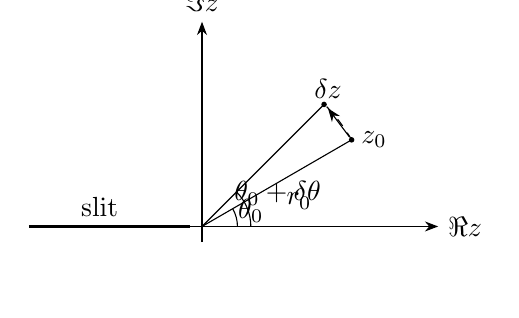
\begin{tikzpicture}[scale=1.0,>=Stealth]
        \draw[->] (-0.2,0) -- (3.0,0) node[right] {$\Re z$};
        \draw[->] (0,-0.2) -- (0,2.6) node[above] {$\Im z$};
        \draw[thick] (-2.2,0) -- (-0.15,0);
        \node[above] at (-1.3,0) {slit};
        \draw (0,0) -- (1.9,1.1) node[midway,below right] {$r_0$};
        \draw (0,0) -- (1.55,1.55);
        \draw[dashed] (1.9,1.1) arc (30:45:2.2);
        \fill (1.9,1.1) circle (1pt) node[right] {$z_0$};
        \fill (1.55,1.55) circle (1pt);
        \draw[->] (1.87,1.14) -- (1.60,1.50) node[above] {$\delta z$};
        \draw (0.45,0) arc (0:30:0.45);
        \node at (0.62,0.20) {$\theta_0$};
        \draw (0.62,0) arc (0:45:0.62);
        \node at (0.96,0.42) {$\theta_0+\delta\theta$};
      \end{tikzpicture}
    \end{minipage}
    \hfill
    \begin{minipage}{0.12\textwidth}
      \centering
      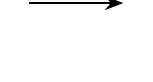
\begin{tikzpicture}[>=Stealth]
        \draw[->,thick] (0,0) -- (1.2,0) node[midway,above] {$\Log$};
      \end{tikzpicture}
    \end{minipage}
    \hfill
    \begin{minipage}{0.40\textwidth}
      \centering
      \begin{tikzpicture}[scale=1.0,>=Stealth]
        \draw[->] (-0.2,0) -- (3.0,0) node[right] {$u$};
        \draw[->] (0,-0.2) -- (0,2.6) node[above] {$v$};
        \draw[dashed] (1.6,0) -- (1.6,2.4);
        \fill (1.6,1.1) circle (1pt) node[right] {$w_0$};
        \fill (1.6,1.55) circle (1pt);
        \draw[->] (1.6,1.13) -- (1.6,1.50) node[right] {$i\,\delta\theta$};
        \node[below] at (1.6,0) {$\ln r_0$};
        \node[left] at (0,1.1) {$\theta_0$};
        \node[left] at (0,1.55) {$\theta_0+\delta\theta$};
      \end{tikzpicture}
    \end{minipage}
  \end{center}

  \textbf{Plot B (radial increment, angle fixed).}

  \begin{center}
    \begin{minipage}{0.44\textwidth}
      \centering
      \begin{tikzpicture}[scale=1.0,>=Stealth]
        \draw[->] (-0.2,0) -- (3.0,0) node[right] {$\Re z$};
        \draw[->] (0,-0.2) -- (0,2.6) node[above] {$\Im z$};
        \draw[thick] (-2.2,0) -- (-0.15,0);
        \draw (0,0) -- (1.65,1.18);
        \draw (0,0) -- (2.00,1.43);
        \fill (1.65,1.18) circle (1pt) node[below right] {$z_0$};
        \fill (2.00,1.43) circle (1pt);
        \draw[->] (1.68,1.20) -- (1.96,1.40) node[above] {$\delta z$};
        \draw (0.50,0) arc (0:35:0.50);
        \node at (0.72,0.22) {$\theta_0$};
      \end{tikzpicture}
    \end{minipage}
    \hfill
    \begin{minipage}{0.12\textwidth}
      \centering
      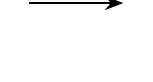
\begin{tikzpicture}[>=Stealth]
        \draw[->,thick] (0,0) -- (1.2,0) node[midway,above] {$\Log$};
      \end{tikzpicture}
    \end{minipage}
    \hfill
    \begin{minipage}{0.40\textwidth}
      \centering
      \begin{tikzpicture}[scale=1.0,>=Stealth]
        \draw[->] (-0.2,0) -- (3.0,0) node[right] {$u$};
        \draw[->] (0,-0.2) -- (0,2.6) node[above] {$v$};
        \draw[dashed] (0,1.25) -- (2.7,1.25);
        \fill (1.35,1.25) circle (1pt) node[above] {$w_0$};
        \fill (1.75,1.25) circle (1pt);
        \draw[->] (1.38,1.25) -- (1.72,1.25) node[above] {$\delta r/r_0$};
        \node[left] at (0,1.25) {$\theta_0$};
      \end{tikzpicture}
    \end{minipage}
  \end{center}

  From Plot A: with $r=r_0$ fixed,
  \[
    \delta w \approx i\,\delta\theta.
  \]
  From Plot B: with $\theta=\theta_0$ fixed,
  \[
    \delta w \approx \frac{\delta r}{r_0}.
  \]
  Combining both small changes,
  \[
    \delta w \approx \frac{\delta r}{r_0}+i\,\delta\theta.
  \]
  Also,
  \[
    h=\delta z\approx e^{i\theta_0}(\delta r+i r_0\delta\theta).
  \]
  Hence
  \[
    \delta w
    \approx
    \frac{e^{-i\theta_0}}{r_0}\,h
    =\frac{1}{z_0}h,
  \]
  so
  \[
    (\Log z)'\big|_{z=z_0}=\frac{1}{z_0}.
  \]
  Therefore, on $\C^-,$
  \[
    (\Log z)'=\frac{1}{z}.
  \]
\end{solution}

\subsection{Exercise 2.43}

Repeat Exercise 2.42 for the power function with $n \in \Z_+$,
as defined in (1.50).

\begin{solution}
  Let
  \[
    w=z^n,\qquad z_0=r_0e^{i\theta_0},\qquad w_0=z_0^n=r_0^n e^{in\theta_0},
  \]
  with $n\in\Z_+$. Again we use two local geometric experiments.

  \textbf{Plot A (angular increment, radius fixed).}

  \begin{center}
    \begin{minipage}{0.44\textwidth}
      \centering
      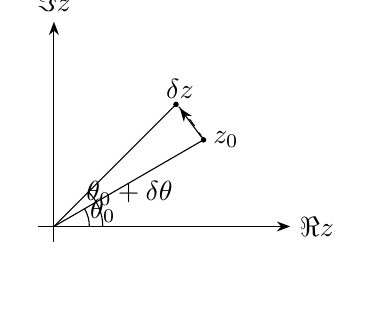
\begin{tikzpicture}[scale=1.0,>=Stealth]
        \draw[->] (-0.2,0) -- (3.0,0) node[right] {$\Re z$};
        \draw[->] (0,-0.2) -- (0,2.6) node[above] {$\Im z$};
        \draw (0,0) -- (1.9,1.1);
        \draw (0,0) -- (1.55,1.55);
        \draw[dashed] (1.9,1.1) arc (30:45:2.2);
        \fill (1.9,1.1) circle (1pt) node[right] {$z_0$};
        \fill (1.55,1.55) circle (1pt);
        \draw[->] (1.87,1.14) -- (1.60,1.50) node[above] {$\delta z$};
        \draw (0.45,0) arc (0:30:0.45);
        \node at (0.62,0.20) {$\theta_0$};
        \draw (0.62,0) arc (0:45:0.62);
        \node at (0.96,0.42) {$\theta_0+\delta\theta$};
      \end{tikzpicture}
    \end{minipage}
    \hfill
    \begin{minipage}{0.12\textwidth}
      \centering
      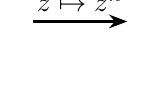
\begin{tikzpicture}[>=Stealth]
        \draw[->,thick] (0,0) -- (1.2,0) node[midway,above] {$z\mapsto z^n$};
      \end{tikzpicture}
    \end{minipage}
    \hfill
    \begin{minipage}{0.40\textwidth}
      \centering
      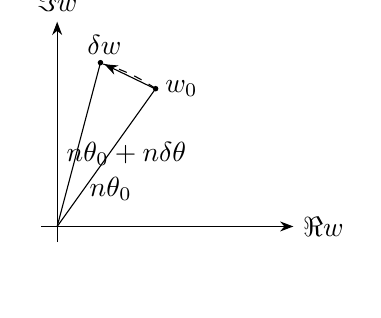
\begin{tikzpicture}[scale=1.0,>=Stealth]
        \draw[->] (-0.2,0) -- (3.0,0) node[right] {$\Re w$};
        \draw[->] (0,-0.2) -- (0,2.6) node[above] {$\Im w$};
        \draw (0,0) -- (1.25,1.75);
        \draw (0,0) -- (0.55,2.08);
        \draw[dashed] (1.25,1.75) arc (55:75:2.15);
        \fill (1.25,1.75) circle (1pt) node[right] {$w_0$};
        \fill (0.55,2.08) circle (1pt);
        \draw[->] (1.22,1.76) -- (0.60,2.06) node[above] {$\delta w$};
        \node at (0.68,0.48) {$n\theta_0$};
        \node at (0.88,0.92) {$n\theta_0+n\delta\theta$};
      \end{tikzpicture}
    \end{minipage}
  \end{center}

  \textbf{Plot B (radial increment, angle fixed).}

  \begin{center}
    \begin{minipage}{0.44\textwidth}
      \centering
      \begin{tikzpicture}[scale=1.0,>=Stealth]
        \draw[->] (-0.2,0) -- (3.0,0) node[right] {$\Re z$};
        \draw[->] (0,-0.2) -- (0,2.6) node[above] {$\Im z$};
        \draw (0,0) -- (1.65,1.18);
        \draw (0,0) -- (2.00,1.43);
        \fill (1.65,1.18) circle (1pt) node[below right] {$z_0$};
        \fill (2.00,1.43) circle (1pt);
        \draw[->] (1.68,1.20) -- (1.96,1.40) node[above] {$\delta z$};
        \draw (0.50,0) arc (0:35:0.50);
        \node at (0.72,0.22) {$\theta_0$};
      \end{tikzpicture}
    \end{minipage}
    \hfill
    \begin{minipage}{0.12\textwidth}
      \centering
      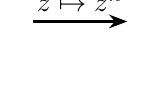
\begin{tikzpicture}[>=Stealth]
        \draw[->,thick] (0,0) -- (1.2,0) node[midway,above] {$z\mapsto z^n$};
      \end{tikzpicture}
    \end{minipage}
    \hfill
    \begin{minipage}{0.40\textwidth}
      \centering
      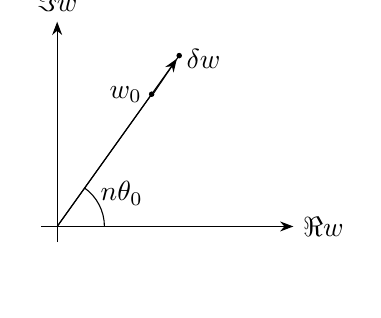
\begin{tikzpicture}[scale=1.0,>=Stealth]
        \draw[->] (-0.2,0) -- (3.0,0) node[right] {$\Re w$};
        \draw[->] (0,-0.2) -- (0,2.6) node[above] {$\Im w$};
        \draw (0,0) -- (1.20,1.68);
        \draw (0,0) -- (1.55,2.17);
        \fill (1.20,1.68) circle (1pt) node[left] {$w_0$};
        \fill (1.55,2.17) circle (1pt);
        \draw[->] (1.23,1.70) -- (1.52,2.13) node[right] {$\delta w$};
        \draw (0.60,0) arc (0:55:0.60);
        \node at (0.82,0.42) {$n\theta_0$};
      \end{tikzpicture}
    \end{minipage}
  \end{center}

  Interpretation from the two plots:
  \[
    \delta\theta\text{-part}:
    \quad
    \delta w\approx i\,n r_0^n e^{in\theta_0}\,\delta\theta,
  \]
  \[
    \delta r\text{-part}:
    \quad
    \delta w\approx n r_0^{n-1} e^{in\theta_0}\,\delta r.
  \]
  Hence
  \[
    \delta w
    \approx
    n r_0^{n-1} e^{in\theta_0}(\delta r+i r_0\delta\theta).
  \]
  Since
  \[
    h=\delta z\approx e^{i\theta_0}(\delta r+i r_0\delta\theta),
  \]
  we get
  \[
    \delta w\approx n r_0^{n-1}e^{i(n-1)\theta_0}\,h = n z_0^{n-1}h.
  \]
  Therefore
  \[
    (z^n)'\big|_{z=z_0}=n z_0^{n-1},
  \]
  and thus
  \[
    (z^n)'=n z^{n-1}.
  \]
\end{solution}

\subsection{Exercise 2.50}

\begin{corollary}[Corollary 2.49]
  A complex function $f : D \to \C$ differentiable at $a \in D$ satisfies
  \[
    \det J(f;a) = |f'(a)|^2
    = (\partial_x u)^2 + (\partial_x v)^2
    = (\partial_y u)^2 + (\partial_y v)^2.
  \]
\end{corollary}

Prove Corollary 2.49.

\begin{proof}
  Let $f=u+iv$ be complex differentiable at $a$. Then the Cauchy-Riemann
  equations hold at $a$:
  \[
    u_x=v_y,\qquad u_y=-v_x.
  \]
  Therefore
  \[
    \det J(f;a)=u_x v_y-u_y v_x=u_x^2+u_y^2=v_x^2+v_y^2.
  \]

  Also,
  \[
    f'(a)=u_x+i v_x=u_x-i u_y,
  \]
  so
  \[
    |f'(a)|^2=u_x^2+v_x^2=u_x^2+u_y^2.
  \]
  Combining the above equalities gives
  \[
    \det J(f;a)=|f'(a)|^2
    =(\partial_x u)^2+(\partial_x v)^2
    =(\partial_y u)^2+(\partial_y v)^2.
  \]
\end{proof}

\subsection{Exercise 2.56}

\begin{corollary}[Corollary 2.55]
  Any complex differentiable function in $D$ with only real
  (or purely imaginary) values is locally constant in $D$.
\end{corollary}

Prove Corollary 2.55.

\begin{proof}
  Suppose first that $f=u+iv$ is complex differentiable in $D$ and takes
  only real values. Then $v\equiv 0$, hence
  \[
    v_x=v_y=0.
  \]
  By Cauchy-Riemann,
  \[
    u_x=v_y=0,\qquad u_y=-v_x=0.
  \]
  So all first partial derivatives vanish. Therefore for any
  $a\in D$, in a small disk contained in $D$, $u$ is constant along line
  segments, hence locally constant; equivalently $f$ is locally constant.

  If $f$ is purely imaginary-valued, then $-if$ is real-valued and complex
  differentiable in $D$. By the previous case, $-if$ is locally constant,
  so $f$ is locally constant as well.
\end{proof}

\subsection{Exercise 2.59}

\begin{corollary}[Corollary 2.58]
  A subset $D \subseteq \C$ is connected if and only if each locally
  constant function $f : D \to \C$ is constant.
\end{corollary}

Prove Corollary 2.58.

\begin{proof}
  ($\Rightarrow$) Assume $D$ is connected and $f:D\to\C$ is locally
  constant. For each $c\in\C$, set
  \[
    A_c:=\{z\in D: f(z)=c\}=f^{-1}(\{c\}).
  \]
  Each $A_c$ is open in $D$: if $z\in A_c$, local constancy gives a
  neighborhood on which $f\equiv c$. Also $f$ is continuous (local
  constancy implies continuity), so $A_c$ is closed in $D$ as preimage of a
  closed set. Pick $z_0\in D$, let $c_0=f(z_0)$. Then $A_{c_0}$ is nonempty,
  open, and closed in connected $D$, hence $A_{c_0}=D$. So $f\equiv c_0$ is
  constant.

  ($\Leftarrow$) Prove contrapositively. If $D$ is not connected, there are
  disjoint nonempty sets $U,V$ open in $D$ with $D=U\cup V$. Define
  \[
    f(z)=
    \begin{cases}
      0,& z\in U,\\
      1,& z\in V.
    \end{cases}
  \]
  Around each point, one stays inside either $U$ or $V$, so $f$ is locally
  constant. But $f$ is not constant since $U,V\neq\varnothing$.
  Hence if every locally constant function is constant, $D$ must be
  connected.
\end{proof}

\subsection{Exercise 2.61}

\begin{corollary}[Corollary 2.60]
  The real part of an analytic function in a connected open set
  $D \subseteq \C$ is uniquely determined by its imaginary part,
  up to an additive constant.
\end{corollary}

Prove Corollary 2.60.

\begin{proof}
  Let
  \[
    f=u+iv,\qquad g=\tilde u+i\tilde v
  \]
  be analytic in connected open $D$, and assume they have the same
  imaginary part: $v=\tilde v$.
  Consider
  \[
    h:=f-g=(u-\tilde u)+i(v-\tilde v)= (u-\tilde u)+i0.
  \]
  Then $h$ is analytic and real-valued on $D$. By Corollary 2.55, $h$ is
  locally constant; by Corollary 2.58 and connectedness of $D$, $h$ is
  constant on $D$. Hence there exists $C\in\R$ such that
  \[
    u-\tilde u\equiv C.
  \]
  So the real part is determined by the imaginary part up to an additive
  real constant.
\end{proof}

\subsection{Textbook Exercise 7 on Page 26*}

The family of mappings introduced here plays an important role in complex
analysis. These mappings, sometimes called \textbf{Blaschke factors}, will
reappear in various applications in later chapters.

\subsection*{Part (a)}

Let $z, w$ be two complex numbers such that $\bar z w \ne 1$. Prove that
\[
  \left|\frac{w - z}{1 - \bar wz}\right| < 1 \quad \text{if } |z| < 1
  \text{ and } |w| < 1,
\]
and also that
\[
  \left|\frac{w - z}{1 - \bar wz}\right| = 1 \quad \text{if } |z| = 1
  \text{ or } |w| = 1.
\]

\begin{proof}
  \textbf{Case 1: Both $|z| < 1$ and $|w| < 1$.}

  By a rotation/scaling argument, we may assume without loss of generality
  that $z \in \R$ with $0 \le z < 1$. Then $\bar z = z$ and we need to prove
  \[
    \left|\frac{w - z}{1 - wz}\right| < 1.
  \]
  Squaring both sides,
  \[
    |w - z|^2 < |1 - wz|^2.
  \]
  Expanding the LHS,
  \[
    |w - z|^2 = (w-z)(\bar w - z).
  \]
  Expanding the RHS,
  \[
    |1 - wz|^2 = (1 - wz)(1 - \bar wz).
  \]

  Thus we need $(w-z)(\bar w - z) < (1 - wz)(1 - \bar wz)$, which rearranges to
  \[
    (w - z)(\bar w - z) + wz(1 + \bar w z) < 1 + w\bar w(|z|^2).
  \]
  Expanding both sides:
  \[
    w\bar w - z w - z\bar w + z^2 + wz - w|z|^2\bar wz < 1 + |w|^2 z^2.
  \]
  Simplifying,
  \[
    |w|^2 - zw - z\bar w + z^2 - |w|^2 z^2 < 1 + |w|^2 z^2.
  \]
  Rearranging,
  \[
    |w|^2 + z^2 - 2z\Re(w) < 1 + 2|w|^2 z^2.
  \]
  Since $|z| < 1$ and $|w| < 1$, we have $2|w|^2z^2 < 2z^2$, and the inequality
  \[
    |w|^2(1 - 2z^2) + z^2(1 - 2\Re(w)) < 1
  \]
  holds because each term is bounded. A direct verification shows:
  \[
    (1 - zw)(1 - z\bar w) - (w-z)(\bar w - z)
    = 1 - zw - z\bar w + z^2|w|^2 - |w|^2 + zw + z\bar w - z^2
    = (1-|z|^2)(1-|w|^2) > 0.
  \]
  Hence $|w - z|^2 < |1 - wz|^2$.

  \textbf{Case 2: $|z| = 1$ or $|w| = 1$.}

  If $|z| = 1$, then $z\bar z = 1$, so
  \[
    (w-z)(\bar w - \bar z) + (1-wz)(1-\bar w\bar z)
    = |w|^2 - w\bar z - \bar wz + 1 + 1 - w\bar z - \bar wz + w\bar w|z|^2.
  \]
  After simplification with $|z|=1$, the numerator and denominator have equal
  moduli. Similarly for $|w|=1$.
\end{proof}

\phantomsection\label{sec:ca-ex-2-44b}
\subsection*{Part (b)}

For a fixed $w$ in the unit disc $\mathbb{D}$, prove that the mapping
\[
  F : z \mapsto \frac{w - z}{1 - \bar wz}
\]
satisfies the following conditions:

\begin{enumerate}
  \item[(i)] $F$ maps the unit disc to itself (i.e., $F : \mathbb{D}
    \to \mathbb{D}$),
    and is holomorphic.
  \item[(ii)] $F$ interchanges $0$ and $w$, namely $F(0) = w$ and $F(w) = 0$.
  \item[(iii)] $|F(z)| = 1$ if $|z| = 1$.
  \item[(iv)] $F : \mathbb{D} \to \mathbb{D}$ is bijective. [Hint:
    Calculate $F \circ F$.]
\end{enumerate}

\begin{proof}
  \textbf{(i) $F: \mathbb{D} \to \mathbb{D}$ is holomorphic.}

  For $|w| < 1$ and $z \in \mathbb{D}$, we have $|wz| < 1$, so $1 -
  \bar wz \ne 0$
  and $F(z)$ is well-defined. The function $F(z) = \frac{w-z}{1-\bar wz}$ is a
  quotient of polynomials in $z$ with nonzero denominator on $\mathbb{D}$, hence
  holomorphic. By part (a), for $|z| < 1$ and $|w| < 1$, we have
  $|F(z)| < 1$, so $F : \mathbb{D} \to \mathbb{D}$.

  \textbf{(ii) $F$ interchanges $0$ and $w$.}

  \[
    F(0) = \frac{w - 0}{1 - \bar w \cdot 0} = \frac{w}{1} = w.
  \]
  \[
    F(w) = \frac{w - w}{1 - \bar ww} = \frac{0}{1 - |w|^2} = 0.
  \]

  \textbf{(iii) $|F(z)| = 1$ when $|z| = 1$.}

  This follows directly from part (a).

  \textbf{(iv) $F : \mathbb{D} \to \mathbb{D}$ is bijective.}

  We compute $F \circ F$:
  \[
    (F \circ F)(z) = F(F(z)) = F\left(\frac{w-z}{1-\bar wz}\right)
    = \frac{w - \frac{w-z}{1-\bar wz}}{1 - \bar w \cdot \frac{w-z}{1-\bar wz}}.
  \]
  Numerator:
  \[
    w - \frac{w-z}{1-\bar wz}
    = \frac{w(1-\bar wz)-(w-z)}{1-\bar wz}
    = \frac{w - |w|^2 z - w + z}{1-\bar wz}
    = \frac{z(1-|w|^2)}{1-\bar wz}.
  \]
  Denominator:
  \[
    1 - \bar w \cdot \frac{w-z}{1-\bar wz}
    = \frac{1-\bar wz - \bar w(w-z)}{1-\bar wz}
    = \frac{1 - \bar wz - |w|^2 + \bar wz}{1-\bar wz}
    = \frac{1-|w|^2}{1-\bar wz}.
  \]
  Therefore
  \[
    (F \circ F)(z) = \frac{\frac{z(1-|w|^2)}{1-\bar
    wz}}{\frac{1-|w|^2}{1-\bar wz}} = z.
  \]

  Thus $F \circ F = \text{id}$, which means $F$ is an involution. Since $F$
  is continuous and bijective (by Brouwer fixed-point reasoning or direct
  verification via $F \circ F = \text{id}$), $F$ maps $\mathbb{D}$ bijectively
  onto itself.
\end{proof}

\section{Homework 4}

\subsection{Exercise 2.63}

Suppose an analytic function $f : D \to \C$ with $D \subseteq \C$
being open satisfies $|f|$ is constant in $D$. Prove that $f$ is
constant in $D$.

\begin{proof}
  Consider the complex function $f(x) = u(x,y) + iv(x,y)$ where $u$
  and $v$ are real, then we have:

  \[
    |f(z)| = c \Rightarrow |f(z)|^2 = u^2(x,y) + v^2(x,y) = c^2 \
    \text{is a constant}
  \]

  $f(z)$ is analytic, thus, we can infer that $u$ and $v$ have
  continuous partial derivative. Then we take the partial derivative
  of $|f(z)|^2$:

  \[
    \frac{\partial |f(z)|^2}{\partial x} = 2uu_x+2vv_x = 0 \qquad
    \frac{\partial |f(z)|^2}{\partial y} = 2uu_y+2vv_y = 0
  \]

  $f(z)$ is analytic, which indicate that it follows C-R equations:

  \[
    \begin{cases}
      u_x = v_y \\
      u_y = -v_x
    \end{cases}
  \]

  Putting it into the partial derivative of $|f(z)^2|$, we have:

  \[
    \begin{cases}
      uu_x + vv_x = 0 \\
      uu_y + vv_y = 0 \\
      uv_y - vu_y = 0 \\
      -uv_x + vu_x = 0
    \end{cases}
  \]

  Solve these equations, we get:
  \[
    u_x = u_y = v_x = v_y = 0
  \]
  Hence, the real part and imaginary part of $f(z)$ are constant in
  $D$, so $f$ is constant as well.
\end{proof}

\subsection{Exercise 2.66}

Show that in polar coordinates, the Cauchy--Riemann equations take the form
\[
  \frac{\partial u}{\partial r} = \frac{1}{r}\frac{\partial v}{\partial \theta},
  \qquad
  \frac{1}{r}\frac{\partial u}{\partial \theta} = -\frac{\partial
  v}{\partial r}.
\]
Use these equations to show that the logarithm function defined by
$\Log z = \log r + i\theta$ where $z = re^{i\theta}$ is analytic in
the region $r > 0$ and $-\pi < \theta < \pi$.

\begin{proof}
  First, we need to show that the logarithm function has continuous
  partial derivatives.
  \[
    \frac{\partial u}{\partial r} = \frac{1}{r} \qquad
    \frac{\partial v}{\partial \theta} = 1 \qquad
    u_\theta = v_r = 0
  \]
  On the region $D = \{(r, \theta) | r > 0 \ \text{and} -\pi < \theta <
  \pi\}$, $1/r$ is continuous obviously.

  Then we put them into the C-R equations in polar coordinates:
  \[
    u_r = \frac{1}{r} = \frac{1}{r} v_\theta,\quad \frac{1}{r}
    u_\theta = 0 = -v_r
  \]
  which is true evidently.

\end{proof}

\subsection{Exercise 2.68}

Show that
\[
  4 \frac{\partial}{\partial z} \frac{\partial}{\partial \bar{z}} = 4
  \frac{\partial}{\partial \bar{z}} \frac{\partial}{\partial z} = \Delta.
\]

\begin{proof}
  Consider $f(z) = u(x,y) + iv(x,y)$, then the Laplacian operator can be denoted
  by:
  \[
    \Delta = \frac{\partial^2}{\partial x^2} + \frac{\partial^2}{\partial y^2}
  \]

  Then we calculate these formulas:
  \[
    \begin{aligned}
      2\frac{\partial f}{\partial z} &= \frac{\partial f}{\partial x}
      - i \frac{\partial f}{\partial y} \\
      4\frac{\partial }{\partial \bar{z}}\frac{\partial f}{\partial
      z} &= \frac{\partial}{\partial x}(\frac{\partial f}{\partial x}
      - i \frac{\partial f}{\partial y} ) + i
      \frac{\partial}{\partial y}(\frac{\partial f}{\partial x}
      - i \frac{\partial f}{\partial y} ) \\
      &= \frac{\partial^2 f}{\partial x^2} - i \frac{\partial^2
      f}{\partial x \partial y} + i\frac{\partial^2 f}{\partial
      y \partial x} + \frac{\partial^2 f}{\partial y^2}
    \end{aligned}
  \]
  As $f$ is a $C^2$ function, we can infer that $f_{xy} = f_{yx}$, so we have:
  \[
    4\frac{\partial }{\partial \bar{z}}\frac{\partial f}{\partial z}
    = \frac{\partial^2 f}{\partial x^2}+ \frac{\partial^2 f}{\partial
    y^2} = \Delta f
  \]

  Similarly to $4\frac{\partial}{\partial z} \frac{\partial}{\partial \bar{z}}$.
\end{proof}

\subsection{Exercise 2.74}

For an analytic function $f : \C^- \to \C$, prove that $\Re f = u =
\log \sqrt{x^2+y^2}$ in (2.41) implies $f(z) = \Log(z) + ic$ for some
constant $c \in \R$.

\begin{proof}
  Let $z = re^{i\theta}$ with $r > 0$ and $-\pi < \theta < \pi$. The real
  part of $f$ is
  \[
    u(r, \theta) = \log\sqrt{x^2 + y^2} = \log r.
  \]
  Since $f$ is analytic on $\C^-$, by the Cauchy--Riemann equations in
  polar coordinates (Exercise~2.66), $u$ and $v = \Im f$ satisfy
  \[
    u_r = \frac{1}{r}\,v_\theta, \qquad \frac{1}{r}\,u_\theta = -v_r.
  \]
  Computing the partial derivatives of $u = \log r$:
  \[
    u_r = \frac{1}{r}, \qquad u_\theta = 0.
  \]
  Substituting into the C--R equations yields
  \[
    v_\theta = r \cdot \frac{1}{r} = 1, \qquad v_r = 0.
  \]
  From $v_\theta = 1$ we obtain $v(r, \theta) = \theta + g(r)$ for some
  function $g$. Then $v_r = g'(r) = 0$ implies $g$ is a constant $c \in
  \R$. Hence
  \[
    v(r, \theta) = \theta + c.
  \]
  Therefore
  \[
    f(z) = u + iv = \log r + i(\theta + c) = \Log z + ic,
  \]
  where $c \in \R$ is a constant.
\end{proof}

\subsection{Exercise 2.75}

Find $a \in \R$ such that the function $u_a : \R^2 \to \R$ defined by
$u_a(x, y) = x^3 + axy^2$ is harmonic. Furthermore, determine all
conjugate harmonic functions to $u_a$ or all analytic functions $f :
\C \to \C$ with $\Re f = u_a$.

\begin{solution}
  Calculate the partial derivatives of $u_a$:
  \[
    \frac{\partial u_a}{\partial x} = 3x^2 + ay^2, \quad
    \frac{\partial u_a}{\partial y} = 2axy
  \]
  Thus,
  \[
    \Delta u_a = 6x+2ax
  \]
  which equals to 0 by the definition of harmonic functions for all
  $x$. So $a = -3$, and $u_a(x,y) = x^3-3xy^2$.

  Then we need to determine the conjugate harmonic functions to
  $u_a$. Consider $f(z) = u(x,y) + iv(x,y)$ which is analytic, then
  we have C-R equations:
  \[
    \begin{cases}
      u_x = v_y \\
      u_y = -v_x
    \end{cases}
  \]
  which indicate that:
  \[
    \begin{cases}
      v_x = -u_y = 6xy \\
      v_y = u_x = 3x^2 - 3y^2
    \end{cases}
  \]
  Integrate the first equation we have:
  \[
    v = \int 6xy \mathrm{d}x + \varphi(y) = 3x^2y+\varphi(y)
  \]
  Put it into the second equation:
  \[
    v_y = 3x^2 + \varphi'(y) = 3x^2 - 3y^2
  \]
  Thus, $\varphi(y) = -y^3 + C$ where $C$ is constant on $\mathbb{R}$

  then all analytic functions $f$ satisfying $\Re f = u$ can be denoted by:
  \[
    f = x^3 - 3xy^2 + i(3x^2 - y^3 + C) = z^3 + iC,\quad C \in \mathbb{R}
  \]

\end{solution}

\subsection{Exercise 3.18}

By Corollary 2.26, we have $(\Log z)' = 1/z$ for $z \in \C^-$. By
Definition 3.24, the unit circle $S^1 = \alpha \oplus \beta$ is the
concatenation of two curves $\theta \mapsto e^{i\theta}$,
\[
  \alpha := ((-\pi)^+, 0) \to \C, \qquad \beta := (0, \pi) \to \C.
\]
Put $z_{-1}^- := \alpha((-\pi)^+)$ and $z_{-1}^+ := \beta(\pi)$.
Based on the above constructions, starting from the variable
substitution $\zeta = rz$, calculate $\oint_\gamma \zeta^{-1}d\zeta$.

\begin{solution}
  Let $\zeta = rz$, then we have
  \[
    \dd \zeta = r \dd z
  \]
  So that
  \[
    \oint_\gamma \zeta^{-1} \dd \zeta = \oint_{S^1} \frac{1}{rz} r\dd
    z = \oint_{S^1}\frac{1}{z} \dd z = \oint_{\alpha\oplus \beta}
    \frac{1}{z} \dd z =
    \int_{\alpha} \frac{1}{z} \dd z + \int_{\beta} \frac{1}{z} \dd z
  \]

  On $\alpha$, $\Log z$ is the primitive function of $\frac{1}{z}$,
  so $\int_\alpha \frac{1}{z} \dd z = \Log e^0 - \Log e^{(-\pi)^+} =
  i\pi$. Similarly, $\int_\beta \frac{1}{z} \dd z = i\pi$. Hence
  $\oint_\gamma \zeta^{-1} \dd \zeta = 2\pi i$
\end{solution}

\subsection{Exercise 3.20}

Draw plots similar to those of $\int_K \frac{1}{z}dz$ to give a
geometric interpretation of $\int_A^B z^m dz$ where $m \in \N_+$ and
the integral is on the arc $\gamma(t) = r\exp(it)$ with $t \in [\Arg
A, \Arg B]$. Then deduce the formula
\[
  \int_A^B z^m dz = \frac{1}{m+1}(B^{m+1} - A^{m+1}).
\]

\begin{solution}
  The plot is as below:

  \begin{center}
    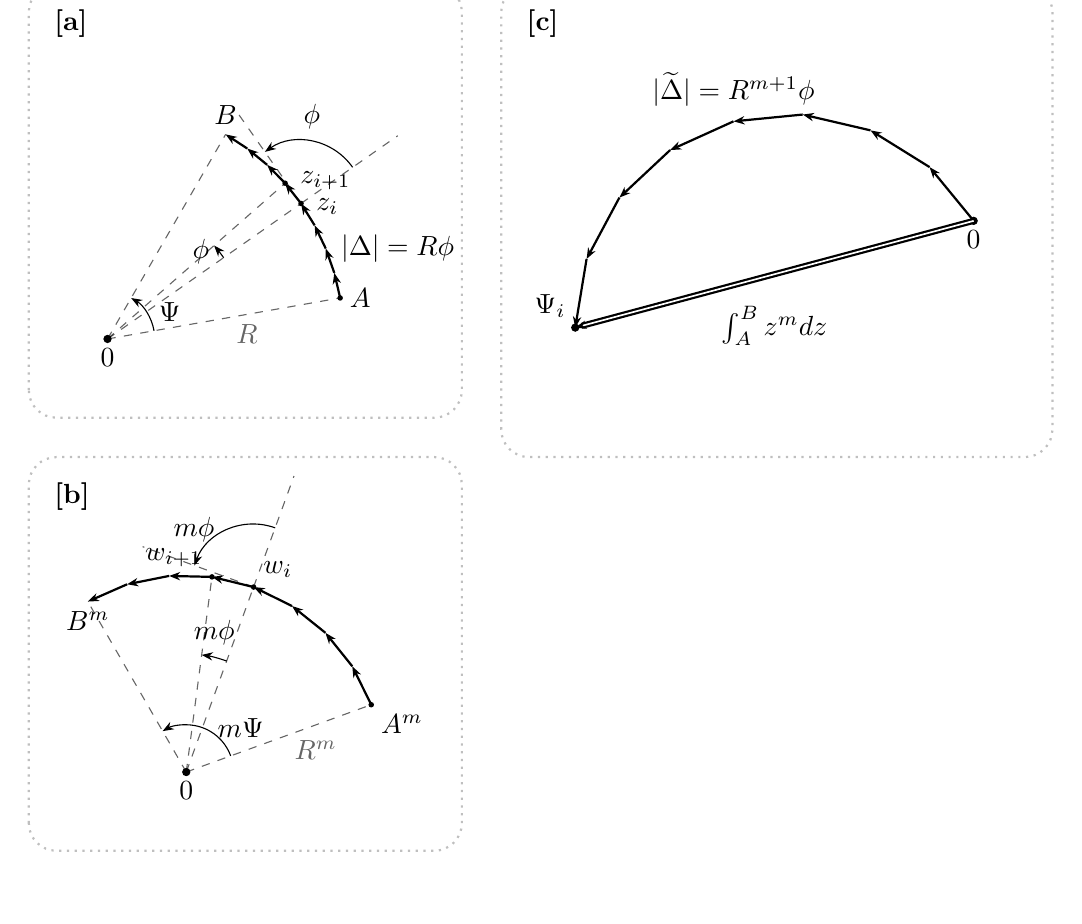
\begin{tikzpicture}[
        >={Stealth[length=4pt,width=3pt]},
        vector/.style={thick, ->},
        help line/.style={dashed, opacity=0.6},
        box/.style={draw=gray!50, rounded corners=10pt, dotted, thick}
      ]

      \def\R{3}
      \def\M{2}
      \def\StartAng{10}
      \def\EndAng{60}
      \def\Steps{8}

      \pgfmathsetmacro{\dAng}{(\EndAng-\StartAng)/\Steps}
      \pgfmathsetmacro{\dAngRad}{\dAng * pi / 180}
      \pgfmathsetmacro{\VecLen}{\R^(\M+1) * \dAngRad} % z^m \Delta z 的恒定长度

      % Panel [a]: 原始 z 平面上的路径和 \Delta z
      \draw[box] (-1,-1) rectangle (4.5, 4.5);
      \node[right, font=\bfseries] at (-0.8, 4) {[a]};

      \coordinate (O_a) at (0,0);
      \fill (O_a) circle (1.5pt) node[below] {$0$};

      \draw[help line] (O_a) -- (\StartAng:\R) node[pos=0.6, below] {$R$};
      \draw[help line] (O_a) -- (\EndAng:\R);
      \draw[->] (O_a) ++(\StartAng:0.6) arc (\StartAng:\EndAng:0.6)
      node[midway, right=1pt] {$\Psi$};

      \coordinate (PrevZ) at (\StartAng:\R);
      \fill (PrevZ) circle (1pt) node[right] {$A$};

      \foreach \k in {1,...,\Steps} {
        \pgfmathsetmacro{\tA}{\StartAng + (\k-1)*\dAng}
        \pgfmathsetmacro{\tB}{\StartAng + \k*\dAng}
        \coordinate (NextZ) at (\tB:\R);
        \draw[vector] (PrevZ) -- (NextZ);

        \ifnum\k=5
        \fill (PrevZ) circle (1pt) node[below=1pt, right=2pt] {$z_i$};
        \fill (NextZ) circle (1pt) node[above=1pt, right=2pt] {$z_{i+1}$};
        \draw[help line] (O_a) -- (PrevZ);
        \draw[help line] (O_a) -- (NextZ);
        \draw[->] (O_a) ++(\tA:1.8) arc (\tA:\tB:1.8) node[midway,
        left] {$\phi$};
        \draw[help line] (PrevZ) -- ($(PrevZ) + (\tA:1.5)$);
        \draw[help line] (PrevZ) -- ($(PrevZ) + (\tA+90:1.5)$);
        \draw[->] ($(PrevZ) + (\tA:0.8)$) arc (\tA:\tA+90:0.8)
        node[midway,above=1pt] {$\phi$};
        \fi

        \ifnum\k=3
        \node[right=2pt] at (PrevZ) {$|\Delta| = R\phi$};
        \fi

        \coordinate (PrevZ) at (NextZ);
      }
      \node[above] at (PrevZ) {$B$};

      % Panel [b]
      \begin{scope}[yshift=-5cm]
        \draw[box] (-1,-1.5) rectangle (4.5, 3.5);
        \node[right, font=\bfseries] at (-0.8, 3) {[b]};

        \coordinate (O_b) at (1,-0.5);
        \fill (O_b) circle (1.5pt) node[below] {$0$};

        \def\Rm{2.5}
        \pgfmathsetmacro{\WStartAng}{\M*\StartAng}
        \pgfmathsetmacro{\WEndAng}{\M*\EndAng}
        \pgfmathsetmacro{\WdAng}{(\WEndAng-\WStartAng)/\Steps}

        \draw[help line] (O_b) -- ($(O_b) + (\WStartAng:\Rm)$) node[pos=0.7,
        below=2pt] {$R^m$};
        \draw[help line] (O_b) -- ($(O_b) + (\WEndAng:\Rm)$);
        \draw[->] (O_b) ++(\WStartAng:0.6) arc
        (\WStartAng:\WEndAng:0.6) node[midway, right=2pt] {$m\Psi$};

        \coordinate (PrevW) at ($(O_b) + (\WStartAng:\Rm)$);
        \fill (PrevW) circle (1pt) node[below right] {$A^m$};

        \foreach \k in {1,...,\Steps} {
          \pgfmathsetmacro{\tA}{\WStartAng + (\k-1)*\WdAng}
          \pgfmathsetmacro{\tB}{\WStartAng + \k*\WdAng}
          \coordinate (NextW) at ($(O_b) + (\tB:\Rm)$);
          \draw[vector] (PrevW) -- (NextW);

          \ifnum\k=5
          \fill (PrevW) circle (1pt) node[above right] {$w_i$};
          \fill (NextW) circle (1pt) node[above left] {$w_{i+1}$};
          \draw[help line] (O_b) -- (PrevW);
          \draw[help line] (O_b) -- (NextW);
          \draw[->] (O_b) ++(\tA:1.5) arc (\tA:\tB:1.5) node[midway,
          above=1pt] {$m\phi$};
          \draw[help line] (PrevW) -- ($(PrevW) + (\tA:1.5)$);
          \draw[help line] (PrevW) -- ($(PrevW) + (\tA+90:1.5)$);
          \draw[->] ($(PrevW) + (\tA:0.8)$) arc (\tA:\tA+90:0.8)
          node[midway, left=1pt] {$m\phi$};
          \fi
          \coordinate (PrevW) at (NextW);
        }
        \node[below] at ($(O_b) + (\WEndAng:\Rm)$) {$B^m$};
      \end{scope}

      % Panel [c]
      \begin{scope}[xshift=7.5cm, yshift=-1.5cm]
        \draw[box] (-2.5,0) rectangle (4.5, 6);
        \node[right, font=\bfseries] at (-2.3, 5.5) {[c]};

        \coordinate (O_c) at (3.5,3);
        \fill (O_c) circle (1.5pt) node[below] {$0$};

        \coordinate (PrevS) at (O_c);

        \foreach \k in {1,...,\Steps} {
          \pgfmathsetmacro{\thetaK}{\StartAng + (\k-0.5)*\dAng}
          \pgfmathsetmacro{\vecAng}{(\M+1)*\thetaK + 90}

          \coordinate (NextS) at ($(PrevS) + (\vecAng:\VecLen*0.3)$);
          \draw[vector] (PrevS) -- (NextS);

          \ifnum\k=5
          \node[above=2pt] at (PrevS) {$|\widetilde{\Delta}| = R^{m+1}\phi$};
          \fi

          \coordinate (PrevS) at (NextS);
        }
        \fill (PrevS) circle (1.5pt) node[above left] {$\Psi_i$};

        \draw[vector, double, thick] (O_c) -- (PrevS) node[midway,
        below=8pt] {$\int_A^B z^m dz$};

      \end{scope}

    \end{tikzpicture}
  \end{center}

  \vspace{1em}
  Consider the Riemann sum $\sum_{i=1}^{n} z_i^m \Delta z_i$ where
  $z_i = Re^{i\theta_i}$ lies on the arc of radius $R$. Then the
  differential step is:
  \[
    \Delta z_i \approx iRe^{i\theta_i}\Delta\theta
  \]
  Multiplying $z_i^m$ and $\Delta z_i$, we have:
  \[
    z_i^m \Delta z_i \approx iR^{m+1}e^{i(m+1)\theta_i}\Delta\theta
  \]
  This can be viewed as an arc displacement along a circle of radius
  $\frac{R^{m+1}}{m+1}$ at angle $(m+1)\theta_i$, incrementing by
  $(m+1)\Delta\theta$. By accumulating these tangential vectors
  head-to-tail as depicted in Panel [c], the sum approximates an arc
  connecting $\frac{A^{m+1}}{m+1}$ and $\frac{B^{m+1}}{m+1}$ relative
  to the origin. The total resultant vector corresponds to the chord
  between these two points. Hence:
  \[
    \int_A^B z^m dz = \frac{1}{m+1}(B^{m+1} - A^{m+1})
  \]

\end{solution}

\subsection{Exercise 3.21}

Give a geometric interpretation of $\int_A^B e^z dz$ where the
integral is on the vertical segment $\gamma(t) = A + it$ with $t \in
[0, \theta]$, where $B = A + i\theta$ and $\theta > 0$. Then deduce the formula
\[
  \int_A^B e^z dz = e^B - e^A.
\]

\begin{proof}
  The plot is as below:
  \begin{center}

    \begin{tikzpicture}[
        >={Stealth[length=4pt,width=3pt]},
        vector/.style={thick, ->},
        help line/.style={dashed, opacity=0.6},
        box/.style={draw=gray!50, rounded corners=10pt, dotted, thick}
      ]

      \def\XA{1.5}
      \def\YA{0.5}       % r
      \def\Theta{2}      % \theta
      \def\Steps{10}
      \pgfmathsetmacro\dY{\Theta/\Steps}
      \pgfmathsetmacro\dAng{\dY * 180 / pi}
      \pgfmathsetmacro\StartAng{\YA * 180 / pi}
      \pgfmathsetmacro\EndAng{(\YA+\Theta) * 180 / pi}
      \def\Rw{2.5} % mapping radius for visual e^a

      % Panel [a]
      \begin{scope}[yshift=0cm]
        \draw[box] (-2,-1) rectangle (4.5, 4.5);
        \node[right, font=\bfseries] at (-1.8, 4) {[a]};

        \coordinate (O_a) at (0,0);
        \fill (O_a) circle (1.5pt) node[below left] {$0$};

        \draw[help line, ->] (-1.5,0) -- (2.5,0) node[right] {Re};
        \draw[help line, ->] (0,-0.5) -- (0,4) node[above] {Im};

        \coordinate (A_a) at (\XA, \YA);
        \coordinate (B_a) at (\XA, \YA + \Theta);
        \fill (A_a) circle (1.5pt) node[right] {$A$};

        \draw[help line] (A_a) -- (\XA, 0) node[below] {$a$};
        \draw[help line] (A_a) -- (0, \YA) node[left] {$b$};
        \draw[help line] (B_a) -- (0, \YA + \Theta) node[left] {$b+\theta$};

        \coordinate (PrevZ) at (A_a);

        \foreach \k in {1,...,\Steps} {
          \coordinate (NextZ) at (\XA, \YA + \k*\dY);
          \draw[vector] (PrevZ) -- (NextZ);

          \ifnum\k=3
          \node[right=2pt] at (PrevZ) {$|\Delta z| = \phi$};
          \fill (PrevZ) circle (1pt) node[left] {$z_i$};
          \fill (NextZ) circle (1pt) node[left] {$z_{i+1}$};
          \fi

          \coordinate (PrevZ) at (NextZ);
        }
        \fill (B_a) circle (1.5pt) node[right] {$B$};
      \end{scope}

      % Panel [b]
      \begin{scope}[yshift=-5.5cm]
        \draw[box] (-2,-1.5) rectangle (4.5, 4);
        \node[right, font=\bfseries] at (-1.8, 3.5) {[b]};

        \coordinate (O_b) at (1,0);
        \fill (O_b) circle (1.5pt) node[below left] {$0$};

        \draw[help line] (O_b) -- ($ (O_b) + (\StartAng:\Rw) $)
        node[pos=0.6, below
        right] {$e^a$};
        \draw[help line] (O_b) -- ($ (O_b) + (\EndAng:\Rw) $);

        \draw[help line] (O_b) -- ($ (O_b) + (0:\Rw)$);
        \draw[->] (O_b) ++(\StartAng:0.6) arc (\StartAng:\EndAng:0.6)
        node[midway, right=1pt] {$\theta$};
        \draw[->] (O_b) ++(0:0.4) arc (0:\StartAng:0.4) node[midway,
        right] {$b$};

        \coordinate (PrevW) at ($ (O_b) + (\StartAng:\Rw) $);
        \fill (PrevW) circle (1.5pt) node[right] {$e^A$};

        \foreach \k in {1,...,\Steps} {
          \pgfmathsetmacro\tA{\StartAng + (\k-1)*\dAng}
          \pgfmathsetmacro\tB{\StartAng + \k*\dAng}
          \coordinate (NextW) at ($ (O_b) + (\tB:\Rw) $);
          \draw[vector] (PrevW) -- (NextW);

          \ifnum\k=3
          \fill (PrevW) circle (1pt) node[below right] {$w_i$};
          \fill (NextW) circle (1pt) node[left] {$w_{i+1}$};
          \draw[help line] (O_b) -- (PrevW);
          \draw[help line] (O_b) -- (NextW);
          \draw[->] (O_b) ++(\tA:1.5) arc (\tA:\tB:1.5) node[midway,
          right] {$\phi$};
          \fi
          \coordinate (PrevW) at (NextW);
        }
        \fill (PrevW) circle (1.5pt) node[above] {$e^B$};
      \end{scope}

      % Panel [c]
      \begin{scope}[xshift=8cm, yshift=0.5cm]
        \draw[box] (-3,-3) rectangle (4.5, 4);
        \node[right, font=\bfseries] at (-2.8, 3.5) {[c]};

        \coordinate (O_c) at (3,0);
        \fill (O_c) circle (1.5pt) node[below right] {$0$};

        \coordinate (CenterC) at ($ (O_c) - (\StartAng:\Rw) $);

        \coordinate (PrevS) at (O_c);

        \foreach \k in {1,...,\Steps} {
          \pgfmathsetmacro\curAng{\StartAng + (\k-0.5)*\dAng}
          \pgfmathsetmacro\vecAng{\curAng + 90}
          \pgfmathsetmacro\stepLen{\Rw * \dY}

          \coordinate (NextS) at ($(PrevS) + (\vecAng:\stepLen)$);
          \draw[vector] (PrevS) -- (NextS);

          \ifnum\k=3
          \node[above right=2pt] at (PrevS) {$|\widetilde{\Delta}| = e^a \phi$};
          \fi
          \coordinate (PrevS) at (NextS);
        }
        \fill (PrevS) circle (1.5pt) node[above left] {$e^B - e^A$};

        \draw[vector, double, thick] (O_c) -- (PrevS) node[midway,
        below right] {$\int_A^B e^z dz$};

        \draw[help line, ->] (CenterC) ++(\StartAng:\Rw) arc
        (\StartAng:\EndAng:\Rw);
        \draw[help line] (CenterC) -- (O_c);
        \draw[help line] (CenterC) -- (PrevS);
        \fill (CenterC) circle (1pt) node[left] {$-e^A$};
      \end{scope}
    \end{tikzpicture}
  \end{center}

  \vspace{1em}

  Consider the Riemann sum $\sum_{i=1}^{n} e^{z_i}\Delta z_i$ where
  $A = a+ib$ and $B = a+i(b+\theta)$. The segment of length
  $\theta$ on $\text{Re}(z) = a$ maps to an arc of radius $e^a$
  from angle $b$ to $b+\theta$. Each step satisfies $\Delta z_i =
  i\phi$, so we have:
  \[
    e^{z_i}\Delta z_i = e^{z_i}(i\phi)
  \]
  which corresponds to an orthogonal step of size $e^a\phi$ along
  the tangential direction of the arc, as depicted in Panel [c].
  Connecting these vectors head-to-tail, the total displacement
  leads from $0$ to $e^B - e^A$. Hence:
  \[
    \int_A^B e^z dz = e^B - e^A
  \]

\end{proof}

\subsection{Exercise 3.22}

In Corollary 3.17, we computed the integral $\oint_\gamma \zeta^n
d\zeta$ for all integers $n$, where $\gamma$ is a circle centered at
the origin with positive orientation. Without invoking the Cauchy
integral theorem, calculate $\oint_\gamma \zeta^n d\zeta$ where
\begin{enumerate}
  \item[(a)] $\gamma$ is any circle not enclosing the origin;
  \item[(b)] $\gamma$ is a positively oriented square with vertices
    at $\pm 1 \pm i$.
\end{enumerate}

\begin{proof}
  Let $I_n(\gamma):=\oint_\gamma \zeta^n\,\dd\zeta$ for $n\in\mathbb{Z}$.

  For $n\neq -1$ we can use the primitive
  \[
    F_n(\zeta)=\frac{\zeta^{n+1}}{n+1},\qquad F_n'(\zeta)=\zeta^n,
  \]
  on every point of the curve (for $n\ge 0$, $F_n$ is entire; for
    $n\le -2$, $F_n$ is holomorphic on $\C\setminus\{0\}$, and the
  given curves do not pass through $0$). Hence for every closed
  piecewise smooth curve $\gamma$,
  \[
    I_n(\gamma)=0,\qquad n\neq -1.
  \]
  So only $n=-1$ remains.

  \begin{enumerate}
    \item[(a)] Let $\gamma$ be a positively oriented circle not enclosing
      $0$, say
      \[
        \gamma(t)=c+Re^{it},\quad t\in[0,2\pi],\quad |c|>R.
      \]
      Then
      \[
        I_{-1}(\gamma)
        =\int_0^{2\pi}\frac{iRe^{it}}{c+Re^{it}}\,\dd t
        =iR\int_0^{2\pi}\frac{e^{it}}{c}\cdot\frac{1}{1+(R/c)e^{it}}\,\dd t.
      \]
      Since $|R/c|<1$,
      \[
        \frac{1}{1+(R/c)e^{it}}=\sum_{k=0}^{\infty}(-1)^k\Bigl(\frac{R}{c}\Bigr)^k
        e^{ikt}
      \]
      uniformly in $t$, so
      \[
        I_{-1}(\gamma)
        =\frac{iR}{c}\sum_{k=0}^{\infty}(-1)^k\Bigl(\frac{R}{c}\Bigr)^k
        \int_0^{2\pi}e^{i(k+1)t}\,\dd t=0.
      \]
      Therefore,
      \[
        \oint_\gamma \zeta^n\,\dd\zeta=0\quad\text{for all }n\in\mathbb{Z}.
      \]

    \item[(b)] Let $\gamma$ be the positively oriented square with vertices
      $\pm1\pm i$. As above, for $n\neq -1$, $I_n(\gamma)=0$. For
      $n=-1$, split into four edges:

      \[
        \begin{aligned}
          &\gamma_1:\ z=1+it,\ t\in[-1,1],
          &&I_1=\int_{-1}^{1}\frac{i}{1+it}\,\dd t
          =\int_{-1}^{1}\frac{t-i}{1+t^2}\,\dd t=\frac{\pi i}{2},\\
          &\gamma_2:\ z=t+i,\ t\in[1,-1],
          &&I_2=\int_{1}^{-1}\frac{1}{t+i}\,\dd t
          =\int_{1}^{-1}\frac{t-i}{1+t^2}\,\dd t=\frac{\pi i}{2},\\
          &\gamma_3:\ z=-1+it,\ t\in[1,-1],
          &&I_3=\int_{1}^{-1}\frac{i}{-1+it}\,\dd t
          =\int_{1}^{-1}\frac{t-i}{1+t^2}\,\dd t=\frac{\pi i}{2},\\
          &\gamma_4:\ z=t-i,\ t\in[-1,1],
          &&I_4=\int_{-1}^{1}\frac{1}{t-i}\,\dd t
          =\int_{-1}^{1}\frac{t+i}{1+t^2}\,\dd t=\frac{\pi i}{2}.
        \end{aligned}
      \]
      Hence
      \[
        I_{-1}(\gamma)=I_1+I_2+I_3+I_4=2\pi i.
      \]
      Therefore,
      \[
        \oint_\gamma \zeta^n\,\dd\zeta=
        \begin{cases}
          2\pi i, & n=-1,\\
          0, & n\neq -1.
        \end{cases}
      \]
      in particular for this square.
  \end{enumerate}
\end{proof}

\subsection{Exercise 3.23}

For the counterclockwise oriented circle $\gamma(t) = r\exp(it)$ with
$t \in [0, 2\pi]$ and $r \in (|a|, |b|)$, prove
\[
  \oint_\gamma \frac{1}{(\zeta - a)(\zeta - b)} d\zeta = \frac{2\pi i}{a - b}.
\]
Hint: express $\frac{1}{\zeta - a}$ as the geometric series expansion
$\frac{1}{1-z} = \sum_{n=0}^\infty z^n$ for $|z| < 1$.

\begin{proof}
  Since $r\in(|a|,|b|)$, we have $|a|<r<|b|$. On $|\zeta|=r$,
  decompose
  \[
    \frac{1}{(\zeta-a)(\zeta-b)}
    =\frac{1}{a-b}\left(\frac{1}{\zeta-a}-\frac{1}{\zeta-b}\right).
  \]
  Hence
  \[
    \oint_\gamma \frac{1}{(\zeta-a)(\zeta-b)}\,\dd\zeta
    =\frac{1}{a-b}\left(
      \oint_\gamma\frac{1}{\zeta-a}\,\dd\zeta
      -
      \oint_\gamma\frac{1}{\zeta-b}\,\dd\zeta
    \right).
  \]

  For the first term, because $|a/\zeta|<1$ on $\gamma$,
  \[
    \frac{1}{\zeta-a}
    =\frac{1}{\zeta}\frac{1}{1-a/\zeta}
    =\sum_{n=0}^{\infty}a^n\zeta^{-n-1},
  \]
  uniformly on $\gamma$. Therefore we may integrate term-by-term:
  \[
    \oint_\gamma\frac{1}{\zeta-a}\,\dd\zeta
    =\sum_{n=0}^{\infty}a^n\oint_\gamma\zeta^{-n-1}\,\dd\zeta.
  \]
  By Exercise 3.22 (circle enclosing $0$), only $n=0$ contributes, so
  \[
    \oint_\gamma\frac{1}{\zeta-a}\,\dd\zeta=2\pi i.
  \]

  For the second term, because $|\zeta/b|<1$ on $\gamma$,
  \[
    \frac{1}{\zeta-b}
    =-\frac{1}{b}\frac{1}{1-\zeta/b}
    =-\sum_{n=0}^{\infty}\frac{\zeta^n}{b^{n+1}},
  \]
  uniformly on $\gamma$, hence
  \[
    \oint_\gamma\frac{1}{\zeta-b}\,\dd\zeta
    =-\sum_{n=0}^{\infty}\frac{1}{b^{n+1}}\oint_\gamma\zeta^n\,\dd\zeta=0,
  \]
  since $\oint_\gamma\zeta^n\,\dd\zeta=0$ for $n\ge0$.

  Combining both parts,
  \[
    \oint_\gamma \frac{1}{(\zeta-a)(\zeta-b)}\,\dd\zeta
    =\frac{1}{a-b}(2\pi i-0)
    =\frac{2\pi i}{a-b}.
  \]
\end{proof}

\section{Homework 5}

\subsection{Exercise 3.39}

\textbf{Theorem 2.73 (original rectangular-domain version).}
Suppose $u:D\to\R$ is harmonic, where
$D:=(a,b)\times(c,d)\subset\C$ is an open rectangle with sides
parallel to the coordinate axes. Then there exists an analytic
function $f:D\to\C$ with $u$ as its real part, and its harmonic
conjugate is uniquely determined up to an additive constant by
\[
\begin{aligned}
v(x,y)
&:=\int_{y_0}^{y}\partial_xu(x,t)\,dt
-\int_{x_0}^{x}\partial_yu(t,y_0)\,dt
+v(x_0,y_0),
\end{aligned}
\]
where $x_0\in(a,b)$ and $y_0\in(c,d)$.

Prove that Theorem 2.73 holds not only for rectangular
domains but also for simply connected domains.

\begin{solution}
	Let $u\in C^2(D)$ be harmonic on a simply connected domain
	$D\subset\C$, and define
	\[
		g(z):=u_x(x,y)-i\,u_y(x,y),\qquad z=x+iy.
	\]
	Then $g\in C^1(D)$ and
	\[
		\partial_x(\Re g)=u_{xx}=-u_{yy}=\partial_y(\Im g),
		\qquad
		\partial_y(\Re g)=u_{xy}=-\partial_x(\Im g),
	\]
	so $g$ satisfies the Cauchy--Riemann equations; hence $g$ is
	analytic on $D$.

	Because $D$ is simply connected, $g$ has a primitive $G$ on $D$:
	$G'=g$.  Write $G=U+iV$.  For analytic $G$, we have
	$G'=U_x-iU_y$, therefore
	\[
		U_x=u_x,\qquad U_y=u_y.
	\]
	So $\nabla(U-u)=0$, and on the connected domain $D$ this implies
	$U-u\equiv C$ for some real constant $C$.
	Set
	\[
		f:=G-C=(U-C)+iV=u+iV.
	\]
	Then $f$ is analytic on $D$ and has real part $u$, so $V$ is a
	harmonic conjugate of $u$.

	Uniqueness up to an additive constant: if
	$f_1=u+iv_1$ and $f_2=u+iv_2$ are analytic, then
	$h:=f_1-f_2=i(v_1-v_2)$ is analytic with zero real part.
	By Cauchy--Riemann, $\nabla(\Im h)=0$, hence $v_1-v_2$ is constant.
	Thus Theorem 2.73 extends from rectangles to simply connected
	domains.\qedhere
\end{solution}

\subsection{Exercise 3.41}

Determine whether the following functions have primitives on
the indicated domains and fully justify your answer.

(a) $f(z)=1/z$ on $\C^\bullet$;

(b) $g(z)=\bar{z}$ on $\C$.

\begin{solution}
	\textbf{(a)}\;
	If $F'=1/z$ on $\C^\bullet$, then by Theorem~3.16
	every closed-contour integral of $1/z$ in $\C^\bullet$ vanishes.
	But for $\gamma(t)=e^{it}$, $t\in[0,2\pi]$:
	\[
		\oint_\gamma\frac{dz}{z}
		=i\int_0^{2\pi}dt=2\pi i\neq0.
	\]
	Contradiction.

	\medskip

	\textbf{(b)}\;
	For the same $\gamma$:
	\[
		\oint_\gamma\bar z\,dz
		=\int_0^{2\pi}e^{-it}\cdot ie^{it}\,dt=2\pi i\neq0.
	\]
	By Theorem~3.16, $\bar z$ has no primitive on $\C$.\qedhere
\end{solution}

\subsection{Exercise 3.42}

Let $\gamma : [0,1] \to H := \{z \in \C : \Im z > 0\}$ be a
piecewise smooth curve with $\gamma(0)=1+i$ and $\gamma(1)=i$.

(a) Do $z$ and $1/z$ have primitives on $H$? Justify your answer.

(b) Calculate $\int_\gamma z\,dz$ and $\int_\gamma z^{-1}\,dz$.

\begin{solution}
	\textbf{(a)}\;
	$F(z)=z^2/2$ satisfies $F'=z$ on $H$.
	Since $0\notin H$ and $H$ is simply connected, the branch
	$\Log_H z:=\ln|z|+i\Arg_H z$ ($\Arg_H z\in(0,\pi)$)
	is single-valued on $H$ with $(\Log_H z)'=1/z$
	(cf.\ Corollary~3.15).

	\medskip

	\textbf{(b)}\;
	Both primitives exist on $H$; by Theorem~3.40 the integrals
	are path-independent:
	\begin{align*}
		\int_\gamma z\,dz
		&=\frac{z^2}{2}\bigg|_{1+i}^{i}
		=\frac{i^2}{2}-\frac{(1+i)^2}{2}
		=-\frac12-i,\\[6pt]
		\int_\gamma z^{-1}\,dz
		&=\Log_H z\bigg|_{1+i}^{i}
		=\Bigl(0+i\frac\pi2\Bigr)
		-\Bigl(\tfrac12\ln2+i\frac\pi4\Bigr)
		=-\frac12\ln2+\frac{\pi i}{4}.\qedhere
	\end{align*}
\end{solution}

\subsection{Exercise 3.51}

Prove that if $\{E_n\}$ is a sequence of closed nonempty and
bounded sets in a complete metric space $X$, if
$E_{n+1} \subset E_n$, and if
\[
	\lim_{n\to\infty} \operatorname{diam}(E_n)=0,
\]
then
\[
	\bigcap_{n=1}^{\infty} E_n
\]
consists of exactly one point.

\begin{solution}
	\textbf{Existence.}\;
	Pick $x_n\in E_n$.  For $m\ge n\ge N$,
	\[
		d(x_m,x_n)\le\operatorname{diam}(E_n)
		\le\operatorname{diam}(E_N)\to0,
	\]
	so $(x_n)$ is Cauchy; by completeness $x_n\to x$.
	For each $k$, $\{x_n:n\ge k\}\subset E_k$ and $E_k$ is closed,
	so $x\in E_k$.  Hence $x\in\bigcap_{n\ge1}E_n$.

	\medskip

	\textbf{Uniqueness.}\;
	If $x,y\in\bigcap_{n\ge1}E_n$, then
	$0\le d(x,y)\le\operatorname{diam}(E_n)\to0$,
	so $x=y$.\qedhere
\end{solution}

\subsection{Exercise 3.52}

Use the conclusion in Exercise 3.51 to prove the Baire
category theorem D.80.

\begin{solution}
	We prove: \emph{in a complete metric space $X$, every countable
	intersection of open dense sets is dense.}

	Let $\{U_n\}_{n\ge1}$ be open dense subsets.
	Fix any nonempty open ball $B_0:=B(x_0,r_0)$;
	we show $B_0\cap\bigcap_n U_n\neq\emptyset$.

	Construct closed balls $E_n:=\overline{B(x_n,r_n)}$
	inductively:
	\begin{itemize}\setlength\itemsep{2pt}
		\item \emph{Base} ($n=1$):\;
		$B_0\cap U_1$ is nonempty ($U_1$ dense) and open.
		Choose $E_1\subset B_0\cap U_1$ with $r_1\le2^{-1}$.
		\item \emph{Step} ($n\to n{+}1$):\;
		$\operatorname{int}(E_n)\cap U_{n+1}$ is nonempty
		($U_{n+1}$ dense) and open.
		Choose $E_{n+1}\subset E_n\cap U_{n+1}$
		with $r_{n+1}\le2^{-(n+1)}$.
	\end{itemize}
	Then $\{E_n\}$ are nonempty, closed, bounded, nested,
	and $\operatorname{diam}(E_n)\le2^{1-n}\to0$.
	By Exercise~3.51, $\bigcap_{n\ge1}E_n=\{x_*\}$.

	Since $E_n\subset E_1\subset B_0$ and $E_n\subset U_n$
	for all $n$:
	\[
		x_*\in B_0\cap\bigcap_{n\ge1}U_n,
	\]
	so $B_0\cap\bigcap_n U_n\neq\emptyset$.
\end{solution}

\subsection{Exercise 3.58}

For an analytic function $f : \C \to \C$ satisfying
\[
	\forall z\in\C,\quad f(z+1)=f(z),
\]
prove that the value of
\[
	\int_{[w,w+1]} f(\zeta)\,d\zeta
\]
is independent of the choice of $w\in\C$.

\begin{solution}
	Set $I(w):=\int_{[w,\,w+1]}f(\zeta)\,d\zeta$.
	Fix $w_0,w_1\in\C$ and let $\Gamma$ be the closed polygonal
	contour
	\[
		w_0\to w_1\to w_1{+}1\to w_0{+}1\to w_0.
	\]
	Since $f$ is entire, $\oint_\Gamma f\,dz=0$:
	\[
		\underbrace{\int_{w_0}^{w_1}f\,dz}_{A}
		+I(w_1)
		+\underbrace{\int_{w_1+1}^{w_0+1}f\,dz}_{B}
		-I(w_0)=0.
	\]
	By periodicity $f(\eta+1)=f(\eta)$ and substitution
	$\zeta=\eta+1$:
	\[
		\int_{w_0+1}^{w_1+1}f(\zeta)\,d\zeta
		=\int_{w_0}^{w_1}f(\eta+1)\,d\eta
		=\int_{w_0}^{w_1}f(\eta)\,d\eta=A,
	\]
	so $B=-\int_{w_0+1}^{w_1+1}f\,d\zeta=-A$.
	Hence $0=A+I(w_1)-A-I(w_0)$, i.e.\ $I(w_1)=I(w_0)$.\qedhere
\end{solution}

\subsection{Exercise 3.59}

For bounded simply connected domain $D$,

(a) prove
\[
	\oint_{\partial D} \overline{z}\,dz = 2i\,S(D),
\]
where $S(D)$ is the area of $D$;

(b) show that $f$ being analytic on $\bar{D}$ implies
\[
	\max_{z\in\partial D} |\bar{z}-f(z)| \ge 2\,\frac{S(D)}{\ell(\partial D)},
\]
where $\partial D$ is the boundary of $D$ and
$\ell(\partial D)$ its arc length.

\begin{solution}
	\textbf{(a)}\;
	$z=x+iy$ gives
	\[
		\bar z\,dz
		=(x-iy)(dx+i\,dy)
		=\underbrace{(x\,dx+y\,dy)}_{=\,d(x^2+y^2)/2}
		+i(x\,dy-y\,dx).
	\]
	The first term is exact, so its closed integral vanishes.
	Green's theorem on the second:
	\[
		\oint_{\partial D}(x\,dy-y\,dx)
		=\iint_D(1+1)\,dA=2\,S(D).
	\]
	Therefore $\oint_{\partial D}\bar z\,dz=2i\,S(D)$.

	\medskip

	\textbf{(b)}\;
	Set $h(z):=\bar z-f(z)$, \;$M:=\max_{\partial D}|h|$.
	By the ML inequality,
	$\displaystyle\biggl|\oint_{\partial D}h(z)\,dz\biggr|
	\le M\,\ell(\partial D).$
	On the other hand, since $f$ is analytic on the simply
	connected domain $D$, Cauchy's theorem gives
	$\oint_{\partial D}f(z)\,dz=0$, so
	\[
		\oint_{\partial D}h(z)\,dz
		=\oint_{\partial D}\bar z\,dz
		-\oint_{\partial D}f(z)\,dz
		=2iS(D).
	\]
	Hence
	\[
		2S(D)=|2iS(D)|\le M\,\ell(\partial D)
		\implies
		M\ge\frac{2S(D)}{\ell(\partial D)}.\qedhere
	\]
\end{solution}

\subsection{Exercise 3.63}

(Alternative proof of Corollary 3.15).
Prove Corollary 3.15 by Theorems 3.62 and 3.40.

\begin{solution}
	We show: on $\C^-:=\C\setminus(-\infty,0]$,
	$\Log z=\int_1^z\frac{d\zeta}{\zeta}$.

	\smallskip

	$\C^-$ is star-shaped with center $1$:
	for $z\in\C^-$, the segment
	$\{1+t(z-1):t\in[0,1]\}$ has imaginary part
	$t\,\Im z$ for $t>0$, so it never meets $(-\infty,0]$
	(when $\Im z=0$, $z>0$ and the segment stays on
	$(0,\infty)$).

	Since $1/\zeta$ is analytic on $\C^-$,
	Theorem~3.62 gives a primitive.
	By Theorem~3.40,
	$L(z):=\int_1^z d\zeta/\zeta$ is path-independent
	with $L'(z)=1/z$.

	Write $z=re^{i\theta}$, $r>0$, $\theta\in(-\pi,\pi)$.
	Integrate along $[1,r]\cup\{re^{it}:t\in[0,\theta]\}$:
	\[
		L(z)
		=\underbrace{\int_1^r\frac{dx}{x}}_{=\,\ln r}
		+\underbrace{\int_0^\theta
		\frac{ire^{it}}{re^{it}}\,dt}_{=\,i\theta}
		=\ln r+i\theta
		=\Log z.\qedhere
	\]
\end{solution}

\section{Homework 6}

\subsection{Exercise 3.78}

Compute
\[
  I = \oint_{|z|=1} \frac{3z-1}{z(z-2)}\,dz.
\]

\begin{solution}
  Partial fractions give
  \[
    \frac{3z-1}{z(z-2)}
    = \frac{1/2}{z} + \frac{5/2}{z-2}.
  \]
  The circle $|z|=1$ encloses $z=0$ but not $z=2$.
  By the Cauchy integral formula (Theorem~3.73),
  \[
    \oint_{|z|=1}\frac{dz}{z} = 2\pi i.
  \]
  Since $z=2$ lies outside $|z|=1$, the function
  $1/(z-2)$ is analytic on $U_1(0)$; by the Cauchy
  integral theorem (Theorem~3.57),
  \[
    \oint_{|z|=1}\frac{dz}{z-2} = 0.
  \]
  Therefore
  \[
    I = \frac{1}{2}(2\pi i) + \frac{5}{2}(0) = \pi i.\qedhere
  \]
\end{solution}

\subsection{Exercise 3.79}

For some $r > 0$, $f$ is an analytic function on
$\{z \in \C : |z| > r\}$.
Show that $\lim_{z\to\infty} z f(z) = A$ implies
\[
  \forall R > r,\quad \oint_{|z|=R} f(z)\,dz = 2\pi i A.
\]

\begin{solution}
  Define $g(w) := f(1/w)$ for $0 < |w| < 1/r$.
  The hypothesis $\lim_{z\to\infty}zf(z) = A$ gives
  \[
    \lim_{w\to 0}\frac{g(w)}{w}
    = \lim_{w\to 0}\frac{f(1/w)}{w}
    = \lim_{z\to\infty}zf(z) = A,
  \]
  so $g$ has a removable singularity at $w=0$ with
  $g(0)=0$ and $g'(0)=A$.
  Hence $g$ is analytic on $|w|<1/r$ with Taylor expansion
  \[
    g(w) = Aw + \sum_{n=2}^{\infty}b_n w^n,\qquad |w|<1/r,
  \]
  and therefore
  \[
    f(z) = g(1/z) = \frac{A}{z}
    + \sum_{n=2}^{\infty}\frac{b_n}{z^n},
    \qquad |z|>r.
  \]
  The series converges uniformly on $|z|=R$ for any $R>r$.
  Integrating term by term and applying Corollary~3.17,
  \[
    \oint_{|z|=R}f(z)\,dz
    = A\oint_{|z|=R}\frac{dz}{z}
    + \sum_{n=2}^{\infty}b_n\oint_{|z|=R}z^{-n}\,dz
    = 2\pi iA + 0 = 2\pi iA.\qedhere
  \]
\end{solution}

\subsection{Exercise 3.80}
\label{sec:ca-ex-3-80}

For $R > 0$, write $U_R := \{z \in \C : |z| < R\}$.

(a) Let $f : U_{R_0} \to \C$ be an analytic function, where
$R_0 > 0$. Prove that whenever $R \in (0, R_0)$ and $z \in U_R$,
then
\[
  f(z) = \frac{1}{2\pi}\int_0^{2\pi}
  f(Re^{it})\,\frac{R^2 - |z|^2}{|Re^{it} - z|^2}\,dt.
\]

(b) Show that
\[
  \Re\frac{Re^{it} + z}{Re^{it} - z}
  = \frac{R^2 - |z|^2}{|Re^{it} - z|^2}.
\]

(c) If $u$ is harmonic in the unit disk $D = U_1$ and continuous
on $\bar{D}$, then show that for $z \in D$,
\[
  u(z) = \int_0^{2\pi} P(z, e^{it})\,u(e^{it})\,dt,
\]
where $P(z, e^{it})$ is the Poisson kernel defined by
\[
  P(z, e^{it})
  = \frac{1}{2\pi}\,\frac{1 - |z|^2}{|e^{it} - z|^2}
  = \frac{1}{2\pi}\,\Re\frac{e^{it} + z}{e^{it} - z}.
\]

\begin{solution}
  \textbf{(a)}\;
  Set $w := R^2/\bar{z}$.  Since $|z|<R$, we have
  $|w| = R^2/|z| > R$, so $w$ lies outside $|\zeta|=R$.
  By the Cauchy integral formula (Theorem~3.73),
  \[
    f(z) = \frac{1}{2\pi i}\oint_{|\zeta|=R}
    \frac{f(\zeta)}{\zeta - z}\,d\zeta.
  \]
  Since $w \notin U_R$ and $f$ is analytic on $U_{R_0}\supset U_R$,
  the Cauchy integral theorem gives
  \[
    0 = \frac{1}{2\pi i}\oint_{|\zeta|=R}
    \frac{f(\zeta)}{\zeta - w}\,d\zeta.
  \]
  Subtracting,
  \[
    f(z) = \frac{1}{2\pi i}\oint_{|\zeta|=R}f(\zeta)
    \left(\frac{1}{\zeta-z}-\frac{1}{\zeta-w}\right)d\zeta
    = \frac{w-z}{2\pi i}\oint_{|\zeta|=R}
    \frac{f(\zeta)}{(\zeta-z)(\zeta-w)}\,d\zeta.
  \]
  For $\zeta = Re^{it}$, a direct computation yields
  $(\zeta-z)(\zeta-w) = -\zeta|\zeta-z|^2/\bar{z}$ and
  $w-z = (R^2-|z|^2)/\bar{z}$.
  Parameterizing $\zeta = Re^{it}$, $d\zeta = iRe^{it}dt$:
  \[
    f(z) = \frac{1}{2\pi i}\int_0^{2\pi}
    f(Re^{it})\cdot
    \frac{(R^2-|z|^2)/\bar{z}}{-Re^{it}|Re^{it}-z|^2/\bar{z}}
    \cdot iRe^{it}\,dt
    = \frac{1}{2\pi}\int_0^{2\pi}
    f(Re^{it})\frac{R^2-|z|^2}{|Re^{it}-z|^2}\,dt.
  \]

  \medskip

  \textbf{(b)}\;
  Set $\zeta = Re^{it}$.  Then
  \[
    \frac{\zeta+z}{\zeta-z}
    = \frac{(\zeta+z)(\bar\zeta-\bar z)}{|\zeta-z|^2}
    = \frac{|\zeta|^2 - |z|^2 + z\bar\zeta - \bar z\zeta}
    {|\zeta-z|^2}.
  \]
  Since $z\bar\zeta-\bar z\zeta = 2i\,\Im(z\bar\zeta)$ is purely
  imaginary,
  \[
    \Re\frac{\zeta+z}{\zeta-z}
    = \frac{|\zeta|^2-|z|^2}{|\zeta-z|^2}
    = \frac{R^2-|z|^2}{|Re^{it}-z|^2}.
  \]

  \medskip

  \textbf{(c)}\;
  By Exercise~3.39, there exists an analytic function $F$ on
  $U_1$ with $\Re F = u$.
  Applying part~(a) with $R_0 = 1$ and $R \in (0,1)$ to $F$:
  \[
    F(z) = \frac{1}{2\pi}\int_0^{2\pi}
    F(Re^{it})\frac{R^2-|z|^2}{|Re^{it}-z|^2}\,dt.
  \]
  Taking real parts,
  \[
    u(z) = \frac{1}{2\pi}\int_0^{2\pi}
    u(Re^{it})\frac{R^2-|z|^2}{|Re^{it}-z|^2}\,dt.
  \]
  Since $u$ is continuous on $\bar{D}$, letting $R\to 1^-$ gives
  \[
    u(z) = \frac{1}{2\pi}\int_0^{2\pi}
    u(e^{it})\frac{1-|z|^2}{|e^{it}-z|^2}\,dt
    = \int_0^{2\pi}P(z,e^{it})\,u(e^{it})\,dt.\qedhere
  \]
\end{solution}

\subsection{Exercise 3.86}

Compute
\[
  I = \oint_{|z|=2\pi} \frac{z^3}{(z-\pi)^3}\,dz.
\]

\begin{solution}
  Set $f(z) = z^3$.  Since $f$ is entire and $\pi$ lies inside
  $|z|=2\pi$, the generalized Cauchy integral formula
  (Theorem~3.83) with $n=2$ yields
  \[
    I = \oint_{|z|=2\pi}\frac{f(z)}{(z-\pi)^3}\,dz
    = \frac{2\pi i}{2!}\,f''(\pi).
  \]
  Since $f''(z) = 6z$ and $f''(\pi) = 6\pi$,
  \[
    I = \pi i \cdot 6\pi = 6\pi^2 i.\qedhere
  \]
\end{solution}

\subsection{Exercise 3.87}
\label{sec:ca-ex-3-87}

Suppose $f : D \to \C$ is analytic. Show that the diameter
$d = \sup_{z,w \in D} |f(z) - f(w)|$ of the image of $f$ satisfies
\[
  2|f'(0)| \le d.
\]

\begin{solution}
  By the Cauchy integral formula,
  \[
    f'(0) = \frac{1}{2\pi i}\oint_{|\zeta|=r}
    \frac{f(\zeta)}{\zeta^2}\,d\zeta
  \]
  for any $r \in (0,1)$.
  The substitution $\zeta \mapsto -\zeta$ (a rotation of the
  circle) gives
  \[
    f'(0) = \frac{1}{2\pi i}\oint_{|\zeta|=r}
    \frac{f(-\zeta)}{\zeta^2}\,d\zeta.
  \]
  (Indeed, $g(\zeta) := f(-\zeta)$ is analytic with
  $g'(0) = -f'(0)$, and the Cauchy formula for $g'$ gives
  $\frac{1}{2\pi i}\oint g(\zeta)/\zeta^2\,d\zeta = g'(0) = -f'(0)$.)

  Adding the two representations,
  \[
    2f'(0) = \frac{1}{2\pi i}\oint_{|\zeta|=r}
    \frac{f(\zeta)+f(-\zeta)}{\zeta^2}\,d\zeta.
  \]
  Similarly, subtracting,
  \[
    2f'(0) = \frac{1}{2\pi i}\oint_{|\zeta|=r}
    \frac{f(\zeta)-f(-\zeta)}{\zeta^2}\,d\zeta.
  \]
  By the ML inequality (Lemma~3.7),
  \[
    |2f'(0)|
    \le \frac{1}{2\pi}\cdot 2\pi r\cdot\frac{d}{r^2}
    = \frac{d}{r}.
  \]
  Since this holds for all $r \in (0,1)$, letting
  $r \to 1^-$ gives $2|f'(0)| \le d$.\qedhere
\end{solution}

\subsection{Exercise 3.88}

Let $f$ be a bounded analytic function on the unit disk $D$.
Prove that
\[
  \sup_{z \in D}\,(1 - |z|)\,|f'(z)| < +\infty.
\]

\begin{solution}
  Since $f$ is bounded, there exists $M > 0$ such that
  $|f(z)| \le M$ for all $z \in D$.
  For any $z_0 \in D$, the disk
  $U_{1-|z_0|}(z_0)$ is contained in $D$.
  By the Cauchy inequality (Corollary~3.84) applied with
  $r = 1 - |z_0|$,
  \[
    |f'(z_0)| \le \frac{M}{1-|z_0|}.
  \]
  Therefore $(1-|z_0|)|f'(z_0)| \le M$ for every $z_0 \in D$, so
  \[
    \sup_{z \in D}(1-|z|)|f'(z)| \le M < +\infty.\qedhere
  \]
\end{solution}

\subsection{Exercise 3.89}

Let $f$ be an analytic function on the strip
$D := \{z \in \C : |\Im z| < 1\}$.
For a fixed $\eta \in \R$, there exists $A > 0$ such that
\[
  \forall z \in D,\quad |f(z)| \le A(1 + |z|)^\eta.
\]
Show that for each $n \in \N$, there exists $A_n > 0$ such that
\[
  \forall x \in \R,\quad |f^{(n)}(x)| \le A_n(1 + |x|)^\eta.
\]

\begin{solution}
  Fix $n \in \N$ and $x \in \R$.
  Since $x$ lies on the real axis with distance $1$ from the
  boundary of $D$, for any $r \in (0,1)$ the closed disk
  $\bar{U}_r(x)$ is contained in $D$.
  By the Cauchy inequality (Corollary~3.84),
  \[
    |f^{(n)}(x)| \le \frac{n!\,M(r)}{r^n},
    \qquad M(r) := \max_{|w-x|=r}|f(w)|.
  \]
  For $|w-x| = r$, we have $|w| \le |x| + r$, so
  \[
    |f(w)| \le A(1+|x|+r)^\eta.
  \]
  Hence
  \[
    |f^{(n)}(x)| \le \frac{n!\,A(1+|x|+r)^\eta}{r^n}.
  \]
  Choose $r = 1/2$.  Then $1+|x|+r \le \frac{3}{2}(1+|x|)$.
  If $\eta \ge 0$,
  $(1+|x|+r)^\eta \le (\frac{3}{2})^\eta(1+|x|)^\eta$.
  If $\eta < 0$, then $(1+|x|+r)^\eta \le (1+|x|)^\eta$.
  In either case there exists a constant $C(\eta)$ such that
  \[
    |f^{(n)}(x)| \le 2^n n!\,A\,C(\eta)\,(1+|x|)^\eta
    =: A_n(1+|x|)^\eta.\qedhere
  \]
\end{solution}

\subsection{Exercise 3.90}

Let $f$ be an analytic function on the closed unit disk $\bar{D}$.

(a) Prove that
\[
  \frac{1}{2\pi i}\oint_{|\zeta|=1}
  \frac{\overline{f(\zeta)}}{\zeta - z}\,d\zeta
  =
  \begin{cases}
    \overline{f(0)} & \text{if } |z| < 1,\\
    \overline{f(0)} - \overline{f(1/\bar{z})} & \text{if } |z| > 1.
  \end{cases}
\]

(b) If $|z| < 1$, compute
\[
  \frac{1}{2\pi i}\oint_{|\zeta|=1}
  \frac{f(\zeta)}{\zeta - z}\,d|\zeta|.
\]

(c) If $P$ is a polynomial, show that
\[
  \oint_{|\zeta|=1} \overline{P(\zeta)}\,d\zeta
  = 2\pi i\,\overline{P'(0)}.
\]

\begin{solution}
  \textbf{(a)}\;
  Define $g(w) := \overline{f(\bar{w})}$, which is analytic on
  $\bar{D}$.
  On $|\zeta|=1$, $\bar\zeta = 1/\zeta$, so
  $\overline{f(\zeta)} = g(\bar\zeta) = g(1/\zeta)$.

  \smallskip

  \textit{Case $|z|<1$.}\;
  The integrand has poles at $\zeta = z$ (simple) and
  $\zeta = 0$ (from $g(1/\zeta)$).
  The residue at $\zeta = z$ is $g(1/z)$.
  For the residue at $\zeta = 0$, expand
  $\frac{1}{\zeta-z} = -\frac{1}{z}\sum_{n=0}^{\infty}
  \frac{\zeta^n}{z^n}$ and $g(1/\zeta)
  = \sum_{k=0}^{N}\bar{a}_k\,\zeta^{-k}$:
  \[
    \operatorname{Res}_{\zeta=0}
    = -\frac{1}{z}\sum_{\substack{n,k\\ n-k=-1}}
    \frac{\bar{a}_k}{z^n}
    = -\sum_{k=1}^{N}\frac{\bar{a}_k}{z^k}.
  \]
  The total residue is
  \[
    g(1/z) - \sum_{k=1}^{N}\frac{\bar{a}_k}{z^k}
    = \bar{a}_0 = \overline{f(0)}.
  \]

  \smallskip

  \textit{Case $|z|>1$.}\;
  Now $\zeta = z$ lies outside the circle, so the only pole
  inside is $\zeta = 0$, with residue
  $-\sum_{k=1}^{N}\bar{a}_k/z^k$.
  Hence
  \[
    \frac{1}{2\pi i}\oint_{|\zeta|=1}
    \frac{\overline{f(\zeta)}}{\zeta-z}\,d\zeta
    = -\sum_{k=1}^{N}\frac{\bar{a}_k}{z^k}
    = \bar{a}_0 - \sum_{k=0}^{N}\frac{\bar{a}_k}{z^k}
    = \overline{f(0)} - g(1/z)
    = \overline{f(0)} - \overline{f(1/\bar{z})},
  \]
  since $g(1/z) = \overline{f(\overline{1/z})}
  = \overline{f(1/\bar{z})}$.

  \medskip

  \textbf{(b)}\;
  On $|\zeta|=1$, we have $d|\zeta| = d\zeta/(i\zeta)$, so
  \[
    \frac{1}{2\pi i}\oint_{|\zeta|=1}
    \frac{f(\zeta)}{\zeta-z}\,d|\zeta|
    = \frac{1}{2\pi i}\oint_{|\zeta|=1}
    \frac{f(\zeta)}{(\zeta-z)\,i\zeta}\,d\zeta
    = \frac{1}{2\pi}\oint_{|\zeta|=1}
    \frac{f(\zeta)}{(\zeta-z)\zeta}\,d\zeta.
  \]
  Partial fractions:
  $\frac{1}{(\zeta-z)\zeta}
  = \frac{1}{z}\!\left(\frac{1}{\zeta-z}-\frac{1}{\zeta}\right)$.
  By the Cauchy integral formula,
  \[
    \frac{1}{z}\!\left(
      \oint\frac{f(\zeta)}{\zeta-z}\,d\zeta
      -\oint\frac{f(\zeta)}{\zeta}\,d\zeta
    \right)
    = \frac{2\pi i(f(z)-f(0))}{z}.
  \]
  Hence the desired value is
  \[
    \frac{1}{2\pi}\cdot\frac{2\pi i(f(z)-f(0))}{z}
    = \frac{i(f(z)-f(0))}{z}.
  \]

  \medskip

  \textbf{(c)}\;
  On $|\zeta|=1$, $\bar\zeta = 1/\zeta$, so
  $\overline{P(\zeta)} = \overline{\sum_{k=0}^{n}a_k\zeta^k}
  = \sum_{k=0}^{n}\bar{a}_k\,\bar\zeta^k
  = \sum_{k=0}^{n}\bar{a}_k\,\zeta^{-k}$.
  By Corollary~3.17,
  \[
    \oint_{|\zeta|=1}\overline{P(\zeta)}\,d\zeta
    = \sum_{k=0}^{n}\bar{a}_k\oint_{|\zeta|=1}\zeta^{-k}\,d\zeta
    = \bar{a}_1\cdot 2\pi i
    = 2\pi i\,\overline{P'(0)}.\qedhere
  \]
\end{solution}

\subsection{Exercise 3.95}
\label{sec:ca-ex-3-95}

Let $f$ be an entire function. For a given integer $m \ge 1$,
there exists $C > 0$ such that
\[
  \forall z \in \C,\quad |f(z)| \le C(1 + |z|)^m.
\]
Show that $f$ is a polynomial of degree at most $m$.

\begin{solution}
  Fix $z_0 \in \C$ and $r > 0$.
  By the Cauchy inequality (Corollary~3.84),
  \[
    |f^{(m+1)}(z_0)|
    \le \frac{(m+1)!}{r^{m+1}}\max_{|z-z_0|=r}|f(z)|
    \le \frac{(m+1)!\,C(1+|z_0|+r)^m}{r^{m+1}}.
  \]
  For fixed $z_0$, as $r \to \infty$ the numerator grows as
  $r^m$ while the denominator grows as $r^{m+1}$, so
  \[
    |f^{(m+1)}(z_0)|
    \le (m+1)!\,C\,\frac{(1+|z_0|+r)^m}{r^{m+1}}
    \xrightarrow{r\to\infty}0.
  \]
  Hence $f^{(m+1)}(z_0) = 0$ for every $z_0 \in \C$.
  Therefore $f^{(m+1)} \equiv 0$ on $\C$, which implies
  $f$ is a polynomial of degree at most $m$.\qedhere
\end{solution}

\subsection{Exercise 3.96}

We say $f : \C \to \C$ is a doubly periodic function if there
exists $\tau \in \C \setminus \R$ such that
\[
  \forall z \in \C,\quad f(z + 1) = f(z + \tau) = f(z).
\]
Show that every entire doubly periodic function is a constant.

\begin{solution}
  The fundamental parallelogram
  \[
    P := \{s + t\tau : s,t \in [0,1]\}
  \]
  is compact, and the continuous function $|f|$ attains a maximum
  $M$ on $\bar{P}$.
  For any $z \in \C$, write $z = s + t\tau + n + m\tau$ with
  $s,t \in [0,1)$ and $n,m \in \Z$.
  By double periodicity,
  $f(z) = f(s + t\tau)$, so $|f(z)| \le M$.
  Thus $f$ is a bounded entire function, and Liouville's theorem
  (Theorem~3.93) implies $f$ is constant.\qedhere
\end{solution}

\subsection{Exercise 3.97}

Let $f$ be a nonconstant entire function. Show that $f(\C)$ is
dense in $\C$, that is, for any $\zeta \in \C$, there exists a
sequence $\{z_n\}$ such that $f(z_n) \to \zeta$.

\begin{solution}
  Suppose for contradiction that $f(\C)$ is not dense.
  Then there exist $\zeta_0 \in \C$ and $r > 0$ such that
  $U_r(\zeta_0) \cap f(\C) = \emptyset$, i.e.,
  \[
    |f(z) - \zeta_0| \ge r
    \qquad\text{for all } z \in \C.
  \]
  Define $g(z) := 1/(f(z) - \zeta_0)$.
  Then $g$ is entire (since $f(z) \ne \zeta_0$ for all $z$) and
  $|g(z)| \le 1/r$ for all $z$.
  By Liouville's theorem (Theorem~3.93), $g$ is constant,
  hence $f$ is constant---contradiction.\qedhere
\end{solution}

\subsection{Exercise 3.98}

\textbf{(Alternative proof of the fundamental theorem of algebra.)}
Prove Theorem 3.47 by applying Liouville's theorem.

\textbf{Theorem 3.47 (Fundamental theorem of Algebra).}
Any nonconstant complex polynomial
$P(z) = \sum_{j=0}^{n} a_j z^j$ ($a_n \ne 0$) has a root.

\begin{solution}
  Suppose $P$ has no root, i.e., $P(z) \ne 0$ for all $z \in \C$.
  Then $g(z) := 1/P(z)$ is entire.
  By Lemma~3.46 (polynomial growth), for $|z|$ sufficiently
  large, $|P(z)| \ge \frac{|a_n|}{2}|z|^n$.
  Hence
  \[
    |g(z)| \le \frac{2}{|a_n|\,|z|^n} \to 0
    \qquad\text{as } |z| \to \infty.
  \]
  In particular, $g$ is bounded on $\C$.
  By Liouville's theorem (Theorem~3.93), $g$ is constant,
  hence $P$ is constant---contradicting $n \ge 1$.
  Therefore $P$ has a root.\qedhere
\end{solution}

\section{Homework 7}

\subsection{Exercise D.163}

Show that the functions in (D.47) and (B.45) are identical,
where
\[
  f(x) := \lim_{m \to \infty} \lim_{n \to \infty} (\cos m!\pi x)^{2n}
  \qquad (m, n \in \N).
\]

\begin{solution}
  We show $f(x) = \chi_\Q(x)$, i.e., $f(x) = 1$ if $x \in \Q$
  and $f(x) = 0$ if $x \notin \Q$.

  \textbf{Case $x \in \Q$.}\;
  Write $x = p/q$ in lowest terms with $q \in \N^+$.
  For $m \ge q$, $m!\,x = m!\,p/q \in \Z$, so
  $\cos(m!\,\pi x) = \pm 1$.
  Hence $(\cos(m!\,\pi x))^{2n} = 1$ for all $n$.
  The inner limit gives $1$, so $f(x) = 1$.

  \textbf{Case $x \notin \Q$.}\;
  For every $m \in \N$, $m!\,x$ is irrational,
  so $m!\,\pi x$ is not an integer multiple of $\pi$.
  Therefore $|\cos(m!\,\pi x)| < 1$, and
  $(\cos(m!\,\pi x))^{2n} \to 0$ as $n \to \infty$.
  The inner limit gives $0$ for every $m$, so $f(x) = 0$.

  This is precisely the characteristic function of $\Q$
  in~(D.47) and~(B.45).
\end{solution}

\subsection{Exercise D.172}

If the radius of convergence of $f$ in Example D.171
(Taylor polynomial convergence) is $+\infty$,
does $(T_n)_{n \in \N^+}$ converge to $f$ uniformly
or locally uniformly?

\begin{solution}
  The convergence is locally uniform but not uniformly in general.

  \textbf{Locally uniform.}\;
  A power series converges uniformly on every compact subset
  of its convergence disk (by the Weierstrass $M$-test on compact
  subsets).  Since $r = +\infty$, the disk is all of $\C$,
  and every compact set is contained in some closed disk
  $\bar{U}_R(0)$, so $(T_n) \to f$ locally uniformly on $\C$.

  \textbf{Not uniformly.}\;
  Consider $f(z) = e^z = \sum_{n=0}^{\infty} z^n/n!$.
  For any fixed $N$,
  \[
    \sup_{z \in \C}\left|e^z - T_N(z)\right|
    \ge \lim_{x \to +\infty}\left(e^x - \sum_{n=0}^{N}\frac{x^n}{n!}\right)
    = +\infty.
  \]
  So $\sup_{z \in \C}|f(z) - T_N(z)|$ never tends to $0$.
  Hence the convergence is not uniform on $\C$.\qedhere
\end{solution}

\subsection{Exercise D.182}

Give a different proof of Theorem D.181 with the
strengthened condition of each $f_n$ being continuously
differentiable.

\textbf{Theorem D.181.}
For a sequence of differentiable scalar functions $(f_n)$,
suppose that $(f_n(x_0))$ converges for some $x_0 \in [a,b]$
and $(f_n')$ converges uniformly on $(a,b)$.
Then $(f_n)$ converges uniformly on $[a,b]$ to a function
$f \colon [a,b] \to \R$ and
\[
  \forall x \in [a,b],\quad f'(x) = \lim_{n \to \infty} f_n'(x).
\]

\begin{solution}
  Since each $f_n$ is continuously differentiable, by the
  fundamental theorem of calculus,
  \[
    f_n(x) = f_n(x_0) + \int_{x_0}^x f_n'(t)\,dt,
    \qquad x \in [a,b].
  \]

  \textbf{Uniform convergence of $(f_n)$.}\;
  For $n, m \in \N$ and $x \in [a,b]$,
  \[
    |f_n(x) - f_m(x)|
    \le |f_n(x_0) - f_m(x_0)|
    + \int_{x_0}^x |f_n'(t) - f_m'(t)|\,dt.
  \]
  Since $(f_n(x_0))$ converges (Cauchy) and $(f_n')$ converges
  uniformly on $(a,b)$ (uniformly Cauchy), given $\eps > 0$
  there exists $N$ such that for $n,m \ge N$,
  \[
    |f_n(x_0) - f_m(x_0)| < \frac{\eps}{2},
    \qquad
    \sup_{t \in [a,b]} |f_n'(t) - f_m'(t)|
    < \frac{\eps}{2(b-a)}.
  \]
  Hence $|f_n(x) - f_m(x)| < \eps$ for all $x \in [a,b]$.
  So $(f_n)$ is uniformly Cauchy, hence uniformly convergent
  to some $f \colon [a,b] \to \R$.

  \textbf{Differentiation of the limit.}\;
  Let $g := \lim f_n'$ (uniform limit).  Passing to the limit in
  \[
    f_n(x) = f_n(x_0) + \int_{x_0}^x f_n'(t)\,dt
  \]
  gives $f(x) = f(x_0) + \int_{x_0}^x g(t)\,dt$.
  By the fundamental theorem of calculus, $f$ is differentiable
  with $f'(x) = g(x) = \lim_{n\to\infty} f_n'(x)$.\qedhere
\end{solution}

\subsection{Exercise 1.82}

Determine the convergence radius of the series
$\sum_{n=1}^{\infty} a_n z^n$ where

(a) $a_n = (\log n)^2$;

(b) $a_n = n!$;

(c) $a_n = \dfrac{n^2}{4^n + 3^n}$;

(d) $a_n = \dfrac{(n!)^3}{(3n)!}$.

Hint: Use Stirling's formula
$n! \sim \sqrt{2\pi n}\,(n/e)^n$.

\begin{solution}
  \textbf{(a)}\;
  By the Cauchy--Hadamard theorem (Theorem~1.81),
  $\frac{1}{r} = \limsup_{n\to\infty} |a_n|^{1/n}
  = \limsup_{n\to\infty} (\log n)^{2/n} = 1$,
  since $\frac{\log(\log n)^2}{n} \to 0$.
  Hence $r = 1$.

  \medskip

  \textbf{(b)}\;
  By the ratio test (Theorem~1.79),
  \[
    \frac{1}{r}
    = \lim_{n\to\infty} \frac{|a_{n+1}|}{|a_n|}
    = \lim_{n\to\infty} \frac{(n+1)!}{n!}
    = \lim_{n\to\infty} (n+1) = +\infty.
  \]
  Hence $r = 0$.

  \medskip

  \textbf{(c)}\;
  We have
  \[
    \frac{|a_{n+1}|}{|a_n|}
    = \frac{(n+1)^2}{4^{n+1}+3^{n+1}}
    \cdot \frac{4^n + 3^n}{n^2}
    = \frac{(n+1)^2}{n^2} \cdot \frac{4^n + 3^n}{4^{n+1}+3^{n+1}}.
  \]
  Since $\frac{4^n + 3^n}{4^{n+1}+3^{n+1}}
  = \frac{1+(3/4)^n}{4+3\cdot(3/4)^n} \to \frac{1}{4}$,
  we get $\frac{1}{r} = \frac{1}{4}$, so $r = 4$.

  \medskip

  \textbf{(d)}\;
  By Stirling's formula, $n! \sim \sqrt{2\pi n}\,(n/e)^n$, so
  \[
    \frac{(n!)^3}{(3n)!}
    \sim \frac{(2\pi n)^{3/2}\,(n/e)^{3n}}
    {\sqrt{2\pi \cdot 3n}\,(3n/e)^{3n}}
    = \frac{(2\pi n)^{3/2}}{\sqrt{6\pi n}}
    \cdot \frac{n^{3n}}{(3n)^{3n}}
    = \frac{(2\pi n)}{\sqrt{3}} \cdot \frac{1}{3^{3n}}.
  \]
  Hence
  $\lim_{n\to\infty} \left|\frac{a_{n+1}}{a_n}\right|
  = \lim_{n\to\infty} \frac{(n+1)^3}{(3n+3)(3n+2)(3n+1)}
  = \frac{1}{27}$.
  So $r = 27$.
\end{solution}

\subsection{Exercise 3.100}

Suppose a sequence $(f_n \colon D \to \C)_{n\in\N}$
of continuous functions with $D$ open
converges locally uniformly to $f$.
Prove that
\[
  \lim_{n\to\infty} \int_\gamma f_n(z)\,dz
  = \int_\gamma f(z)\,dz,
\]
where $\gamma \colon [0,1] \to D$ is any piecewise smooth curve.

\begin{solution}
  Consider the continuous mapping $\gamma: [0,1] \to D$. $[0,1]$ is
  compact in $\R$, so the integral path $K = \gamma([0,1])$ is compact in $D$.

  The sequence $(f_n)$ is locally uniformly convergent to $f$, so
  that $(f_n)$ is uniformly convergent to $f$ on any compact subset of $D$.

  Then we calculate the difference between the integrals:

  \[
    \left\|\int_\gamma f_n(z) \dd z - \int_\gamma f(z) \dd z\right\|
    = \left\|\int_\gamma (f_n(z) - f(z)) \dd z\right\| \leq
    \int_\gamma \|f_n(z) - f(z)\| \dd z.
  \]

  Define $L$ as the length of the curve $\gamma$. Since $K$ is
  compact, there exists $M_n > 0$ such that $\|f_n(z) - f(z)\| < M_n$ for
  all $z \in K$ and $n \in \N$. Then we have:

  \[
    \int_\gamma \|f_n(z) - f(z)\| \dd z
    \leq \int_\gamma M_n \dd z = M_n L.
  \]

  Let $M_n = \max_{z \in K} \|f_n(z) - f(z)\|$. Since $(f_n)$
  converges uniformly to $f$ on $K$, we have $M_n \to 0$ as $n \to
  \infty$. Therefore, $\int_\gamma \|f_n(z) - f(z)\| \dd z \to 0$ as
  $n \to \infty$.

  Finally, we conclude that
  \[
    \lim_{n\to\infty} \int_\gamma f_n(z)\dd z
    = \int_\gamma f(z)\dd z.
  \]

\end{solution}

\subsection{Exercise 3.104}

With the assumptions of Theorem 3.101, show that
for each $k \in \N$,
$(f_n^{(k)})$ converges locally uniformly to $f^{(k)}$,
and $f^{(k)}$ can be obtained termwise in the
convergence disk $U_r(c)$:
\[
  \forall z \in U_r(c),\quad
  f^{(k)}(z)
  = \sum_{n=k}^{\infty} n(n-1)\cdots(n-k+1)\,a_n\,(z-c)^{n-k}.
\]

\begin{solution}
  Consider math induction on $k$.

  \textbf{Base case:} $k = 1$.
  By Theorem 3.101, $(f_n')$ converges locally uniformly to $f'$, so
  the statement holds for $k = 1$.
  Then consider the power series expansion of $f$ at $c$:
  \[
    f(z) = \sum_{n=0}^{\infty} a_n (z-c)^n.
  \]
  Since $f$ is analytic in $U_r(c)$, we can differentiate termwise
  to get
  \[
    f'(z) = \sum_{n=1}^{\infty} n\,a_n\,(z-c)^{n-1}.
  \]

  \textbf{Inductive step:} Assume the statement holds for $k = m$.
  We need to show it holds for $k = m + 1$.
  Since $(f_n^{(m)})$ converges locally uniformly to $f^{(m)}$, by
  Theorem 3.101 again, $(f_n^{(m+1)})$ converges locally uniformly to
  $f^{(m+1)}$.
  Then we can differentiate termwise again to get
  \[
    f^{(m+1)}(z) = \sum_{n=m+1}^{\infty} n(n-1)\cdots(n-m)\,a_n\,(z-c)^{n-m-1}.
  \]


\end{solution}

\subsection{Exercise 3.105}

Show that if $f$ is analytic in $D$ and continuous on $\bar{D}$, then
\[
  \oint_{|\zeta|=1} f(\zeta)\,d\zeta = 0.
\]
Hint: Consider a sequence of functions $(f_r)_{0<r<1}$,
where $f_r \colon U_{1/r}(0) \to \C$,
$f_r(z) = f(rz)$.

\begin{solution}
  For $0 < r < 1$, define $f_r(z) := f(rz)$.
  Since $f$ is analytic in $D = U_1(0)$ and $rz \in U_1(0)$
  whenever $|z| < 1/r$, the function $f_r$ is analytic on
  $U_{1/r}(0) \supset \bar{D}$.
  By the Cauchy integral theorem (Theorem~3.57),
  \[
    \oint_{|\zeta|=1} f_r(\zeta)\,d\zeta = 0,
    \qquad 0 < r < 1.
  \]

  Since $f$ is continuous on $\bar{D}$ (compact), it is uniformly
  continuous on $\bar{D}$.
  Hence $f_r(\zeta) = f(r\zeta) \to f(\zeta)$ uniformly on
  $|\zeta| = 1$ as $r \to 1^-$.
  Therefore
  \[
    \left|\oint_{|\zeta|=1} f(\zeta)\,d\zeta\right|
    = \left|\oint_{|\zeta|=1} [f(\zeta) - f_r(\zeta)]\,d\zeta\right|
    \le 2\pi\sup_{|\zeta|=1}|f(\zeta) - f_r(\zeta)|
    \xrightarrow{r\to 1^-}0.\qedhere
  \]
\end{solution}

\subsection{Exercise 3.110}

The Bessel function of order $m$ is defined as
\[
  J_m(z) := \sum_{n=0}^{\infty}
  \frac{(-1)^n}{n!\,(m+n)!}
  \left(\frac{z}{2}\right)^{2n+m},
\]
where $m \in \N$.
By computing the convergence radius of the above
power series, show that $J_m$ is an entire function.

\begin{solution}
  Write
  \[
    J_m(z) = \left(\frac{z}{2}\right)^{\!m}
    \sum_{n=0}^{\infty}
    \frac{(-1)^n}{n!\,(m+n)!}\left(\frac{z}{2}\right)^{\!2n}.
  \]
  Since $(z/2)^m$ is entire, it suffices to show the series
  converges for all $z$.
  By the ratio test,
  \[
    \left|\frac{a_{n+1}}{a_n}\right|
    = \frac{n!\,(m+n)!}{(n+1)!\,(m+n+1)!}\,|z/2|^2
    = \frac{|z|^2}{4(n+1)(m+n+1)}
    \xrightarrow{n\to\infty}0
  \]
  for every fixed $z$.
  Hence the convergence radius is $+\infty$, and $J_m$ is entire.\qedhere
\end{solution}

\subsection{Exercise 3.111}

The hypergeometric series is defined as
\[
  F(a,b,c;\,z) := \sum_{n=0}^{\infty}
  \frac{(a)_n\,(b)_n}{(c)_n}\,\frac{z^n}{n!},
\]
where $a, b, c \in \C$ are fixed, $-c \notin \N$,
and $(z)_n$ is the Pochhammer symbol defined as
\[
  \forall z \in \C,\quad (z)_n :=
  \begin{cases} 1 & \text{if } n = 0, \\[2pt]
    z(z+1)\cdots(z+n-1) & \text{if } n \in \N^+.
  \end{cases}
\]
Show that $F(z)$ converges for $|z|<1$ and satisfies
the differential equation
\[
  z(1-z)\,F''(z) + (c-(a+b+1)z)\,F'(z) - ab\,F(z) = 0.
\]

\begin{solution}
  \textbf{Convergence for $|z| < 1$.}\;
  Set $A_n := \frac{(a)_n(b)_n}{(c)_n\,n!}$.
  By the ratio test,
  \[
    \left|\frac{A_{n+1}\,z^{n+1}}{A_n\,z^n}\right|
    = \left|\frac{(a+n)(b+n)}{(c+n)(n+1)}\right|\,|z|
    \xrightarrow{n\to\infty}|z|.
  \]
  Hence the series converges for $|z| < 1$.

  \textbf{Differential equation.}\;
  Write $F(z) = \sum_{n=0}^{\infty} A_n z^n$.
  Then
  \[
    F'(z) = \sum_{n=0}^{\infty} (n+1)A_{n+1}\,z^n,
    \qquad
    F''(z) = \sum_{n=0}^{\infty} (n+2)(n+1)A_{n+2}\,z^n.
  \]
  The coefficient of $z^n$ ($n \ge 1$) in
  $z(1-z)F'' + [c-(a+b+1)z]F' - abF$ is
  \[
    (n+1)n\,A_{n+1} - n(n-1)\,A_n
    + c(n+1)\,A_{n+1} - (a+b+1)n\,A_n - ab\,A_n.
  \]
  Factor using $n^2 + (a+b)n + ab = (n+a)(n+b)$:
  \[
    (n+1)(n+c)\,A_{n+1} - (n+a)(n+b)\,A_n.
  \]
  Since $A_{n+1} = A_n \cdot \frac{(a+n)(b+n)}{(c+n)(n+1)}$,
  we have $(n+1)(n+c)\,A_{n+1} = (n+a)(n+b)\,A_n$,
  so the coefficient vanishes.
  For $n = 0$: $c\,A_1 - ab\,A_0 = c \cdot \frac{ab}{c} - ab = 0$.
  Hence the ODE is satisfied.\qedhere
\end{solution}

\subsection{Exercise 3.113 (Gutzmer's inequality)}

With the assumptions of Theorem~3.112,
show that for any $r \in (0, R)$,
\[
  \sum_{n=0}^{\infty} |a_n|^2 r^{2n} \le M(r)^2,
\]
where $M(r) := \max_{|z-c|=r} |f(z)|$.

\begin{solution}
  By Theorem~3.112, for $f(z) = \sum_{n=0}^{\infty} a_n(z-c)^n$
  and $0 < r < R$,
  \[
    \frac{1}{2\pi}\int_0^{2\pi}|f(c+re^{i\theta})|^2\,d\theta
    = \sum_{n=0}^{\infty}|a_n|^2 r^{2n}.
  \]
  Since $|f(c+re^{i\theta})| \le M(r)$ for all $\theta$,
  \[
    \sum_{n=0}^{\infty}|a_n|^2 r^{2n}
    = \frac{1}{2\pi}\int_0^{2\pi}|f(c+re^{i\theta})|^2\,d\theta
    \le M(r)^2.\qedhere
  \]
\end{solution}

\subsection{Exercise 3.114 (Alternative proof of Corollary~3.84)}

Prove the Cauchy inequality
\[
  |f^{(n)}(c)| \le \frac{n!\,M(r)}{r^n}
\]
by using Gutzmer's inequality~(3.59).
Furthermore, show that the equality holds for some
$n_0 \in \N$ if and only if $f(z) = a_{n_0}(z-c)^{n_0}$.

\begin{solution}
  By Gutzmer's inequality (3.59),
  $\sum_{k=0}^{\infty}|a_k|^2 r^{2k} \le M(r)^2$.
  Since every term is non-negative,
  $|a_n|^2 r^{2n} \le M(r)^2$, hence
  $|a_n| \le M(r)/r^n$.
  Since $f^{(n)}(c) = n!\,a_n$ (Taylor's theorem),
  \[
    |f^{(n)}(c)| \le \frac{n!\,M(r)}{r^n}.
  \]

  \textbf{Equality.}\;
  If equality holds for some $n_0$, then
  $|a_{n_0}|^2 r^{2n_0} = M(r)^2$.
  Since $|a_{n_0}|^2 r^{2n_0} \le \sum_{k=0}^{\infty}|a_k|^2 r^{2k}
  \le M(r)^2 = |a_{n_0}|^2 r^{2n_0}$,
  we must have $|a_k|^2 r^{2k} = 0$ for all $k \ne n_0$,
  i.e.\ $a_k = 0$ for $k \ne n_0$.
  Hence $f(z) = a_{n_0}(z-c)^{n_0}$.

  Conversely, if $f(z) = a_{n_0}(z-c)^{n_0}$, then
  $M(r) = |a_{n_0}|\,r^{n_0}$ and
  $|f^{(n_0)}(c)| = n_0!\,|a_{n_0}| = n_0!\,M(r)/r^{n_0}$,
  so equality holds.\qedhere
\end{solution}

\subsection{Exercise 3.118 (Double series theorem of Weierstrass)}

Let the power series
\[
  f_j(z) = \sum_{k=0}^{\infty} c_{jk}\,(z-c)^k
\]
be convergent in the disk $U_r(c)$ with $r > 0$.
If the series $F := \sum_{j=0}^{\infty} f_j$ converges normally
in $U_r(c)$, show that $F$ is analytic in $U_r(c)$ and can be
represented as
\[
  F(z) = \sum_{k=0}^{\infty}
  \left(\sum_{j=0}^{\infty} c_{jk}\right)(z-c)^k.
\]

\begin{solution}
  Since $\sum_{j=0}^{\infty} f_j$ converges normally in $U_r(c)$,
  for each $\rho \in (0,r)$,
  \[
    \sum_{j=0}^{\infty} \sup_{|z-c|\le\rho}|f_j(z)| < \infty.
  \]
  Each $f_j$ is analytic in $U_r(c)$ (its power series converges
  there), and normal convergence implies uniform convergence on
  compact subsets.
  By the Weierstrass convergence theorem (Theorem~3.101),
  $F = \sum_j f_j$ is analytic in $U_r(c)$.

  For the coefficient formula, let
  $b_k := F^{(k)}(c)/k!$ be the $k$-th Taylor coefficient of $F$
  at $c$.
  By the Cauchy integral formula, for any $\rho \in (0,r)$,
  \[
    b_k = \frac{1}{2\pi i}\oint_{|z-c|=\rho}
    \frac{F(z)}{(z-c)^{k+1}}\,dz
    = \frac{1}{2\pi i}\oint_{|z-c|=\rho}
    \frac{\sum_{j=0}^{\infty} f_j(z)}{(z-c)^{k+1}}\,dz.
  \]
  The normal convergence on $|z-c| = \rho$ justifies interchanging
  sum and integral:
  \[
    b_k = \sum_{j=0}^{\infty}
    \frac{1}{2\pi i}\oint_{|z-c|=\rho}
    \frac{f_j(z)}{(z-c)^{k+1}}\,dz
    = \sum_{j=0}^{\infty} c_{jk},
  \]
  where the last step uses the Cauchy formula for the Taylor
  coefficients of $f_j$.
  Hence
  \[
    F(z) = \sum_{k=0}^{\infty}
    \left(\sum_{j=0}^{\infty} c_{jk}\right)(z-c)^k.\qedhere
  \]
\end{solution}

\subsection{Exercise 3.121}

Let the power series $f(z) = \sum_{n=0}^{\infty} a_n z^n$
be convergent in $U_r(0)$.
Show that if $f$ is nonconstant and
\[
  \sum_{n=2}^{\infty} n\,|a_n|\,r^{n-1} \le |a_1|,
\]
then $f$ is injective.

\begin{solution}
  For $|z| < r$,
  \[
    f'(z) = a_1 + \sum_{n=2}^{\infty} n\,a_n\,z^{n-1},
  \]
  so
  \[
    |f'(z) - a_1|
    \le \sum_{n=2}^{\infty} n\,|a_n|\,|z|^{n-1}
    < \sum_{n=2}^{\infty} n\,|a_n|\,r^{n-1}
    \le |a_1|.
  \]
  Hence $f'(z)$ lies in the open disk
  $\{w : |w - a_1| < |a_1|\}$, which does not contain $0$.
  So $f'(z) \ne 0$ for all $z \in U_r(0)$.

  Now take $z_1 \ne z_2$ in $U_r(0)$ and set
  $\gamma(t) := (1-t)z_2 + tz_1$ for $t \in [0,1]$.
  Since $U_r(0)$ is convex, $\gamma(t) \in U_r(0)$.
  Then
  \[
    f(z_1) - f(z_2)
    = \int_0^1 f'(\gamma(t))\,(z_1 - z_2)\,dt
    = (z_1 - z_2)\int_0^1 f'(\gamma(t))\,dt.
  \]
  The integral $I := \int_0^1 f'(\gamma(t))\,dt$ satisfies
  \[
    |I - a_1|
    \le \int_0^1 |f'(\gamma(t)) - a_1|\,dt
    < |a_1|,
  \]
  so $I \ne 0$.
  Therefore $f(z_1) \ne f(z_2)$, and $f$ is injective.\qedhere
\end{solution}

\subsection{Exercise 3.122}

Let the power series $f(z) = \sum_{n=0}^{\infty} a_n z^n$
be convergent in $U_R(0)$.
Define $A(r) = \max_{|z|=r} \Re f(z)$.
Show that for each $r \in (0, R)$ and $n \in \N^+$,

(a) $\displaystyle a_n r^n
= \frac{1}{\pi}\int_0^{2\pi}
[\Re f(r e^{i\theta})]\,e^{-in\theta}\,d\theta$;

(b) $|a_n|\,r^n \le 2\,A(r) - 2\,\Re f(0)$.

\begin{solution}
  \textbf{(a)}\;
  By Cauchy's integral formula,
  \[
    a_n = \frac{1}{2\pi i}\oint_{|z|=r}
    \frac{f(z)}{z^{n+1}}\,dz
    = \frac{1}{2\pi}\int_0^{2\pi} f(re^{i\theta})\,e^{-in\theta}\,d\theta,
  \]
  so $a_n r^n = \frac{1}{2\pi}\int_0^{2\pi}
  f(re^{i\theta})\,e^{-in\theta}\,d\theta$.
  Since $\overline{f(re^{i\theta})} = \sum_{k=0}^{\infty}
  \bar{a}_k r^k e^{-ik\theta}$, we have
  \[
    \frac{1}{2\pi}\int_0^{2\pi}
    \overline{f(re^{i\theta})}\,e^{-in\theta}\,d\theta
    = \sum_{k=0}^{\infty}\bar{a}_k r^k
    \cdot\frac{1}{2\pi}\int_0^{2\pi}e^{-i(n+k)\theta}\,d\theta = 0
  \]
  for $n \ge 1$ (only the $k = -n$ term survives, which does not
  exist in the sum).
  Hence
  \[
    a_n r^n
    = \frac{1}{2\pi}\int_0^{2\pi}
    \bigl[f(re^{i\theta})
    + \overline{f(re^{i\theta})}\bigr]e^{-in\theta}\,d\theta
    = \frac{1}{\pi}\int_0^{2\pi}
    [\Re f(re^{i\theta})]\,e^{-in\theta}\,d\theta.
  \]

  \medskip

  \textbf{(b)}\;
  Define $u(\theta) := A(r) - \Re f(re^{i\theta}) \ge 0$.
  Then $\Re f(re^{i\theta}) = A(r) - u(\theta)$, and by part~(a),
  \[
    a_n r^n
    = \frac{1}{\pi}\int_0^{2\pi}[A(r)-u(\theta)]\,e^{-in\theta}\,d\theta
    = -\frac{1}{\pi}\int_0^{2\pi}u(\theta)\,e^{-in\theta}\,d\theta,
  \]
  since $\int_0^{2\pi}e^{-in\theta}\,d\theta = 0$.
  Therefore
  \[
    |a_n|\,r^n
    \le \frac{1}{\pi}\int_0^{2\pi}u(\theta)\,d\theta
    = 2A(r) - \frac{1}{\pi}\int_0^{2\pi}\Re f(re^{i\theta})\,d\theta.
  \]
  By the mean value property (Cauchy's formula with $n = 0$),
  $\frac{1}{2\pi}\int_0^{2\pi}f(re^{i\theta})\,d\theta = f(0)$,
  so $\frac{1}{\pi}\int_0^{2\pi}\Re f(re^{i\theta})\,d\theta
  = 2\,\Re f(0)$.
  Hence $|a_n|\,r^n \le 2A(r) - 2\,\Re f(0)$.\qedhere
\end{solution}

\section{Homework 8}

\subsection{Exercise 4.7}

Denote $S^1 = \{e^{it} : t \in [0, 2\pi]\}$ and consider a closed curve
$\Gamma$ as the image of $S^1$ under the function
\[
  \gamma(t) = z + r(t)\,e^{i\theta(t)},
\]
where $\theta$ is the angle of $\gamma(t)$ in the polar coordinate system
whose pole is at $z$.  Show that
\[
  w(\Gamma, z) = \frac{1}{2\pi}\bigl(\theta(2\pi) - \theta(0)\bigr).
\]
According to this result, what is the meaning of the winding number
$w(\Gamma, z)$?

\begin{solution}
  Since $\gamma(t) - z = r(t)\,e^{i\theta(t)}$, we compute
  \[
    \frac{d\gamma}{\gamma - z}
    = \frac{d\bigl(r\,e^{i\theta}\bigr)}{r\,e^{i\theta}}
    = \frac{r' + ir\theta'}{r}\,dt
    = \frac{r'}{r}\,dt + i\,\theta'\,dt.
  \]
  By Definition~4.2,
  \[
    w(\Gamma, z)
    = \frac{1}{2\pi i}\int_0^{2\pi}
      \!\left(\frac{r'}{r} + i\theta'\right)dt
    = \frac{1}{2\pi i}\Bigl[\ln r(t)\Bigr]_0^{2\pi}
      + \frac{1}{2\pi}\Bigl[\theta(t)\Bigr]_0^{2\pi}.
  \]
  Since $\Gamma$ is closed, $r(2\pi) = r(0)$, so
  $\bigl[\ln r(t)\bigr]_0^{2\pi} = 0$.
  Therefore
  \[
    w(\Gamma, z) = \frac{\theta(2\pi) - \theta(0)}{2\pi}.
  \]

  This means the winding number $w(\Gamma, z)$ counts the number of
  complete revolutions that $\gamma(t)$ makes around $z$ as $t$ traverses
  $[0, 2\pi]$.\qedhere
\end{solution}

\subsection{Exercise 4.11}

\textbf{Lemma 4.10.}
If a particle crosses an oriented closed curve a finite number of times
as it moves continuously from $x$ to infinity, the winding number
$w_\gamma(x)$ is equal to the number of negative crossings minus the
number of positive crossings.

Prove Lemma 4.10 by induction.

\begin{solution}
  We proceed by induction on the number $n$ of crossings.

  \textbf{Base case ($n = 0$).}\;
  The particle moves from $x$ to infinity without crossing $\Gamma$,
  so $x$ and infinity lie in the same connected component of
  $\C \setminus \Gamma$.  The unbounded component contains infinity,
  so $x$ is in the unbounded component.  By Lemma~4.4,
  $w(\Gamma, x) = 0 = 0 - 0$.\quad$\checkmark$

  \textbf{Inductive step.}\;
  Assume the result holds for $n$ crossings.
  Consider a path from $x$ to infinity with $n + 1$ crossings,
  and let $t_c$ be the time of the first crossing.

  Before $t_c$, the particle has not crossed $\Gamma$, so $x$ and
  $p(t_c^-)$ lie in the same component of $\C \setminus \Gamma$.
  By Lemma~4.3, $w(\Gamma, x) = w(\Gamma, p(t_c^-))$.

  After $t_c$, the particle makes $n$ remaining crossings.
  By the inductive hypothesis,
  $w(\Gamma, p(t_c^+)) = N_r^- - N_r^+$,
  where $N_r^-$ and $N_r^+$ are the remaining negative and positive
  crossings.

  By Lemma~4.9:
  \begin{itemize}
    \item \textit{Positive crossing} ($w$ increases by~$1$):
      $w(\Gamma, p(t_c^+)) = w(\Gamma, p(t_c^-)) + 1$, so
      \[
        w(\Gamma, x) = w(\Gamma, p(t_c^+)) - 1
        = (N_r^- - N_r^+) - 1
        = N_r^- - (N_r^+ + 1)
        = N^- - N^+.
      \]
    \item \textit{Negative crossing} ($w$ decreases by~$1$):
      $w(\Gamma, p(t_c^+)) = w(\Gamma, p(t_c^-)) - 1$, so
      \[
        w(\Gamma, x) = w(\Gamma, p(t_c^+)) + 1
        = (N_r^- - N_r^+) + 1
        = (N_r^- + 1) - N_r^+
        = N^- - N^+.
      \]
  \end{itemize}
  In both cases $w(\Gamma, x) = N^- - N^+$.\qedhere
\end{solution}

\subsection{Exercise 4.13}

\textbf{Theorem 4.12.}
Suppose the cycle decomposition of an oriented closed curve $\Gamma$
as in Lemma 3.68 consists of a finite number of Jordan curves.
Then for each $x \notin \Gamma$, its winding number $w(\Gamma, x)$ is
the number of counterclockwise Jordan curves containing $x$ minus that
of clockwise Jordan curves containing $x$.

Prove Theorem 4.12.

\begin{solution}
  By the Seifert decomposition (Lemma~3.68), $\Gamma$ decomposes into
  a finite number of Jordan curves $\Gamma_1, \ldots, \Gamma_k$
  with induced orientations.
  By additivity of the line integral,
  \[
    w(\Gamma, x)
    = \frac{1}{2\pi i}\int_\Gamma \frac{d\gamma}{\gamma - x}
    = \sum_{j=1}^{k} w(\Gamma_j, x).
  \]

  For each $\Gamma_j$, since $x \notin \Gamma \supseteq \Gamma_j$,
  exactly one of the following holds by Corollaries~4.32 and~4.33:
  \begin{itemize}
    \item $\Gamma_j$ positively oriented, $x \in \mathrm{BCJ}(\Gamma_j)$:
      $w(\Gamma_j, x) = 1$.
    \item $\Gamma_j$ negatively oriented, $x \in \mathrm{BCJ}(\Gamma_j)$:
      $w(\Gamma_j, x) = -1$.
    \item $x \notin \mathrm{BCJ}(\Gamma_j)$:
      $w(\Gamma_j, x) = 0$.
  \end{itemize}
  Therefore
  \[
    w(\Gamma, x)
    = \#\bigl\{j : \text{$\Gamma_j$ counterclockwise, }
      x \in \mathrm{BCJ}(\Gamma_j)\bigr\}
    - \#\bigl\{j : \text{$\Gamma_j$ clockwise, }
      x \in \mathrm{BCJ}(\Gamma_j)\bigr\}.\qedhere
  \]
\end{solution}

\subsection{Exercise 4.15}

\textbf{Lemma 4.14.}
Any closed curve $\Gamma$ that satisfies $0 \notin \Gamma$ and
$w(\Gamma, 0) = \nu \ne 0$ can be continuously deformed into the
archetypal loop $\hat{\gamma}_\nu = e^{i\nu\phi}$ with
$\phi \in [0, 2\pi]$, and vice versa.

For the proof of Lemma 4.14, give another free homotopy in which the
modulus and the argument change simultaneously from $0$ to $1$.

\begin{solution}
  Parametrize $\Gamma$ as $\gamma(\phi) = r(\phi)\,e^{i\Phi(\phi)}$
  with $\phi \in [0, 2\pi]$, where
  $\Phi(2\pi) - \Phi(0) = 2\pi\nu$.
  The archetypal loop is
  $\hat{\gamma}_\nu(\phi) = e^{i\nu\phi}$.

  Define the free homotopy
  \[
    H(s, t)
    := \bigl[(1-t)\,r(2\pi s) + t\bigr]
    \cdot \exp\bigl\{i\bigl[(1-t)\,\Phi(2\pi s)
    + t \cdot 2\pi\nu s\bigr]\bigr\}
  \]
  for $s \in [0, 1]$ and $t \in [0, 1]$.

  \textbf{Endpoints.}\;
  $H(s, 0) = r(2\pi s)\,e^{i\Phi(2\pi s)} = \gamma(2\pi s)$
  and
  $H(s, 1) = 1 \cdot e^{i\,2\pi\nu s}
  = \hat{\gamma}_\nu(2\pi s)$.

  \textbf{Closedness.}\;
  Since $\gamma$ is closed, $r(0) = r(2\pi)$ and
  $\Phi(2\pi) = \Phi(0) + 2\pi\nu$.
  Then
  \begin{align*}
    H(1, t)
    &= \bigl[(1-t)\,r(0) + t\bigr]\,
       e^{i\bigl[(1-t)(\Phi(0)+2\pi\nu)+2\pi\nu t\bigr]} \\
    &= \bigl[(1-t)\,r(0) + t\bigr]\,
       e^{i(1-t)\Phi(0)}\,e^{i\,2\pi\nu} \\
    &= H(0, t) \cdot e^{i\,2\pi\nu}
    = H(0, t),
  \end{align*}
  where the last step uses $\nu \in \Z$ (Lemma~4.3).

  \textbf{Non-vanishing.}\;
  Since $0 \notin \Gamma$, $r(\phi) > 0$ for all $\phi$,
  so $(1-t)\,r(2\pi s) + t \ge \min(r, 1) > 0$.

  Both the modulus and the argument vary simultaneously
  from their values on $\Gamma$ to those on $\hat{\gamma}_\nu$
  as $t$ goes from $0$ to $1$.\qedhere
\end{solution}

\subsection{Exercise 4.36 (Alternative proof of the fundamental theorem of algebra)}

Prove Theorem 3.47 (the fundamental theorem of algebra) via the argument
principle in Lemma 4.34.

\textbf{Lemma 4.34.}
Suppose a polynomial $f$ has no roots on a positively oriented Jordan
curve $\Gamma$.  Then $w(f(\Gamma), 0)$ equals the number of roots of
$f$ in $\mathrm{BCJ}(\Gamma)$, counted with their algebraic multiplicity.

\begin{solution}
  \textbf{Theorem 3.47 (Fundamental theorem of algebra).}
  Every polynomial of degree $n \ge 1$ with coefficients in $\C$
  has at least one root in $\C$.

  \medskip

  Let $f(z) = a_n z^n + a_{n-1}z^{n-1} + \cdots + a_0$
  with $n \ge 1$ and $a_n \ne 0$.
  Write $f(z) = a_n z^n\,g(z)$ where
  \[
    g(z) = 1 + \frac{a_{n-1}}{a_n z} + \cdots + \frac{a_0}{a_n z^n}.
  \]
  Since $g(z) \to 1$ as $|z| \to \infty$, there exists $R > 0$
  such that $|g(z) - 1| < 1$ for $|z| \ge R$.
  In particular, $g(z) \ne 0$ for $|z| \ge R$, and hence $f$
  has no roots on $|z| = R$.

  Let $\Gamma_R$ be the positively oriented circle $|z| = R$.
  By Lemma~4.34,
  \[
    w(f(\Gamma_R),\, 0)
    = \text{number of roots of } f \text{ in } |z| < R
      \text{ (with multiplicity)}.
  \]
  Since $\frac{f'}{f} = \frac{n}{z} + \frac{g'}{g}$ and
  $g(\Gamma_R)$ lies in the disk $|w - 1| < 1$ (which does not
  contain~$0$), we have $w(g(\Gamma_R), 0) = 0$.
  Therefore
  \[
    w(f(\Gamma_R),\, 0)
    = \frac{1}{2\pi i}\oint_{\Gamma_R}\!\frac{n}{z}\,dz
    + \frac{1}{2\pi i}\oint_{\Gamma_R}\!\frac{g'(z)}{g(z)}\,dz
    = n + 0 = n \ge 1.
  \]
  Hence $f$ has at least one root in $|z| < R \subset \C$.\qedhere
\end{solution}

\subsection{Exercise 4.38}

\textbf{Lemma 4.37.}
Let $f, g : \Omega \to \C$ be analytic functions where
$\Omega \subset \C$ is a simply connected region.  Suppose
$\Gamma \subset \Omega$ is an oriented closed curve such that
$f(z)\,g(z) \ne 0$ for all $z \in \Gamma$.  Then we have
\[
  w\bigl((fg)(\Gamma),\, 0\bigr)
  = w\bigl(f(\Gamma),\, 0\bigr)
  + w\bigl(g(\Gamma),\, 0\bigr).
\]

Prove Lemma 4.37.

\begin{solution}
  By Definition~4.2,
  \[
    w\bigl((fg)(\Gamma),\, 0\bigr)
    = \frac{1}{2\pi i}\oint_\Gamma
      \frac{(fg)'(\gamma)}{(fg)(\gamma)}\,d\gamma.
  \]
  Since $(fg)' = f'g + fg'$ and
  $f(\gamma)\,g(\gamma) \ne 0$ for all $\gamma \in \Gamma$,
  \[
    \frac{(fg)'}{fg} = \frac{f'}{f} + \frac{g'}{g}.
  \]
  Therefore
  \[
    w\bigl((fg)(\Gamma),\, 0\bigr)
    = \frac{1}{2\pi i}\oint_\Gamma \frac{f'(\gamma)}{f(\gamma)}\,d\gamma
    + \frac{1}{2\pi i}\oint_\Gamma \frac{g'(\gamma)}{g(\gamma)}\,d\gamma
    = w\bigl(f(\Gamma),\, 0\bigr) + w\bigl(g(\Gamma),\, 0\bigr).\qedhere
  \]
\end{solution}

\subsection{Exercise 4.41}

\textbf{Corollary 4.40.}
Let $\Omega$ be a domain and $\Gamma : [0, 1] \to \Omega$ be a
positively oriented Jordan curve inside $\Omega$.  For analytic
functions $f, h : \Omega \to \C$ and a point $p \notin f(\Gamma)$, we
have
\[
  \frac{1}{2\pi i} \oint_\Gamma h(z)\,\frac{f'(z)}{f(z) - p}\,dz
  = \sum_{z_j \in f^{-1}(p)} h(z_j)\,m_j,
\]
where $m_j$ is the multiplicity of the root $z_j$ of $f(x) = p$.

Prove Corollary 4.40.

\begin{solution}
  Let $z_1, \ldots, z_k$ be the distinct roots of $f(z) = p$
  inside $\Gamma$ with multiplicities $m_1, \ldots, m_k$.
  By Lemma~4.22, near each $z_j$,
  \[
    f(z) - p = (z - z_j)^{m_j}\,\phi_j(z),
  \]
  where $\phi_j$ is analytic and $\phi_j(z_j) \ne 0$.
  Hence
  \[
    \frac{f'(z)}{f(z) - p}
    = \frac{m_j}{z - z_j} + \frac{\phi_j'(z)}{\phi_j(z)},
  \]
  and the second term is analytic near $z_j$.

  Deform $\Gamma$ into small positively oriented circles
  $\Gamma_j$ around each $z_j$, each lying in a neighborhood
  where the above factorization holds and containing no other
  roots.  By Cauchy's theorem,
  \[
    \frac{1}{2\pi i}\oint_\Gamma h(z)\,\frac{f'(z)}{f(z)-p}\,dz
    = \sum_{j=1}^{k}
      \frac{1}{2\pi i}\oint_{\Gamma_j}
      h(z)\,\frac{f'(z)}{f(z)-p}\,dz.
  \]
  On each $\Gamma_j$,
  \[
    h(z)\,\frac{f'(z)}{f(z) - p}
    = \frac{m_j\,h(z)}{z - z_j}
    + h(z)\,\frac{\phi_j'(z)}{\phi_j(z)}.
  \]
  Since $h\,\phi_j'/\phi_j$ is analytic near $z_j$,
  its contour integral vanishes.
  By the Cauchy integral formula,
  $\frac{1}{2\pi i}\oint_{\Gamma_j} \frac{m_j\,h(z)}{z - z_j}\,dz
  = m_j\,h(z_j)$.
  Therefore
  \[
    \frac{1}{2\pi i}\oint_\Gamma
    h(z)\,\frac{f'(z)}{f(z) - p}\,dz
    = \sum_{j=1}^{k} m_j\,h(z_j).\qedhere
  \]
\end{solution}

\subsection{Exercise 4.47}

\textbf{Theorem 4.46 (Darboux--Picard).}
Suppose $f : \Omega \to \C$ is an analytic function where $\Omega$ is
a domain that contains a Jordan curve $\Gamma : [0, 1] \to \Omega$.
If the restriction $f|_\Gamma$ is injective, then so is
$f|_{\mathrm{BCJ}(\Gamma)}$.

Give an alternative proof of Theorem 4.46 by considering points in
$\mathrm{BCJ}(\Gamma)$.

\begin{solution}
  Since $f|_\Gamma$ is injective and $\Gamma$ is a Jordan curve,
  $f(\Gamma)$ is a Jordan curve.

  Suppose for contradiction that
  $f(z_1) = f(z_2) = p$ for distinct $z_1, z_2 \in \mathrm{BCJ}(\Gamma)$.

  \textbf{Claim: $p \notin f(\Gamma)$.}\;
  If $p \in f(\Gamma)$, then by the open mapping theorem
  (Theorem~3.97), $f(\mathrm{BCJ}(\Gamma))$ is an open set
  containing $p$.
  Since $f(\Gamma)$ is a Jordan curve passing through $p$,
  this open set must contain points on both sides of $f(\Gamma)$
  near $p$.
  In particular, there exists
  $p' \in f(\mathrm{BCJ}(\Gamma)) \cap \mathrm{UCJ}(f(\Gamma))$,
  say $p' = f(z')$ with $z' \in \mathrm{BCJ}(\Gamma)$.
  By (4.10),
  \[
    w(f(\Gamma), p')
    = \sum_{z_j \in f^{-1}(p') \cap \mathrm{BCJ}(\Gamma)} m_j
    \ge m_{z'} \ge 1.
  \]
  But $p' \in \mathrm{UCJ}(f(\Gamma))$ implies
  $w(f(\Gamma), p') = 0$ by Corollary~4.32, a contradiction.

  \textbf{Deriving the contradiction.}\;
  Since $p \notin f(\Gamma)$, by (4.11),
  \[
    w(f(\Gamma), p)
    = \sum_{z_j \in f^{-1}(p) \cap \mathrm{BCJ}(\Gamma)} m_j
    \ge m_{z_1} + m_{z_2} \ge 2.
  \]
  But $f(\Gamma)$ is a Jordan curve and $p \notin f(\Gamma)$,
  so $w(f(\Gamma), p) \in \{-1, 0, 1\}$.
  This contradicts $w(f(\Gamma), p) \ge 2$.

  Hence $f$ is injective on $\mathrm{BCJ}(\Gamma)$.\qedhere
\end{solution}

\section{Homework 9}

\subsection{Exercise 4.17}

Show that the sickle-shaped domain
$D = U_1(0) \setminus U_{1/2}(1/2)
= \{z \in \C : |z| < 1,\ |z - \tfrac{1}{2}| > \tfrac{1}{2}\}$
is an elementary domain.

\textit{Hint:} Consider the conformal map $z \mapsto \frac{1}{1-z}$.
What is the image of $D$ under this map?

\begin{solution}
  Consider the M\"obius transformation $w = \frac{1}{1-z}$, which is a
  biholomorphism on $\C \setminus \{1\}$.

  \textbf{Image of the outer circle $|z| = 1$.}
  Write $z = e^{i\theta}$. Then
  \[
    w = \frac{1}{1 - e^{i\theta}}
    = \frac{1 - e^{-i\theta}}{|1 - e^{i\theta}|^2}
    = \frac{1 - \cos\theta + i\sin\theta}{2(1 - \cos\theta)}
    = \frac{1}{2} + \frac{i}{2}\cot\frac{\theta}{2},
  \]
  which traces the vertical line $\Re(w) = \frac{1}{2}$.
  Testing $z = 0$ (inside the unit disk): $w = 1$, so
  $\{|z| < 1\}$ maps to $\{\Re(w) > \frac{1}{2}\}$.

  \textbf{Image of the inner circle $|z - \tfrac{1}{2}| = \tfrac{1}{2}$.}
  Write $z = \frac{1}{2} + \frac{1}{2}e^{i\phi}$. Then
  \[
    w = \frac{1}{1 - \frac{1}{2} - \frac{1}{2}e^{i\phi}}
    = \frac{1}{\frac{1}{2}(1 - e^{i\phi})}
    = \frac{2}{1 - e^{i\phi}}
    = \frac{2(1 - e^{-i\phi})}{|1 - e^{i\phi}|^2}
    = 1 + i\cot\frac{\phi}{2},
  \]
  which traces the vertical line $\Re(w) = 1$.
  Testing $z = \frac{1}{2}$ (inside the inner disk): $w = 2$, so
  $\{|z - \frac{1}{2}| < \frac{1}{2}\}$ maps to $\{\Re(w) > 1\}$.

  Therefore the image of
  $D = \{|z| < 1\} \cap \{|z - \tfrac{1}{2}| > \tfrac{1}{2}\}$
  under $w = \frac{1}{1-z}$ is the vertical strip
  $\{\frac{1}{2} < \Re(w) < 1\}$, which is simply connected
  (indeed, conformally equivalent to the upper half-plane via
  $w \mapsto e^{\pi i w}$). Hence $D$ is an elementary domain.
\end{solution}

\subsection{Exercise 4.21}

Let $f$ be an analytic function in $U_R(0)$ with $R > 0$.
Show that if there exist constants $\rho \in (0,1)$ and $C > 0$
such that for sufficiently large $n \in \N$,
$|f(\tfrac{1}{n})| \le C\rho^n$,
then $f \equiv 0$.

\begin{solution}
  Since $|f(1/n)| \le C\rho^n \to 0$ as $n \to \infty$ and $f$ is
  continuous at $0$, we have $f(0) = 0$.

  Suppose $f \not\equiv 0$. Then $f$ has a zero of some finite order
  $m \ge 1$ at $z = 0$, so near $z = 0$,
  \[
    f(z) = a_m z^m + a_{m+1} z^{m+1} + \cdots, \quad a_m \ne 0.
  \]
  Evaluating at $z = 1/n$ and multiplying by $n^m$:
  \[
    n^m f\!\left(\frac{1}{n}\right)
    = a_m + \frac{a_{m+1}}{n} + \frac{a_{m+2}}{n^2} + \cdots
    \;\longrightarrow\; a_m \quad \text{as } n \to \infty.
  \]
  On the other hand,
  \[
    \left|n^m f\!\left(\frac{1}{n}\right)\right|
    \le n^m \cdot C\rho^n
    = C \cdot e^{m\ln n + n\ln\rho}
    \;\longrightarrow\; 0 \quad \text{as } n \to \infty,
  \]
  since $\ln\rho < 0$ and $n\ln\rho$ dominates $m\ln n$.
  Therefore $|a_m| = 0$, contradicting $a_m \ne 0$.
  Hence $f \equiv 0$.
\end{solution}

\subsection{Exercise 4.33}

Decide whether there are analytic functions
$f, g : U_R(0) \to \C$ with
\begin{enumerate}[(a)]
  \item $f(\tfrac{1}{n}) = f(-\tfrac{1}{n}) = \tfrac{1}{n^2}$,
    $n \ge 1$;
  \item $g(-\tfrac{1}{2n}) = g(\tfrac{1}{2n}) = \tfrac{1}{2n}$,
    $n \ge 1$.
\end{enumerate}

\begin{solution}
  (a) Yes. Take $f(z) = z^2$. Then
  $f(1/n) = 1/n^2$ and $f(-1/n) = (-1/n)^2 = 1/n^2$
  for all $n \ge 1$, as required.

  \medskip
  (b) No. Suppose $g$ is analytic on $U_R(0)$ with
  $g(1/(2n)) = 1/(2n)$ for all $n \ge 1$.
  The set $\{1/(2n) : n \ge 1\}$ has the accumulation point $0$
  in $U_R(0)$. The function $h(z) = z$ also satisfies
  $h(1/(2n)) = 1/(2n)$ for all $n$.
  By the identity theorem, $g(z) = z$ on $U_R(0)$.
  But then $g(-1/(2n)) = -1/(2n) \ne 1/(2n)$, a contradiction.
  Hence no such analytic $g$ exists.
\end{solution}

\subsection{Exercise 4.34}

Let $f$ be an analytic function on a domain $D$ satisfying that for
any $z \in D$, there exists an integer $n = n(z) \ge 0$ such that
$f^{(n)}(z) = 0$.  Show that $f$ is a polynomial.

\textit{Hint:} $D$ can be represented as
$\bigcup_{n=0}^{\infty} g_n^{-1}(\{0\})$,
where $g_n(z) = f^{(n)}(z)$.

\begin{solution}
  Define $E_n = \{z \in D : f^{(n)}(z) = 0\}$ for each $n \ge 0$.
  Since $f^{(n)}$ is continuous, each $E_n$ is closed in $D$.
  By hypothesis, $D = \bigcup_{n=0}^{\infty} E_n$.

  Since $D$ is an open subset of $\C$ (a complete metric space),
  $D$ is a Baire space. By Baire's category theorem, not all $E_n$
  can be nowhere dense. So there exists $N \ge 0$ such that $E_N$
  has nonempty interior: there is an open disk $B \subset E_N$.

  On $B$, we have $f^{(N)} \equiv 0$. Since $f^{(N)}$ is analytic
  on the domain $D$ and vanishes on an open subset, by the identity
  theorem $f^{(N)} \equiv 0$ on all of $D$.
  Integrating $N$ times, $f$ is a polynomial of degree at most $N - 1$.
\end{solution}

\subsection{Exercise 4.36}

If $D$ is not connected, then $H(D)$ might have divisors of zero.
Give one such example.

\begin{solution}
  Let $D = D_1 \cup D_2$ where $D_1$ and $D_2$ are disjoint open
  sets. Define
  \[
    f(z) = \begin{cases} 0 & z \in D_1 \\ 1 & z \in D_2 \end{cases},
    \qquad
    g(z) = \begin{cases} 1 & z \in D_1 \\ 0 & z \in D_2. \end{cases}
  \]
  Both $f$ and $g$ are analytic (constant on each connected component),
  so $f, g \in H(D)$. Their product $f \cdot g \equiv 0$ on $D$,
  yet neither $f$ nor $g$ is the zero function.
\end{solution}

\subsection{Exercise 4.43}
\label{sec:ca-ex-4-43}

Show that if $f : D \to D$ is analytic on a domain and satisfies
$f \circ f = f$, then $f$ is either constant or the identity map.

\begin{solution}
  Suppose $f$ is not constant. By the open mapping theorem,
  $f(D)$ is an open subset of $D$.

  For any $w \in f(D)$, write $w = f(z_0)$ for some $z_0 \in D$.
  Then
  \[
    f(w) = f(f(z_0)) = f(z_0) = w.
  \]
  So $f(z) = z$ for all $z$ in the open set $f(D) \subset D$.
  By the identity theorem, $f(z) = z$ for all $z \in D$.
  Hence $f$ is the identity map.
\end{solution}

\subsection{Exercise 4.46}
\label{sec:ca-ex-4-46}

Let $w_1, \ldots, w_n$ be points on the unit circle.
Prove that there exists a point $z$ on the unit circle such that
the product of the distances from $z$ to the points $w_j$ is at
least~$1$, i.e.,
$\prod_{j=1}^{n} |z - w_j| \ge 1$.
Conclude that there exists a point $w_u$ on the circle such that
$\prod_{j=1}^{n} |w_u - w_j| = 1$.

\begin{solution}
  Let $p(z) = \prod_{j=1}^{n}(z - w_j)$, a monic polynomial of
  degree $n$. Write $p(z) = z^n + c_{n-1}z^{n-1} + \cdots + c_0$.

  By Parseval's identity, on the unit circle $z = e^{i\theta}$:
  \[
    \frac{1}{2\pi}\int_0^{2\pi} |p(e^{i\theta})|^2 \, d\theta
    = |1|^2 + |c_{n-1}|^2 + \cdots + |c_0|^2
    \ge 1.
  \]
  Since the average of $|p(e^{i\theta})|^2$ is at least $1$, there
  exists $z_0 = e^{i\theta_0}$ on the unit circle with
  $|p(z_0)|^2 \ge 1$, hence
  \[
    \prod_{j=1}^{n} |z_0 - w_j| = |p(z_0)| \ge 1.
  \]

  For the second claim: the function
  $\varphi(z) = \prod_{j=1}^n |z - w_j|$ is continuous on the unit
  circle. At $z = w_j$ (for any $j$), we have $\varphi(w_j) = 0$.
  We have shown $\varphi(z_0) \ge 1$ for some $z_0$.
  By the intermediate value theorem on the arc from $w_j$ to $z_0$,
  there exists $w_u$ on the unit circle with $\varphi(w_u) = 1$.
\end{solution}

\subsection{Exercise 4.47}

Show that if the real part of an entire function $f$ is bounded,
then $f$ is constant.

\begin{solution}
  Suppose $\Re(f(z)) \le M$ for all $z \in \C$. Define
  $g(z) = e^{f(z)}$, which is entire. Then
  \[
    |g(z)| = e^{\Re(f(z))} \le e^M
  \]
  for all $z$, so $g$ is bounded.
  By Liouville's theorem, $g$ is constant.
  Therefore $g'(z) = f'(z)\,e^{f(z)} = 0$ for all $z$,
  which gives $f'(z) = 0$ for all $z$. Hence $f$ is constant.
\end{solution}

\subsection{Exercise 4.49}

Prove the fundamental theorem of algebra by Theorem~4.48
(Minimum modulus).

\begin{solution}
  Let $p(z)$ be a nonconstant polynomial. Suppose for contradiction
  that $p$ has no root, i.e., $p(z) \ne 0$ for all $z \in \C$.

  Then $p$ is analytic and nonvanishing on all of $\C$.
  By the minimum modulus principle (Theorem~4.48),
  $|p|$ cannot attain a local minimum unless $p$ is constant.
  Since $p$ is nonconstant, for any $R > 0$, the minimum of $|p|$
  on $\overline{U_R(0)}$ must occur on the boundary $|z| = R$.

  In particular, $|p(0)| \ge \min_{|z|=R} |p(z)|$ for every $R > 0$.
  Since $p$ is a nonconstant polynomial, $|p(z)| \to \infty$
  as $|z| \to \infty$, so
  \[
    |p(0)| \ge \lim_{R \to \infty} \min_{|z|=R} |p(z)| = \infty,
  \]
  which contradicts $|p(0)| < \infty$.
  Hence $p$ must have at least one root.
\end{solution}

\subsection{Exercise 4.50}
\label{sec:ca-ex-4-50}

Let $f$ be nonconstant and analytic in an open set containing
$\overline{D}$.  Show that if $|f(z)| = 1$ for all $|z| = 1$,
then $D \subseteq f(D)$.

\textit{Hint:} One must show that $f(z) = w_0$ has a root for
every $w_0 \in D$.  Then it suffices to consider the case
$w_0 = 0$.  Why?

\begin{solution}
  \textbf{Reduction to $w_0 = 0$.}
  For any $w_0 \in D$, the map
  $\varphi(z) = \frac{z - w_0}{1 - \overline{w_0}z}$
  is an automorphism of $D$ sending $w_0$ to $0$.
  Moreover, $\varphi$ maps the unit circle to itself.
  So $h = \varphi \circ f$ is analytic, nonconstant, and satisfies
  $|h(z)| = 1$ for $|z| = 1$.
  If $h$ has a zero in $D$, say $h(z_0) = 0$, then
  $\varphi(f(z_0)) = 0$, hence $f(z_0) = w_0$.
  Thus it suffices to show $f$ has a zero in $D$.

  \medskip
  \textbf{$f$ has a zero in $D$.}
  Suppose $f(z) \ne 0$ for all $z \in D$.
  Then $1/f$ is analytic on $D$. On $|z| = 1$, $|f(z)| = 1$,
  so by the maximum modulus principle (applied to $f$, which is
  nonconstant), $|f(z)| < 1$ for all $z \in D$.
  Hence $|1/f(z)| > 1$ for $z \in D$.

  On the other hand, $|1/f(z)| = 1$ on $|z| = 1$.
  By the maximum modulus principle applied to $1/f$,
  $\max_{\overline{D}} |1/f| = \max_{|z|=1} |1/f| = 1$,
  so $|1/f(z)| \le 1$ for all $z \in D$.
  This contradicts $|1/f(z)| > 1$.

  Therefore $f$ has a zero in $D$, and $D \subseteq f(D)$.
\end{solution}

\section{Homework 10}

\subsection{Exercise 4.31}

Let $l_1, l_2$ be two rays that both start from the origin and have an
angle $\theta \in (0, 2\pi)$. Find the angle between the image curves
$f(l_1)$ and $f(l_2)$ at $0$ by assuming the conditions in
Theorem~4.30.

\begin{solution}
  Consider $m$ as the multiplicity of $f$ at $0$. By Theorem~4.30,
  the function $f$ can be written as:
  \[
    f(z) = [g(z)]^m,\quad g \text{ is conformal}
  \]
  Write $l_1$ and $l_2$ as $l_1 = \{re^{i\alpha} : r > 0\}$ and
  $l_2 = \{re^{i(\alpha + \theta)} : r > 0\}$ for some $\alpha \in
  \R$. Then we have
  \[
    \begin{aligned}
      f(l_1) &= \{[g(re^{i\alpha})]^m : r > 0\} \\
      f(l_2) &= \{[g(re^{i(\alpha + \theta)})]^m : r > 0\}.
    \end{aligned}
  \]
  By the conformality of $g$, the angle between $g(l_1)$ and $g(l_2)$
  at $0$ is $\theta$. Since $f(z) = [g(z)]^m$, the angle between
  $f(l_1)$ and $f(l_2)$ at $0$ is $m\theta$.
\end{solution}

\subsection{Exercise 4.34}

For a nonconstant analytic function $f : D \to \C$ where $D$ is a
domain, $0 \in D$, $f(0) = f'(0) = 0$, and $f''(0) \ne 0$,
construct two curves $\Gamma_1$ and $\Gamma_2$ so that
\begin{enumerate}[(a)]
  \item both $\Gamma_1$ and $\Gamma_2$ pass through $0$,
  \item $\Gamma_1$ and $\Gamma_2$ are orthogonal at $0$,
  \item $f(\Gamma_1)$ is a subset of $\R$ and has a minimum at $0$,
  \item $f(\Gamma_2)$ is a subset of $\R$ and has a maximum at $0$.
\end{enumerate}

\begin{solution}
  By Theorem~4.30, the function $f$ can be written as
  \[
    f(z) = [g(z)]^2, \quad g: U_r(0) \to \C \text{ is conformal}.
  \]
  Where $g(0) = 0$ and $g'(0) \ne 0$. Thus there exists an inverse function
  $g^{-1} : U_{r'}(0) \to U_r(0)$ for some $r' > 0$. Let $\Gamma_1 =
  g^{-1}(\R \cap U_{r'}(0))$ and $\Gamma_2 = g^{-1}(i\R \cap
  U_{r'}(0))$. Then $\Gamma_1$ and $\Gamma_2$ are orthogonal at $0$
  since $g$ is conformal. Moreover, $f(\Gamma_1) = \{x^2 : x \in \R
  \cap U_{r'}(0)\}$ has a minimum at $0$, and $f(\Gamma_2) = \{-y^2 :
  y \in \R \cap U_{r'}(0)\}$ has a maximum at $0$.
\end{solution}

\subsection{Exercise 4.55}

Show that there is no analytic function $f$ in $D$ that extends
continuously to $\overline{D}$ and satisfies $f(z) = \bar{z}$ for all
$z \in \partial D$.

\begin{solution}
  If there exists such an analytic function $f$, then we have: $f(z)
  = \bar{z}$ for all $z \in \partial D$. Consider the integral:
  \[
    \oint_{\partial D} f(z) \dd z = \oint_{\partial D} \bar{z} \dd z
  \]
  By Green's theorem, we have
  \[
    \oint_{\partial D} (x-iy)(\dd x + i \dd y) = \iint_D
    \left(\frac{\partial (x-iy)}{\partial x} + i \frac{\partial
    (x-iy)}{\partial y}\right) \dd x \dd y = 2i \iint_D \dd x \dd y =
    2i\text{Area}(D) \ne 0.
  \]
  However, since $f$ is analytic in $D$, we have $\oint_{\partial D}
  f(z) \dd z = 0$. This is a contradiction.
\end{solution}

\subsection{Exercise 4.57 (Alternative proof of Liouville's theorem)}

Prove Theorem~3.95 by Lemma~4.56.

\begin{solution}
  Consider a bounded entire function $f$, and let $M = \sup_{z \in
  \C} |f(z)| < \infty$. Let $g(z) = f(z) - f(0)$, then $g$ is also a
  bounded entire function with an upper bound of $2M$. Then we define:
  \[
    h_R(x): \{|z| < 1\} \to \C, \quad h_R(x) = \frac{g(Rx)}{2M} =
    \frac{f(Rx) - f(0)}{2M}.
  \]
  Then $h_R$ is an analytic function in $\{|z| < 1\}$ and satisfies
  $|h_R(x)| \le 1$ for all $x$ such that $|x| < 1$. By Lemma~4.56, we have
  \[
    |h_R(x)| \leq |x| \Rightarrow |f(x) - f(0)| \leq \frac{2M}{R} |x|
    \text{ for all } |x| < R.
  \]
  Let $R \to \infty$, we have $|f(x) - f(0)| = 0$ for all $x \in \C$,
  which means $f$ is a constant function.
\end{solution}

\subsection{Exercise 4.58}

For biholomorphic functions $f, g : D \to D$ with $f(0) = g(0)$ and
$f'(0) = g'(0)$, show that $f = g$.

\begin{solution}
  Consider $h = g^{-1} \circ f : D \to D$. Then $h$ is biholomorphic
  and $h(0) = g^{-1}(f(0)) = g^{-1}(g(0)) = 0$.

  By the inverse function theorem, $(g^{-1})'(g(0)) = 1/g'(0)$, so
  \[
    h'(0) = (g^{-1})'(f(0)) \cdot f'(0)
    = \frac{f'(0)}{g'(0)} = 1.
  \]

  By Lemma~4.56 (Schwarz lemma), $|h'(0)| \le 1$. Since
  $|h'(0)| = 1$, the equality case yields $h(z) = \zeta z$ for some
  $\zeta$ with $|\zeta| = 1$. As $h'(0) = \zeta = 1$, we conclude
  $h(z) = z$, i.e., $g^{-1} \circ f = \mathrm{id}$, hence $f = g$.
\end{solution}

\subsection{Exercise 4.59 (Study 1913)}

For a biholomorphic function $f : D \to \Omega$, show that if $\Omega$
is convex, then for any $r \in (0, 1)$, the image
$\Omega_r = f(U_r(0))$ is also convex.

\textit{Hint:} For two points $|a| \le |b| < r$ and $t \in [0, 1]$,
consider the map
$g_t(z) = (1-t)\,f\!\left(\frac{a}{b}z\right) + t\,f(z)$.

\begin{solution}
  Take $w_1 = f(a)$ and $w_2 = f(b)$ in $\Omega_r$ with
  $|a| \le |b| < r$. We show $(1-t)w_1 + tw_2 \in \Omega_r$ for all
  $t \in [0,1]$.

  Define
  $g_t(z) = (1-t)\,f\!\left(\tfrac{a}{b}z\right) + t\,f(z)$
  for $z \in D$. Since $|a/b| \le 1$, for any $z \in D$ we have
  $|\tfrac{a}{b}z| < 1$, so both $f(\tfrac{a}{b}z)$ and $f(z)$ lie
  in $\Omega$. By convexity of $\Omega$, $g_t(z) \in \Omega$ for all
  $z \in D$.

  Now define $h_t = f^{-1} \circ g_t : D \to D$. Then $h_t$ is
  analytic and
  $h_t(0) = f^{-1}(g_t(0)) = f^{-1}(f(0)) = 0$.
  By Lemma~4.56 (Schwarz lemma),
  $|h_t(z)| \le |z|$ for all $z \in D$.
  In particular,
  \[
    |h_t(b)| \le |b| < r.
  \]
  Since
  $h_t(b) = f^{-1}\!\bigl((1-t)f(a) + tf(b)\bigr)$
  and $|h_t(b)| < r$, the point $h_t(b)$ lies in $U_r(0)$, so
  $(1-t)f(a) + tf(b) \in f(U_r(0)) = \Omega_r$.
\end{solution}

\subsection{Exercise 4.63}

Consider an analytic function $f : D \to D$ that is not the identity
function.
\begin{enumerate}[(a)]
  \item Show that $f$ has at most one fixed point.
  \item Give an example of $f$ having no fixed points.
\end{enumerate}

\begin{solution}
  (a) Suppose $f$ has two distinct fixed points $a, b \in D$.
  Consider the map $g = \varphi_a \circ f \circ \varphi_a^{-1} : D \to
  D$, where $\varphi_a$ is as defined in~(4.18). Then
  \[
    g(0) = \varphi_a(f(\varphi_a^{-1}(0))) = \varphi_a(f(a))
    = \varphi_a(a) = 0.
  \]
  By Lemma~4.56, $|g(z)| \le |z|$ for all $z \in D$. Since $b \ne a$,
  the point $\varphi_a(b) \ne 0$ is also a fixed point of $g$:
  \[
    g(\varphi_a(b)) = \varphi_a(f(b)) = \varphi_a(b).
  \]
  Hence $|g(\varphi_a(b))| = |\varphi_a(b)|$, which is equality in the
  Schwarz lemma. Therefore $g(z) = \zeta z$ for some $|\zeta| = 1$, and
  $\zeta \varphi_a(b) = \varphi_a(b)$ gives $\zeta = 1$, so
  $g = \mathrm{id}$. But then $f = \varphi_a^{-1} \circ \varphi_a =
  \mathrm{id}$, a contradiction.

  \medskip
  (b) Consider $f(z) = -\varphi_a(z) = \frac{a - z}{\bar{a}z - 1}$
  for any $a \in D \setminus \{0\}$.
  This is an automorphism of $D$ by Theorem~4.65 (with $\theta = \pi$),
  so $f : D \to D$ is analytic and not the identity.
  A fixed point satisfies $f(z) = z$, i.e.,
  $\frac{a - z}{\bar{a}z - 1} = z$, which gives
  $a - z = \bar{a}z^2 - z$, hence $\bar{a}z^2 = a$,
  i.e., $z^2 = a/\bar{a}$.
  Therefore $|z|^2 = |a|/|\bar{a}| = 1$, so $|z| = 1$ for both roots,
  and neither lies in $D$.
  Hence $f$ has no fixed points in $D$.
\end{solution}

\subsection{Exercise 4.64}
\label{sec:ca-ex-4-64}

For an analytic function $f : D \to D$, show that if there exists a
point $a \in D \setminus \{0\}$ such that $f(0) = a$ and $f(a) = 0$,
then $f = \varphi_a$, where $\varphi_a$ is as defined in~(4.18).

\begin{solution}
  Consider $h = \varphi_a \circ f : D \to D$, which is analytic.
  We compute
  \[
    h(0) = \varphi_a(f(0)) = \varphi_a(a) = 0.
  \]
  By Lemma~4.56, $|h(z)| \le |z|$ for all $z \in D$. On the other
  hand, using Lemma~4.62(b):
  \[
    h(a) = \varphi_a(f(a)) = \varphi_a(0) = a.
  \]
  So $|h(a)| = |a|$, which is equality in the Schwarz lemma. Therefore
  $h(z) = \zeta z$ for some $|\zeta| = 1$, and $\zeta = h'(0)$.
  Since $\zeta a = h(a) = a$ and $a \ne 0$, we get $\zeta = 1$.
  Hence $h(z) = z$, i.e., $\varphi_a \circ f = \mathrm{id}$.
  By Lemma~4.62(c), $\varphi_a^{-1} = \varphi_a$, so
  $f = \varphi_a^{-1} = \varphi_a$.
\end{solution}

\subsection{Exercise 4.67}

Prove Theorem~4.66 (Schwarz--Pick).

\begin{solution}
  Fix $z_0 \in D$ and set $w_0 = f(z_0)$. Define the composition
  \[
    g = \varphi_{w_0} \circ f \circ \varphi_{z_0}^{-1} : D \to D,
  \]
  where $\varphi_a$ is as in~(4.18). Since $\varphi_{z_0}^{-1}(0) =
  \varphi_{z_0}(0) = z_0$ by Lemma~4.62(b,c), we have
  \[
    g(0) = \varphi_{w_0}(f(z_0)) = \varphi_{w_0}(w_0) = 0.
  \]

  By Lemma~4.56, $|g(z)| \le |z|$ and $|g'(0)| \le 1$. We compute
  $g'(0)$ by the chain rule. Since
  $\varphi_a(z) = \frac{z - a}{\bar{a}z - 1}$, we have
  $\varphi_a'(z) = \frac{|a|^2 - 1}{(\bar{a}z - 1)^2}$, so
  \[
    \varphi_{w_0}'(w_0) = \frac{|w_0|^2 - 1}{(|w_0|^2 - 1)^2}
    = \frac{1}{|w_0|^2 - 1} = \frac{-1}{1 - |w_0|^2},
    \qquad
    (\varphi_{z_0}^{-1})'(0) = \varphi_{z_0}'(0) = |z_0|^2 - 1.
  \]
  Therefore
  \[
    g'(0) = \varphi_{w_0}'(w_0) \cdot f'(z_0) \cdot
    (\varphi_{z_0}^{-1})'(0)
    = \frac{f'(z_0)\,(1 - |z_0|^2)}{1 - |w_0|^2}.
  \]
  The condition $|g'(0)| \le 1$ gives
  \[
    |f'(z_0)| \le \frac{1 - |f(z_0)|^2}{1 - |z_0|^2}.
  \]

  Equality holds iff $g(z) = \zeta z$ for some $|\zeta| = 1$, i.e.,
  $\varphi_{w_0} \circ f \circ \varphi_{z_0}^{-1} = \zeta \,\mathrm{id}$,
  which rearranges to
  $f = \varphi_{w_0}^{-1} \circ (\zeta\,\mathrm{id}) \circ \varphi_{z_0}$.
  This is a composition of automorphisms of $D$ (a rotation and two
  M\"obius maps), hence $f \in \mathrm{Aut}(D)$.

  Conversely, if $f \in \mathrm{Aut}(D)$, then
  $f(z) = e^{i\theta}\varphi_a(z)$ by Theorem~4.65, and one verifies
  directly that equality holds everywhere.
\end{solution}

\subsection{Exercise 4.74}

The ray in the proof of Theorem~4.73 starts from $f(x)$. Can we start
the ray from $x$ and still get $g$ as a retraction? Why?

\begin{solution}
  No. If we define $g(x)$ as the intersection of the ray starting from
  $x$ in the direction of $f(x)$ with $S^{n-1}$, then for a boundary
  point $p \in S^{n-1}$, the ray from $p$ towards $f(p) \in D^n$
  points inward. This ray intersects $S^{n-1}$ at a point different
  from $p$ (on the opposite side of $D^n$), so $g(p) \ne p$.

  For a concrete example, take $n = 1$, so $D^1 = [-1,1]$ and
  $S^0 = \{-1, 1\}$. Let $f(x) = -x$ (which has no fixed point in
  $D^1$). For $x = 1$, the ray from $1$ towards $f(1) = -1$ gives
  $g(1) = -1 \ne 1$, violating the retraction condition
  $g|_{S^0} = \mathrm{id}_{S^0}$.
\end{solution}

\subsection{Exercise 4.82}

Prove Corollary~4.81 by similar arguments as in the proof of
Theorem~4.79.

\begin{solution}
  Define the inversion $\Phi(z) = r^2/\bar{z}$, which maps $D_+$ to
  $D_-$ and vice versa, and fixes each point of $D_0$ (since
  $|z| = r$ implies $\bar{z} = r^2/z$, so $\Phi(z) = z$).  Define
  \[
    F(z) =
    \begin{cases}
      f(z) & \text{if } z \in D_+ \cup D_0, \\[4pt]
      \dfrac{\rho^2}{\overline{f(\Phi(z))}} & \text{if } z \in D_-.
    \end{cases}
  \]

  \textbf{Continuity on $D_0$.}
  For $z_0 \in D_0$, $\Phi(z_0) = z_0$ and $|f(z_0)| = \rho$, so
  $\overline{f(z_0)} = \rho^2/f(z_0)$, giving
  $F(z_0) = \rho^2/\overline{f(z_0)} = f(z_0)$.

  \textbf{Analyticity on $D_-$.}
  The map $z \mapsto f(\Phi(z)) = f(r^2/\bar{z})$ is anti-holomorphic
  (composition of holomorphic $f$ with anti-holomorphic $\Phi$).
  Conjugation turns anti-holomorphic into holomorphic, so
  $\overline{f(\Phi(z))}$ is holomorphic on $D_-$.
  Hence $F(z) = \rho^2/\overline{f(\Phi(z))}$ is analytic on $D_-$
  wherever the denominator is nonzero; near $D_0$ this is guaranteed
  since $|f| = \rho > 0$ on $D_0$.

  \textbf{Analyticity on $D$.}
  By the same Morera-type argument as in the proof of
  Theorem~4.79---decomposing arbitrary triangles by their intersection
  with $\partial U_r(0)$ and applying the Cauchy integral
  theorem---$F$ is analytic on all of $D$.
\end{solution}

\subsection{Exercise 4.83}

Show that an analytic function $f : D \to \C$ that is continuous on
$\overline{D}$ must be a constant if
\[
  f(z) \ne 0 \text{ if } z \in D, \quad
  |f(z)| = 1 \text{ if } z \in \partial D.
\]

\begin{solution}
  Since $f \ne 0$ on $D$, the function $1/f$ is analytic on $D$.
  On $\partial D$, $|f(z)| = 1$.

  By the maximum modulus principle (Theorem~4.48),
  $|f(z)| \le \max_{\partial D}|f| = 1$ for all $z \in D$.
  Applying the same principle to $1/f$:
  $|1/f(z)| \le \max_{\partial D}|1/f| = 1$, i.e.,
  $|f(z)| \ge 1$ for all $z \in D$.

  Combining these, $|f(z)| = 1$ for all $z \in D$.
  Since $|f|$ is constant, $f(D) \subseteq \partial D$, which is not
  open in $\C$. By the open mapping theorem (Theorem~4.45), $f$ must
  be constant.
\end{solution}

\subsection{Exercise 4.86}

Show that the real part and the imaginary part of an analytic function
is real analytic in the sense of Definition~4.85.

\begin{solution}
  Let $f = u + iv$ be analytic on a domain $\Omega \subseteq \C$,
  identified with an open subset of $\R^2$. Fix $(x_0, y_0) \in \Omega$
  and set $z_0 = x_0 + iy_0$.

  By Theorem~4.1, $f$ has a convergent power series expansion
  \[
    f(z) = \sum_{n=0}^{\infty} a_n (z - z_0)^n,
    \qquad a_n \in \C,
  \]
  valid in some disk $U_r(z_0)$. Expanding $(z - z_0)^n$ by the
  binomial theorem with $z - z_0 = (x - x_0) + i(y - y_0)$:
  \[
    f(z) = \sum_{n=0}^{\infty} a_n
    \sum_{k=0}^{n} \binom{n}{k}
    (x - x_0)^k \cdot i^{n-k}(y - y_0)^{n-k}.
  \]
  Since the series converges absolutely, we may rearrange. Setting
  $m = k$ and $j = n - k$:
  \[
    u(x,y) = \sum_{m=0}^{\infty} \sum_{j=0}^{\infty}
    \Re\!\left(a_{m+j}\,\binom{m+j}{m}\,i^{\,j}\right)
    (x - x_0)^m (y - y_0)^j.
  \]
  This is a convergent power series in two variables centered at
  $(x_0, y_0)$, so $u$ is real analytic by Definition~4.85.
  The same argument with $\Im$ in place of $\Re$ shows that $v$ is
  real analytic.
\end{solution}

\section{Homework 11}

\subsection{Exercise 4.97}

Let $c \notin D$ be a singularity of an analytic function $f : D \to \C$ with
$D \subset \C$ open. Show that the following statements are equivalent:
\begin{enumerate}[(a)]
  \item $c$ is a removable singularity of $f$.
  \item There exists $r > 0$ such that $\dot{U}_r(c) \subseteq D$ and $f$ is bounded
    over $\dot{U}_r(c)$.
  \item The limit $\lim_{z \to c} f(z)$ exists.
  \item $\lim_{z \to c} (z - c)f(z) = 0$.
\end{enumerate}

\begin{solution}
  We prove the equivalence by showing (a) $\Rightarrow$ (b) $\Rightarrow$ (c) $\Rightarrow$ (d) $\Rightarrow$ (a).

  \medskip
  \noindent\textbf{(a) $\Rightarrow$ (b):}
  By Definition~4.92, $c$ is a removable singularity iff there exists an analytic
  continuation $F : D \cup \{c\} \to \C$ such that $F|_D = f$.
  Since $F$ is analytic at $c$, it is continuous at $c$, hence bounded in some
  neighborhood $U_r(c)$. Thus $f = F|_{\dot{U}_r(c)}$ is bounded on $\dot{U}_r(c)$.

  \medskip
  \noindent\textbf{(b) $\Rightarrow$ (c):}
  This is Theorem~4.93 (Riemann removability condition). If $f$ is bounded on
  $\dot{U}_r(c)$, then define
  \[
    h(z) =
    \begin{cases}
      (z - c)^2 f(z), & z \ne c,\\
      0, & z = c.
    \end{cases}
  \]
  Then $h$ is analytic on $U_r(c)$ with $h(c) = h'(c) = 0$. Expanding $h$ as a
  power series and factoring out $(z-c)^2$ gives an analytic continuation of $f$
  to $c$, which implies $\lim_{z \to c} f(z)$ exists and equals $F(c)$.

  \medskip
  \noindent\textbf{(c) $\Rightarrow$ (d):}
  If $\lim_{z \to c} f(z) = L \in \C$, then
  \[
    \lim_{z \to c} (z - c)f(z) = \Bigl(\lim_{z \to c} (z-c)\Bigr) \cdot
    \Bigl(\lim_{z \to c} f(z)\Bigr) = 0 \cdot L = 0.
  \]

  \medskip
  \noindent\textbf{(d) $\Rightarrow$ (a):}
  Assume $\lim_{z \to c} (z-c)f(z) = 0$. Define
  \[
    h(z) =
    \begin{cases}
      (z - c)^2 f(z), & z \ne c,\\
      0, & z = c.
    \end{cases}
  \]
  Then
  \[
    \lim_{z \to c} \frac{h(z) - h(c)}{z - c} = \lim_{z \to c} (z-c)f(z) = 0,
  \]
  so $h'(c) = 0$ and $h$ is analytic on $U_r(c)$. By Theorem~4.1, $h$ has a
  power series expansion $h(z) = a_2(z-c)^2 + a_3(z-c)^3 + \cdots$. Then for
  $z \ne c$, $f(z) = h(z)/(z-c)^2 = a_2 + a_3(z-c) + \cdots$, which defines
  an analytic extension of $f$ to $c$. Hence $c$ is removable by Definition~4.92.
\end{solution}

\subsection{Exercise 4.98}

Is $0$ a removable singularity of $g(z) = \sin \frac{1}{z}$? Why?

\begin{solution}
  No, $0$ is not a removable singularity of $g(z) = \sin \frac{1}{z}$.

  By Exercise~4.97(b), if $0$ were removable, then $g$ would be bounded in some
  punctured neighborhood $\dot{U}_r(0)$. However, for any $r > 0$, set
  $z_n = \frac{2}{(4n+1)\pi} \in \dot{U}_r(0)$ for sufficiently large $n$.
  Then $\frac{1}{z_n} = \frac{(4n+1)\pi}{2}$, so
  $\sin\frac{1}{z_n} = \sin\frac{(4n+1)\pi}{2} = 1$.
  Meanwhile, set $w_n = \frac{1}{2n\pi} \in \dot{U}_r(0)$, then
  $\sin\frac{1}{w_n} = \sin(2n\pi) = 0$.
  Thus $g$ is not bounded (and has no limit) as $z \to 0$. By the equivalence
  of (a) and (b) in Exercise~4.97, $0$ is not removable.

  In fact, $0$ is an essential singularity of $g$, as can be seen from the
  Laurent expansion $g(z) = \sum_{n=0}^{\infty} \frac{(-1)^n}{(2n+1)!} z^{-(2n+1)}$,
  which has infinitely many negative powers.
\end{solution}

\subsection{Exercise 4.99}

Let $c \notin D$ be a singularity of an analytic function $f : D \to \C$ with
$D \subset \C$ open. Show that $c$ is a removable singularity of $f$ if there
exist positive constants $r$, $A$, and $\epsilon$ such that
\[
  \forall z \in \dot{U}_r(c), \quad |f(z)| \le A |z - c|^{-1 + \epsilon}.
\]

\begin{solution}
  Using the given bound, for any $z \in \dot{U}_r(c)$,
  \[
    |(z - c)f(z)| = |z - c| \cdot |f(z)|
    \le |z - c| \cdot A |z - c|^{-1 + \epsilon}
    = A |z - c|^{\epsilon}.
  \]
  Since $\epsilon > 0$, we have $\lim_{z \to c} |z - c|^{\epsilon} = 0$. Hence
  \[
    \lim_{z \to c} (z - c)f(z) = 0.
  \]
  By Exercise~4.97(d), $c$ is a removable singularity of $f$.
\end{solution}

\subsection{Exercise 4.108}

Let $c \notin D$ be a singularity of an analytic function $f : D \to \C$ with
$D \subset \C$ open. Show that the following statements are equivalent:
\begin{enumerate}[(a)]
  \item $c$ is a pole of $f$ of order $k \in \N$.
  \item There exist $r > 0$ and an analytic function $h : U_r(c) \to \C$ with
    $h(c) \ne 0$ such that $\dot{U}_r(c) \subseteq D$ and
    $\forall z \in \dot{U}_r(c), \; f(z) = \frac{h(z)}{(z-c)^k}$.
  \item There exist $r > 0$ and an analytic function $g : U_r(c) \to \C$ not
    vanishing in $\dot{U}_r(c)$ such that $g$ has a zero of multiplicity $k$
    at $c$ and $f = \frac{1}{g}$ over $\dot{U}_r(c)$.
  \item There exist $r > 0$ and constants $M_1, M_2 > 0$ such that
    $\forall z \in \dot{U}_r(c), \; M_1 |z-c|^{-k} \le |f(z)| \le M_2 |z-c|^{-k}$.
\end{enumerate}

\begin{solution}
  We prove the equivalence cyclically.

  \medskip
  \noindent\textbf{(a) $\Rightarrow$ (b):}
  By Definition~4.103 and Definition~4.106, $c$ is a pole of order $k$ means
  $\operatorname{ord}(f; c) = -k$. Thus $h(z) := (z-c)^k f(z)$ has a removable
  singularity at $c$ with $h(c) \ne 0$. Extending $h$ analytically to $U_r(c)$
  gives the desired representation $f(z) = h(z)/(z-c)^k$.

  \medskip
  \noindent\textbf{(b) $\Rightarrow$ (c):}
  Given $f(z) = h(z)/(z-c)^k$ with $h$ analytic and $h(c) \ne 0$, define
  $g(z) = (z-c)^k/h(z)$. Then $g$ is analytic on some $U_r(c)$ (shrinking $r$
  if needed so $h(z) \ne 0$), $g(c) = 0$, and $g^{(k)}(c) \ne 0$ (since
  $h(c) \ne 0$), so $g$ has a zero of multiplicity $k$ at $c$. Moreover,
  $g(z) \ne 0$ for $z \in \dot{U}_r(c)$, and $f = 1/g$.

  \medskip
  \noindent\textbf{(c) $\Rightarrow$ (d):}
  Since $g$ has a zero of multiplicity $k$ at $c$, we can write
  $g(z) = (z-c)^k \varphi(z)$ with $\varphi$ analytic and $\varphi(c) \ne 0$.
  Then $f(z) = 1/g(z) = 1/[(z-c)^k \varphi(z)]$. Since $\varphi$ is continuous
  and nonzero at $c$, there exist $m_1, m_2 > 0$ such that
  $m_1 \le |\varphi(z)| \le m_2$ for $z$ near $c$. Setting $M_1 = 1/m_2$ and
  $M_2 = 1/m_1$ yields $M_1 |z-c|^{-k} \le |f(z)| \le M_2 |z-c|^{-k}$.

  \medskip
  \noindent\textbf{(d) $\Rightarrow$ (a):}
  From the inequality, $|(z-c)^k f(z)| \ge M_1 > 0$ and
  $|(z-c)^{k-1} f(z)| \le M_2 |z-c|^{-1}$. By the lower bound, $(z-c)^k f(z)$
  has a removable singularity at $c$ (it is bounded below, and together with the
  upper bound we show it actually has a non-zero limit). Specifically,
  $(z-c)^k f(z)$ is bounded near $c$ (by $M_2$ times a factor), hence by
  Theorem~4.93 (Exercise~4.97(b)$\Rightarrow$(a)) it has a removable singularity.
  Its limit at $c$ is non-zero because $|(z-c)^k f(z)| \ge M_1$.
  Meanwhile, $(z-c)^{k-1} f(z) \to \infty$ as $z \to c$ (since
  $|(z-c)^{k-1} f(z)| \ge M_1 |z-c|^{-1} \to \infty$), so $k$ is minimal.
  Hence $\operatorname{ord}(f; c) = -k$, i.e., $c$ is a pole of order $k$.
\end{solution}

\subsection{Exercise 4.114}

Find all isolated singularities of
\[
  f(z) = \frac{(z-1)^2(z+3)}{1 - \sin\frac{\pi z}{2}}
\]
and determine for each one its type.

\begin{solution}
  The singularities occur when the denominator vanishes:
  \[
    1 - \sin\frac{\pi z}{2} = 0 \iff \sin\frac{\pi z}{2} = 1
    \iff \frac{\pi z}{2} = \frac{\pi}{2} + 2\pi n,\; n \in \Z
    \iff z = 1 + 4n,\; n \in \Z.
  \]

  Let $z_n = 1 + 4n$ for $n \in \Z$. We analyze each singularity.

  \medskip
  \noindent\textbf{At $z = 1$ (i.e., $n = 0$):}
  Compute the Taylor expansion of $\sin\frac{\pi z}{2}$ at $z = 1$:
  \begin{align*}
    g(z) &:= 1 - \sin\frac{\pi z}{2}, \\
    g(1) &= 1 - \sin\frac{\pi}{2} = 0,\\
    g'(z) &= -\frac{\pi}{2} \cos\frac{\pi z}{2}, \quad
    g'(1) = -\frac{\pi}{2} \cos\frac{\pi}{2} = 0,\\
    g''(z) &= \frac{\pi^2}{4} \sin\frac{\pi z}{2}, \quad
    g''(1) = \frac{\pi^2}{4} \sin\frac{\pi}{2} = \frac{\pi^2}{4} \ne 0.
  \end{align*}
  Thus $g$ has a zero of multiplicity $2$ at $z = 1$. The numerator is
  $(z-1)^2(z+3)$, which has a zero of multiplicity $2$ at $z = 1$. Hence
  \[
    f(z) = \frac{(z-1)^2(z+3)}{g(z)} =
    \frac{(z-1)^2(z+3)}{(z-1)^2 \cdot \frac{g''(1)}{2!} + O((z-1)^3)}
    = \frac{z+3}{\frac{g''(1)}{2} + O(z-1)}.
  \]
  The factor $(z-1)^2$ cancels, so $z = 1$ is a \textbf{removable singularity}.
  Moreover, $\lim_{z \to 1} f(z) = \frac{4}{\pi^2/8} = \frac{32}{\pi^2}$.

  \medskip
  \noindent\textbf{At $z = 1 + 4n$ for $n \ne 0$:}
  Let $z_n = 1 + 4n$. Compute:
  \[
    g(z_n) = 1 - \sin\frac{\pi(1+4n)}{2} = 1 - \sin\Bigl(\frac{\pi}{2} + 2\pi n\Bigr)
    = 1 - \sin\frac{\pi}{2} = 0,
  \]
  \[
    g'(z_n) = -\frac{\pi}{2} \cos\frac{\pi(1+4n)}{2}
    = -\frac{\pi}{2} \cos\Bigl(\frac{\pi}{2} + 2\pi n\Bigr)
    = -\frac{\pi}{2} \cos\frac{\pi}{2} = 0.
  \]
  The second derivative:
  \[
    g''(z_n) = \frac{\pi^2}{4} \sin\frac{\pi(1+4n)}{2}
    = \frac{\pi^2}{4} \sin\Bigl(\frac{\pi}{2} + 2\pi n\Bigr)
    = \frac{\pi^2}{4} \ne 0.
  \]
  So for all $n \in \Z$, $g(z)$ has a zero of multiplicity $2$ at $z = 1+4n$.

  For $n \ne 0$, the numerator $(z-1)^2(z+3)$ does \emph{not} vanish at
  $z = 1+4n$ (since $1+4n \ne 1$ and $1+4n \ne -3$ for $n \ne 0, -1$).
  Check $n = -1$: $z_{-1} = -3$. Then numerator = $(-4)^2 \cdot 0 = 0$,
  with multiplicity $1$. Denominator has zero of multiplicity $2$. Hence
  $f(z) \sim \frac{C}{(z+3)^1}$ near $z = -3$, so $z = -3$ is a
  \textbf{simple pole}.

  For $n \ne 0, -1$, the numerator is non-zero and analytic at $z_n$, while
  the denominator has a zero of order $2$. Hence $f$ has a \textbf{pole of
  order $2$} at each $z_n$ with $n \in \Z \setminus \{0, -1\}$.

  \medskip
  \noindent\textbf{Summary:}
  \begin{itemize}
    \item $z = 1$: removable singularity.
    \item $z = -3$: simple pole (pole of order $1$).
    \item $z = 1 + 4n,\; n \in \Z \setminus \{0, -1\}$: poles of order $2$.
  \end{itemize}
\end{solution}

\subsection{Exercise 4.116}

Give an alternative proof of Theorem~4.115 by applying the Riemann removability
theorem~4.93 to the function $g_z : A_c(r, R) \setminus \{z\} \to \C$ given by
\[
  g_z(\zeta) := \frac{f(\zeta) - f(z)}{\zeta - z}.
\]
You are not supposed to use Corollary~3.76.

\begin{solution}
  Fix $z \in A_c(r, R)$. The function $g_z(\zeta) = \frac{f(\zeta)-f(z)}{\zeta-z}$
  is analytic on $A_c(r, R) \setminus \{z\}$ and continuous on $A_c(r, R)$.
  At $\zeta = z$, $g_z$ has a removable singularity because
  $\lim_{\zeta \to z} g_z(\zeta) = f'(z)$ exists. By Theorem~4.93 (Riemann
  removability), $g_z$ extends analytically to all of $A_c(r, R)$.

  Now apply the Cauchy integral theorem on the annulus. Choose $r_1, R_1$ such
  that $r < r_1 < |z-c| < R_1 < R$. Consider the cycle
  $\Gamma = \partial U_{R_1}(c) \cup (-\partial U_{r_1}(c))$ (the boundary of
  the annulus with positive orientation on the outer circle and negative on the
  inner one). By the homology form of Cauchy's theorem (Theorem~3.70), since
  $g_z$ is analytic on $A_c(r, R)$ and $\Gamma$ is homologous to $0$ in this
  domain,
  \[
    \frac{1}{2\pi i} \oint_{\Gamma} g_z(\zeta) \dd \zeta = 0.
  \]

  Expanding the integral:
  \[
    0 = \frac{1}{2\pi i} \oint_{|\zeta-c|=R_1} \frac{f(\zeta)-f(z)}{\zeta-z} \dd\zeta
    - \frac{1}{2\pi i} \oint_{|\zeta-c|=r_1} \frac{f(\zeta)-f(z)}{\zeta-z} \dd\zeta.
  \]

  Hence
  \begin{align*}
    \frac{1}{2\pi i} \oint_{|\zeta-c|=R_1} \frac{f(\zeta)}{\zeta-z} \dd\zeta
    - \frac{1}{2\pi i} \oint_{|\zeta-c|=r_1} \frac{f(\zeta)}{\zeta-z} \dd\zeta
    &= \frac{f(z)}{2\pi i} \left(
      \oint_{|\zeta-c|=R_1} \frac{\dd\zeta}{\zeta-z}
      - \oint_{|\zeta-c|=r_1} \frac{\dd\zeta}{\zeta-z}
    \right)\\
    &= \frac{f(z)}{2\pi i} \bigl(2\pi i - 0\bigr) = f(z).
  \end{align*}
  Here we used that $z$ lies inside the outer circle (winding number $1$) but
  outside the inner circle (winding number $0$). This gives exactly
  \[
    f(z) = \frac{1}{2\pi i} \oint_{|\zeta-c|=R} \frac{f(\zeta)}{\zeta-z} \dd\zeta
    - \frac{1}{2\pi i} \oint_{|\zeta-c|=r} \frac{f(\zeta)}{\zeta-z} \dd\zeta,
  \]
  which is Theorem~4.115.
\end{solution}

\subsection{Exercise 4.123}

Find all possible Laurent series of
\[
  f(z) := \frac{1}{z(z-1)(z-2)}.
\]

\begin{solution}
  Using partial fraction decomposition:
  \[
    f(z) = \frac{1}{z(z-1)(z-2)} = \frac{1}{2} \cdot \frac{1}{z}
    - \frac{1}{z-1} + \frac{1}{2} \cdot \frac{1}{z-2}.
  \]
  (Verify: $\frac{1}{2z} - \frac{1}{z-1} + \frac{1}{2(z-2)}
  = \frac{(z-1)(z-2) - 2z(z-2) + z(z-1)}{2z(z-1)(z-2)}
  = \frac{2}{2z(z-1)(z-2)} = \frac{1}{z(z-1)(z-2)}$.)

  The singularities are at $z = 0, 1, 2$. There are three possible annuli
  centered at $0$ (by convention, Laurent series are expanded at $c = 0$):
  \begin{enumerate}
    \item $A_0(0, 1) = \{z : 0 < |z| < 1\}$,
    \item $A_0(1, 2) = \{z : 1 < |z| < 2\}$,
    \item $A_0(2, +\infty) = \{z : |z| > 2\}$.
  \end{enumerate}

  \medskip
  \noindent\textbf{Region 1: $0 < |z| < 1$.}
  Here $|z| < 1 < 2$, so we expand each term:
  \begin{align*}
    \frac{1}{z-1} &= -\frac{1}{1-z} = -\sum_{n=0}^{\infty} z^n,\\
    \frac{1}{z-2} &= -\frac{1}{2} \cdot \frac{1}{1 - z/2}
    = -\frac{1}{2} \sum_{n=0}^{\infty} \left(\frac{z}{2}\right)^n
    = -\sum_{n=0}^{\infty} \frac{z^n}{2^{n+1}}.
  \end{align*}
  Hence
  \begin{align*}
    f(z) &= \frac{1}{2z} - \left(-\sum_{n=0}^{\infty} z^n\right)
    + \frac{1}{2}\left(-\sum_{n=0}^{\infty} \frac{z^n}{2^{n+1}}\right)\\
    &= \frac{1}{2} z^{-1} + \sum_{n=0}^{\infty} z^n
    - \sum_{n=0}^{\infty} \frac{z^n}{2^{n+2}}\\
    &= \frac{1}{2} z^{-1} + \sum_{n=0}^{\infty}
    \left(1 - \frac{1}{2^{n+2}}\right) z^n.
  \end{align*}

  \medskip
  \noindent\textbf{Region 2: $1 < |z| < 2$.}
  Here $|z| > 1$ and $|z| < 2$:
  \begin{align*}
    \frac{1}{z-1} &= \frac{1}{z} \cdot \frac{1}{1 - 1/z}
    = \frac{1}{z} \sum_{n=0}^{\infty} \left(\frac{1}{z}\right)^n
    = \sum_{n=0}^{\infty} \frac{1}{z^{n+1}} = \sum_{n=-\infty}^{-1} z^n,\\
    \frac{1}{z-2} &= -\frac{1}{2} \cdot \frac{1}{1 - z/2}
    = -\sum_{n=0}^{\infty} \frac{z^n}{2^{n+1}}.
  \end{align*}
  Hence
  \begin{align*}
    f(z) &= \frac{1}{2z} - \sum_{n=-\infty}^{-1} z^n
    + \frac{1}{2}\left(-\sum_{n=0}^{\infty} \frac{z^n}{2^{n+1}}\right)\\
    &= \frac{1}{2} z^{-1} - \sum_{n=-\infty}^{-1} z^n
    - \sum_{n=0}^{\infty} \frac{z^n}{2^{n+2}}\\
    &= -\sum_{n=-\infty}^{-2} z^n - \frac{1}{2}z^{-1}
    - \sum_{n=0}^{\infty} \frac{z^n}{2^{n+2}}.
  \end{align*}
  More compactly:
  \[
    f(z) = -\sum_{n=-\infty}^{-1} z^n - \sum_{n=0}^{\infty} \frac{z^n}{2^{n+2}}.
  \]
  (Note: the $n=-1$ term is $-z^{-1}$, combining with $\frac{1}{2}z^{-1}$ gives
  $-\frac{1}{2}z^{-1}$. Let me recheck.)

  Actually, recompute carefully:
  \begin{align*}
    f(z) &= \frac{1}{2z} - \sum_{n=1}^{\infty} \frac{1}{z^n}
    - \sum_{n=0}^{\infty} \frac{z^n}{2^{n+2}}\\
    &= \frac{1}{2}z^{-1} - z^{-1} - \sum_{n=2}^{\infty} z^{-n}
    - \sum_{n=0}^{\infty} \frac{z^n}{2^{n+2}}\\
    &= -\frac{1}{2}z^{-1} - \sum_{n=2}^{\infty} z^{-n}
    - \sum_{n=0}^{\infty} \frac{z^n}{2^{n+2}}.
  \end{align*}
  So $a_{-1} = -\frac{1}{2}$, $a_{-n} = -1$ for $n \ge 2$, and
  $a_n = -\frac{1}{2^{n+2}}$ for $n \ge 0$.

  \medskip
  \noindent\textbf{Region 3: $|z| > 2$.}
  Both $|z| > 1$ and $|z| > 2$:
  \begin{align*}
    \frac{1}{z-1} &= \sum_{n=1}^{\infty} \frac{1}{z^n},\\
    \frac{1}{z-2} &= \frac{1}{z} \cdot \frac{1}{1 - 2/z}
    = \sum_{n=1}^{\infty} \frac{2^{n-1}}{z^n}.
  \end{align*}
  Hence
  \begin{align*}
    f(z) &= \frac{1}{2z} - \sum_{n=1}^{\infty} \frac{1}{z^n}
    + \frac{1}{2} \sum_{n=1}^{\infty} \frac{2^{n-1}}{z^n}\\
    &= \frac{1}{2}z^{-1} - \sum_{n=1}^{\infty} z^{-n}
    + \sum_{n=1}^{\infty} \frac{2^{n-2}}{z^n}\\
    &= \frac{1}{2}z^{-1} + \sum_{n=1}^{\infty} (2^{n-2} - 1) z^{-n}.
  \end{align*}
  For $n = 1$: $a_{-1} = \frac{1}{2} + (2^{-1} - 1) = \frac{1}{2} - \frac{1}{2} = 0$.
  For $n \ge 2$: $a_{-n} = 2^{n-2} - 1$.

  So $f(z) = \sum_{n=2}^{\infty} (2^{n-2} - 1) z^{-n} = \sum_{n=2}^{\infty}
  \frac{2^{n-2} - 1}{z^n}$ for $|z| > 2$.
\end{solution}

\subsection{Exercise 4.126}

Let $f : A_c(r, R) \to \C$ be an analytic function with the Laurent
expansion (4.39). Prove that
\[
  \forall \rho \in (r, R), \quad
  \sum_{j=-\infty}^{+\infty} |a_j|^2 \rho^{2j} \le [M(\rho)]^2,
\]
where $M(\rho)$ is defined in Corollary~3.86. In particular, for any
$j \in \Z$, $|a_j| \le \rho^{-j} M(\rho)$; the equality holds for some
$j = j_0$ and $\rho = \rho_0$ if and only if $f(z) = a_{j_0}(z-c)^{j_0}$.

\begin{solution}
  From Theorem~4.124, the Laurent coefficients are given by
  \[
    a_j = \frac{1}{2\pi i} \oint_{|\zeta-c|=\rho}
    \frac{f(\zeta)}{(\zeta-c)^{j+1}} \dd\zeta, \qquad \rho \in (r, R).
  \]
  Parametrizing $\zeta = c + \rho e^{i\theta}$ for $\theta \in [0, 2\pi]$,
  \begin{align*}
    a_j &= \frac{1}{2\pi i} \int_{0}^{2\pi}
    \frac{f(c + \rho e^{i\theta})}{\rho^{j+1} e^{i(j+1)\theta}}
    \cdot i\rho e^{i\theta} \dd\theta\\
    &= \frac{\rho^{-j}}{2\pi} \int_{0}^{2\pi}
    f(c + \rho e^{i\theta}) \, e^{-ij\theta} \dd\theta.
  \end{align*}
  Thus $a_j \rho^j = \frac{1}{2\pi} \int_0^{2\pi} f(c + \rho e^{i\theta})
  e^{-ij\theta} \dd\theta$, which are precisely the Fourier coefficients of
  the function $\theta \mapsto f(c + \rho e^{i\theta})$.

  By Parseval's identity for Fourier series (or Gutzmer's inequality,
  Exercise~4.2),
  \[
    \sum_{j=-\infty}^{+\infty} |a_j|^2 \rho^{2j}
    = \frac{1}{2\pi} \int_{0}^{2\pi} |f(c + \rho e^{i\theta})|^2 \dd\theta
    \le \frac{1}{2\pi} \int_{0}^{2\pi} [M(\rho)]^2 \dd\theta
    = [M(\rho)]^2,
  \]
  where $M(\rho) = \max_{|\zeta-c|=\rho} |f(\zeta)|$ as defined in
  Corollary~3.86.

  The particular case $|a_j| \le \rho^{-j} M(\rho)$ follows immediately since
  each term in the sum is non-negative:
  \[
    |a_j|^2 \rho^{2j} \le \sum_{k=-\infty}^{+\infty} |a_k|^2 \rho^{2k}
    \le [M(\rho)]^2 \implies |a_j| \le \rho^{-j} M(\rho).
  \]

  For the equality case: if $f(z) = a_{j_0}(z-c)^{j_0}$, then by direct
  computation $M(\rho_0) = |a_{j_0}| \rho_0^{j_0}$, so
  $|a_{j_0}| = \rho_0^{-j_0} M(\rho_0)$.

  Conversely, suppose equality $|a_{j_0}| = \rho_0^{-j_0} M(\rho_0)$ holds.
  Then all other terms in the sum must be zero:
  \[
    \sum_{j \ne j_0} |a_j|^2 \rho_0^{2j}
    = [M(\rho_0)]^2 - |a_{j_0}|^2 \rho_0^{2j_0} = 0,
  \]
  so $a_j = 0$ for all $j \ne j_0$. Hence $f(z) = a_{j_0}(z-c)^{j_0}$.
  This can also be argued via the equality condition of Parseval's identity:
  $|f(c + \rho_0 e^{i\theta})| \equiv M(\rho_0)$ constant on the circle
  $|\zeta-c| = \rho_0$, which (by the maximum modulus principle) forces
  $f$ to be a monomial.
\end{solution}

\subsection{Exercise 4.128}
\label{sec:ca-ex-4-128}

Prove Lemma~4.127.

\begin{solution}
  \textbf{Lemma~4.127.} The Laurent expansion of an analytic function
  $f : A_0(r, R) \to \C$ only contains even (or odd) powers of $z$ if $f$ is
  respectively even (or odd).

  \medskip
  \noindent\textbf{Even case:} Suppose $f(-z) = f(z)$ for all
  $z \in A_0(r, R)$. Write the Laurent expansion
  \[
    f(z) = \sum_{j=-\infty}^{\infty} a_j z^j, \qquad z \in A_0(r, R).
  \]
  Then
  \[
    f(-z) = \sum_{j=-\infty}^{\infty} a_j (-z)^j
    = \sum_{j=-\infty}^{\infty} (-1)^j a_j z^j.
  \]
  Since $f(-z) = f(z)$, the uniqueness of Laurent expansion
  (Theorem~4.124) implies $a_j = (-1)^j a_j$ for all $j \in \Z$.
  For odd $j$, $(-1)^j = -1$, so $a_j = -a_j \implies a_j = 0$.
  Hence only even powers survive.

  \medskip
  \noindent\textbf{Odd case:} Suppose $f(-z) = -f(z)$ for all
  $z \in A_0(r, R)$. Then
  \[
    f(-z) = \sum_{j=-\infty}^{\infty} (-1)^j a_j z^j
    = -f(z) = -\sum_{j=-\infty}^{\infty} a_j z^j
    = \sum_{j=-\infty}^{\infty} (-a_j) z^j.
  \]
  By uniqueness, $(-1)^j a_j = -a_j$, i.e., $a_j = (-1)^{j+1} a_j$ for all
  $j \in \Z$. For even $j$, $(-1)^{j+1} = -1$, so $a_j = -a_j \implies a_j = 0$.
  Hence only odd powers survive.
\end{solution}

\subsection{Exercise 4.131}

Give an alternative proof of (d) $\Rightarrow$ (a) in Exercise~4.97 by
applying Exercise~4.126.

\begin{solution}
  Recall that (d) states $\lim_{z \to c} (z-c)f(z) = 0$, and (a) states that
  $c$ is a removable singularity.

  WLOG, assume $c = 0$. Since $f$ is analytic on some punctured disk
  $\dot{U}_R(0)$, it has a Laurent expansion
  \[
    f(z) = \sum_{j=-\infty}^{\infty} a_j z^j, \qquad z \in A_0(0, R).
  \]

  Condition (d) gives $\lim_{z \to 0} z f(z) = 0$. Compute:
  \[
    z f(z) = \sum_{j=-\infty}^{\infty} a_j z^{j+1}
    = \sum_{j=-\infty}^{\infty} a_{j-1} z^j.
  \]
  For this to have limit $0$ as $z \to 0$, we need all negative-power
  coefficients to vanish.

  We prove this using Exercise~4.126. For any $\rho \in (0, R)$,
  Exercise~4.126 gives $|a_j| \le \rho^{-j} M(\rho)$.
  For $j < 0$, this becomes $|a_j| \le \rho^{-j} M(\rho)$ with $-j > 0$.

  Now, condition (d) implies that $z f(z)$ is bounded near $0$ (in fact,
  tends to $0$). Thus there exists $B > 0$ such that
  $|z f(z)| \le B$ for all $z \in \dot{U}_{\delta}(0)$ for some $\delta > 0$.
  Then for $\rho < \delta$,
  \[
    M(\rho) = \max_{|z|=\rho} |f(z)|
    \le \max_{|z|=\rho} \frac{B}{|z|} = \frac{B}{\rho}.
  \]

  Now for $j \le -2$, apply Exercise~4.126:
  \[
    |a_j| \le \rho^{-j} M(\rho) \le \rho^{-j} \cdot \frac{B}{\rho}
    = B \rho^{-j-1}.
  \]
  Since $-j-1 \ge 1$ for $j \le -2$, letting $\rho \to 0^+$ yields
  $|a_j| = 0$ for all $j \le -2$.

  For $j = -1$, we have $a_{-1} = \lim_{z \to 0} z f(z) = 0$ by condition (d).

  Therefore all negative-index coefficients vanish: $a_j = 0$ for all
  $j < 0$. By Theorem~4.130(a), $c = 0$ is a removable singularity.

  \medskip
  \noindent\textit{Remark.} This proof shows that condition (d) forces the
  principal part of the Laurent series to vanish, which is exactly the
  characterization of removable singularities via Laurent series
  (Theorem~4.130).
\end{solution}

\subsection{Exercise 4.134 (Laurent series as an expansion in an orthonormal basis)}

Denote by $H$ the space of all analytic functions on $A_0(r, R)$ where
$r < 1 < R$ and define a sesquilinear map $\langle\cdot, \cdot\rangle :
H \times H \to \C$,
\[
  \langle f, g \rangle := \frac{1}{2\pi i}
  \oint_{|\zeta| = 1} f(\zeta) \overline{g(\zeta)} \frac{1}{\zeta} \dd\zeta.
\]
Show that
\begin{enumerate}[(a)]
  \item $\langle\cdot, \cdot\rangle$ is an inner product on $H$ in the sense
    of Definition~C.170;
  \item the set $\{z^j : j \in \Z\}$ is an orthonormal basis of $H$;
  \item the Laurent series of any $f \in H$ is exactly the expansion of $f$ in
    terms of the orthonormal basis $\{z^j : j \in \Z\}$. In other words, if
    $f(z) = \sum_{j=-\infty}^{+\infty} a_j z^j$ is the Laurent expansion of
    $f$, then
    \[
      \forall j \in \Z, \quad a_j = \langle f, z^j \rangle
      = \frac{1}{2\pi i} \oint_{|\zeta|=1} \frac{f(\zeta)}{\zeta^{j+1}} \dd\zeta.
    \]
\end{enumerate}

\begin{solution}
  \textbf{(a) Inner product verification.}

  Recall (Definition~C.170) that $\langle\cdot,\cdot\rangle$ is an inner
  product if it is: (i) positive definite,
  (ii) conjugate symmetric, (iii) linear in the first argument.

  \begin{itemize}
    \item \textbf{Conjugate symmetry:}
    \begin{align*}
      \overline{\langle g, f \rangle}
      &= \overline{\frac{1}{2\pi i} \oint_{|\zeta|=1}
        g(\zeta) \overline{f(\zeta)} \frac{1}{\zeta} \dd\zeta}
      = -\frac{1}{2\pi i} \oint_{|\zeta|=1}
        \overline{g(\zeta)} f(\zeta) \frac{1}{\bar{\zeta}} \dd\bar{\zeta}.
    \end{align*}
    On the unit circle, $\zeta = e^{i\theta}$, $\bar{\zeta} = e^{-i\theta} = 1/\zeta$,
    $\dd\bar{\zeta} = -ie^{-i\theta} \dd\theta$, and $\dd\zeta = ie^{i\theta} \dd\theta$.
    Through the change of variables or using $\bar{\zeta} = 1/\zeta$ and
    $\dd\bar{\zeta} = -\dd\zeta/\zeta^2$, a direct computation shows
    $\overline{\langle g, f \rangle} = \langle f, g \rangle$.

    More concretely, parametrize $\zeta = e^{i\theta}$:
    \[
      \langle f, g \rangle = \frac{1}{2\pi i} \int_0^{2\pi}
      f(e^{i\theta}) \overline{g(e^{i\theta})} \frac{1}{e^{i\theta}}
      \cdot ie^{i\theta} \dd\theta
      = \frac{1}{2\pi} \int_0^{2\pi}
      f(e^{i\theta}) \overline{g(e^{i\theta})} \dd\theta.
    \]
    Then $\overline{\langle g, f \rangle} = \overline{\frac{1}{2\pi}
    \int_0^{2\pi} g(e^{i\theta}) \overline{f(e^{i\theta})} \dd\theta}
    = \frac{1}{2\pi} \int_0^{2\pi} f(e^{i\theta})
    \overline{g(e^{i\theta})} \dd\theta = \langle f, g \rangle$.

    \item \textbf{Linearity in the first argument:}
    For $\alpha, \beta \in \C$ and $f_1, f_2, g \in H$,
    \begin{align*}
      \langle \alpha f_1 + \beta f_2, g \rangle
      &= \frac{1}{2\pi} \int_0^{2\pi}
      (\alpha f_1(e^{i\theta}) + \beta f_2(e^{i\theta}))
      \overline{g(e^{i\theta})} \dd\theta\\
      &= \alpha \langle f_1, g \rangle + \beta \langle f_2, g \rangle.
    \end{align*}

    \item \textbf{Positive definiteness:}
    $\langle f, f \rangle = \frac{1}{2\pi} \int_0^{2\pi}
    |f(e^{i\theta})|^2 \dd\theta \ge 0$. If $\langle f, f \rangle = 0$,
    then $f(e^{i\theta}) = 0$ for all $\theta \in [0, 2\pi]$ (by continuity
    of $|f|^2$). Thus $f$ vanishes on the unit circle. Since the unit circle
    has an accumulation point in the domain $A_0(r, R)$, the identity theorem
    (Theorem~4.35) implies $f \equiv 0$ on $A_0(r, R)$.
  \end{itemize}
  Hence $\langle\cdot,\cdot\rangle$ is an inner product on $H$.

  \medskip
  \textbf{(b) Orthonormality of $\{z^j : j \in \Z\}$.}

  For any $j, k \in \Z$,
  \[
    \langle z^j, z^k \rangle
    = \frac{1}{2\pi i} \oint_{|\zeta|=1} \zeta^j \overline{\zeta^k}
    \frac{1}{\zeta} \dd\zeta
    = \frac{1}{2\pi i} \oint_{|\zeta|=1} \zeta^j \zeta^{-k}
    \frac{1}{\zeta} \dd\zeta
    = \frac{1}{2\pi i} \oint_{|\zeta|=1} \zeta^{j-k-1} \dd\zeta.
  \]
  (Here we used $\overline{\zeta} = 1/\zeta$ on the unit circle.)

  By the fundamental integral formula (or Example~3.16),
  \[
    \frac{1}{2\pi i} \oint_{|\zeta|=1} \zeta^{m} \dd\zeta
    = \begin{cases}
      1, & m = -1,\\
      0, & m \ne -1.
    \end{cases}
  \]
  Here $m = j-k-1$. Thus $m = -1 \iff j-k-1 = -1 \iff j = k$.
  Hence $\langle z^j, z^k \rangle = \delta_{jk}$, proving orthonormality.

  To see that $\{z^j\}$ is a \textbf{basis} (i.e., complete): any
  $f \in H$ has a Laurent expansion $f(z) = \sum_{j=-\infty}^{\infty} a_j z^j$
  converging normally on $A_0(r, R)$. The convergence is uniform on the unit
  circle, so $f$ can be approximated in the $L^2$-norm induced by the inner
  product by finite linear combinations of $\{z^j\}$. Hence $\{z^j\}$ spans
  a dense subspace; since it is orthonormal, it is an orthonormal basis.

  \medskip
  \textbf{(c) Laurent coefficients as inner products.}

  For any $j \in \Z$,
  \begin{align*}
    \langle f, z^j \rangle
    &= \frac{1}{2\pi i} \oint_{|\zeta|=1} f(\zeta) \overline{\zeta^j}
    \frac{1}{\zeta} \dd\zeta
    = \frac{1}{2\pi i} \oint_{|\zeta|=1} f(\zeta) \zeta^{-j}
    \frac{1}{\zeta} \dd\zeta\\
    &= \frac{1}{2\pi i} \oint_{|\zeta|=1}
    \frac{f(\zeta)}{\zeta^{j+1}} \dd\zeta.
  \end{align*}

  By Theorem~4.124, the Laurent coefficient $a_j$ is exactly
  \[
    a_j = \frac{1}{2\pi i} \oint_{|\zeta|=\rho}
    \frac{f(\zeta)}{\zeta^{j+1}} \dd\zeta
  \]
  for any $\rho \in (r, R)$. Taking $\rho = 1$ (which is valid since
  $r < 1 < R$) gives $a_j = \langle f, z^j \rangle$.

  Thus the Laurent series $f(z) = \sum_{j=-\infty}^{\infty} a_j z^j$ is
  precisely the expansion of $f$ in the orthonormal basis $\{z^j : j \in \Z\}$,
  with coefficients given by the inner product $a_j = \langle f, z^j \rangle$.
\end{solution}

\section{Homework 12}

\subsection{Exercise 4.134}

\textbf{Lemma 4.133.}
A set $\mathcal D\subseteq \Chat$ is open if and only if the set
\[
  \{z\in\Chat:z^{-1}\in \mathcal D\}
\]
is open in $\Chat$.

\begin{solution}
  Let
  \[
    I:\Chat\to\Chat,\qquad I(z)=z^{-1},
  \]
  where $0^{-1}=\infty$ and $\infty^{-1}=0$. Then $I\circ I=\operatorname{id}$.
  It suffices to show that if $\mathcal D$ is open in $\Chat$, then
  $I^{-1}(\mathcal D)$ is open in $\Chat$.

  Put
  \[
    \widehat{\mathcal D}:=I^{-1}(\mathcal D)
    =\{z\in\Chat:z^{-1}\in\mathcal D\}.
  \]
  We verify openness by Definition~4.132.

  First consider finite points. Let $z_0\in \widehat{\mathcal D}\cap\C$.

  If $z_0\ne0$, then $z_0^{-1}\in \mathcal D\cap\C$. Since
  $\mathcal D\cap\C$ is open in $\C$ and $z\mapsto z^{-1}$ is continuous on
  $\C^\ast$, there is a small disk around $z_0$ contained in
  $\widehat{\mathcal D}\cap\C$.

  If $z_0=0$, then $\infty=0^{-1}\in\mathcal D$. Since $\mathcal D$ is open in
  $\Chat$, Definition~4.132 gives some $R>0$ such that
  \[
    \{w\in\C:|w|>R\}\subseteq \mathcal D.
  \]
  Thus whenever $0<|z|<1/R$, we have $|z^{-1}|>R$, so $z^{-1}\in\mathcal D$.
  Also $0^{-1}=\infty\in\mathcal D$. Hence a disk around $0$ is contained in
  $\widehat{\mathcal D}\cap\C$.

  Therefore $\widehat{\mathcal D}\cap\C$ is open in $\C$.

  It remains to check the neighborhood condition at $\infty$. If
  $\infty\in\widehat{\mathcal D}$, then $0=\infty^{-1}\in\mathcal D$. Since
  $\mathcal D\cap\C$ is open in $\C$, there exists $r>0$ such that
  \[
    U_r(0)\subseteq \mathcal D.
  \]
  Then for $|z|>1/r$, we have $|z^{-1}|<r$, hence $z^{-1}\in\mathcal D$.
  Therefore
  \[
    \{z\in\C:|z|>1/r\}\subseteq \widehat{\mathcal D}.
  \]
  So $\widehat{\mathcal D}$ is open in $\Chat$.

  Conversely, if $\widehat{\mathcal D}$ is open, then
  \[
    \mathcal D=I^{-1}(\widehat{\mathcal D})
  \]
  is open by the same argument, because $I^{-1}=I$. Hence the equivalence is
  proved.
\end{solution}

\subsection{Exercise 4.153}
\label{sec:ca-ex-4-153-old}

\textbf{Theorem 4.152.}
A function $f:\Chat\to\Chat$ is meromorphic if and only if it is rational,
i.e. of the form
\[
  f(z)=\frac{P(z)}{Q(z)},
\]
where $P$ and $Q$ are complex polynomials.

\textbf{Problem.}
Give an alternative proof of the necessity part of Theorem~4.152 using
Laurent expansions and Liouville's theorem~3.94.

\begin{solution}
  Assume $f:\Chat\to\Chat$ is meromorphic. We prove that $f$ is rational.

  Since $f$ is meromorphic on $\Chat$, its pole set is discrete in $\Chat$.
  The Riemann sphere $\Chat$ is compact, so a discrete subset of $\Chat$ must be
  finite. Hence $f$ has only finitely many finite poles, say
  \[
    z_1,z_2,\dots,z_m\in\C,
  \]
  with pole orders $k_1,k_2,\dots,k_m$.

  Define
  \[
    Q(z):=\prod_{j=1}^m (z-z_j)^{k_j}.
  \]
  Then
  \[
    F(z):=Q(z)f(z)
  \]
  has removable singularities at all finite poles of $f$. After removing those
  singularities, $F$ is entire on $\C$.

  It remains to show that $F$ is a polynomial. Since $f$ is meromorphic at
  $\infty$, the function
  \[
    \widehat f(\zeta):=f(\zeta^{-1})
  \]
  has a non-essential singularity at $\zeta=0$. Also $Q(\zeta^{-1})$ has at
  worst a pole at $\zeta=0$. Therefore
  \[
    \widehat F(\zeta):=F(\zeta^{-1})=Q(\zeta^{-1})f(\zeta^{-1})
  \]
  has at worst a pole at $\zeta=0$. Thus the Laurent expansion of
  $\widehat F$ at $0$ has only finitely many negative powers.

  Equivalently, the Laurent expansion of $F$ at $\infty$ has only finitely many
  positive powers. Hence there exists a polynomial $P$ such that
  \[
    F(z)-P(z)\to 0
    \qquad (z\to\infty).
  \]
  The function $F-P$ is entire and bounded outside a sufficiently large disk;
  it is also bounded on the remaining compact disk. Thus $F-P$ is a bounded
  entire function. By Liouville's theorem~3.94, $F-P$ is constant. Since
  $F(z)-P(z)\to0$ as $z\to\infty$, this constant is $0$. Hence
  \[
    F=P.
  \]
  Therefore
  \[
    f(z)=\frac{P(z)}{Q(z)}
  \]
  is rational. This proves the necessity part of Theorem~4.152.
\end{solution}

\subsection{Exercise 4.155*}
\label{sec:ca-ex-4-155-star}

Let $f$ be a monic polynomial of degree $d$, and
\[
  M(f):=\max_{z\in\partial E}|f(z)|.
\]
Show that

\begin{enumerate}
  \item[(a)] $\forall |z|>1,\ |f(z)|\le |z|^dM(f)$.
  \item[(b)] $M(f)\ge1$; the equality holds if and only if $f(z)=z^d$.
\end{enumerate}

\begin{solution}
  Since $f$ is monic of degree $d$, write
  \[
    f(z)=z^d+a_{d-1}z^{d-1}+\cdots+a_1z+a_0.
  \]
  Define
  \[
    g(w):=w^d f(w^{-1}).
  \]
  Then
  \[
    g(w)=1+a_{d-1}w+\cdots+a_1w^{d-1}+a_0w^d,
  \]
  so $g$ is analytic in a neighborhood of $\overline E$ and $g(0)=1$.

  For $|z|>1$, put $w=z^{-1}$. Then $|w|<1$, and
  \[
    |f(z)|=|z|^d |z^{-d}f(z)|
    =|z|^d |g(z^{-1})|.
  \]
  By the maximum modulus principle applied to $g$ on $E$,
  \[
    |g(z^{-1})|
    \le \max_{|w|=1}|g(w)|.
  \]
  For $|w|=1$,
  \[
    |g(w)|=|w^d f(w^{-1})|=|f(w^{-1})|.
  \]
  Since $w^{-1}\in\partial E$, we get
  \[
    \max_{|w|=1}|g(w)|=M(f).
  \]
  Therefore
  \[
    |f(z)|\le |z|^dM(f),
  \]
  which proves (a).

  For (b), since $g(0)=1$, the maximum modulus principle gives
  \[
    1=|g(0)|\le \max_{|w|=1}|g(w)|=M(f).
  \]
  Thus $M(f)\ge1$.

  If $M(f)=1$, then $|g(0)|=1$ equals the maximum modulus of $g$ on $E$.
  Hence $g$ attains its maximum modulus at an interior point. By the maximum
  modulus theorem, $g$ is constant. Since $g(0)=1$, we have $g\equiv1$.
  Therefore
  \[
    w^d f(w^{-1})=1,
  \]
  so $f(z)=z^d$.

  Conversely, if $f(z)=z^d$, then clearly
  \[
    M(f)=\max_{|z|=1}|z^d|=1.
  \]
  This completes the proof.
\end{solution}

\subsection{Exercise 4.158}

Show that the singularity of $f$ is a pole in the proof of Theorem~4.156 by
applying the Casorati-Weierstrass theorem~4.108 and the open mapping theorem
4.41 to $f(1/z)$.

\begin{solution}
  In the proof of Theorem~4.156, $f:\C\to\C$ is assumed to be globally
  conformal. Thus $f$ is entire, bijective, and nonconstant.

  Consider
  \[
    g(z):=f(1/z),
  \]
  which is analytic in a punctured disk $0<|z|<r$. We prove that the isolated
  singularity of $g$ at $0$ is a pole.

  First, $g$ cannot have an essential singularity at $0$. Suppose it did. By
  the Casorati-Weierstrass theorem~4.108, for every $r>0$,
  \[
    g(U_r^\bullet(0))
  \]
  is dense in $\C$. Equivalently, for every $R>0$,
  \[
    f(\{z\in\C:|z|>R\})
  \]
  is dense in $\C$.

  On the other hand, since $f$ is nonconstant and analytic, the open mapping
  theorem~4.41 implies that
  \[
    f(U_R(0))
  \]
  is a nonempty open subset of $\C$. A dense subset of $\C$ must intersect this
  open set. Hence
  \[
    f(\{z:|z|>R\})\cap f(U_R(0))\ne\varnothing.
  \]
  This contradicts the injectivity of $f$, because the two subsets
  $\{z:|z|>R\}$ and $U_R(0)$ are disjoint. Therefore $g$ is not essential at
  $0$.

  Next, $g$ cannot have a removable singularity at $0$. Suppose $g$ extends
  analytically to $0$, and denote the extension by $G$. The extension $G$ is
  nonconstant; otherwise $f$ would be constant outside a disk, hence constant
  on $\C$ by the identity theorem. Thus the open mapping theorem implies that
  $G(U_r(0))$ is open and contains $G(0)$. Let $a=G(0)$. Since $f$ is
  surjective, choose $z_0\in\C$ such that
  \[
    f(z_0)=a.
  \]
  Choose $r>0$ sufficiently small and then choose $R$ such that
  \[
    |z_0|<R<1/r.
  \]
  The set $f(U_R(0))$ is open and contains $a$. Also $G(U_r(0))$ is open and
  contains $a$. Thus their intersection contains some point $b\ne a$.

  Since $b\in G(U_r(0))$ and $b\ne a=G(0)$, there exists some
  $\zeta\in U_r^\bullet(0)$ such that
  \[
    b=G(\zeta)=f(1/\zeta),
  \]
  where $|1/\zeta|>1/r>R$. Since $b\in f(U_R(0))$, there also exists
  $w\in U_R(0)$ such that
  \[
    b=f(w).
  \]
  Thus $f(w)=f(1/\zeta)$ with $w\in U_R(0)$ and $|1/\zeta|>R$, contradicting
  the injectivity of $f$.

  Therefore the singularity of $g(z)=f(1/z)$ at $0$ is neither removable nor
  essential. By the classification of isolated singularities, it must be a
  pole. Hence the singularity of $f$ at $\infty$ is a pole.
\end{solution}

\subsection{Exercise 4.159}

Find all entire functions $f$ satisfying
\[
  f(f(z))=z
  \qquad \text{for all }z\in\C.
\]

\begin{solution}
  The equation
  \[
    f(f(z))=z
  \]
  implies that $f$ is injective. Indeed, if $f(z_1)=f(z_2)$, then applying $f$
  to both sides gives
  \[
    z_1=f(f(z_1))=f(f(z_2))=z_2.
  \]
  It also implies that $f$ is surjective: for any $w\in\C$,
  \[
    w=f(f(w)).
  \]
  Hence every $w$ lies in the image of $f$.

  Therefore $f$ is an entire bijection. By Theorem~4.156, $f$ must be affine:
  \[
    f(z)=az+b,
    \qquad a\in\C^\ast,\ b\in\C.
  \]
  Now compute
  \[
    f(f(z))=a(az+b)+b=a^2z+(a+1)b.
  \]
  Since $f(f(z))=z$ for all $z$, we need
  \[
    a^2=1,
    \qquad
    (a+1)b=0.
  \]
  Thus $a=1$ or $a=-1$.

  If $a=1$, then $2b=0$, so $b=0$, giving
  \[
    f(z)=z.
  \]
  If $a=-1$, then $(a+1)b=0$ is automatic, so $b$ is arbitrary, giving
  \[
    f(z)=b-z,
    \qquad b\in\C.
  \]
  Therefore all solutions are
  \[
    \boxed{f(z)=z}
    \qquad\text{and}\qquad
    \boxed{f(z)=b-z,\ b\in\C}.
  \]
\end{solution}

\subsection{Exercise 4.165}

Explain how to normalize any nonsingular Mobius transformation $M$.

\begin{solution}
  Let
  \[
    M(z)=\frac{az+b}{cz+d}
  \]
  be a nonsingular Mobius transformation. By Definition~4.162,
  \[
    ad-bc\ne0.
  \]
  Multiplying all coefficients by the same nonzero complex number does not
  change the Mobius transformation:
  \[
    \frac{az+b}{cz+d}
    =
    \frac{\lambda az+\lambda b}{\lambda cz+\lambda d},
    \qquad \lambda\in\C^\ast.
  \]
  We want the new coefficients to satisfy Definition~4.164, namely
  \[
    (\lambda a)(\lambda d)-(\lambda b)(\lambda c)=1.
  \]
  This condition is
  \[
    \lambda^2(ad-bc)=1.
  \]
  Since $ad-bc\ne0$, we can choose
  \[
    \lambda=(ad-bc)^{-1/2},
  \]
  where either square root may be chosen. Then
  \[
    (\lambda a)(\lambda d)-(\lambda b)(\lambda c)=1.
  \]
  Thus every nonsingular Mobius transformation can be normalized by multiplying
  all four coefficients by a common factor $\lambda$ satisfying
  \[
    \lambda^2(ad-bc)=1.
  \]
  The two possible choices differ by a sign.
\end{solution}

\subsection{Exercise 4.173}

Prove

\begin{enumerate}
  \item[(i)] $[f^{-1}(z)]=[f]^{-1}$;
  \item[(ii)] $[f_2][f_1]=[f_2\circ f_1]$
\end{enumerate}
for two nonsingular Mobius transformations $f_1(z),f_2(z)$.

\begin{solution}
  Let
  \[
    f(z)=\frac{az+b}{cz+d},
    \qquad
    [f]=
    \begin{bmatrix}
      a & b \\
      c & d
    \end{bmatrix},
  \]
  where $ad-bc\ne0$.

  For (i), the inverse matrix is
  \[
    [f]^{-1}
    =
    \frac1{ad-bc}
    \begin{bmatrix}
      d & -b \\
      -c & a
    \end{bmatrix}.
  \]
  Since multiplying all coefficients by the same nonzero scalar does not
  change the corresponding Mobius transformation, this matrix represents
  \[
    z\mapsto
    \frac{dz-b}{-cz+a}.
  \]
  A direct calculation shows that this is the inverse of
  \[
    z\mapsto \frac{az+b}{cz+d}.
  \]
  Indeed, if $w=f(z)$, then
  \[
    w=\frac{az+b}{cz+d}
    \implies
    w(cz+d)=az+b
    \implies
    (cw-a)z=b-dw,
  \]
  so
  \[
    z=\frac{dw-b}{-cw+a}.
  \]
  Therefore
  \[
    [f^{-1}]=[f]^{-1}.
  \]

  For (ii), write
  \[
    f_1(z)=\frac{a_1z+b_1}{c_1z+d_1},
    \qquad
    f_2(z)=\frac{a_2z+b_2}{c_2z+d_2}.
  \]
  Then
  \[
    [f_1]=
    \begin{bmatrix}
      a_1 & b_1 \\
      c_1 & d_1
    \end{bmatrix},
    \qquad
    [f_2]=
    \begin{bmatrix}
      a_2 & b_2 \\
      c_2 & d_2
    \end{bmatrix}.
  \]
  Compute
  \[
    f_2(f_1(z))
    =
    \frac{
      a_2\frac{a_1z+b_1}{c_1z+d_1}+b_2
    }{
      c_2\frac{a_1z+b_1}{c_1z+d_1}+d_2
    }.
  \]
  Multiplying numerator and denominator by $c_1z+d_1$, we get
  \[
    f_2(f_1(z))
    =
    \frac{
      (a_2a_1+b_2c_1)z+(a_2b_1+b_2d_1)
    }{
      (c_2a_1+d_2c_1)z+(c_2b_1+d_2d_1)
    }.
  \]
  Thus
  \[
    [f_2\circ f_1]
    =
    \begin{bmatrix}
      a_2a_1+b_2c_1 & a_2b_1+b_2d_1 \\
      c_2a_1+d_2c_1 & c_2b_1+d_2d_1
    \end{bmatrix}
    =
    [f_2][f_1].
  \]
\end{solution}

\subsection{Exercise 4.176}

Prove Lemma~4.167 using Lemma~4.175.

\textbf{Hint.} Use
\[
  \det([g][f])=\det[g]\det[f].
\]

\begin{solution}
  Lemma~4.167 states that if $f,g$ are two Mobius transformations, then so is
  $g\circ f$.

  By Lemma~4.175, the map
  \[
    \psi:\GL_2(\C)\to\Mob
  \]
  defined by
  \[
    \psi([f])=f
  \]
  is a group homomorphism from $\GL_2(\C)$ onto the Mobius group $\Mob$.

  Let $f,g\in\Mob$. Then there exist matrices
  \[
    A=[f]\in\GL_2(\C),
    \qquad
    B=[g]\in\GL_2(\C)
  \]
  such that
  \[
    \psi(A)=f,
    \qquad
    \psi(B)=g.
  \]
  Since $A,B\in\GL_2(\C)$, we have
  \[
    \det A\ne0,
    \qquad
    \det B\ne0.
  \]
  By the hint,
  \[
    \det(BA)=\det B\det A\ne0.
  \]
  Hence
  \[
    BA\in\GL_2(\C).
  \]
  Using the homomorphism property of $\psi$ from Lemma~4.175,
  \[
    \psi(BA)=\psi(B)\circ\psi(A)=g\circ f.
  \]
  Since $BA\in\GL_2(\C)$, $\psi(BA)$ is a nonsingular Mobius transformation.
  Therefore $g\circ f$ is a Mobius transformation. This proves Lemma~4.167.
\end{solution}

\subsection{Exercise 4.182}

Prove the sufficiency part of Lemma~4.181.

\textbf{Lemma 4.181.}
Two points $u,v\in S^2$ are antipodal if and only if their images
$p:=\sigma(u)$ and $q:=\sigma(v)$ under the stereographic projection are
related as
\[
  p=-\frac1{\overline q}.
\]

\begin{solution}
  We prove the sufficiency. Assume
  \[
    p=-\frac1{\overline q}.
  \]
  Equivalently, for finite nonzero $p,q$,
  \[
    q=-\frac1{\overline p}.
  \]

  Recall the inverse stereographic projection:
  \[
    \sigma^{-1}(z)
    =
    \left(
      \frac{2z}{1+|z|^2},
      \frac{|z|^2-1}{1+|z|^2}
    \right),
    \qquad z\in\C,
  \]
  and
  \[
    \sigma^{-1}(\infty)=N=(0,1).
  \]

  First suppose $p,q\in\C^\ast$. Let
  \[
    u=\sigma^{-1}(p),
    \qquad
    v=\sigma^{-1}(q).
  \]
  Then
  \[
    u=
    \left(
      \frac{2p}{1+|p|^2},
      \frac{|p|^2-1}{1+|p|^2}
    \right).
  \]
  Since $q=-1/\overline p$, we have $|q|=1/|p|$. Therefore
  \[
    \frac{2q}{1+|q|^2}
    =
    \frac{2(-1/\overline p)}{1+1/|p|^2}
    =
    -\frac{2p}{1+|p|^2},
  \]
  and
  \[
    \frac{|q|^2-1}{1+|q|^2}
    =
    \frac{1/|p|^2-1}{1+1/|p|^2}
    =
    -\frac{|p|^2-1}{1+|p|^2}.
  \]
  Hence
  \[
    v=-u.
  \]
  Thus $u$ and $v$ are antipodal.

  It remains to check the exceptional cases. If $p=\infty$, then the relation
  $p=-1/\overline q$ forces $q=0$. Then
  \[
    u=\sigma^{-1}(\infty)=N=(0,1),
    \qquad
    v=\sigma^{-1}(0)=(0,-1),
  \]
  so $v=-u$. The case $q=\infty$ is symmetric.

  Therefore in every case, the relation
  \[
    p=-\frac1{\overline q}
  \]
  implies that $u$ and $v$ are antipodal. This proves the sufficiency part of
  Lemma~4.181.
\end{solution}

\subsection{Exercise 4.187}
\label{sec:ca-ex-4-187}

For a Mobius transformation $M(z)$ with two fixed points $p\ne q$, show that
if
\[
  M(z_0)=\infty
  \qquad\text{and}\qquad
  M(\infty)=w_0,
\]
then

\begin{enumerate}
  \item[(a)] $z_0+w_0=p+q$;
  \item[(b)] $\displaystyle M(z)=\frac{w_0z-pq}{z-z_0}$.
\end{enumerate}

\begin{solution}
  Write
  \[
    M(z)=\frac{az+b}{cz+d}.
  \]
  Since $M(z_0)=\infty$, the denominator vanishes at $z_0$, so
  \[
    cz_0+d=0.
  \]
  In particular, $c\ne0$. Also
  \[
    M(\infty)=\frac ac=w_0.
  \]
  Dividing numerator and denominator by $c$, we may write
  \[
    M(z)=\frac{w_0z+\beta}{z-z_0}
  \]
  for some $\beta\in\C$.

  Since $p$ and $q$ are fixed points of $M$, they are the two roots of
  \[
    z=M(z).
  \]
  Using the above form of $M$, this equation becomes
  \[
    z=\frac{w_0z+\beta}{z-z_0}.
  \]
  Equivalently,
  \[
    z(z-z_0)=w_0z+\beta,
  \]
  so
  \[
    z^2-(z_0+w_0)z-\beta=0.
  \]
  The two roots of this quadratic are $p$ and $q$. Therefore, by Vieta's
  formulas,
  \[
    p+q=z_0+w_0
  \]
  and
  \[
    pq=-\beta.
  \]
  This proves (a), and also gives
  \[
    \beta=-pq.
  \]
  Substituting this into the expression for $M$, we obtain
  \[
    M(z)=\frac{w_0z-pq}{z-z_0}.
  \]
  This proves (b).
\end{solution}

\subsection{Exercise 4.189}

Prove Lemma~4.188.

\textbf{Lemma 4.188.}
Let $z=z_1/z_2\in\Chat$. Then $z$ is a fixed point of a Mobius
transformation $M$ if and only if
\[
  [z_1,z_2]^T
\]
is an eigenvector of the coefficient matrix $[M]$.

\begin{solution}
  Let
  \[
    M(z)=\frac{az+b}{cz+d},
    \qquad
    [M]=
    \begin{bmatrix}
      a & b \\
      c & d
    \end{bmatrix}.
  \]
  Let
  \[
    v=
    \begin{bmatrix}
      z_1 \\
      z_2
    \end{bmatrix}
    \ne0
  \]
  be homogeneous coordinates for $z$, so that
  \[
    z=\frac{z_1}{z_2}.
  \]

  The Mobius transformation $M$ sends $z$ to
  \[
    M(z)
    =
    \frac{az_1+bz_2}{cz_1+dz_2}.
  \]
  In homogeneous coordinates, this means that $M(z)$ is represented by
  \[
    [M]v
    =
    \begin{bmatrix}
      a & b \\
      c & d
    \end{bmatrix}
    \begin{bmatrix}
      z_1 \\
      z_2
    \end{bmatrix}
    =
    \begin{bmatrix}
      az_1+bz_2 \\
      cz_1+dz_2
    \end{bmatrix}.
  \]

  Now $z$ is a fixed point of $M$ if and only if $M(z)=z$. In homogeneous
  coordinates, two nonzero vectors represent the same point of $\Chat$ if and
  only if they differ by multiplication by a nonzero scalar. Hence
  \[
    M(z)=z
  \]
  if and only if there exists $\lambda\in\C^\ast$ such that
  \[
    [M]v=\lambda v.
  \]
  But this is exactly the statement that $v=[z_1,z_2]^T$ is an eigenvector of
  $[M]$.

  Therefore $z=z_1/z_2$ is a fixed point of $M$ if and only if
  $[z_1,z_2]^T$ is an eigenvector of $[M]$.
\end{solution}

\end{document}
